\documentclass[
	11pt,
	english,
	oneside,
	singlespacing,
	parskip,
	headsepline,
	consistentlayout,
	% draft
]{DoctoralThesis}

\usepackage[utf8]{inputenc}
\usepackage[T1]{fontenc}
\usepackage{mathpazo}
\usepackage[style=numeric-comp, sorting=custom, date=year, backend=biber, giveninits=true, maxnames=3, minnames=1, backref=false]{biblatex}
\usepackage{csquotes}
\usepackage[subrefformat=parens, labelfont=up]{subcaption}\usepackage{amsmath}
\usepackage{hyperref}
\usepackage{cleveref}
\usepackage{booktabs}
\usepackage{multirow}
\usepackage{xfrac}
\usepackage{siunitx}
\usepackage{tabularx}
\usepackage{cancel}
\usepackage{minted}
\usepackage{adjustbox}
\usepackage{algorithm}
\usepackage{algpseudocode}
\usepackage{mathtools}
\usepackage{placeins}
\usepackage{xspace}
% \usepackage{makecell}

%%%%%%%%%%%%%%%%%%%%%%%%%%%%%%%%%%%%%%
% Put the DOI/eprint/url on a new line
\newbibmacro*{bbx:parunit}{%
    \ifbibliography
    {\setunit{\bibpagerefpunct}\newblock
        \usebibmacro{pageref}%
        \clearlist{pageref}%
        \setunit{\adddot\par\nobreak}}
    {}}

\renewbibmacro*{doi+eprint+url}{%
    \usebibmacro{bbx:parunit}% Added
    \iftoggle{bbx:doi}
    {\printfield{doi}}
    {}%
    \iftoggle{bbx:eprint}
    {\usebibmacro{eprint}}
    {}%
    \iftoggle{bbx:url}
    {\usebibmacro{url+urldate}}
    {}}

\renewbibmacro*{eprint}{%
    \usebibmacro{bbx:parunit}% Added
    \iffieldundef{eprinttype}
    {\printfield{eprint}}
    {\printfield[eprint:\strfield{eprinttype}]{eprint}}}

\renewbibmacro*{url+urldate}{%
    \usebibmacro{bbx:parunit}% Added
    \printfield{url}%
    \iffieldundef{urlyear}
    {}
    {\setunit*{\addspace}%
        \printtext[urldate]{\printurldate}}}
%%%%%%%%%%%%%%%%%%%%%%%%%%%%%%%%%%%%%%

%%%%%%%%%%%%%%%%%%%%%%%%%%%%%%%%%%%%%%
% If the entries are introduced the same citation then order by year
\DeclareSortingScheme{custom}{
    \sort{
        \citeorder
    }
    \sort{
        \field{year}
    }
}
%%%%%%%%%%%%%%%%%%%%%%%%%%%%%%%%%%%%%%

% Bibliographies
\newcommand{\includewithbib}[1]{
    \begin{refsection}
        \include{#1}
        \printbibliography[heading=none]
    \end{refsection}
}


% ATLAS
\newcommand{\pythia}{\textsc{Pythia}\xspace}
\newcommand{\delphes}{\textsc{Delphes}\xspace}
\newcommand{\powheg}{\textsc{PowhegBox}\xspace}
\newcommand{\geant}{\textsc{Geant4}\xspace}
\newcommand{\herwig}{\textsc{Herwig}\xspace}
\newcommand{\sherpa}{\textsc{Sherpa}\xspace}
\newcommand{\madgraph}{\textsc{MadGraph5}\xspace}
\newcommand{\fastjet}{\textsc{FastJet}\xspace}

% Collider physics
\newcommand{\avemu}{\ensmath{\langle\mu\rangle}}

% Misc
\newcommand{\ensmath}[1]{\ensuremath{#1}\xspace}
\newcommand{\frach}{\vphantom{\frac{1}{2}}}
\newcommand{\WP}{\text{WP}}
\newcommand{\todo}[1]{\\\textcolor{red}{TODO:\@ {#1}}\\}
\DeclareRobustCommand{\bigO}{\text{\usefont{OMS}{cmsy}{m}{n}O}}
\DeclareMathOperator*{\argmax}{argmax}
\DeclareMathOperator*{\argmin}{argmin}

% Vector + Maths
\newcommand{\ba}{\mathbf{a}}
\newcommand{\x}{\mathbf{x}}
\newcommand{\m}{\mathbf{m}}
\newcommand{\edge}{\mathbf{e}}
\renewcommand{\vert}{\mathbf{v}}
\newcommand{\y}{\mathbf{y}}
\newcommand{\z}{\mathbf{z}}
\renewcommand{\k}{\mathbf{k}}
\newcommand{\p}{\mathbf{p}}
\newcommand{\q}{\mathbf{q}}
\renewcommand{\u}{\mathbf{u}}
\newcommand{\e}{\boldsymbol{\epsilon}}
\newcommand{\w}{\boldsymbol{\omega}}
\newcommand{\bias}{\mathbf{b}}
\newcommand{\con}{\mathbf{c}}
\newcommand{\cond}{\mathbf{c}}
\newcommand{\X}{\mathbf{X}}
\newcommand{\W}{\mathbf{W}}
\newcommand{\Y}{\mathbf{Y}}
\newcommand{\Z}{\mathbf{Z}}
\newcommand{\Con}{\mathbf{C}}
\newcommand{\diff}{\mathrm{d}}
\newcommand{\normal}{\ensmath{\mathcal{N}(\mathbf{0}, \mathbb{I})}}
\newcommand{\E}{\ensmath{\mathbb{E}}}

% Diffusion
\newcommand{\score}{\nabla_{\x_t} \log p(\x_t)}
\newcommand{\cscore}{\nabla_{\x_t} \log p(\x_t|\x_0)}
\newcommand{\unitime}{\mathcal{U}(0, T)}
\newcommand{\timeone}{\mathcal{U}(0, 1)}

% Kinematics
\newcommand{\px}{\ensmath{p_x}}
\newcommand{\py}{\ensmath{p_y}}
\newcommand{\pz}{\ensmath{p_z}}
\newcommand{\pt}{\ensmath{p_\mathrm{T}}}
\newcommand{\ptv}{\ensmath{\p_\mathrm{T}}}
\newcommand{\miss}[1]{\ensmath{#1^{\mathrm{miss}}}}
\newcommand{\ptmiss}{\miss{\ptv}}
\newcommand{\pxmiss}{\miss{\px}}
\newcommand{\pymiss}{\miss{\py}}

% Neutrino Flows
\newcommand{\vff}{\mbox{\ensuremath{\nu\text{-FF}}}\xspace}
\newcommand{\vflows}{\mbox{\ensuremath{\nu\text{-Flows}}}\xspace}
\newcommand{\vsample}{\mbox{\ensuremath{\nu\text{-Flows(sample)}}}\xspace}
\newcommand{\vmode}{\mbox{\ensuremath{\nu\text{-Flows(mode)}}}\xspace}
\newcommand{\vvflows}{\mbox{\ensuremath{\nu^2\text{-Flows}}}\xspace}
\newcommand{\vvflowsPy}{\mbox{\ensuremath{\nu^2\text{-Flows (Pythia8)}}}\xspace}
\newcommand{\vtruth}{\mbox{\ensuremath{\nu\text{-Truth}}}\xspace}
\newcommand{\vweight}{\mbox{\ensuremath{\nu\text{-Weighting}}}\xspace}
\newcommand{\ellipse}{\mbox{Ellipse}\xspace}
\newcommand{\ptvv}{\ensmath{\ptv^{\nu\bar\nu}}}

\newcommand{\Wboson}{\ensmath{W\;\text{boson}}}
\newcommand{\Wbosons}{\ensmath{W\;\text{bosons}}}
\newcommand{\ttbar}{\ensmath{t\bar{t}}}
\newcommand{\mttbar}{\ensmath{m_{\ttbar}}}
\newcommand{\dphill}{\ensmath{\Delta\phi(\ell^+\ell^-)}}
\newcommand{\pttop}{\ensmath{\pt^t}}
\newcommand{\mtop}{\ensmath{m_t}}
\newcommand{\pttt}{\ensmath{\pt^{\ttbar}}}
\newcommand{\ytt}{\ensmath{y_{\ttbar}}}

% Jet Diffusion
\newcommand{\pcjedi}{\mbox{\ensuremath{\text{PC-Jedi}}}\xspace}
\newcommand{\pcdroid}{\mbox{\ensuremath{\text{PC-Droid}}}\xspace}
\newcommand{\mjet}{\ensmath{m^{\text{jet}}}}
\newcommand{\ptjet}{\ensmath{\pt^{\text{jet}}}}
\newcommand{\mpc}{\ensmath{m^{\text{PC}}}}
\newcommand{\ptpc}{\ensmath{\pt^{\text{PC}}}}
\newcommand{\mpcrel}{\ensmath{m^{\text{PCrel}}}}
\newcommand{\ptpcrel}{\ensmath{\pt^{\text{PCrel}}}}
\newcommand{\Dtwo}{\ensmath{\text{D}_2}}
\newcommand{\drapes}{\mbox{Drapes~$\emptyset$}\xspace}
\newcommand{\FfF}{\mbox{\textsc{Curtain}sF4F}\xspace}

% Machine Learning
\newcommand{\lnorm}{L_{\text{norm}}}
\newcommand{\ff}{\text{MLP}}
\newcommand{\mlp}{\text{MLP}}
\newcommand{\relu}{\text{ReLU}}

% Units
\newcommand{\ifb}{\unit{\femto\per\barn}}
\newcommand{\tesla}{\unit{\tesla}}
\newcommand{\MHz}{\unit{\mega\hertz}}
\newcommand{\mps}{\unit{\meter\per\second}}
\newcommand{\ns}{\unit{\nano\second}}
\newcommand{\us}{\unit{\micro\second}}
\newcommand{\nm}{\unit{\nano\meter}}
\newcommand{\um}{\unit{\micro\meter}}
\newcommand{\mm}{\unit{\milli\meter}}
\newcommand{\cm}{\unit{\centi\meter}}
\newcommand{\km}{\unit{\kilo\meter}}
\newcommand{\eV}{\unit{\electronvolt}}
\newcommand{\KeV}{\unit{\kilo\electronvolt}}
\newcommand{\MeV}{\unit{\mega\electronvolt}}
\newcommand{\GeV}{\unit{\giga\electronvolt}}
\newcommand{\TeV}{\unit{\tera\electronvolt}}

% Flavour tagging
\newcommand{\bnom}{\ensmath{\epsilon_b^{70}}}
\newcommand{\cnom}{\ensmath{\epsilon_c^{25}}}

% Foundation Models
\newcommand{\xc}{\ensmath{\x^\text{c}}}
\newcommand{\xid}{\ensmath{\x^\text{id}}}
\newcommand{\im}[1]{\footnotesize{\color{green} $\uparrow #1$}}
\newcommand{\ws}[1]{\footnotesize{\color{red} $\downarrow #1$}}


\addbibresource{bibliography.bib}

\geometry{
	paper=a4paper,
	inner=2.5cm,
	outer=3.8cm,
	bindingoffset=.5cm,
	top=1.5cm,
	bottom=1.5cm,
	%showframe,
}

\thesistitle{Transformers, Generative Modelling, and High Energy Physics}
\supervisorA{Prof. Tobias \textsc{Golling}}
\supervisorB{Prof. Svyatoslav \textsc{Voloshynovskiy}}
\degree{Doctor of Philosophy}
\author{Matthew \textsc{Leigh}}

\subject{Physics and Computer Science}
\university{University of Geneva}
\department{Department of Physics}
\faculty{Faculty of Science}

\AtBeginDocument{
	\hypersetup{pdftitle=\ttitle}
	\hypersetup{pdfauthor=\authorname}
}

\begin{document}

% Format for preface pages
\frontmatter
\pagestyle{plain}

% \begin{titlepage}
    \begin{center}

        \vspace*{.06\textheight}
        {\scshape\LARGE \univname\par}\vspace{1.5cm} % University name
        \textsc{\Large Doctoral Thesis}\\[0.5cm] % Thesis type

        \HRule \\[0.4cm] % Horizontal line
        {\huge \bfseries \ttitle\par}\vspace{0.4cm} % Thesis title
        \HRule \\[1.5cm] % Horizontal line

        \begin{minipage}[t]{0.4\textwidth}
            \begin{flushleft} \large
                \emph{Author:}\\
                {\authorname}
            \end{flushleft}
        \end{minipage}
        \begin{minipage}[t]{0.4\textwidth}
            \begin{flushright} \large
                \emph{Supervisors:} \\
                \supnameA\\
                \bigskip
                \supnameB\\
            \end{flushright}
        \end{minipage}\\[3cm]

        \vfill

        \large \textit{A thesis submitted in fulfillment of the requirements\\ for the degree of \degreename}\\[0.3cm]
        \textit{in the}\\[0.4cm]
        \deptname\\[2cm]

        \vfill

        {\large \today}\\[4cm] % Date
        %\includegraphics{Logo} % University/department logo - uncomment to place it

        \vfill
    \end{center}
\end{titlepage}

% \begin{declaration}
    \addchaptertocentry{\authorshipname} % Add the declaration to the table of contents
    \noindent I, \authorname, declare that this thesis titled, \enquote{\ttitle} and the work presented in it are my own. I confirm that:

    \begin{itemize}
        \item This work was done wholly or mainly while in candidature for a research degree at this University.
        \item Where I have consulted the published work of others, this is always clearly attributed.
        \item Where I have quoted from the work of others, the source is always given. With the exception of such citations, this thesis is entirely my own work.
        \item I have acknowledged all main sources of help.
        \item Where the thesis is based on work done by myself jointly with others, I have made clear exactly what was done by others and what I have contributed myself.\\
    \end{itemize}

    \noindent Signed: \\
    \rule[0.5em]{25em}{0.5pt} % This prints a line for the signature

    \noindent Date: \\
    \rule[0.5em]{25em}{0.5pt} % This prints a line to write the date
\end{declaration}

% \begin{abstract}
	This thesis forms part of the intersection of high-energy physics and machine learning, particularly for Large Hadron Collider (LHC) experiments. It underscores the synergy between collider physics and cutting-edge deep learning methods undertaken through several projects over four years. The work is thematically unified around three core concepts: graph neural networks (including transformers), deep generative models, and jets. Key contributions include developing and optimizing state-of-the-art flavour taggers for the ATLAS experiment, which notably increased nominal $b$-tagging performance by over 80\%, novel methods for reconstructing neutrino momenta using normalizing flows, and new approaches for forward simulation of jets employing transformer neural networks and diffusion frameworks. Furthermore, the thesis introduces a foundation model for physics data that utilizes self-supervised learning to create generalizable and meaningful representations of particle physics jets without relying on labelled data. This body of work represents a significant advancement in leveraging deep learning techniques to address the challenges posed by high-energy physics, setting the stage for future research and applications in the field.
\end{abstract}

% \begin{acknowledgements}
	I would like to thank myself. I did all the work.
\end{acknowledgements}


% \tableofcontents

% Reset page numbering and headers
\mainmatter
\pagestyle{thesis}

% \chapter{Preface}
\label{ch:intro}

High-energy physics experiments, particularly those at the Large Hadron Collider (LHC)~\cite{LHCMachine}, are at the forefront of exploring the fundamental interactions of the universe.
In recent years, the field has increasingly integrated deep learning methods to address diverse challenges such as event reconstruction, anomaly detection, and data simulation~\cite{Albertsson:2018maf}
As a result, the field is rapidly evolving, with new methods continuously being developed and applied.

This thesis contributes to the growing synergy between collider physics and machine learning.
It encapsulates many projects undertaken over the past four years, ranging from jet tagging to forward simulation.
Three main themes consistently emerge throughout this thesis: Graph neural networks (particularly transformers), deep generative models, and high-energy physics jets.

The thesis is structured as follows.

\Cref{ch:sm} provides the necessary foundation in the theoretical principles and the Standard Model required to understand the subsequent chapters.

\Cref{ch:lhc_atlas_detector} offers an overview of the LHC and the ATLAS detector, with specific details on jet reconstruction and flavour tagging.

\Cref{ch:deep_learning} introduces the basics of deep learning and neural networks, which underpin the methods used in this thesis.

\Cref{ch:gnns} explores the theory and motivation behind graph neural networks, the role of inductive biases, and highlights how the popular transformer architecture is a special case of a message-passing neural network.

\Cref{ch:generative_models} discusses the theory and background of deep generative models, with extra details on normalizing flow and diffusion models, which are used in this thesis.

The subsequent chapters present the main contributions of this thesis, with specific contributions from the author highlighted.

\Cref{ch:spice} presents a comprehensive study on various graph neural networks for flavour tagging in the ATLAS detector.
This chapter underscores the contributions made towards developing a new state-of-the-art flavour tagger employed by the ATLAS collaboration.
The author developed and optimized all GN++ and Spice models discussed, and produced all plots and comparative studies, including those against GN1.
For the \texttt{Salt} repository, which handles the training and deployment of the new flavour tagging tools such as GN2, the author contributed backend code for the neural networks, inference functions, and model exporting.
Additional contributions from the author involved optimizing the training pipeline to support sparse data representation, enhancing training speed, and enabling switchable backends for attention operations.

\Cref{ch:neutrino_unfolding} presents a study using of normalizing flows for reconstructing neutrino momenta.
It introduces a novel method for estimating the true neutrino momentum distribution from observed data, with comparisons to traditional techniques.
This chapter is based on the author's publications~\cite{Nu2Flows,NuFlows1}, with the author being the primary contributor to all aspects, except for data generation.
The author developed all code, the training pipeline, evaluation metrics, and all associated plots and tables.

\Cref{ch:jet_generation} describes several novel methods for the forward simulation of high-energy physics jets.
These jets are represented as point clouds, and generated using transformer neural networks and the diffusion framework.
These methods are applied to tasks such as anomaly detection and full-event generation.
This chapter draws from various of the author's publications~\cite{PCJedi,PCDroid,EpicJedi,Drapes,PIPPIN}, with the author being the primary developer of the \pcjedi and \pcdroid models.
The author's contributions included model and training pipeline development, various evaluation metrics, and the creation of all plots.
For the anomaly detection tasks, the author developed and trained all template generation models and performed evaluations for the low-level study.
For the full-event simulation model, the author contributed code and assisted in writing the publication.

\Cref{ch:foundation_models} explores the development of a foundation model for physics data.
It focuses on creating and optimizing a self-supervised learning regime capable of producing generalizable and meaningful representations of particle physics jets without the need for labelled data.
This chapter is based on the author's publications~\cite{MPM,MPM2}.
The author contributed code, project infrastructure, and assisted in writing the publication for the initial MPM study.
For the follow-up study discussed in the latter half of this chapter, the author was the primary contributor, developing all models, pre-training pipelines, fine-tuning pipelines, evaluation metrics, and all plots.

Finally, \Cref{ch:conclusion} provides concluding remarks and discusses potential future work.

% \chapter{The Standard Model}
\label{ch:sm}

Particle physics endeavours to identify all fundamental units of matter and describe their interactions.
To this end, the Standard Model (SM) of particle physics stands as the most successful theoretical framework in the history of the field.
The SM is a quantum field theory (QFT) that encompasses three of the four fundamental forces of nature: electromagnetic, weak, and strong.
The fourth and final force, gravity, is not included in the SM\footnote{Gravity is $10^{37}$ times weaker than the weak nuclear force, and thus is negligible at the energy scales probed by particle accelerators, but can be incorporated to the theory through a coupling to a curved space-time.}.
The development of the SM was an iterative and collaborative effort that took much of the 20th century, during a time which saw great strides in the available technology, experimental techniques, and theory.
No experimental evidence has been found to contradict the SM predictions, much to the chagrin of many physicists who are eager to find the next breakthrough.

\section{Particle Content}

The SM describes all matter and forces in the universe using only 17 fundamental particles.
These particles are categorized by their spin.
Fermions have spin-$\sfrac{1}{2}$ (in units of $\hbar$), and obey Fermi-Dirac statistics.
Bosons have integer spin and obey Bose-Einstein statistics.
Fermions make up all physical matter in the universe, while spin-1 bosons mediate the forces between them.

There are 12 fermions in the SM, divided into two categories: leptons and quarks.
There are three generations of fermions, each containing a charged lepton, a neutral lepton (neutrino), an up-type quark, and a down-type quark.
Each subsequent generation contains particles with increased mass but identical quantum numbers to the preceding one.
Heavier generations are therefore unstable and decay into the lighter generations.
The exceptions to this rule are the neutrinos, which do not decay, but oscillate between the three generations~\cite{NeutrinoOsc}.
% The first generation contains the lightest particles; the electron, electron neutrino, up quark, and down quark.
% The second generation contains the muon, muon neutrino, charm quark, and strange quark.
% Finally, the third generation contains the tau, tau neutrino, top quark, and bottom quark.
Each fermion has an associated antiparticle with the same mass and spin but an opposite charge and baryon number.
Fermions also have distinct left- and right-handed chiral states which are treated differently in the SM\@.
A list of the fermions and their properties can be found in Table~\ref{tab:fermions}.

\begin{table}[h]
    \centering
    \caption{Fermions (spin-$\sfrac{1}{2}$ particles) of the Standard Model and their properties~\cite{ParticleDataGroup}. Not shown are the antiparticles, which have opposite charge and baryon number, but are otherwise identical.}
    \begin{adjustbox}{max width=\textwidth}
        \label{tab:fermions}
        \renewcommand{\arraystretch}{1.5}
        \begin{tabular}{c|cccc|cccc}
            \toprule
            \hline
                                    & \multicolumn{4}{c}{Leptons} & \multicolumn{4}{|c}{Quarks}                                                                                                   \\
            \hline
            Generation              & Flavour                     & Symbol                      & Mass $[\MeV]$          & Charge $[e]$ & Flavour & Symbol & Mass $[\MeV]$      & Charge $[e]$    \\
            \hline
            \multirow{2}{*}{First}  & electron                    & $e$                         & 0.5110                 & -1           & up      & $u$    & 2.16               & $+\sfrac{2}{3}$ \\
                                    & $e$-neutrino                & $\nu_e$                     & $< 0.8 \times 10^{-6}$ & 0            & down    & $d$    & 4.70               & $-\sfrac{1}{3}$ \\
            \hline
            \multirow{2}{*}{Second} & muon                        & $\mu$                       & 105.7                  & -1           & charm   & $c$    & $1.27 \times 10^3$ & $+\sfrac{2}{3}$ \\
                                    & $\mu$-neutrino              & $\nu_\mu$                   & $< 0.19$               & 0            & strange & $s$    & 93.5               & $-\sfrac{1}{3}$ \\
            \hline
            \multirow{2}{*}{Third}  & tau                         & $\tau$                      & 1777                   & -1           & top     & $t$    & $173 \times 10^3$  & $+\sfrac{2}{3}$ \\
                                    & $\tau$-neutrino             & $\nu_\tau$                  & $< 18.2$               & 0            & bottom  & $b$    & $4.18 \times 10^3$ & $-\sfrac{1}{3}$ \\
            \hline
        \end{tabular}
    \end{adjustbox}
\end{table}

Forces between fermions in a QFT manifest via the exchange of spin-1 particles called vector- or gauge-bosons.
The electromagnetic force arises via the exchange of the massless photon.
For a particle to interact with a given vector-boson, it must carry the corresponding charge.
The charge to couple the photon is the familiar electric charge $Q$.
All fermions other than the neutrinos carry electromagnetic charge.
Interactions via the weak force come in two forms, charged and neutral, and they are mediated by the $W^\pm$ and $Z$ bosons respectively.
The charges of the weak force are weak isospin $I$ and hypercharge $Y$.
All fermions carry hypercharge but only left-handed fermions and right-handed antifermions carry weak isospin.
Interactions via the charged weak bosons are the only interaction which allows a change in the flavour of a fermion, e.g.\ a down-type quark can change into an up-type quark by emitting a $W^-$ boson.
Unlike the other forces in the SM, the bosons of the weak force have non-zero mass, resulting in a short range of interaction.
The strong force is mediated by the massless gluon and is carried by the colour charge.
Out of the fermions, only the quarks carry colour charge, which has three possible values labelled red, green, and blue.
Anti-quarks carry an anti-colour charge, which are anti-red, anti-green, and anti-blue.
Gluons also carry the colour charge; an eightfold combination of one colour and one anti-colour.

The last particle in the SM is the Higgs boson, a scalar particle with spin-0 which couples to all massive particles.
A summary of the bosons and their properties can be found in~\Cref{tab:bosons}.

\begin{table}[h]
    \centering
    \caption{Bosons (integer spin particles) of the Standard Model and their properties~\cite{ParticleDataGroup}.
        The spin $J$ and parity $P$ of each particle are denoted by $J^P$. The strengths of the forces associated with each boson are given relative to the strong force at a distance of 1 \unit{\femto\metre}.}
    \begin{adjustbox}{max width=\textwidth}
        \label{tab:bosons}
        \renewcommand{\arraystretch}{1.5}
        \begin{tabular}{lclccccc}
            \toprule
            \hline
            Force                   & Strength                   & Boson                & Symbol   & Spin & Charge $[e]$ & Mass $[\GeV]$ & $J^P$ \\
            \hline
            Strong                  & $1$                        & Gluon                & $g$      & 1    & 0            & 0             & $1^-$ \\
            Electromagnetic         & $1^{-3}$                   & Photon               & $\gamma$ & 1    & 0            & 0             & $1^-$ \\
            \multirow{2}{*}{Weak}   & \multirow{2}{*}{$10^{-8}$} & Weak boson (charged) & $W^\pm$  & 1    & $\pm 1$      & $80.37$       & $1^-$ \\
                                    &                            & Weak boson (neutral) & $Z$      & 1    & 0            & $91.19$       & $1^-$ \\
            \hline
            \multicolumn{2}{c}{N/A} & Higgs boson                & $H$                  & 0        & 0    & $125.2$      & $0^+$                 \\
            \hline
        \end{tabular}
    \end{adjustbox}
\end{table}

\section{The Gauge Principle}
\label{sec:gauge_principle}

In mathematics and physics the term symmetry is somewhat synonymous with invariance.
That is, it is the lack of change of a system under some transformation.
Most of the breakthroughs in theoretical physics have been driven by the search for symmetries in nature.
Noether's theorem famously established that continuous symmetries imply conserved currents~\cite{Noether1918}.
The principle of least action states that the dynamics of a system are determined by the path through spacetime that minimizes the action specified by a Lagrangian density $\mathcal{L}$.
The Lagrangian of the SM is symmetrical under the global Poincaré group, $\text{SL}(2, \mathbb{C})$, which encompasses the symmetries of special relativity.
Under Noether's theorem, this directly leads to the conservation of energy and momentum.
Herman Weyl, a colleague of Noether, extended this to the principle of gauge theory; a field theory where not only conserved quantities but also the dynamics of a system could be determined by requiring invariance under local (non-global), smooth transformations~\cite{GaugeSym}.
Chen Yang and Robert Mills generalized this theory to non-Abelian groups~\cite{YangMills}.

\subsection{Lagrangians of Free Fields}

The starting point of a gauge theory is the Lagrangian density of free fields.
In a QFT, all fundamental objects are described by quantum fields which are themselves functions of spacetime $x = (t, \vec{x})$.
Observed particles are localized excitations of these fields.
The free field Lagrangian densities describe the propagation of non-interacting objects through spacetime and their forms depend on the spin of the particle.

Spin-0 particles are excitations of a scalar field $\phi(x)$ such that they obey the Klein-Gordon equation~\cite{Klein1926} and the corresponding Lagrangian density,
\begin{equation}
    \label{eq:scalar_lagrangian}
    \mathcal{L}_\text{S} = \frac{1}{2} \partial_\mu \phi \partial^\mu \phi - \frac{1}{2} m_S^2 \phi^2,
\end{equation}
where $m_S$ is the mass of the particle, $\mu$ runs over the four dimensions of spacetime, and the Einstein summation convention is used.
Spin-$\sfrac{1}{2}$ particles are described by the 4-component Dirac spinor $\psi(x)$ and the equations of motion are described by the Dirac Lagrangian density~\cite{Dirac1928},
\begin{equation}
    \label{eq:dirac_lagrangian}
    \mathcal{L}_\text{Dirac} = \bar{\psi} (i \gamma^\mu \partial_\mu - m) \psi.
\end{equation}
Here, $\gamma^\mu(\mu=0,1,2,3)$ are the contravariant Dirac matrices\footnote{The Dirac matrices are defined by the anti-commutation relations$\{ \gamma^\mu, \gamma^\nu \} = 2 g^{\mu\nu}$, where $g^{\mu\nu}$ is the Minkowski metric.}, $\bar{\psi} = \psi^\dagger \gamma^0$ is the Dirac adjoint, and $m$ is the mass of the fermion.
Finally, free spin-1 vector fields $A_\mu$ with mass $m_A$ are described by the Proca Lagrangian,
\begin{equation}
    \label{eq:proca_lagrangian}
    \mathcal{L}_\text{Proca} = -\frac{1}{4} F_{\mu\nu} F^{\mu\nu} + \frac{1}{2} m_A^2 A_\mu^a A^{\mu},
\end{equation}
where $F_{\mu\nu}^a$ is the field strength tensor.

\subsection{Interaction Via Local Gauge Invariance}
\label{sec:local_gauge_invariance}

Weyl's \textit{gauge principle} showed that if a free field Lagrangian was required to be invariant under local transformations belonging to an Abelian group, then extra interaction terms would arise naturally.
In a gauge theory, $\mathcal{L}$ is assumed to be invariant under a set of transformations which form a Lie group $G$.
Any element of a Lie group $g \in G$ can be written as a product of exponentials of generators $g = \exp(i \theta_a T^a)$, where $\theta_a$ are the phase parameters and $T^a$ are the group generators (members of the corresponding Lie algebra).
Local gauge invariance is expressed as phase parameters which depend on spacetime $\theta_a(x)$ and $\mathcal{L}$ is therefore required to be invariant under the transformation,
\begin{equation}
    \label{eq:local_gauge_invariance}
    \psi \rightarrow \exp\left(i \theta_a(x) T^a\right) \psi.
\end{equation}
Using fermions as an example, it is clear that $L_\text{Dirac}$ is not invariant under local phase transformations.
To remedy this, the covariant derivative $D_\mu$ is introduced,
\begin{equation}
    \label{eq:covariant_derivative}
    D_\mu = \partial_\mu - i g T^a A_\mu^a,
\end{equation}
where $A_\mu^a$ represents a spin-1 vector field for each generator and $g$ is a scalar called the coupling constant.
The field itself is required to transform as,
\begin{equation}
    \label{eq:gauge_transformation}
    A_\mu^a \rightarrow A_\mu^a - g^{-1} \partial_\mu \theta^a - f^{abc} \theta^b A_\mu^c,
\end{equation}
where $f^{abc}$ are the structure constants of $G$ given by the relation,
\begin{equation}
    \label{eq:structure_constants}
    [T^a, T^b] = i f^{abc} T^c.
\end{equation}
The term on the left denotes the commutator Lie bracket $[A, B] = AB - BA$.
In an Abelian group, the structure constants are all trivially zero.
Inserting the covariant derivative into the Dirac Lagrangian density yields,
\begin{align}
    \label{eq:dirac_lagrangian_gauge}
    \mathcal{L_D} & = \bar \psi (i \gamma^\mu D_\mu - m) \psi                                                                                                                                       \\
                  & = \underbrace{\bar \psi (i \gamma^\mu \partial_\mu - m) \psi}_\text{free spinor} \quad + \quad \underbrace{g \bar \psi \gamma^\mu A_\mu^a \psi}_\text{\shortstack{spinor-vector \\interaction}}.
\end{align}
$\mathcal{L}_D$ is the modified Dirac Lagrangian which no longer describes a free fermion field $\psi$, but one that interacts with a vector field $A_\mu^a$ and the strength of the interaction is proportional to the coupling constant $g$.

The existence of $A_\mu^a$ also means that it should contribute to the Lagrangian density of the system via \Cref{eq:proca_lagrangian}.
The field strength tensor (generalized to non-Abelian groups) is described by,
\begin{equation}
    \label{eq:field_strength_tensor}
    F_{\mu\nu}^a = \partial_\mu A_\nu^a - \partial_\nu A_\mu^a - g f^{abc} A_\mu^b A_\nu^c
\end{equation}
allowing the construction of the full Lagrangian density for the vector boson field,
\begin{align}
    \label{eq:boson}
    \mathcal{L}_\text{Proca} =
     & \vphantom{\cancelto{0}{m_A^2}} -\frac{1}{4}(\partial_\mu A_\nu^a - \partial_\nu A_\mu^a) (\partial^\mu A^{a,\nu} - \partial^\nu A^{a,\mu}) &  & \leftarrow \text{dynamics}            \\
     & \vphantom{\cancelto{0}{m_A^2}} + \frac{1}{2} g f^{abc} (\partial_\mu A_\nu^a - \partial_\nu A_\mu^a) A^{b\mu} A^{c\nu}                     &  & \leftarrow \text{triple interaction}  \\
     & \vphantom{\cancelto{0}{m_A^2}} - \frac{1}{2} g^2 f^{abc} f^{ade} A_\mu^b A_\nu^c A^{d\mu} A^{e\nu}                                         &  & \leftarrow \text{quartic interaction} \\
     & + \frac{1}{2} \cancelto{0}{m_A^2} A_\mu^a A^{a,\mu}                                                                                        &  & \leftarrow \text{mass term}.
\end{align}
Note that the mass term for the vector boson has been crossed out.
This is because the quadratic $A_\mu^a A^{a,\mu}$ is not invariant under the transformation of \Cref{eq:gauge_transformation}, leading to the conclusion that either the vector boson is massless or that the symmetry is broken.
On the other hand, the terms derived from the field strength tensor $F_{\mu\nu}^a F^{a,\mu\nu}$ are invariant under the local gauge transformation.
In the non-Abelian case (non-zero structure constants), the Lagrangian includes additional interaction terms between the $A_\mu^a$ field and itself --- called triple and quartic self-couplings.

Therefore, the necessity for local gauge invariance of a theory of fermions suggests the presence of new massless gauge fields characterized by specific gauge transformation properties.
Furthermore, each of the group generators correspond to a hermitian operator, related to the charge of the interaction.
The full Lagrangian for the system $\mathcal{L} = \mathcal{L}_D + \mathcal{L}_\text{Proca}$ contains terms for the free fermion field, interactions between fermion field and the gauge fields, and self-interactions terms of the gauge fields if the group is non-Abelian.

\section{Symmetries of the Standard Model}
\label{sec:symmetries_of_sm}

The Lie group of local gauge transformations observed by the SM Lagrangian can be expressed as the product of three simple groups,
\begin{equation}
    \label{eq:sm_group}
    \text{SU}(3)_C \times \text{SU}(2)_L \times \text{U}(1)_Y.
\end{equation}
Here the subscript $C$ denotes the colour charge and $L$ refers to left-handed fermions only, and $Y$ is the hypercharge.
Adherence to $\text{SU}(3)_C$ gives rise to interactions via the strong force, which is outlined in \Cref{sec:qcd}.
The $\text{SU}(2)_L \times \text{U}(1)_Y$ group corresponds to the unified forces of electromagnetism and the weak force, which is described in \Cref{sec:electroweak}.

The full Lagrangian of the SM is given by,
\begin{equation}
    \label{eq:sm_lagrangian}
    \mathcal{L}_\text{SM} =
    \overbrace{
        \vphantom{\frac{1}{4}}
        i \bar \psi \gamma^\mu D_\mu \psi
    }^{\mathcal{L}_{D}^{m=0}
    }
    \overbrace{
        -\frac{1}{4} F_{\mu\nu} F^{\mu\nu}
    }^{\mathcal{L}_{Proca}^{m=0}
    }
    \overbrace{
        +
        \underbrace{
            \vphantom{\frac{1}{4}}
            (y_{ij} \bar \psi_i \phi \psi_j
            + \text{h.c.})
        }_{\text{Yukawa couplings}}
        + |D_\mu \phi|^2
        - V(\phi)
    }^{\text{Higgs sector}},
\end{equation}
The first term $\mathcal{L}_D^{m=0}$ refers to fermions and their interactions with the gauge-bosons.
The second term $\mathcal{L}_{Proca}^{m=0}$ refers to gauge-boson dynamics and their self couplings.
Note that for both of these terms the mass of the fields is set to zero.
This is because mass in the SM are generated through interaction with the Higgs field $\phi$.
Fermion mass is described by the Yukawa interaction, where $y_{ij}$ are the Yukawa coupling constants and h.c.\ denotes the Hermitian conjugate.
The last two terms describe the Higgs interaction with the massive vector bosons and the Higgs potential, respectively.
The Higgs mechanism is described in \Cref{sec:higgs}.

In the SM there are also three important discrete symmetries.
Namely, charge conjugation $\mathcal{C}$, parity inversion $\mathcal{P}$, and time reversal $\mathcal{T}$.
Each of these symmetries were once believed to be obeyed by all physical processes.
However, $\mathcal{P}$ violation was first observed in 1956~\cite{Wu1957} and the combined symmetry $\mathcal{CP}$ was shown to be violated in 1964~\cite{CPViolation}.
In the SM it is now known that the weak force can violate any combination of $\mathcal{C}$, $\mathcal{P}$, and $\mathcal{T}$, but not all simultaneously.
In fact, the combined symmetry $\mathcal{CPT}$ holds for all Lorentz invariant QFTs and is therefore believed to be obeyed by all physical processes.

\subsection{U(1) \texorpdfstring{$\rightarrow$}{-} Quantum Electrodynamics}

The discovery of the electron in 1897 marked the first major breakthrough in particle physics~\cite{ThomsonElectron}.
In 1926, Oskar Klein and Walter Gordon attempted to merge quantum mechanics and special relativity to describe a relativistic electron~\cite{Klein1926,Gordon1926}.
Two years later, Paul Dirac incorporated electron spin into the theory introducing the concept of antiparticles~\cite{Dirac1928}.
Soon after, Dirac's predicted positron was observed~\cite{PositiveElectron}, marking the first time a particle was discovered after being predicted theoretically.
Fermi's theory of $\beta$-decay~\cite{Fermi1934} showed that it was possible to describe annihilation and creation of particles using QFT\@, solidifying it as the correct framework for particle physics.
In all QFTs the scattering amplitudes are calculated via perturbative expansion of interaction terms in the Lagrangian using a Dyson series~\cite{AlexQED4}.
This expansion lead to divergent and non-physical results for basic quantities such as the self-energy of the electron.
More than a decade later, this crisis was resolved by the method of renormalization~\cite{Renorm1,Renorm2,Renorm3,Renorm4,Renorm5,Renorm6,Renorm7,Renorm8,Renorm9,Renorm10,Renorm11,Renorm12}, which absorbs these infinities at the cost of introducing a dependence on the energy scale of the interaction for the effective coupling constants.
With this new technique, quantum electrodynamics (QED)~\cite{AlexQED1,AlexQED2,AlexQED3} was fully established as a complete description of the electromagnetic force.

All gauge theories start with the assumption of a local symmetry and the simplest of these is $\text{U}(1)$.
For fermion fields this is expressed as $\psi \rightarrow \exp{\left(i Q \chi(x)\right)} \psi$, for some arbitrary scalar $\chi(x)$ and coupling strength (electric charge) $Q$.
Following the procedure outlined in \Cref{sec:local_gauge_invariance}, the assumption that this symmetry is respected by the Dirac Lagrangian requires new vector field $A_\mu$ transforming as,
\begin{equation}
    \label{eq:photon_transformation}
    A_\mu \rightarrow A_\mu - \partial_\mu \chi.
\end{equation}
As $\text{U}(1)$ is Abelian, the structure constants disappear and the vector field does not self-interact.
This results in the QED Lagrangian density,
\begin{align}
    \mathcal{L}_\text{QED} & = \overbrace{-\frac{1}{4} F_{\mu\nu} F^{\mu\nu}}^{\text{free photon}}
    + \overbrace{\vphantom{\frac{1}{1}}\bar \psi (i \gamma^\mu \partial_\mu - m) \psi}^{\text{free fermion}}
    + \overbrace{\vphantom{\frac{1}{1}}Q \bar \psi \gamma^\mu A_\mu \psi}^{\text{interaction}}               \\
                           & = -\frac{1}{4} F_{\mu\nu} F^{\mu\nu} + \bar \psi (i \gamma^\mu D_\mu - m) \psi.
    \label{eq:qed_lagrangian}
\end{align}
Note that the interaction term is absorbed into the covariant derivative in \Cref{eq:qed_lagrangian}.

By the simple requirement that physics is invariant under a local $\text{U}(1)$ transformation, an interaction arises between the fermion field and a massless spin-1 field, where the strength of these interactions is proportional to $Q$.
These two features are now known to be the photon field and the electric charge.
In the SM, $\mathcal{L}_\text{QED}$ is absorbed into the electroweak Lagrangian density, described in \Cref{sec:electroweak}.

\subsection{\texorpdfstring{$\text{SU(3)}_C\rightarrow$}{SU(3)-} Quantum Chromodynamics}
\label{sec:qcd}

Starting with the discovery of the pion in 1947~\cite{DiscoveryPimeson} a veritable explosion of new hadrons were detected.
This was largely due to the development of the first particle accelerators~\cite{ProductionHighSpeed} which allowed for the study of controlled high-energy collisions outside cosmic rays.
This period of discovery lasted until the mid 1960s and a description of the expanding list of particles was needed.
Initial attempts involved the introduction of new quantum numbers such as strangeness~\cite{Strange2, Strange3} and isospin~\cite{StrongIso1, StrongIso2, StrongIso3,StrongIso4}.
This \textit{particle zoo} was eventually tamed by the theory of quarks in 1964 by Gell-Mann and Zweig~\cite{GellMan1964,Zweig1964}.
Each of these new particles could be understood as a bound state of multiple quarks called hadrons.
Two- and three-quark states correspond to mesons and baryons, respectively.
Quarks were experimentally confirmed by deep inelastic collision experiments in 1969~\cite{Quark1, Quark2}.
The theory of quarks and their interactions via the strong force was formulated as a renormalizable QFT called quantum chromodynamics (QCD) in the early 1970s~\cite{QCD1,QCD2,QCD3}.

The $\text{SU}(3)_C$ symmetry group is an eight-dimensional group often expressed by all $3 \times 3$ unitary matrices with determinant 1.
The eight generators of the group are typically expressed as using the Gell-Mann matrices $\lambda^a$~\cite{GellManMatrix},
\begin{equation}
    \label{eq:su3_generators}
    T^a = \frac{\lambda^a}{2}, \quad a = 1, \ldots, 8.
\end{equation}
The phase parameters $\theta^a(x)$ are therefore also eight separate functions of spacetime.
The group is non-Abelian, making it a Yang-Mills theory, and the non-zero structure constants are given by,
\begin{equation}
    \label{eq:qcd_sc}
    \begin{array}{ccc}
        f_{123} = 1 ,                                                            & \hspace{\stretch{1}}
        f_{147} = f_{516} = f_{246} = f_{257} = f_{345} = f_{637} = \frac{1}{2}, & \hspace{\stretch{1}}
        f_{458} = f_{678} = -\frac{1}{2}.
    \end{array}
\end{equation}
The eight dimensional group corresponds to eight massless vector fields $G_\mu^a$ which are the gluons and, together with the strong coupling constant $g_s$, they yield the QCD covariant derivative,
\begin{equation}
    \label{eq:qcd_covariant_derivative}
    D_\mu = \partial_\mu - i g_s T^a G_\mu^a.
\end{equation}
The transformation properties of the gluon fields are given by \Cref{eq:gauge_transformation} and the field strength tensor is given by \Cref{eq:field_strength_tensor}.
To express this new colour charge the fermion spinor $\psi$ acquires three new degrees of freedom represented by the quark field $q_i\:(i = 1, 2, 3)$.
The QCD Lagrangian density is then given by,
\begin{equation}
    \label{eq:qcd_lagrangian}
    \mathcal{L}_\text{QCD} = -\frac{1}{4} G_{\mu\nu}^a G^{a,\mu\nu} + \bar q_i (i \gamma^\mu D_\mu - m) q_i.
\end{equation}

For the electromagnetic and weak forces the coupling strength increases with the momentum transfer of the interaction, but this dependence is minor.
For the strong force the coupling constant becomes significantly weaker as the energy scale increases and the length scale decreases.
This is a phenomenon known as asymptotic freedom~\cite{PriceAsymptoticFreedom} and is shown in \Cref{fig:asymptotic_freedom}.
At the high energies of collider experiments ($ > 100~\GeV$) the quarks, even though bound in hadrons, behave as free particles.
Conversely, at low energies the coupling constant becomes close to unity.
At these scales divergences are induced, and the theory can't be treated perturbatively.

\begin{figure}[h]
    \centering
    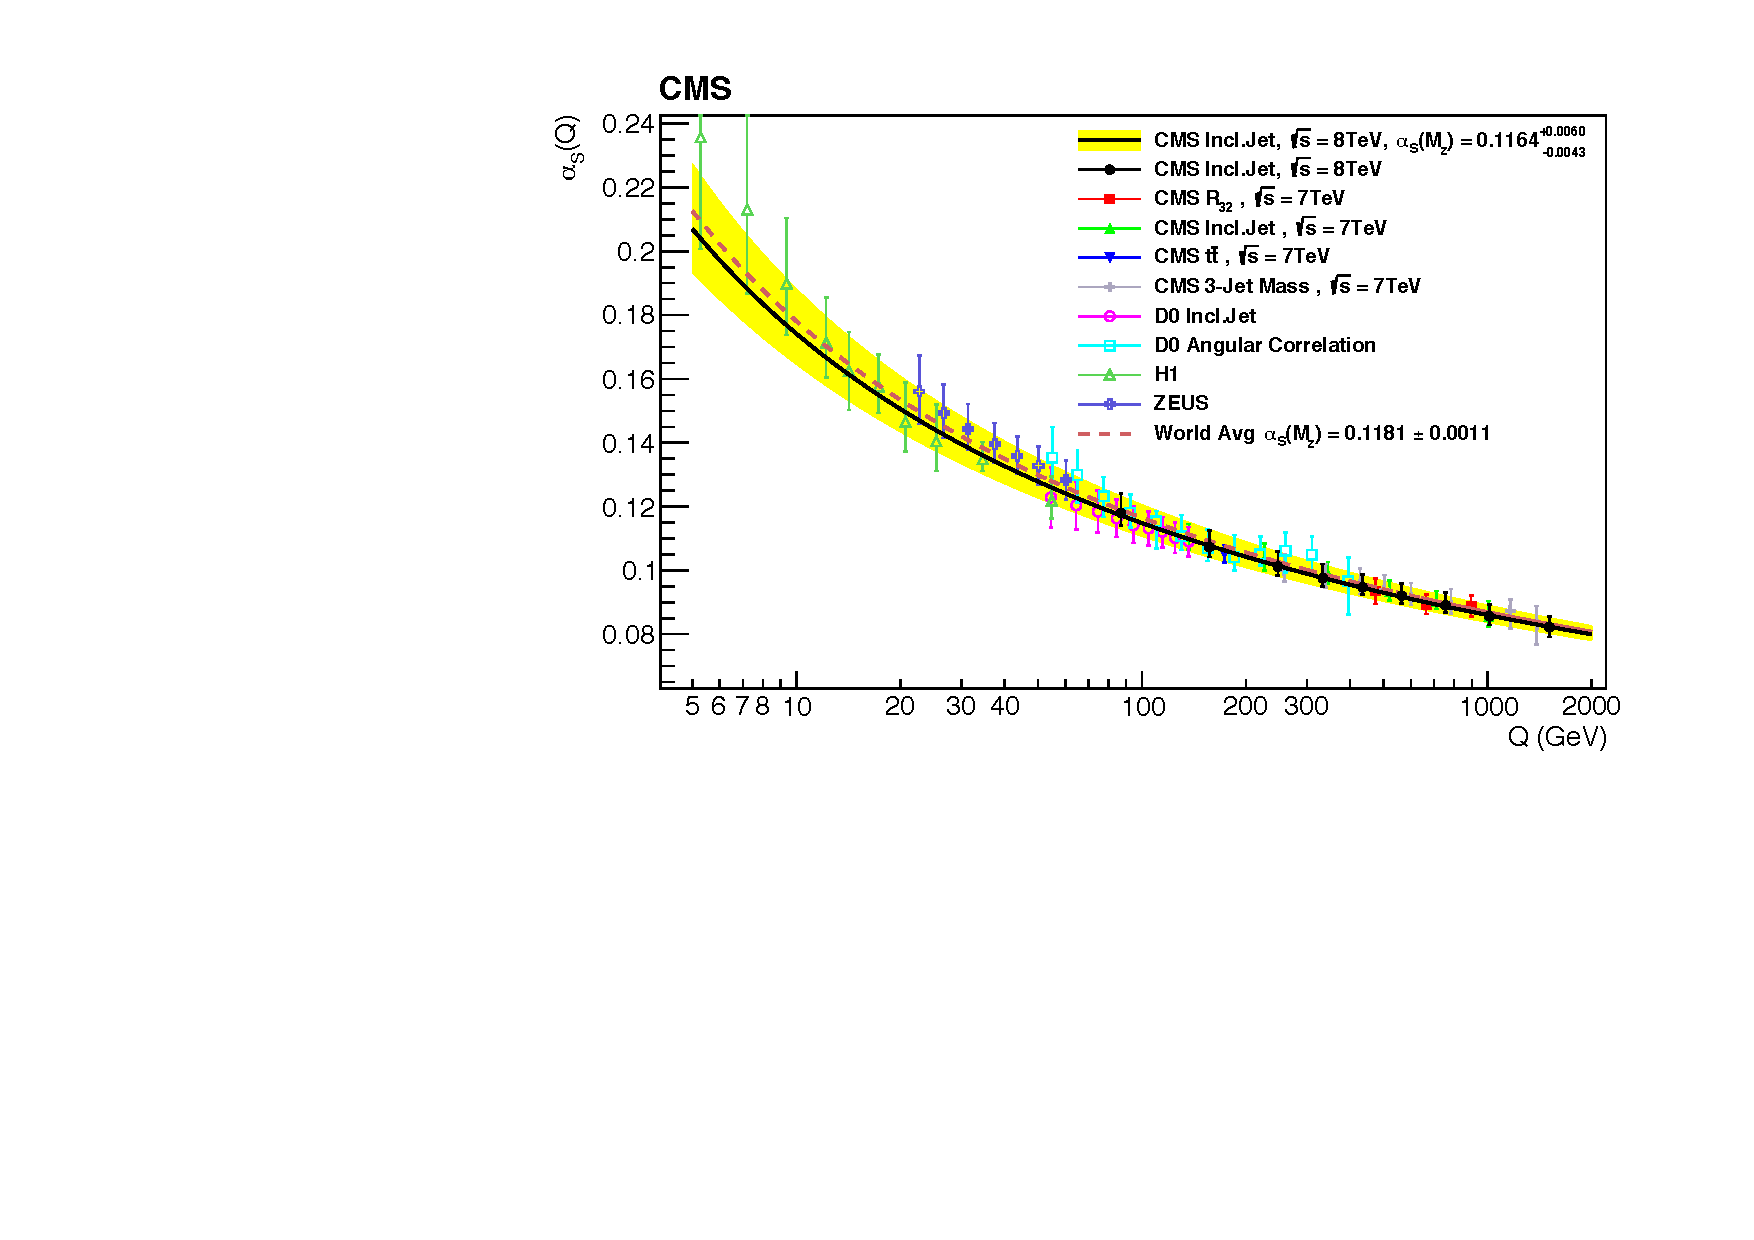
\includegraphics[width=0.7\textwidth]{Figures/standard_model/running}
    \caption{The running of the strong coupling constant $\alpha_s = \sfrac{g_s^2}{4\pi}$ as a function of the energy scale $Q$ as measured by experiments at the LHC, Tevatron, and HERA~\cite{CMSRunning}.}
    \label{fig:asymptotic_freedom}
\end{figure}

An observed effect of QCD is \textit{colour confinement} where quarks and gluons are never observed in isolation, but are always bound together in colour-neutral ($\text{SU}(3)$ invariant) states called hadrons.
This is illustrated by the qualitative picture in \Cref{fig:confinement}.
For an electromagnetic interaction, \Cref{fig:confinement_b}, the field is diluted over space.
However, for a strong interaction, \Cref{fig:confinement_c}, the exchanged gluons themselves interact, \Cref{fig:confinement_a}, effectively squeezing the colour field between the quarks into a \textit{colour flux tube} or a \textit{colour string}.
These strings have a constant energy density so two free quarks on opposite sides of the universe would theoretically result in a string of near-infinite energy.
As the theory is non-perturbative, there is no analytical description for confinement.
A consequence of confinement is hadronisation, the process by which high energy coloured particles form particle jets, which is described in \Cref{sec:jets}.

\begin{figure}[h]
    \centering
    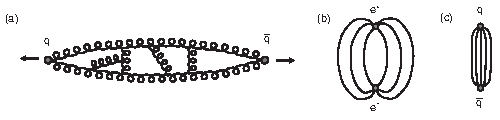
\includegraphics[width=0.8\textwidth]{Figures/standard_model/confinement.pdf}
    \begin{subfigure}{0pt}\phantomcaption{}\label{fig:confinement_a}\end{subfigure}
    \begin{subfigure}{0pt}\phantomcaption{}\label{fig:confinement_b}\end{subfigure}
    \begin{subfigure}{0pt}\phantomcaption{}\label{fig:confinement_c}\end{subfigure}
    \caption{Qualitative picture of the formation of colour strings due to interaction between the exchanged gluons from two quarks \cite{ModernParticlePhysics}.}.
    \label{fig:confinement}
\end{figure}

\subsection{\texorpdfstring{$\text{SU}(2)_L \times \text{U}(1)_Y \rightarrow$}{SU(2)xSU(1)-} Electroweak Theory}
\label{sec:electroweak}

In 1934 Fermi's description of $\beta$ decay~\cite{Fermi1934} hypothesized the existence of the weak nuclear force and allowed for the creation and annihilation of particles.
Around three decades later the Glashow-Weinberg-Salam model (GSW)~\cite{Glashow1961, Weinberg1967,Salam1964} was developed to unify the electromagnetic and weak forces using the combined $\text{SU}(2)_L \times \text{U}(1)_Y$.
As with all gauge theories, this introduces four gauge fields corresponding to each generator of the group.
\begin{align}
    \text{SU}(2)_L & \rightarrow W_\mu^a(a = 1, 2, 3) \\
    \text{U}(1)_Y  & \rightarrow B_\mu
\end{align}
The $\text{SU}(2)_L$ group is non-Abelian making this a Yang-Mills theory, and the structure constants are given by $f^{abc} = \epsilon^{abc}$, where $\epsilon^{abc}$ is the Levi-Civita symbol.
The generators of the group are the based on the three Pauli spin matrices $\sigma^i$.
\begin{equation}
    \label{eq:su2_generators}
    T^a \equiv I^a = \frac{\sigma^a}{2} \\
\end{equation}
\begin{equation}
    \sigma^1 = \begin{pmatrix} 0 & 1 \\ 1 & 0 \end{pmatrix},
    \quad \sigma^2 = \begin{pmatrix} 0 & -i \\ i & 0 \end{pmatrix},
    \quad \sigma^3 = \begin{pmatrix} 1 & 0 \\ 0 & -1 \end{pmatrix}.
    \label{eq:pauli_matrices}
\end{equation}
The strength tensors are given by
\begin{align}
    \label{eq:ew_field_strength_tensors}
    W_{\mu\nu}^a & = \partial_\mu W_\nu^a - \partial_\nu W_\mu^a - g \epsilon^{abc} W_\mu^b W_\nu^c, \\
    B_{\mu\nu}   & = \partial_\mu B_\nu - \partial_\nu B_\mu.
\end{align}
It is useful to split the fermion fields into left- and right-handed components using the chiral projection operators $P_{L/R} = \sfrac{1}{2} (1 \mp \gamma^5)$, where $\gamma^5 = i \gamma^0 \gamma^1 \gamma^2 \gamma^3$.
Experimentally the charged weak current has proved to maximally violate $\mathcal{P}$ symmetry.
This means that the interaction term must follow a V-A (vector-axial) coupling type which can be shown to be equivalent to a standard coupling to left-handed fermions only:
\begin{equation}
    \label{eq:v-a_coupling}
    \mathcal{L}_\text{V-A}
    = \frac{1}{2} \bar \psi \gamma^\mu (1 - \gamma^5) \psi W_\mu
    = \bar \psi \gamma^\mu P_L \psi W_\mu
    = \bar \psi P_R \gamma^\mu P_L \psi W_\mu
    = \bar \psi_L \gamma^\mu \psi_L W_\mu.
\end{equation}
Therefore, only left-handed fermions (and right-handed antifermions) carry non-zero weak isospin.
The covariant derivative is given by,
\begin{equation}
    \label{eq:ew_covariant_derivative}
    D_\mu = \partial_\mu - i g_W \frac{\sigma_a}{2} W_\mu^a - i g_Y \frac{Y}{2} B_\mu,
\end{equation}
where $g_W$ and $g_Y$ are the weak and hypercharge coupling constants respectively.
The Lagrangian for electroweak theory is,
\begin{align}
    \begin{split}
        \label{eq:ew_lagrangian}
        \mathcal{L}_\text{EW} = & - \bar{\psi}_L \left( \gamma^\mu g_W \frac{1}{2} \sigma^a W^a_\mu + \gamma^\mu g_Y \frac{Y}{2} B_\mu \right) \psi_L - \bar{\psi}_R \left( \gamma^\mu g_Y \frac{Y}{2} B_\mu \right) \psi_R \\
                                & - \frac{1}{4} W_{\mu\nu}^a W^{a,\mu\nu} - \frac{1}{4} B_{\mu\nu} B^{\mu\nu}.
    \end{split}
\end{align}
As a Yang-Mills theory, the gauge fields $W_\mu^a$ interact in quadratic and triple self-couplings.

The $2 \times 2$ Pauli matrices require two new components to the fermion wave function which are described as weak isospin doubles.
The left-handed fermions (and right-handed antifermions)
are placed in doublets which differ by a unit of charge.
Up-type quarks and neutrinos have a weak isospin of $\sfrac{1}{2}$, while down-type quarks and charged leptons have a weak isospin of $-\sfrac{1}{2}$.
The corresponding weak eigenstate doublets are given by,
\begin{equation}
    \label{eq:weak_isospin}
    \begin{pmatrix} \nu_e \\ e \end{pmatrix}_L,
    \begin{pmatrix} \nu_\mu \\ \mu \end{pmatrix}_L,
    \begin{pmatrix} \nu_\tau \\ \tau \end{pmatrix}_L,
    \begin{pmatrix} u \\ d' \end{pmatrix}_L,
    \begin{pmatrix} c \\ s' \end{pmatrix}_L,
    \begin{pmatrix} t \\ b' \end{pmatrix}_L.
\end{equation}
The right-handed fermions (and left-handed antifermions) do not carry isospin and are placed in singlets.
The effect of the charged weak interaction is therefore to rotate these doublets, effectively changing the flavour of the fermion\footnote{Since there is no other force through which the neutrinos can interact, there are no right-handed neutrinos in the SM.}.

The isospin doublets are described with respect to the weak eigenstates, which do not correspond to the observable mass eigenstates.
The down-type quarks by convention mix between the weak eigenstates ($d', s', b'$) and the mass eigenstates ($d, s, b$) through the CKM matrix~\cite{cabibbo1963},
\begin{equation}
    \label{eq:ckm_matrix}
    \begin{pmatrix} d' \\ s' \\ b' \end{pmatrix} =
    \begin{pmatrix} V_{ud} & V_{us} & V_{ub} \\ V_{cd} & V_{cs} & V_{cb} \\ V_{td} & V_{ts} & V_{tb} \end{pmatrix} \begin{pmatrix} d \\ s \\ b \end{pmatrix} =
    \begin{pmatrix} 0.974 & 0.224 & 0.004 \\ 0.221 & 0.975 & 0.041 \\ 0.009 & 0.042 & 1.014 \end{pmatrix} \begin{pmatrix} d \\ s \\ b \end{pmatrix},
\end{equation}
where the numerical values of the elements are determined experimentally~\cite{ParticleDataGroup}\footnote{The non-unitary nature of experimental values of the CKM matrix is in tension with the SM by 2.2$\sigma$}.
For the leptons, mixing is described with respect to the neutrinos and the PMNS matrix~\cite{PMNSMatrix}.
These matrices provide explanations for the observed neutrino oscillations and the CP violation of the weak sector.

\section{Electroweak Symmetry Breaking}
\label{sec:higgs}

GSW theory predicts 4 gauge fields $W^a_\mu$ and $B_\mu$ which do not correspond to the physical $W^\pm$, $Z$, and $\gamma$ bosons.
As a requirement of gauge invariance these fields are deemed to be massless, which is in contradiction to the observed massive $W^\pm$ and $Z$ bosons.
These discrepancies are resolved by the Brout-Englert-Higgs mechanism~\cite{Higgs1, Higgs2, Higgs3} (referred to hereafter as the Higgs mechanism), and the spontaneous symmetry breaking of the electroweak symmetry group (EWSB).
Spontaneous symmetry breaking is a phenomenon where the ground state of a system does not exhibit the same symmetries of the Lagrangian.
Experimental evidence for the electroweak theory first came in 1983 with the discovery of the W and Z bosons at CERN\@~\cite{WZ}.
Arguably the last major breakthrough in the field of particle physics was the discovery of the Higgs boson in 2012 by the ATLAS and CMS collaborations~\cite{ATLASHiggs, CMSHiggs}.

Consider a new scalar field given by a complex doublet,
\begin{equation}
    \phi = \begin{pmatrix} \phi^+ \\ \phi^0 \end{pmatrix} = \frac{1}{\sqrt{2}} \begin{pmatrix} \phi_1 + i \phi_2 \\ \phi_3 + i \phi_4 \end{pmatrix},
\end{equation}
embedded in a theory which observes the local $\text{SU}(2)_L \times \text{U}(1)_Y$ symmetry of the GSW model.
The Lagrangian density for the free scalar field, defined with the same covariant derivatives of \Cref{eq:ew_covariant_derivative}, is given by,
\begin{equation}
    \label{eq:higgs_lagrangian}
    \mathcal{L} = (D_\mu \phi)^\dagger (D^\mu \phi) - V(\phi).
\end{equation}
Here, $V(\phi)$ is a potential term describing the field self-interactions.
The specific potential encountered in the Higgs mechanism is defined as,
\begin{equation}
    \label{eq:higgs_potential}
    V(\phi) = \mu^2 \phi^\dagger \phi + \lambda (\phi^\dagger \phi)^2,
\end{equation}
where $\mu^2$ and $\lambda$ are free parameters of the theory with some restrictions.
The value of $\lambda$ is required to be positive to ensure the potential is bounded from below, allowing a stable vacuum state (the state of lowest energy).
The value of $\mu^2$ is constrained to be negative to allow for spontaneous symmetry breaking.
The vacuum state is found by minimizing the Hamiltonian of a system which corresponds to,
\begin{equation}
    \frac{\partial V}{\partial \phi} = 0 \Longrightarrow  \phi^\dagger \phi = -\frac{\mu^2}{2\lambda} \equiv \frac{v^2}{2},
\end{equation}
where $v$ is the vacuum expectation value of the field.

\begin{figure}[h]
    \centering
    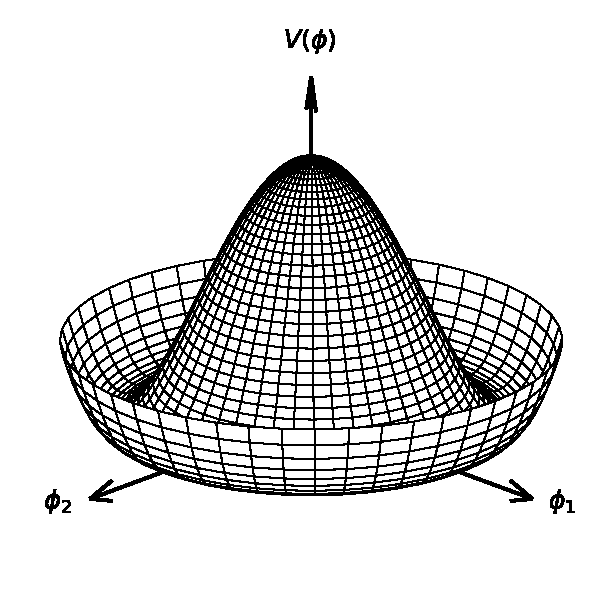
\includegraphics[width=0.5\textwidth]{Figures/standard_model/mexican_hat_potential}
    \caption{The form of the Higgs potential $V(\phi)$ if $\mu^2 < 0$ and $\lambda > 0$ respect to the first component of the complex doublet}
    \label{fig:mexican_hat}
\end{figure}

As shown in \Cref{fig:mexican_hat}, the potential has an infinite number of vacuum states satisfying this condition.
Physically the vacuum will fall into one of these states, spontaneously breaking the symmetry of the Lagrangian.
With no loss of generality, the physical vacuum state is chosen to be,
\begin{equation}
    \label{eq:higgs_vacuum}
    | 0 \rangle	= \frac{1}{\sqrt{2}} \begin{pmatrix} 0 \\ v \end{pmatrix}.
\end{equation}
In order to use perturbation theory the field $\phi$ is expanded about the vacuum state $|0\rangle$,
\begin{equation}
    \phi(x) = \frac{1}{\sqrt{2}} \begin{pmatrix} \phi_1(x) + i \phi_2(x) \\ v + \phi_3 + i \phi_4(x) \end{pmatrix}.
\end{equation}

The expected form of the symmetry breaking should result in the group of QED,
\begin{equation}
    \text{SU}(2)_L \times \text{U}(1)_Y \rightarrow_\text{EWSB} \text{U}(1)_\text{Q},
\end{equation}
where $Q$ refers to the electric charge.
The Goldstone theorem states that for every spontaneously broken continuous symmetry there exists a massless scalar boson; one for each generator of the group.
In EWSB, the broken symmetry should result in three massless Goldstone bosons, however there is no experimental evidence for such massless scalar particles.
The Higgs mechanism resolves this by absorbing the Goldstone bosons through an appropriate selection of gauge.
It's crucial to note that physical predictions remain unchanged regardless of the gauge, but by selecting the \textit{unitary gauge}, the Goldstone bosons vanish, and the fields in the Lagrangian represent the actual physical particles.
In the unitary gauge the scalar field is given by,
\begin{equation}
    \label{eq:higgs_unitary_gauge}
    \phi(x) = \frac{1}{\sqrt{2}} \begin{pmatrix} 0 \\ v + h(x) \end{pmatrix},
\end{equation}
where $h(x)$ is the physical massive Higgs field, the excitation of which is the Higgs boson $H$.

The relationship between weak isospin, hypercharge, and electric charge is given by,
\begin{equation}
    \label{eq:hypercharge}
    Q = I^3 + \frac{Y}{2}.
\end{equation}
Because the only surviving massless boson is the photon, $\text{U}(1)_\text{Q}$ must remain a symmetry of the vacuum state.
This is achieved by setting the electric charge of the vacuum state to zero, or equivalently $Y=1$.
Using the definitions from \Cref{eq:pauli_matrices} and \Cref{eq:ew_covariant_derivative} the covariant derivative is given by,
\begin{equation}
    \label{eq:higgs_covariant_derivative}
    D_\mu = \frac{1}{2}
    \begin{pmatrix}
        2 \partial_\mu + i g_W W_\mu^3 + i g_Y B_\mu &
        i g_W (W_\mu^1 - i W_\mu^2)                    \\
        i g_W (W_\mu^1 + i W_\mu^2)                  &
        2 \partial_\mu - i g_W W_\mu^3 + i g_Y B_\mu.
    \end{pmatrix}
\end{equation}
Combining this with the unitary gauge scalar field yields the first term of the Higgs Lagrangian,
\begin{align}
    \label{eq:higgs_lagrangian_1}
    \begin{split}
        (D_\mu \phi)^\dagger (D^\mu \phi) =
        \frac{1}{2} \partial_\mu h \partial^\mu h
        + \frac{1}{8} g_W^2 (W_\mu^1 + i W_\mu^2)(W^{1\mu} - i W^{2\mu})(v + h)^2
        \\
        + \frac{1}{8} (g_W W_\mu^3 - g_Y B_\mu)(g_W W^{3\mu} - g_Y B^\mu)(v + h)^2.
    \end{split}
\end{align}
One can identify the massive physical fields by the terms in \Cref{eq:higgs_lagrangian_1} that are quadratic in the gauge boson fields and do not contain the Higgs field.
\begin{equation}
    W^\pm_\mu = \frac{W^1_\mu \mp i W^2_\mu}{\sqrt{2}}
    \qquad
    Z_\mu = \frac{g_W W^3_\mu - g_Y B_\mu}{\sqrt{g_W^2 + g_Y^2}}
    \qquad
    A_\mu = \frac{g_W B_\mu + g_Y W^3_\mu}{\sqrt{g_W^2 + g_Y^2}}.
\end{equation}
Rewriting out \Cref{eq:higgs_lagrangian} in terms of the physical fields and in the unitary gauge gives,
\begin{equation}
    \label{eq:higgs_lagrangian_full}
    \resizebox{.99\hsize}{!}{$
            \begin{aligned}
                \mathcal{L}_{EW+H}
                 & = \underbrace{\vphantom{\frac{}{}} - \lambda v^2 h^2}_{H \text{ mass}}
                \underbrace{+\frac{1}{4} g_W^2 v^2 W^-_\mu W^{+\mu}}_{W \text{ mass}}
                \underbrace{+\frac{1}{8} g_Y^2 v^2 Z_\mu Z^\mu}_{Z \text{ mass}}                                                                                 \\
                 & \underbrace{+\frac{1}{2} g_W^2 v h W^-_\mu W^{+\mu}}_{HWW}
                \underbrace{+\frac{1}{4} g_W^2 h^2 W^-_\mu W^{+\mu}}_{HHWW}
                \underbrace{+\frac{1}{4} g_Y^2 v h Z_\mu Z^\mu}_{HZZ}
                \underbrace{+\frac{1}{8} g_Y^2 h^2 Z_\mu Z^\mu}_{HHZZ}                                                                                           \\
                 & \underbrace{+\frac{1}{2}(\partial_{\mu} h)(\partial^{\mu} h) - \lambda v h^3 + \frac{1}{4}\lambda h^4}_{h\text{ dynamics and self-couplings}}
                \underbrace{+\frac{1}{4} W^a_{\mu\nu} W^{a,\mu\nu} + \frac{1}{4} B_{\mu\nu} B^{\mu\nu}}_{\text{EW dynamics and self-couplings}}.
            \end{aligned}
        $}
\end{equation}
From the top row of \Cref{eq:higgs_lagrangian_full} the masses of each of the bosons can be identified,
\begin{equation}
    \label{eq:ew_masses}
    m_W = \frac{1}{2} g_W v
    \qquad
    m_Z = \frac{1}{2} v \sqrt{g_W^2 + g_Y^2}
    \qquad
    m_A = 0
    \quad
    m_H = \sqrt{2 \lambda} v.
\end{equation}
For convenience, the bottom row of \Cref{eq:higgs_lagrangian_full} includes the dynamics and self-couplings of the electroweak fields in their original form before EWSB.
Expanding this term with respect to the physical fields results in trilinear interactions between the photon and the $W^\pm$ bosons.
The free parameters of the GSW + Higgs mechanism are the electroweak coupling constants $g_W$ and $g_Y$, the Higgs self-coupling $\lambda$, and the vacuum expectation value $v$, all of which are determined experimentally.

The final piece of the SM is the generation of fermion masses through the Higgs mechanism.
Due to the different transformation properties of the left- and right-handed fermions, the standard mass term $m \bar \psi \psi$ mixes the left- and right-handed components and thus is not invariant under the electroweak symmetry group.
The Yukawa interaction term is introduced to couple each of the fermions doublets to the Higgs field.
For example the electron mass term is given by,
\begin{equation}
    \label{eq:yukawa}
    \begin{split}
        \mathcal{L}_\text{Yukawa} & = -g_e( \bar \psi_L \phi \psi_R + \bar \psi_R \phi^\dagger \psi_L)    \\
                                  & = -g_e \left[
            \begin{pmatrix} \bar \nu_e & \bar e \end{pmatrix}_L \begin{pmatrix} 0 \\ \frac{v + h}{\sqrt{2}} \end{pmatrix} e_R
            + \bar e_R \begin{pmatrix} 0 & \frac{v + h}{\sqrt{2}} \end{pmatrix} \begin{pmatrix} \nu_e \\ e \end{pmatrix}_L
        \right]                                                                                           \\
                                  & = -\frac{g_e v}{\sqrt{2}} \bar e e - \frac{g_e}{\sqrt{2}} \bar e e h,
    \end{split}
\end{equation}
where $g_e$ is the electron Yukawa coupling constant.
A similar prescription can be applied to other leptons, the up-type, and down-type quarks to yield the relationship of the fermion masses $m_f$ to the Yukawa coupling constants $g_f$ and the Higgs vacuum expectation value,
\begin{equation}
    \label{eq:fermion_mass}
    m_f = \frac{g_f v}{\sqrt{2}}.
\end{equation}

\section{Particle Jets}
\label{sec:jets}

In particle physics, jets are collimated streams of particles moving together in a cone-like structure that were initiated by a high-energy quark or gluon.
A common feature in high-energy collisions, jets are emergent phenomena that arise due to the nature of QCD.
Simply put, if a high-energy quark or gluon is emitted from a collision, it quickly radiates gluons.
Each of these emissions can themselves radiate gluons or split into quark-antiquark pairs, starting the process anew.
This continues until the energy of the particles is low enough that they form stable colour-neutral bound states.
Jets are therefore formed during the transition from the perturbative to the non-perturbative regimes of QCD.

Jet formation can be highlighted by the Feynman diagram in \Cref{fig:quark_gluon}.
Here a quark propagator, produced in some inelastic collision, radiates a gluon.
This matrix element becomes dominant when the virtual propagator is close to being on-shell.
This condition is satisfied by two limits which are essential in jet physics.
One is referred to as the \textit{collinear limit} where the angle between the quark and the gluon approaches zero.
This indicates preference for collinear radiation and explains why jets are collimated in the direction of the initiating particle\footnote{Jets are also collimated when measured in the lab frame due to the large boost of the initiating particle.}.
The other is the \textit{soft limit} where the energy of the gluon approaches zero.
Practically, this means that each time a parton is emitted, it is accompanied by a soft haze of radiation.
These conditions exist for all gauge theories, but are particularly important for QCD due the strength of $\alpha_s$ even at high energies.

\begin{figure}[h]
    \centering
    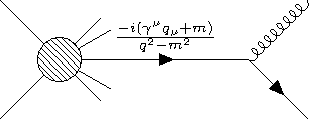
\includegraphics[width=0.5\textwidth]{Feynman/quark_gluon.pdf}
    \caption{Simple diagram of a quark emitted from a collision radiating a gluon. The matrix element of this process has a singularity when the virtual propagator is close to being on-shell ($q^2\approx m^2$) which is satisfied in the collinear and soft limits.}
    \label{fig:quark_gluon}
\end{figure}

Another view of jet formation is through the process of breaking colour strings between quarks.
From confinement, if two quarks were produced back-to-back in a collision, the colour field between them would be squeezed into a colour string with constant energy density.
As they move apart it becomes energetically favourable to create a quark-antiquark pair from the vacuum, leading to two new strings.
If the quarks are produced with enough energy, this process repeats until the energy is low enough that the stable colour-neutral bound states emerge as shown by \Cref{fig:hadronisation}.
Where exactly the strings break is ambiguous, resulting in the highly stochastic nature of jets.
The lightest hadrons are the most accessible to this process, which is why typically jets are composed primarily of pions ($\approx80\%$) and kaons ($\approx15\%$).

\begin{figure}[h]
    \centering
    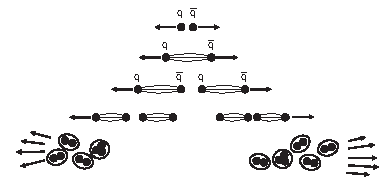
\includegraphics[width=0.8\textwidth]{Figures/standard_model/hadronisation.pdf}
    \caption{Qualitative picture of the formation of two jets via the splitting of colour flux-tubes causing hadronisation \cite{ModernParticlePhysics}.}
    \label{fig:hadronisation}
\end{figure}

While jets are essentially sets or clusters of many particles, they can also be defined by their own kinematics, calculated by summing up the four-momenta of all of their constituents.
Furthermore, even if the original parton was massless, the jet as a whole may have non-zero invariant mass due to noncollinear radiation.
The nature and shape of this radiation is characteristic of the properties of the initiating parton.
This point is crucial for understanding jet physics and defining jet reconstruction algorithms.

\section{Standard Model Limitations and Open Questions}
\label{sec:sm_limitations}

Predictions made by the SM have been confirmed to an extraordinary degree of precision in collider experiments, as shown by \Cref{fig:sm_precision}.
Despite this, there are several reasons to believe that the SM is not the final theory of particle physics.
Many perceived shortcomings of the SM lead to open questions, active areas of research, and proposed extensions to the theory.

For example, gravity is a notable omission from the SM owing to the lack of a renormalizable QFT for gravity.
Candidate theories for a quantum theory of gravity include string theory and loop quantum gravity~\cite{GravityQFT}.
However, gravity is so weak that it is unlikely a theory of quantized gravity could even make testable predictions at the energies accessible by current experiments.

\begin{figure}
    \centering
    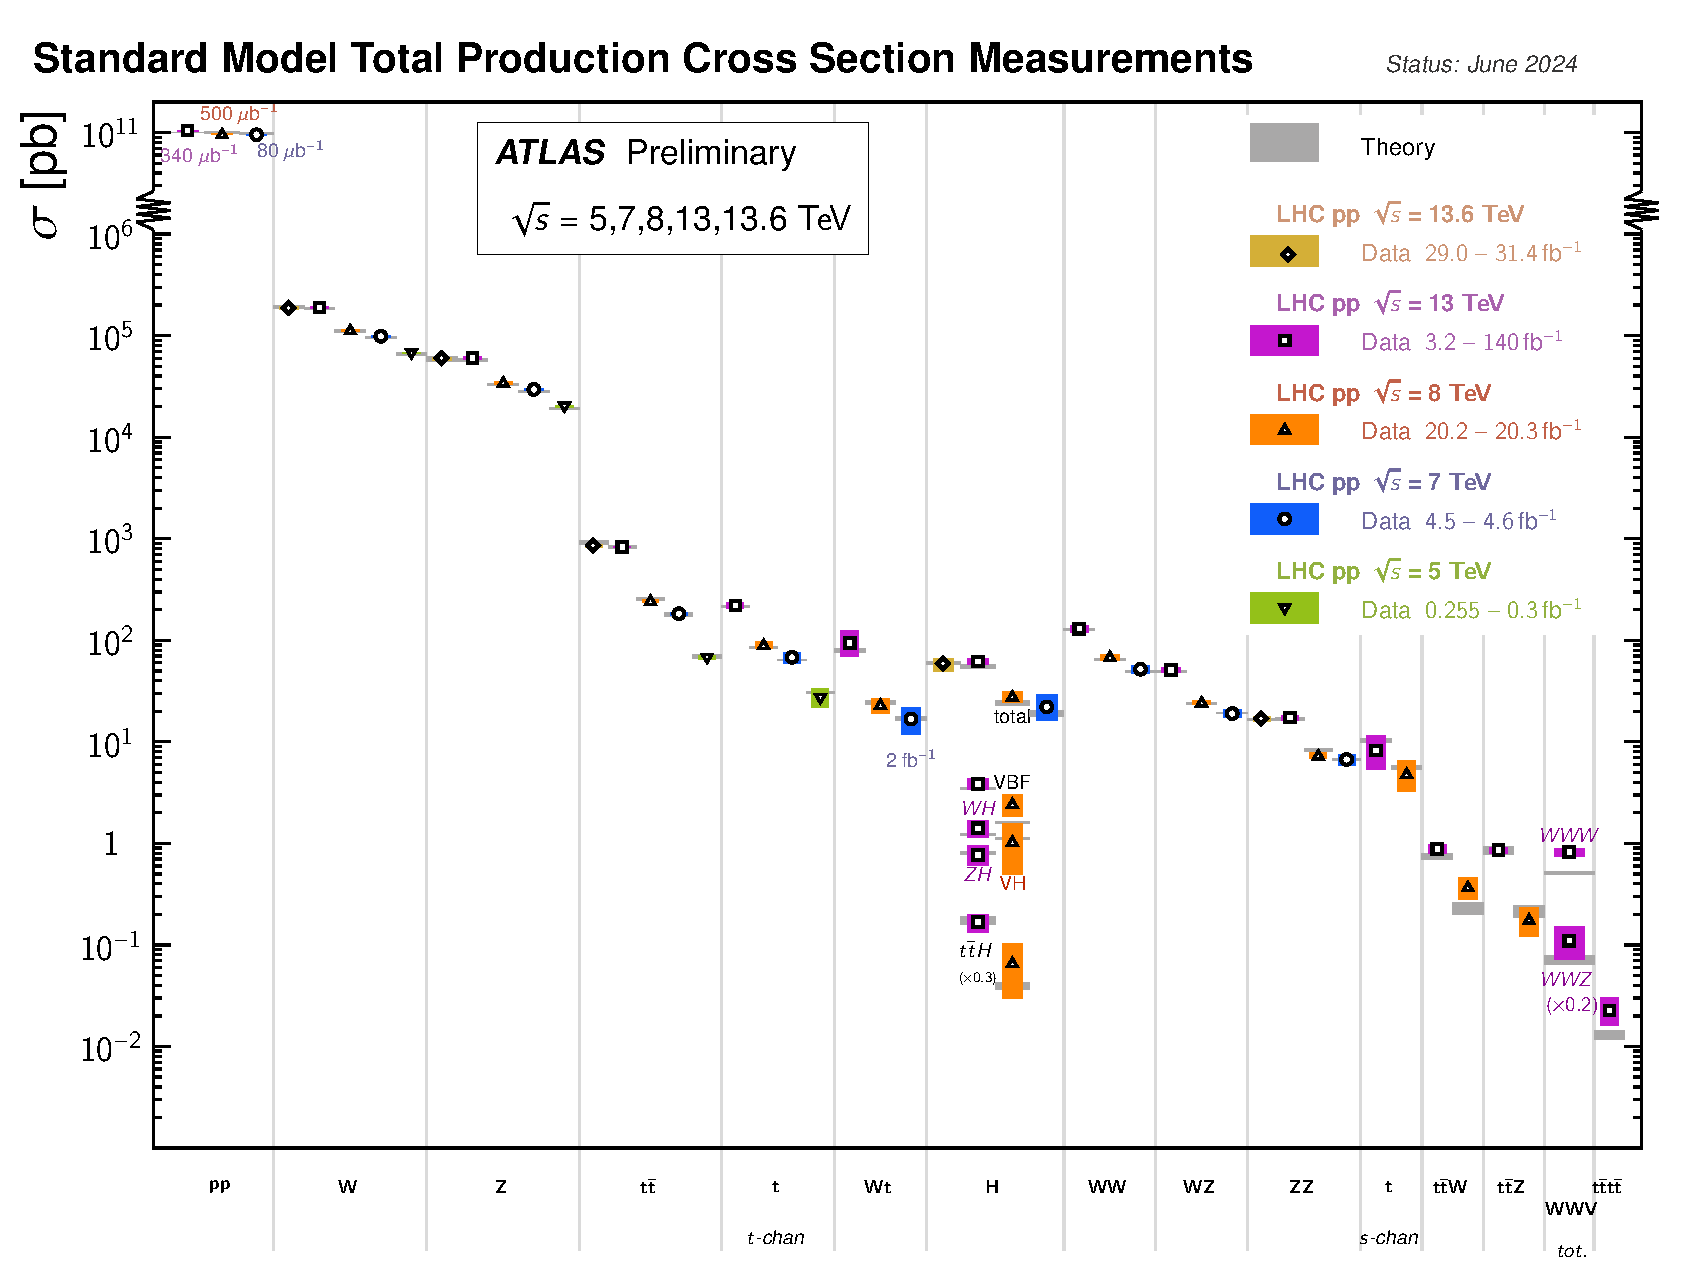
\includegraphics[width=0.7\textwidth]{Figures/standard_model/sm_summary.pdf}
    \caption{Comparison of the total production cross-sections of various processes predicted by the SM and measured by the ATLAS experiment \cite{ATLAS:2024cgh}.}
    \label{fig:sm_precision}
\end{figure}

Cosmological observations dating back to the 1930s~\cite{GalaxyRotation} have shown that the majority of the gravitational effects in the universe is not a result of visible matter.
This was first observed by the movements of galaxies within clusters~\cite{GalaxyRotation}, but has since been independently supported by measurements of the rotation of galaxies themselves~\cite{DistributionDarkMatter, EvidenceDarkMatter,NumericalStudyStability}, gravitational lensing~\cite{GravitationalLensMagnification, Lensing1, Lensing2},
hot gas in galaxy clusters~\cite{HotGas}, and the cosmic microwave background~\cite{Planck2018Results}.
The current theory to explain these phenomena is the presence of cold dark matter (CDM) which accounts for 85\% of the mass content in the universe~\cite{Planck2018Results}.
In this model, CDM particles must be stable, massive, and (at most) weakly interacting.
There is no candidate in the SM that fits this description.
Furthermore, in the $\Lambda$CDM model of cosmology the dominant energy in the universe is \textit{dark energy}~\cite{LCDM1, LCDM2, LCDM3, LCDM4}, a positive pressure of the vacuum causing the universe to expand at an accelerating rate for which the SM offers no explanation.

In the SM, anti-matter is treated as a mirror image of matter.
However, there is a significant discrepancy between the amount of matter and anti-matter in the universe~\cite{AlexDM1, AlexDM2}.
There exist two possibilities for this discrepancy; either the universe began with a preference for matter over anti-matter, or the universe was initially symmetric, and some process called \textit{baryogenesis}~\cite{BaryosynthesisOriginGalaxies}, occurred to create the imbalance.
While there is no clear evidence for either scenario, the latter is more appealing to many physicists.
The Sakharov conditions~\cite{Sakharov1967} for baryogenesis are that it violates baryon number, C and CP symmetry, and must have occurred before the universe reached thermal equilibrium.
CP violation is present in the SM from the CKM and PMNS matrices, but it is not sufficient to explain the observed matter-antimatter asymmetry.
It is hoped that there exists new physical processes beyond the SM that induces the much larger CP violation required for baryogenesis.

The above issues are associated with the SM's inability to describe cosmological phenomena.
An additional set of ``issues'' are derived from aesthetic or philosophical considerations.
The SM has 19 free parameters that must be determined experimentally, a value considered by many to be too large to be considered a fundamental theory.
Another issue is the \textit{hierarchy problem}.
In a QFT, physical observables are determined by the sum of all possible Feynman diagrams, which often includes divergent terms.
These divergences are removed by renormalization which fixes the parameters of the theory to the observed values.
However, in the case of the Higgs mass, the one-loop corrections are around 16 orders of magnitude larger than the observed value.
To resolve this the bare mass of the Higgs must be fine-tuned to an accuracy of 1 part in $10^{16}$, which many physicists find unsatisfactory.
Finally, the unification of QED and the weak force led many physicists to develop Grand Unified Theories (GUTs)~\cite{GUT1, GUT2} which predict that all forces in the SM are unified at high energies.
Many of the predictions of GUTs, such as proton decay, have not been observed, and the energy scale at which the forces unify is far beyond the reach of current experiments.

% 
\chapter{The Large Hadron Collider and the ATLAS Detector}
\label{ch:lhc_atlas_detector}

The Large Hadron Collider (LHC)~\cite{LHCMachine,LHC1,LHC2, LHC3} is a synchrotron collider located at the Conseil Européen pour la Recherche Nucléaire (CERN) near Geneva, Switzerland.
It is also the world's most powerful particle accelerator, providing both proton-proton ($pp$) and heavy ion collisions at the high energy frontier.
At maximum speed, the protons in the LHC are only $3~\mps$ slower than the speed of light.

Four primary experiments utilize the $\TeV$ scale collisions generated at each of the four interaction points (IPs) of the LHC.
Two general-purpose experiments, ATLAS~\cite{ATLAS} and CMS~\cite{CMS}, employ hermetic detectors to study various physics processes.
The LHCb experiment~\cite{LHCb} focuses on measuring the properties of B mesons and other particles containing b-quarks, which are significant for understanding CP violation.
The Alice experiment~\cite{ALICE} investigates the properties of quark-gluon plasma, a state of matter believed to have existed in the early universe.
Additionally, the LHC hosts several smaller, highly specialized experiments including LHCf~\cite{LHCf}, TOTEM~\cite{TOTEM}, MoEDAL~\cite{MoEDAL}, FASER~\cite{FASER}, and SND@LHC~\cite{SNDLHC}.
All LHC experiments strive to answer fundamental questions about the universe; to test the predictions of the Standard Model of particle physics or to search for new physics beyond it.

This section describes common collider physics definitions, such as the coordinate system and luminosity,
the LHC along with its injector chain, and the ATLAS experiment.
As the focus of this work is on data and tools for $pp$ collisions at the LHC, the discussion is limited to this context.
Additionally, the components of this thesis which utilized official ATLAS simulation and software, \Cref{ch:spice}, were limited to tracks and jets.
Therefore, the information provided here is focused on these topics only.

\section{The Large Hadron Collider}

The LHC is a somewhat circular collider with a circumference of $26.7~\km$.
It is closer to an irregular octagon with rounded corners and approximately $ 530~\m $ long straight sections, housed within a tunnel whose depth varies between $45~\m$ and $170~\m$ underground.

The machine consists of two ring acceleration pipes, each carrying a separate beam of protons or heavy ions that are accelerated in opposite directions.
The beams are surrounded by 1232 superconducting niobium-titanium (NbTi) dipole magnets that generate an $8.33~\tesla$ magnetic field to bend the protons around the curved sections of the ring.
Many more higher-order multipole magnets are used for beam insertion, cleaning, dumping, and focusing towards the experiment IPs.
Along one of the straight sections, 16 superconducting radiofrequency cavities, eight per beam, operate at $400~\MHz$ to accelerate the protons to their maximum energy.
The LHC was designed to deliver a centre-of-mass energy of $\sqrt{s}=14~\TeV$ but has yet to reach this due to technical limitations.

The beams are not continuous streams of protons but are instead segmented into bunches, each containing on the order of $10^{11}$ particles.
The radiofrequency cavities are tuned to ensure that these bunches are tightly packed, each as long as $7.5~\cm$ and separated by only $25~\ns$.
For collisions to occur, the bunches from the two opposing beams are compressed to a space of $64~\um$, around the width of a strand of hair, and made to pass through each other.
Even with such compression and more than a hundred billion protons in each bunch, the average number of interactions per bunch crossing \avemu is less than 100.

\subsection{The CERN Accelerator Complex}

The LHC is a synchrotron, meaning that it cannot accelerate particles from rest.
Therefore, it is only the final stage of the CERN accelerator complex, which is shown in \Cref{fig:cern_accelerator_complex}.
Each stage in the chain of accelerators increases the energy of the particles within before passing them to the next stage.
Before 2020, the chain began with the Linear Accelerator (Linac) 2, which accelerated protons to $50~\MeV$.
The input to Linac2 was hydrogen gas, stripped of its electrons by a strong electric field.
Following Run 2, the chain was updated to begin with Linac4, which operates on negative hydrogen ions, not protons.
This change reduces the beam loss, allowing more particles to accumulate in the next stage.
Furthermore, Linac4 introduce a three-fold increase in beam energy, outputting particles at $160~\MeV$.
The Linacs feed the Proton Synchrotron Booster (PSB), which increases the energy to $2~\GeV$ and also serves to strip the electrons from the hydrogen ions.
From the PSB, the protons are passed to the Proton Synchrotron (PS), which accelerates them to $26~\GeV$, and then to the Super Proton Synchrotron (SPS), which accelerates them to $450~\GeV$.
From there, they are injected into the LHC.
This entire process takes a few seconds, but several minutes are required to fill the entire bunch train of the LHC.
The LHC then accelerates the bunches to the final energy, which, as of Run 3, is $6.8~\TeV$ per beam.

\begin{figure}
    \centering
    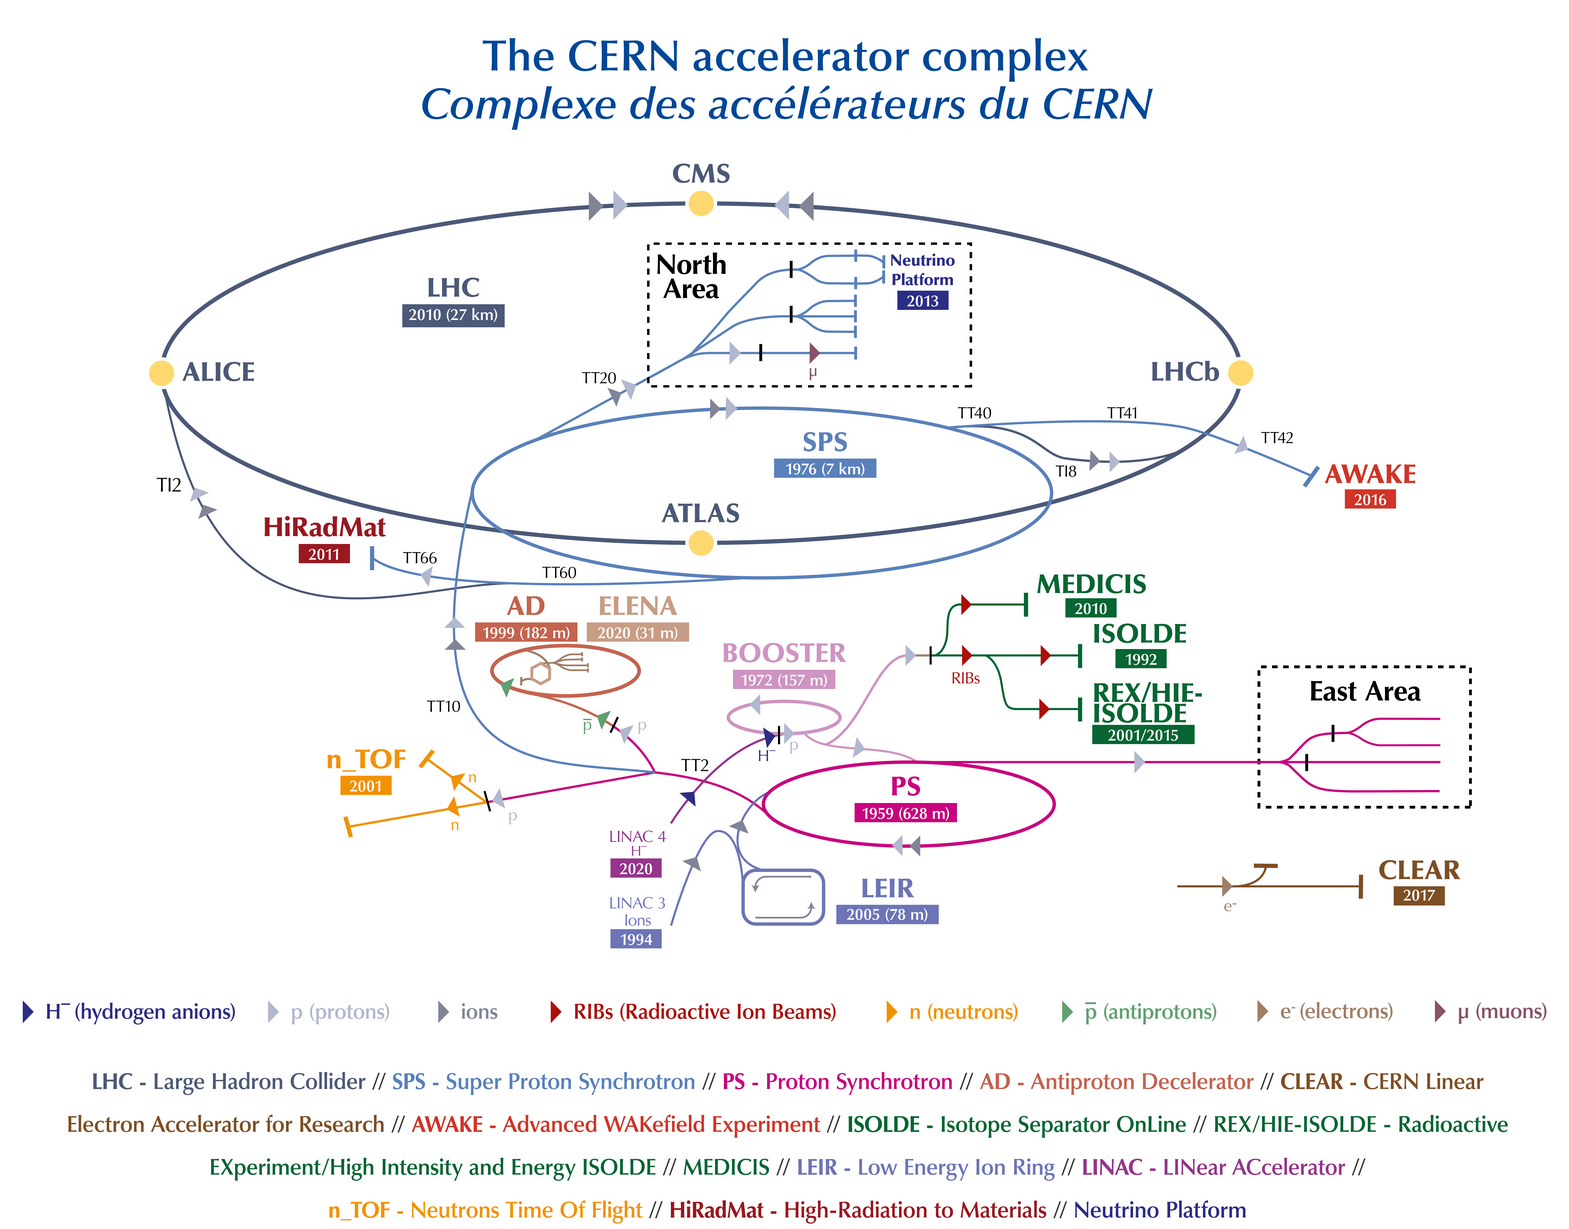
\includegraphics[width=0.99\textwidth]{Figures/cern_atlas/complex.png}
    \caption{The layout of the CERN accelerator complex as of 2022~\cite{CERNAC}.}
    \label{fig:cern_accelerator_complex}
\end{figure}

\subsection{Coordinate Systems}

In collider experiments, the typical coordinate system places the origin at the nominal IP, which, for hermetic detectors like ATLAS, Alice, and CMS, is at the centre of the detector.
The coordinate systems used by these experiments are right-handed, as shown in \Cref{fig:atlas_coordinate_system}, with the $z$-axis points along the beamline, the $y$-axis pointing upwards, and the $x$-axis pointing towards the centre of the LHC ring.
The transverse plane is defined as the plane perpendicular to the beam axis and is spanned by the $x$ and $y$ coordinates.

A polar representation is also often used, where the azimuthal angle $\phi$ is measured in the transverse plane from the $x$-axis, and the polar angle $\theta$ is measured from the $z$-axis.
The polar angle is frequently replaced with pseudorapidity $\eta$, defined as
\begin{equation}
    \eta = -\ln \left( \tan \left( \frac{\theta}{2} \right) \right).
\end{equation}
Differences in pseudorapidity are Lorentz invariant under boosts in the direction of the beamline, making it a useful quantity for describing the products of high-energy collisions.

Angular distances between objects are often measured in $\Delta R = \sqrt{(\Delta \eta)^2 + (\Delta \phi)^2}$, where $\Delta \eta$ and $\Delta \phi$ are the differences in pseudorapidity and azimuthal angle.
For collision products, a key observable is a transverse momentum $\pt=\sqrt{p_x^2 + p_y^2}$, where $p_x$ and $p_y$ are the components of the momentum in the transverse plane.

\begin{figure}
    \centering
    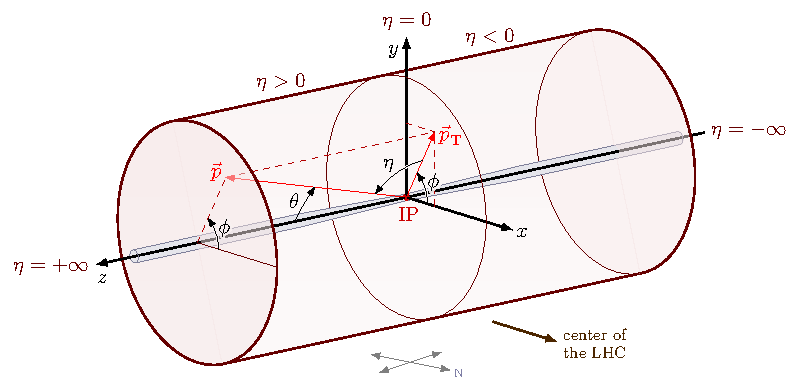
\includegraphics[width=0.6\textwidth]{Feynman/coordinate.pdf}
    \caption{The right-handed coordinate system used by the ATLAS experiment.}
    \label{fig:atlas_coordinate_system}
\end{figure}

\subsection{Cross-Section and Luminosity}

The cross-section, denoted by $\sigma$, indicates the likelihood of an interaction between two colliding particles.
Although calculating the cross-section involves quantum mechanical transition matrix elements and phase space integrals, it can be likened to the effective cross-sectional area of the particles participating in the interaction.

The total number of interactions $N$ depends on the cross-section of the process $\sigma$ and the integrated luminosity $L_{\text{int}}$ by the formula,
\begin{equation}
    N = \sigma L_{\text{int}} = \sigma \int \mathcal{L}(t) dt,
\end{equation}
where $\mathcal{L}(t)$ is the instantaneous luminosity.
This measures how tightly packed colliding particles are in a unit of space and time.
For two colliding beams with Gaussian densities, the instantaneous luminosity is given by
\begin{equation}
    \mathcal{L}(t) = \frac{N_1 N_2 f}{4 \pi \sigma_x \sigma_y} S(\theta_c),
\end{equation}
where $N_1$ and $N_2$ are the number of particles in each beam, $f$ is the frequency of bunch crossings, $\sigma_x$ and $\sigma_y$ are the root-mean-square beam widths in the $x$ and $y$ directions, and $S(\theta_c)$ is the geometric reduction factor due to the crossing angle $\theta_c$.
This last factor exists because the beams do not collide head-on, as this would result in multiple collision points, so they are crossed at a finite angle $\theta_c$.
This reduces the overlap of the beams when they pass through one another, reducing the effective luminosity.
For the $pp$ collisions at the LHC $S(\theta_c)$ is approximately $0.61$.
Even with this finite angle, long-range beam-beam interactions can still occur and must be accounted for.

The LHC was designed to deliver $\mathcal{L}(t) = 10^{34}~\unit{\centi\meter^{-2}\second^{-1}}$ at the IPs of ATLAS and CMS.
However, this has not been constant over the years, and each experiment independently measures the luminosity using well-understood processes.
The total integrated luminosity delivered by the LHC and recorded by ATLAS is shown in \Cref{fig:luminosity}.
The LHC's instantaneous luminosity has increased with each run and this is particularly beneficial for measurements on rare events where the uncertainty is statistically limited.

\begin{figure}
    \centering
    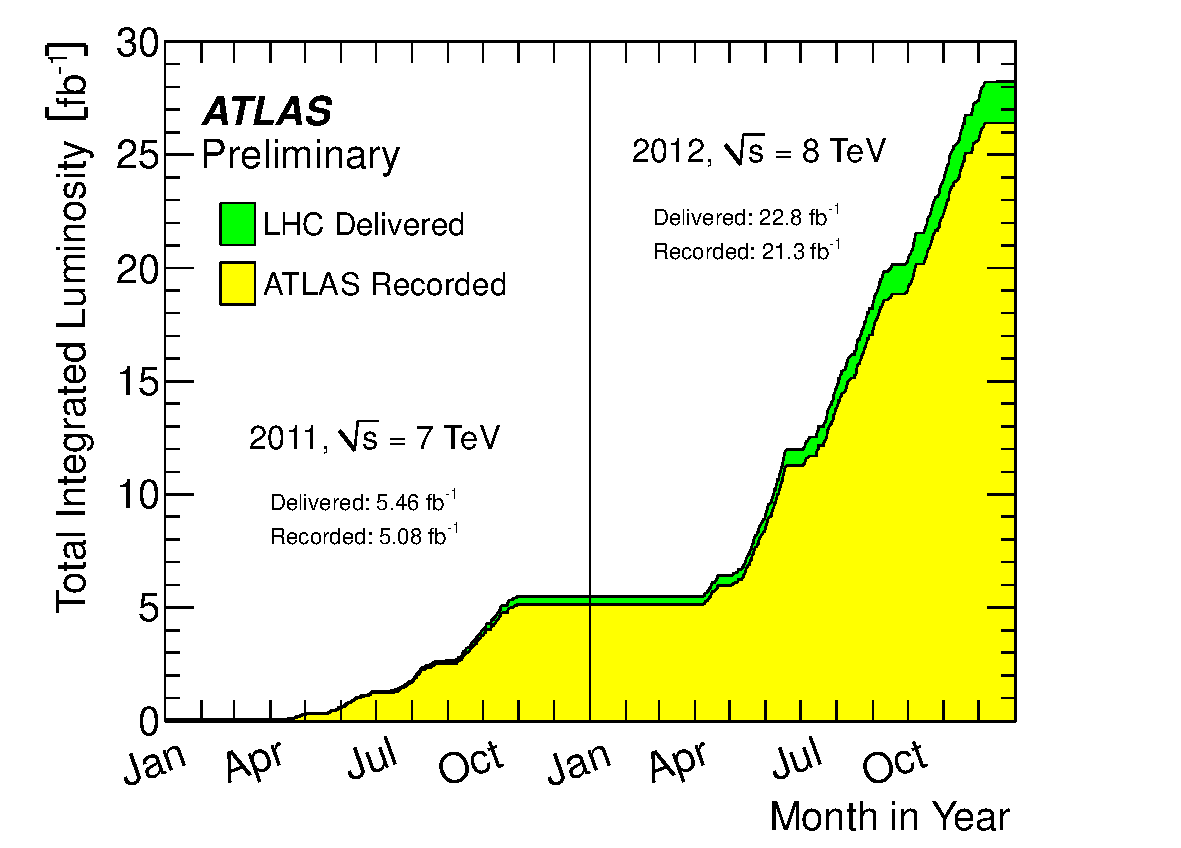
\includegraphics[width=0.32\textwidth]{Figures/cern_atlas/lumi1.pdf}
    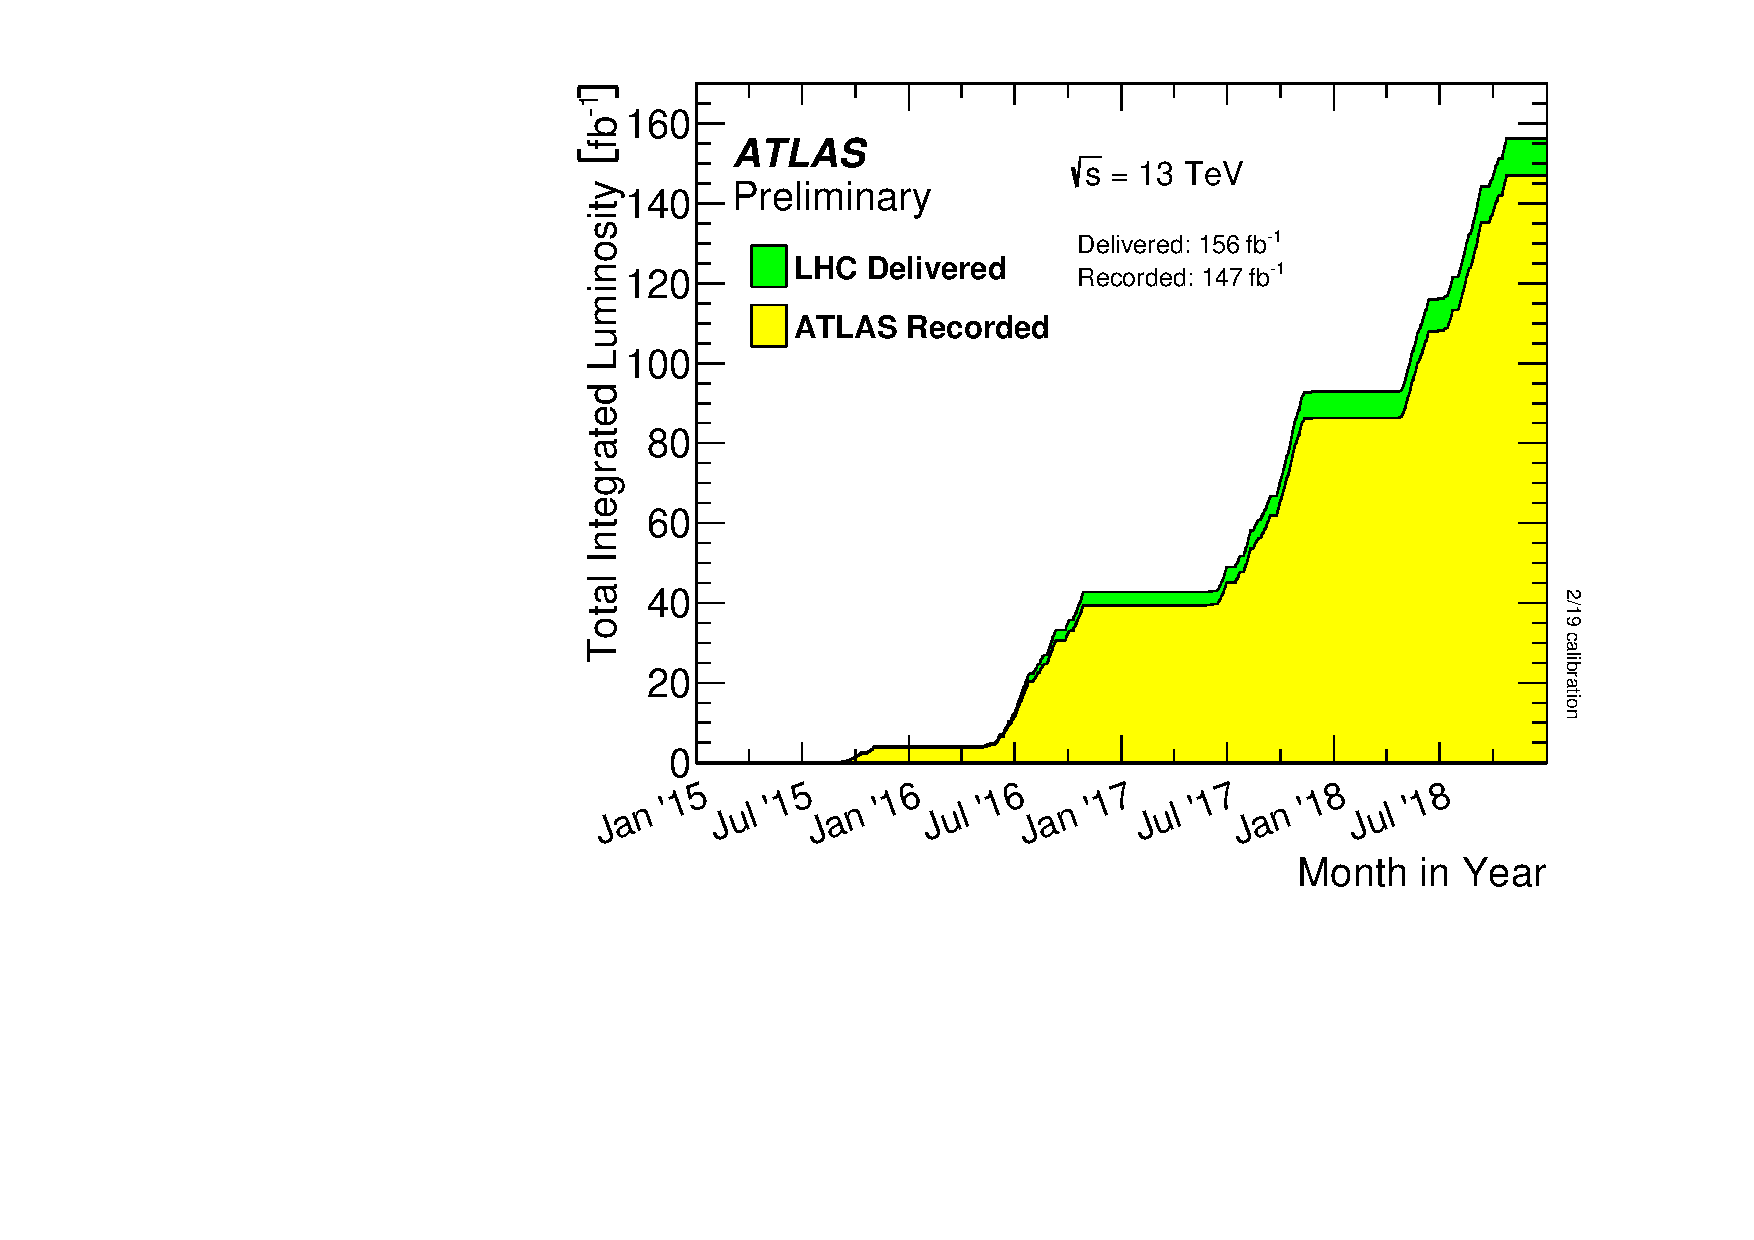
\includegraphics[width=0.32\textwidth]{Figures/cern_atlas/lumi2.pdf}
    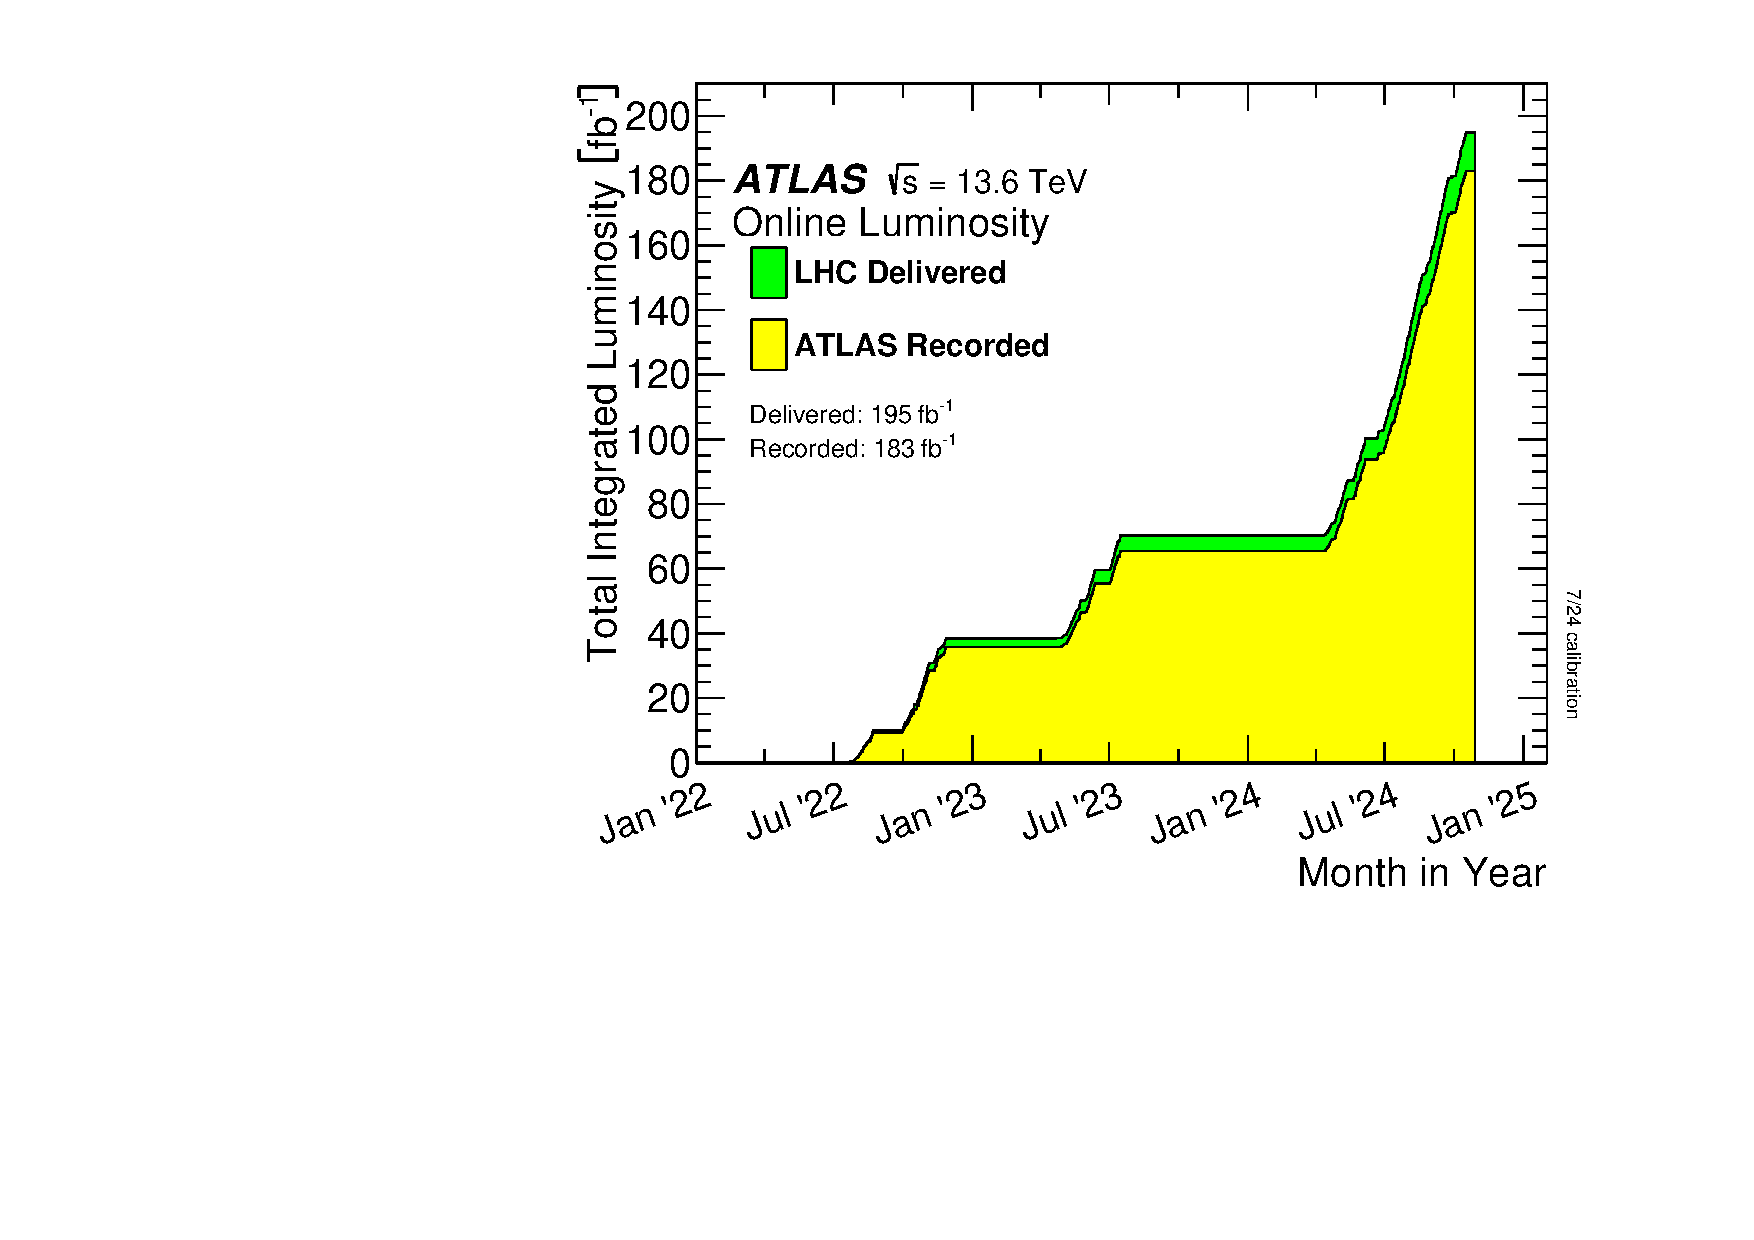
\includegraphics[width=0.32\textwidth]{Figures/cern_atlas/lumi3.pdf}
    \caption{The total integrated luminosity delivered by the LHC and recorded by the ATLAS experiment for Run 1 (left)~\cite{run1data}, Run 2 (middle)~\cite{run2data}, and Run 3 (right)~\cite{run3data}.}
    \label{fig:luminosity}
\end{figure}

\subsection{Pileup}

The increase in luminosity between Run 1 and Run 3 was in part achieved by raising the number of protons per bunch.
This in turn leads to more particle interactions per bunch crossing.
One of the undesirable effects of this is the large amount of overlapping signals in the detector which can degrade the resolution and efficiency of reconstruction algorithms.

Each bunch crossing in the collider generates a distinct event for analysis.
While the average number of interactions per crossing has increased with each LHC run, \Cref{fig:pileup} shows a wide distribution of interaction counts within each run.
Generally, only one of these interactions -- the hard scatter -- produces the high-energy particles captured by the detector and thus is of primary interest.
The remaining ``soft scatters'' are low-energy interactions that are known as in-time pileup.
Detector materials have a response and reset time, which can lead to residual signals from previous crossing being rerecorded, this is known as out-of-time pileup.
Filtering out signals from all pileup sources is crucial for accurate data analysis and poses a significant challenge as the LHC's luminosity increases.

\begin{figure}
    \centering
    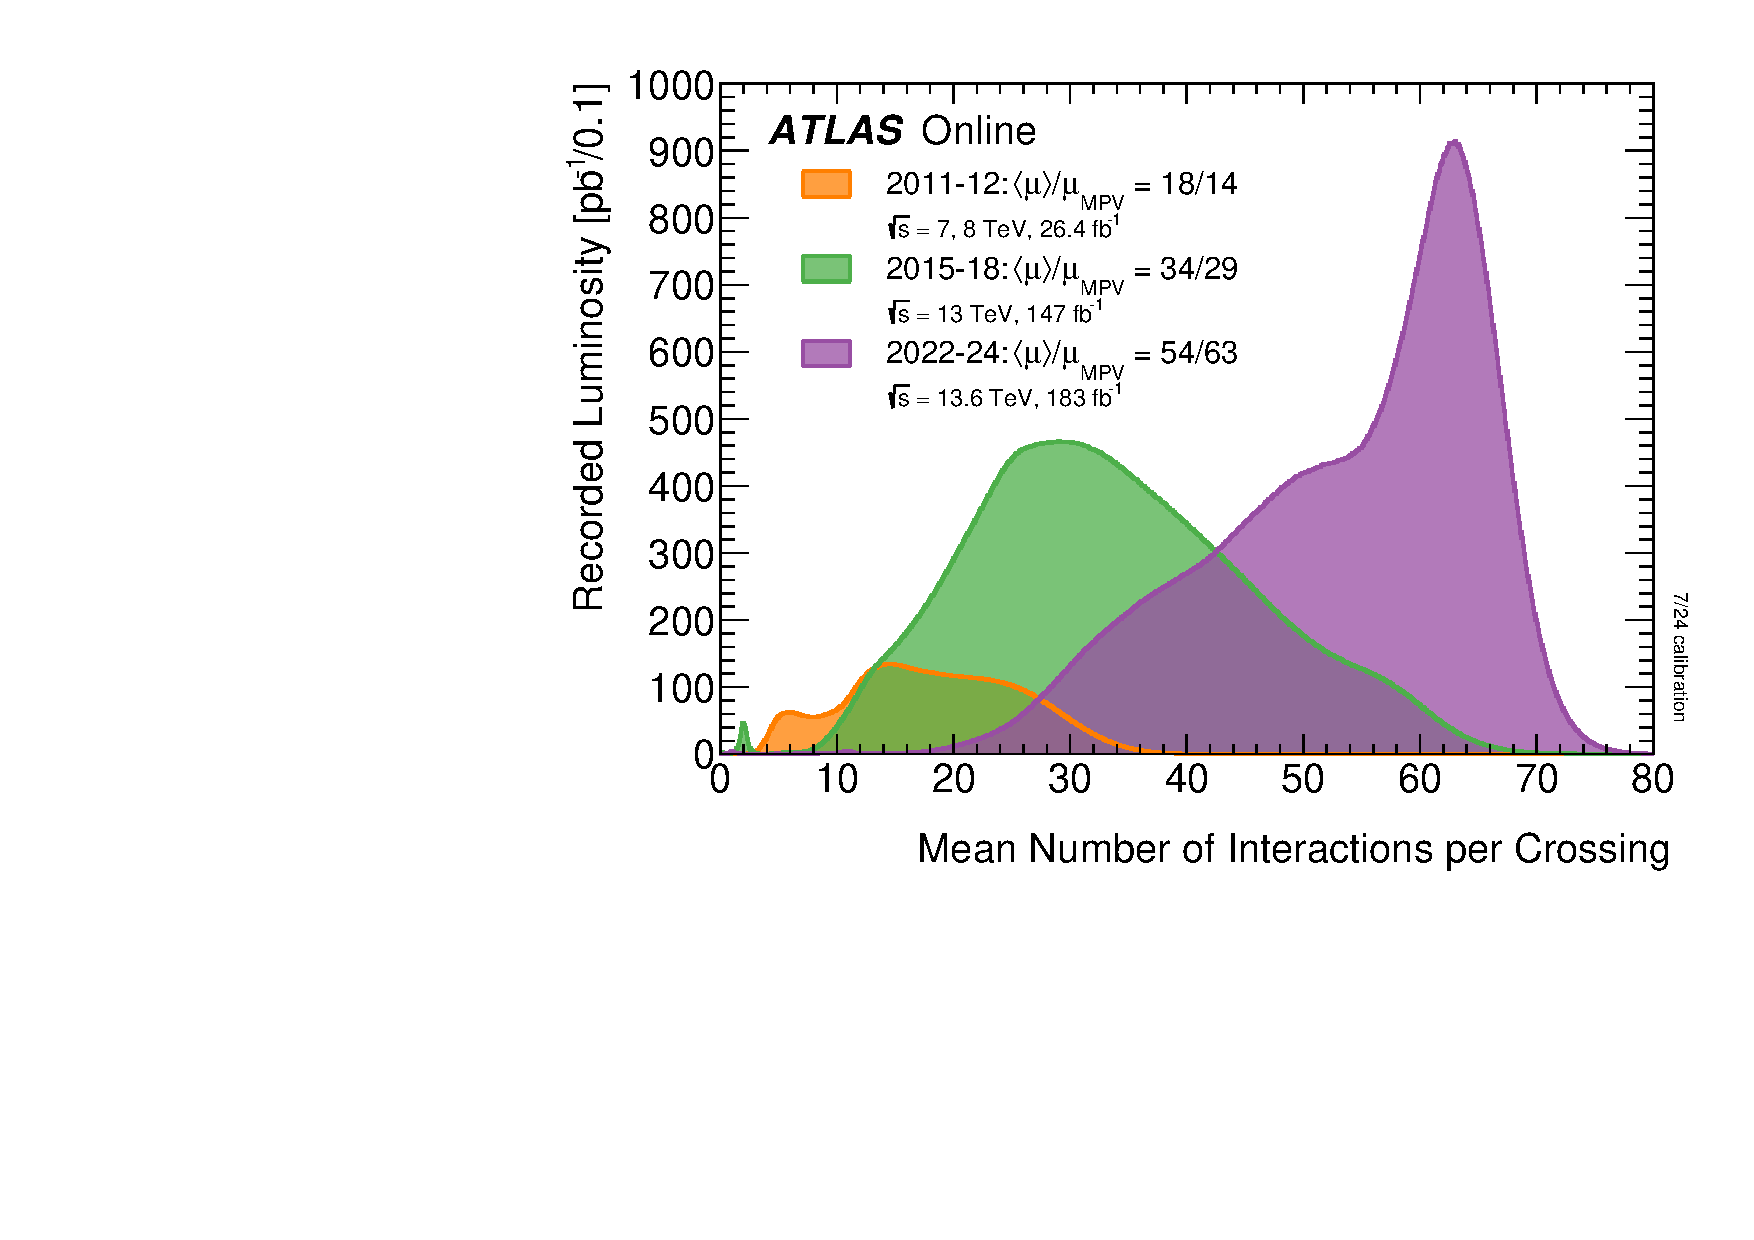
\includegraphics[width=0.6\textwidth]{Figures/cern_atlas/mu_run123.pdf}
    \caption{The distribution of the number of interactions per bunch crossing over the three LHC runs as measured by the ATLAS experiment~\cite{run3data}.}
    \label{fig:pileup}
\end{figure}

\subsection{LHC Runs}

The LHC operates on multi-year runs, the first beginning in 2010.
In between each run is a period of \textit{long-shutdown}, allowing for maintenance and upgrades to both the accelerator and the experiments.
The various run properties are shown in \Cref{tab:lhc_runs}.
Due to an electrical fault damaging many of the superconducting magnets in 2008, Run 1 was much delayed and operated at a reduced $\sqrt{s}=7~\TeV$ using a sparse bunch structure, only colliding at $20~\MHz$.
In 2012, the energy was increased to $\sqrt{s}=8~\TeV$.
The total delivered luminosity of the run was $28.4~\ifb$.
Run 2 spanned from 2015 to 2018, with an increased energy of $\sqrt{s}=13~\TeV$, a bunch crossing rate of $40~\MHz$, and a total integrated luminosity of $156~\ifb$.
Run 3 began in 2022 and is expected to continue until 2026 and has already surpassed Run 2 with $195~\ifb$ of data delivered~\cite{run3data}.

\begin{table}[h!]
    \centering
    \caption{Overview of the different LHC runs~\cite{LHCRun2,LHCRun3,run1data, run2data, run3data}. Values for Run 3 are preliminary as data is still being collected.}
    \label{tab:lhc_runs}
    \resizebox{\textwidth}{!}{
        \begin{tabular}{lcccccc}
            \toprule
                              & $\sqrt{s}~[\TeV]$ & $\mathcal{L}_\text{int}~[\ifb]$ & Protons per bunch     & Bunch spacing $[\ns]$ & \avemu \\
            \midrule
            Run 1 (2010-2011) & 7                 & 5.5                             & $1.45 \times 10^{11}$ & 50                    & 10     \\
            Run 1 (2012)      & 8                 & 22.8                            & $1.6 \times 10^{11}$  & 50                    & 21     \\
            Run 2 (2015-2028) & 13                & 156                             & $1.25 \times 10^{11}$ & 25                    & 34     \\
            Run 3 (2022-)     & 13.6              & 195                             & $1.8 \times 10^{11}$  & 25                    & 50     \\
            \bottomrule
        \end{tabular}
    }
\end{table}

\section{The ATLAS Experiment}

The ATLAS experiment~\cite{ATLAS, ATLASRun3} is one of the four primary experiments at the LHC\@.
It is the largest particle detector of the four, weighing $7000$ tonnes and measuring $44$ m long and $25$ m in diameter.
It is a general-purpose detector designed to explore a wide range of physics phenomena.
To achieve this, it has multiple sub-detectors designed to capture a broad range of outgoing products from the $pp$ collisions.
The ATLAS detector is shown in \Cref{fig:atlas_detector}.

The detector is hermetic, meaning it covers nearly the entire solid angle of $4\pi$.
It is arranged in concentric cylindrical-like layers around the IP\@.
Each layer contains a barrel region, which wraps around the beamline, and end-cap regions, which cover the flat edges of the cylinder on either side.

This section describes the ATLAS detector, focusing on the tracking systems.
These systems provide precise position and momentum measurements of charged particles, which are used to reconstruct particle trajectories and vertices.

\begin{figure}[htb]
    \centering
    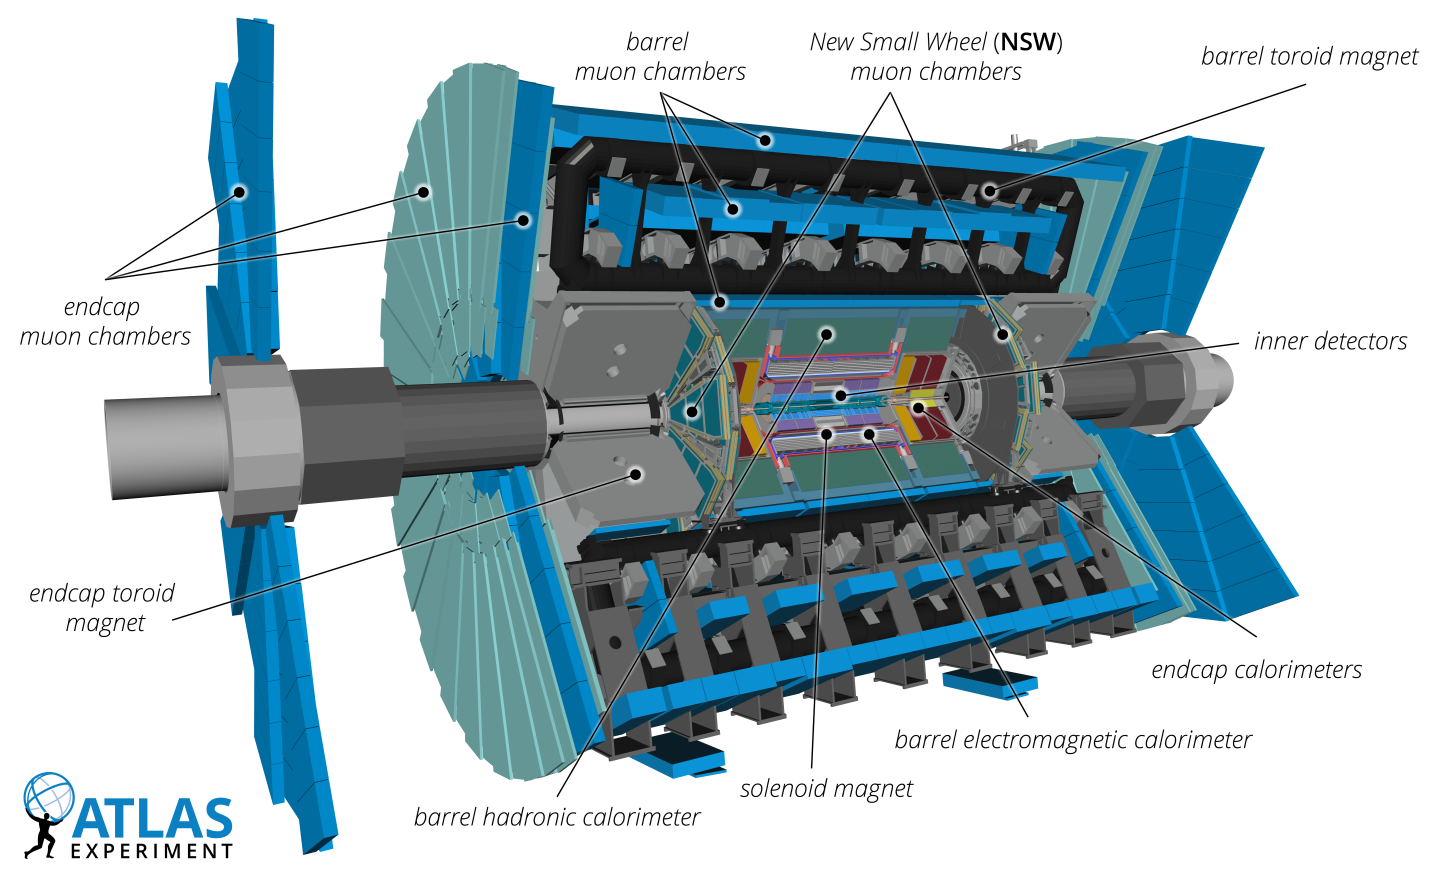
\includegraphics[width=0.99\textwidth]{Figures/cern_atlas/ATLAS.png}
    \caption{The ATLAS detector at the LHC\@. Image taken from Ref.~\cite{ATLASRun3}.}
    \label{fig:atlas_detector}
\end{figure}

\subsection{Inner Detector}

The Inner Detector (ID) is the innermost sub-detector of ATLAS and is shown in \Cref{fig:atlas_inner_detector}.
It comprises three sub-detectors: the Pixel Detector, the Semi-Conductor Tracker (SCT), and the Transition Radiation Tracker (TRT).
It is designed to capture charged particle signals with a pseudorapidity $|\eta| < 2.5$.
These signals are clustered into points in space where the particles have ionized the detector material.
These points can be used to reconstruct the charged particle's trajectory -- track -- as it propagates out from the centre of the detector.

The ID is immersed in a $2~\tesla$ axial magnetic field generated by a 5.8 m long superconducting solenoid magnet containing over $9\km$ of NbTi wire.
The magnetic field causes the particles to bend in a plane perpendicular to the beamline, tracing out a helical path whose curvature is proportional to $q/p$, where $q$ is the charge of the particle and $p$ is the magnitude of its momentum.

A fully reconstructed track is characterized by five parameters, which are shown in \Cref{fig:track_parameters}.
These include the charge-to-momentum ratio $q/p$, the azimuthal angle $\phi$, the polar angle $\theta$.
By tracing the track back to the beamline, the longitudinal $z_0$ and transverse $d_0$ impact parameters are determined at the point of closest approach to the IP\@.
These impact parameters represent the distances measured in each respective direction.
The relative $\pt$ resolution of the ID is described as,
\begin{equation}
    \sigma(\frac{1}{\pt}) = 0.36 \oplus \frac{13}{\pt \sin(\theta)}~\TeV
\end{equation}
where $\oplus$ denotes a sum in quadrature.

\begin{figure}[htb]
    \centering
    \includegraphics[width=0.6\textwidth]{Figures/cern_atlas/Track.png}
    \caption{The main parameters of a reconstructed track in the ATLAS Inner Detector. Image taken from Ref.~\cite{ATLASTrackingSoftware}.}
    \label{fig:track_parameters}
\end{figure}

\begin{figure}[htb]
    \centering
    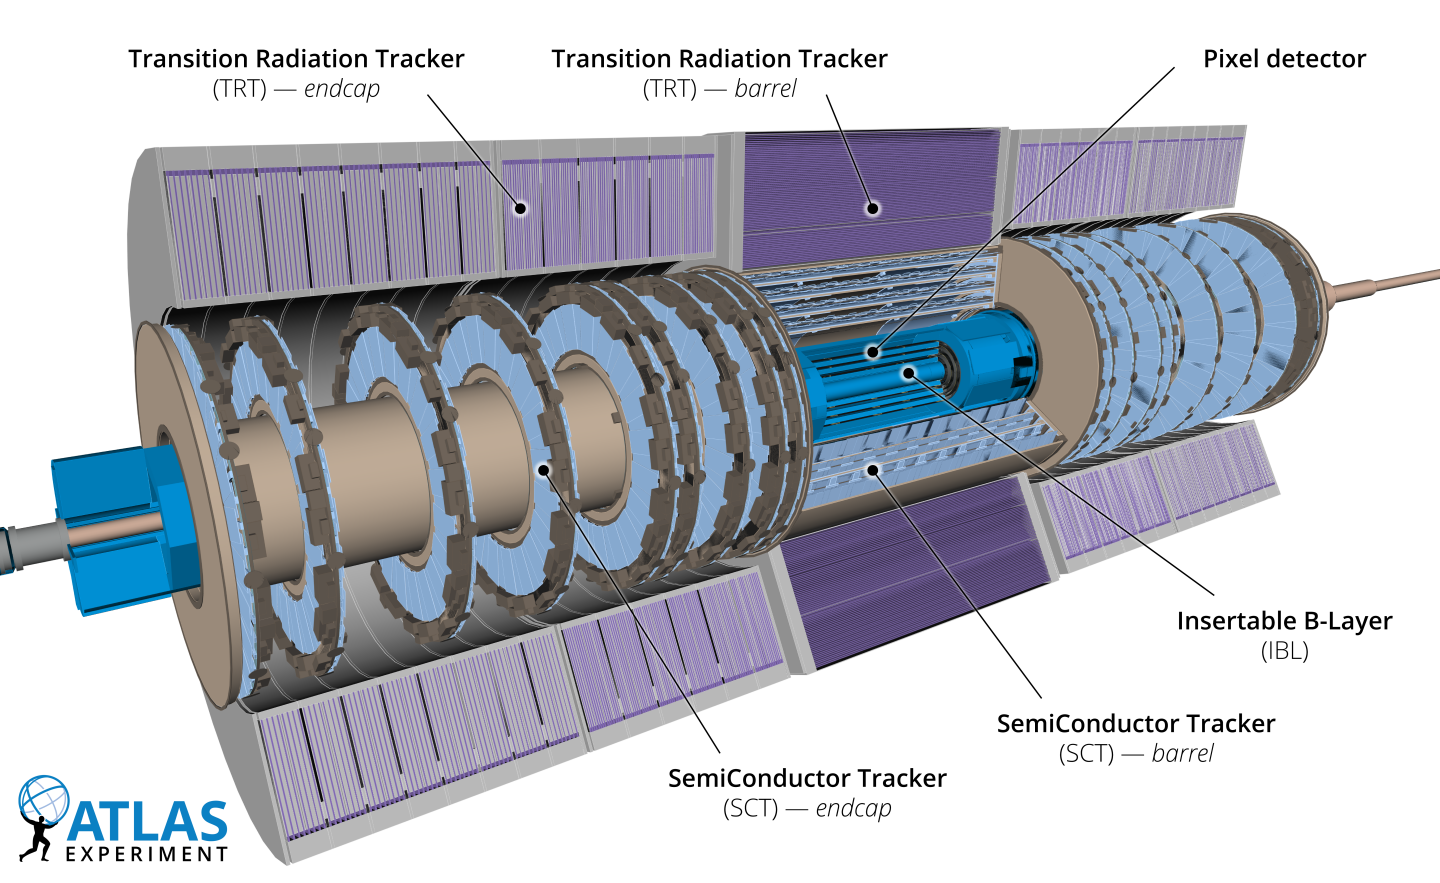
\includegraphics[width=0.59\textwidth]{Figures/cern_atlas/BetterID.png}
    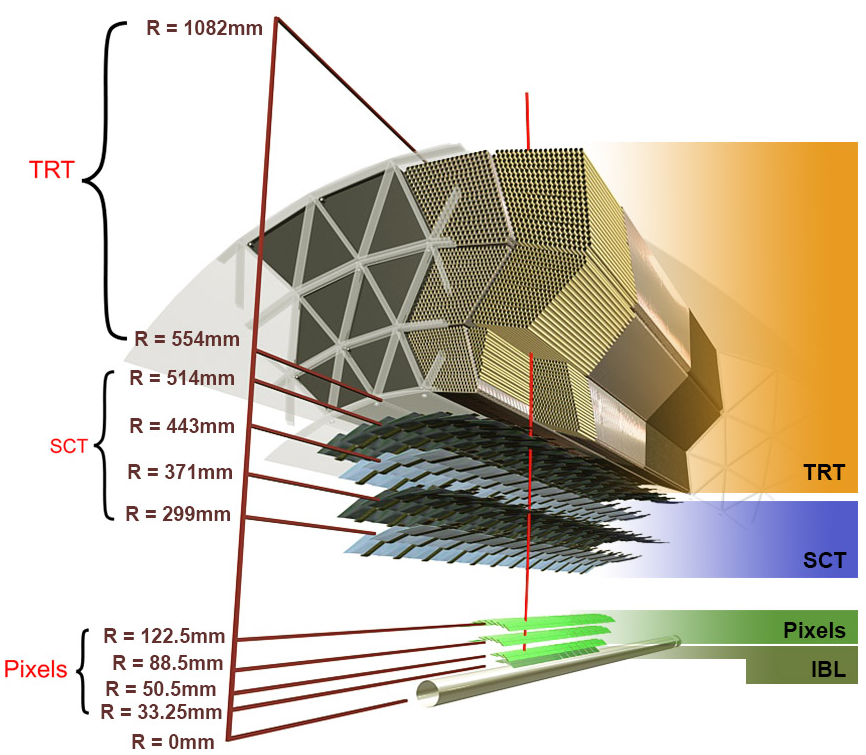
\includegraphics[width=0.39\textwidth]{Figures/cern_atlas/IDCut.png}
    \caption{Schematic of the full ATLAS Inner Detector (left) and a cross-section of the barrel region (right). Images taken from Refs.~\cite{ATLASRun3,IBLPhotos}.}
    \label{fig:atlas_inner_detector}

\end{figure}

\subsubsection{Pixel Detector}

The high-granularity silicon pixel detector~\cite{ATLASPixel} covers the innermost region of the ID.
It measures 1.4 m long and is fully contained in a diameter of 0.5 m.
High granularity is required at this scale to resolve the numerous tracks that pass through it.
Individual silicon pixels are about $50~\um$ wide in the transverse direction and about $400~\um$ long in the longitudinal direction.

Each pixel has a slight potential difference applied across it.
Ionizing radiation left by a traversing charged particle generates electron-hole pairs that drift and are collected at the p-n junctions, providing a signal.
The pixel detector has 1744 modules, each containing around 46k pixels, resulting in 80M readout channels.
These are arranged in three barrel layers placed at a radius of $50.5~\mm$, $88.5~\mm$, and $122.5~\mm$ from the beamline, with four end-cap disks on each side.

Between Run 1 and 2, an additional layer was added at a radius of $33~\mm$ to the beamline, known as the Insertable B-Layer (IBL)~\cite{ATLASIBL}.
Pixels in the IBL measure $50~\um$ in the transverse direction and $250~\um$ in the longitudinal direction.
This layer improved the $\pt$ resolution of the detector by close to 30\% for low $\pt$ tracks.
Furthermore, the enhanced $z$-resolution improved impact parameter resolution and cluster separation, allowing for better reconstruction of primary and secondary vertices.

\subsubsection{Semiconductor Tracker}

The Semiconductor Tracker (SCT)~\cite{ATLASSCT} surrounds the Pixel Detector, occupying the region between $299~\mm$ and $514~\mm$ from the beamline.
It comprises four concentric barrel layers with nine disks at each end-cap covering the region $|\eta| < 2.5$.
Like the pixel detector, the SCT is composed of silicon readout channels. Unlike the pixels, each microstrip measures $20~\um \times 12~\cm$ and thus only has high granularity in a single direction, oriented to the transverse momentum.
To improve longitudinal resolution, each SCT layer includes two back-to-back microstrip layers, rotated by $40 \unit{\milli\radian}$ relative to each other.
The SCT in total has around 6.3M readout channels.

\subsubsection{TRT}

The outermost sub-detector of the ID is the Transition Radiation Tracker (TRT)~\cite{ATLASTRT}.
It is a straw-tube tracker that aids in the momentum measurement and provides information for particle identification for tracks within $|\eta| < 2.0$.
The TRT provides the most hits per track, around 35 on average, of the three sub-detectors.
At a greater distance from the beamline, it also does not require such fine spatial resolution as the silicon detectors to provide a good measurement of the track kinematics.

It comprises approximately 300k thin-walled drift tubes, each $4~\mm$ in diameter
The barrel region contains 50k tubes, each $144~\cm$ long, while the end caps contain 250k tubes, each $37~\cm$ long.
A potential difference exists between the tube walls and an axial wire.
When a charged particle intersects the tube, it ionizes the predominantly argon gas inside, and the resulting electrons drift towards the wire, providing the signal.
There is no information on where the ionization occurred along the length of the tube.
Thus, resolution for the barrel region is only defined in the $r-\phi$ plane, and for the end-cap, it is only defined for $z-\phi$.
A polymer foil is placed between the tubes to generate transition radiation, the pattern of which allows discriminating between electrons and pions.

\subsection{Calorimeters}

ATLAS has three calorimeter systems outside the central solenoid magnet, which measure the energies of particles produced by the collisions.
Each calorimeter is designed with alternating layers of absorber and active materials.
Particles interact with the absorbers, lose energy, and produce showers of secondary particles that ionize the active material, which can be converted into a measurable signal.
These layers are typically arranged in an accordion-like structure to ensure homogenous coverage.
Different absorber materials are used to optimize the interaction and thus containment of the showers for different particle types.

The Electromagnetic Calorimeter (ECal) is specialized for measuring the energies of electrons and photons.
Surrounding this is the Hadronic Calorimeter (HCal), which is designed to measure the energies of hadrons.
These subsystems cover the region $|\eta| < 3.2$.
In addition, there is also the forward calorimeter subsystem, which measures the energy of particles in the range $3.2 < |\eta| < 4.9$.
However, information from this subsystem is not used in this work, and it is omitted from the following descriptions.
A schematic of the calorimeter systems is shown in \Cref{fig:atlas_calorimeters}.

\begin{figure}[htb]
    \centering
    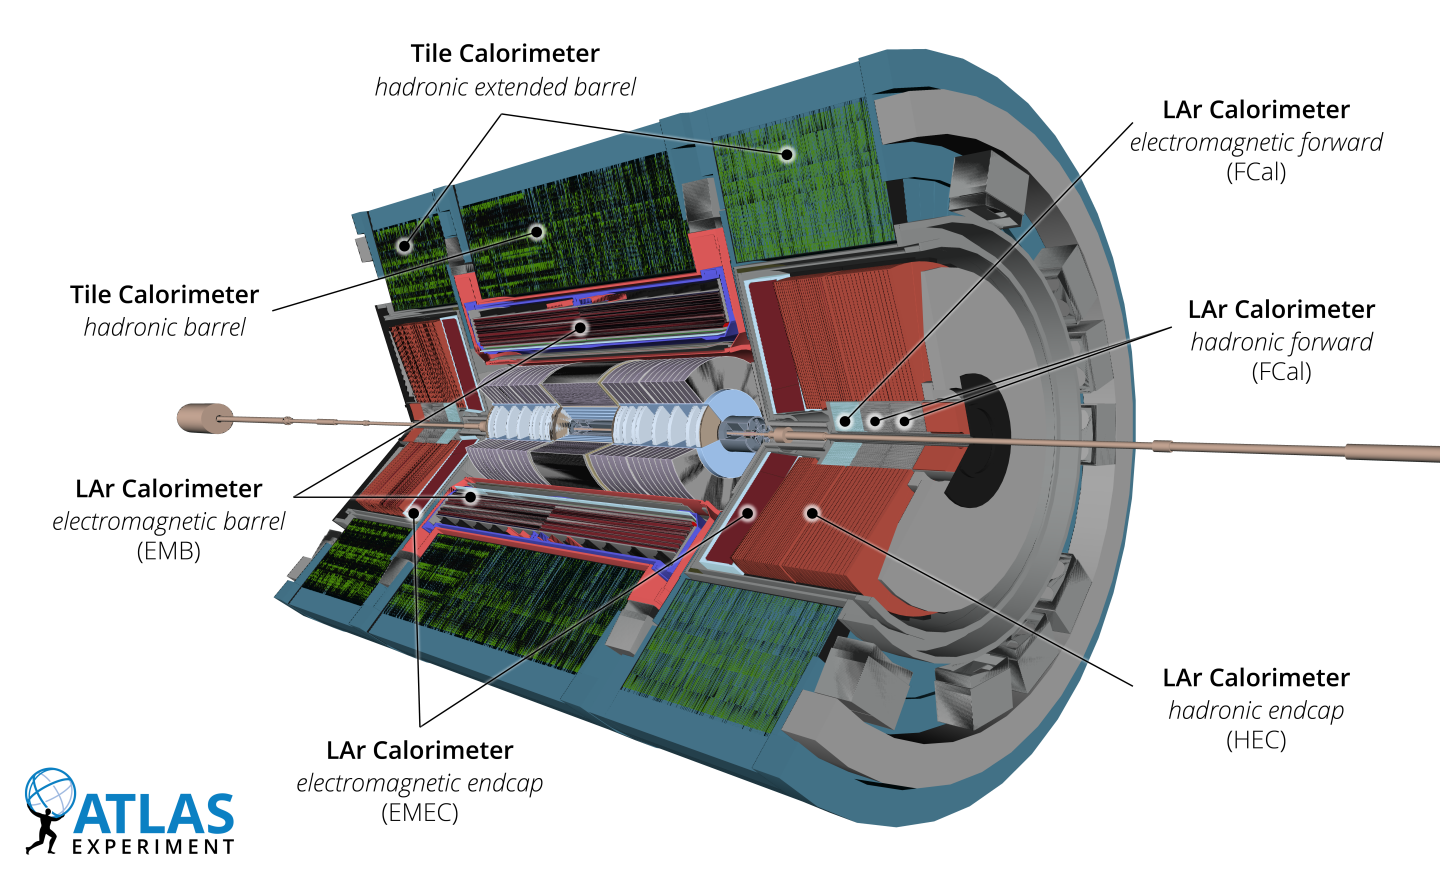
\includegraphics[width=0.99\textwidth]{Figures/cern_atlas/Calos.png}
    \caption{Schematic of the ATLAS calorimeter systems. Image taken from Ref.~\cite{ATLASRun3}.}
    \label{fig:atlas_calorimeters}
\end{figure}

\subsubsection{Electromagnetic Calorimeter}

The Cal~\cite{ATLASECal} is a high granularity calorimeter which uses liquid argon as the active material and lead as the absorber.
To keep the argon in a liquid state, the ECal is cooled to $-185~\unit{\degree C}$.
These materials are chosen to optimize the containment of electromagnetic showers produced by electrons and photons, via pair production and bremsstrahlung radiation, while minimising the energy loss of heavier particles.
The barrel ECal covers the range $|\eta| < 1.475$ and is split into three layers, decreasing in granularity with distance from the beamline.
The inner layer allows for more precise shower measurements which assists in the identification of pions.
The Liquid Argon Electromagnetic Enc-Cape (EMEC) and covers the range $1.375 < |\eta| < 3.2$.
Unlike the ID, the ECal resolution increases with incident particle energy.

\subsubsection{Hadronic Calorimeter}

The HCal or Tile Calorimeter~\cite{ATLASHCal} encompasses the ECal and is designed to measure the energies of hadrons.
It uses steel as the absorber and scintillating tiles as the active material made from polystyrene.
The hadrons are contained by losing energy through inelastic nuclear interactions with the steel, producing a shower of electrons and photons which are detected by the tiles.
In the forward regions of the calorimeter, $1.5 < |\eta| < 3.2$, a copper/LAr combination is used.
The granularity and energy resolution of the HCal are lower than the ECal.

\subsection{Muon Spectrometer}

Other than neutrinos, which traverse the entire detector without interacting, muons are the only particles that easily penetrate through the calorimeters, incurring minimal energy loss.
Though they leave tracks in the ID, the Muon Spectrometer (MS)~\cite{ATLASMuon,ATLASRun3} provides triggering information, identification, and extra momentum measurements for muons.
The MS is the outermost sub-detector of ATLAS and is shown in \Cref{fig:atlas_muon_spectrometer}.
Its systems are arranged in three barrel layers covering $|\eta| < 1.2$ and several end-cap layers or wheels covering $1 < |\eta| < 2.7$.
The wheels are placed on either side of the detector at a distance of $7.4$~m, $14$~m, and $21.5$~m from the IP.

Monitored Drift Tubes are the spectrometer's primary tracking component and are similar in principle to the straw tubes in the TRT@.
More than 380k aluminum tubes, each with a diameter of $30$~mm and primarily filled with argon gas, are organized into three barrel layers and four end-cap disks.
In addition, Cathode Strip Chambers are used in inner layers of the end-cap to cope with the higher particle flux.
These are multi-wire proportional chambers built into strips.

Three large air-core toroidal magnets generate the magnetic field in the MS\@, one in the barrel region and one in each end-cap regions.
Each magnet has eight coils and deflects the muons, allowing for the measurement of their momentum.

\begin{figure}[htb]
    \centering
    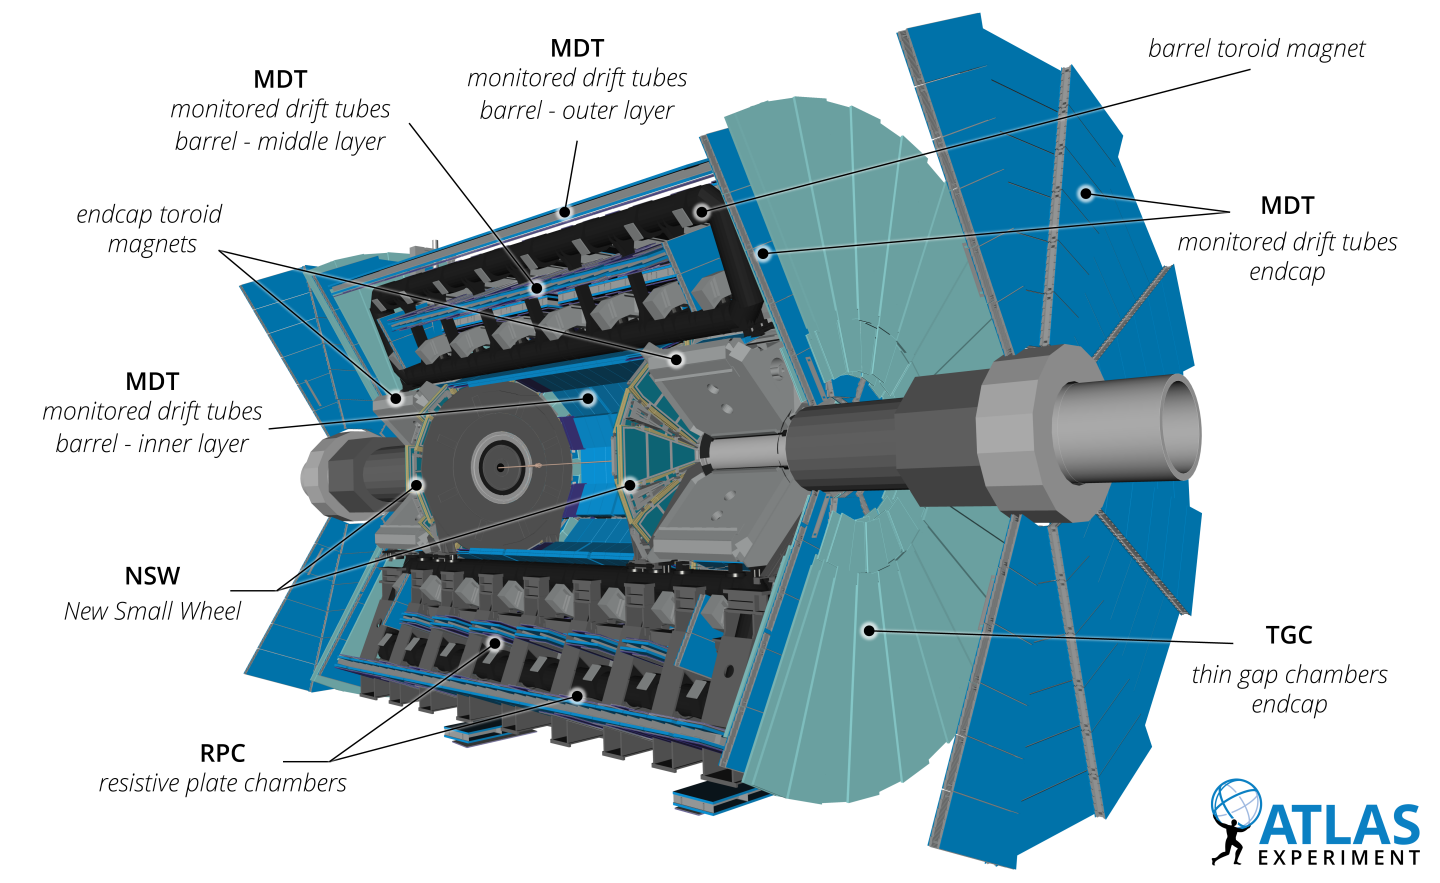
\includegraphics[width=0.99\textwidth]{Figures/cern_atlas/MS.png}
    \caption{Schematic of the ATLAS Muon Spectrometer. Image taken from Ref.~\cite{ATLASRun3}.}
    \label{fig:atlas_muon_spectrometer}
\end{figure}

\section{Reconstruction}
\label{sec:event_reconstruction}

Reconstruction is the process of converting the raw detector signals into collections of defined physical objects to better understand the collision events.
This process is performed offline, after the data has been recorded and stored, and uses information from all sub-detectors.

This section describes the basics of track, vertex, and jet reconstruction at ATLAS, as well as several approaches to jet tagging.

\subsection{Tracks}

Track reconstruction refers to taking the collection of hits registered by the ID, and grouping them into individual tracks likely to have been produced by a single charged particle.
Tracks are key ingredients in the reconstruction and identification of other particles, such as electrons and muons, jets, and the multiple vertices produced in each collision.
A full description of the track reconstruction pipeline used for ATLAS Run 2 data can be found in Ref.~\cite{PerformanceATLASTrack}.
Track reconstruction is performed in nuerous stages.
Hits are first clustered into space points, after which iterative track-finding algorithms are used, followed by cleaning and ambiguity resolution.

\subsubsection{Clusterization}

A single particle may deposit energy in multiple adjacent pixels or strips in the ID\@.
This is due to the drift of electrons between sensors within the solenoid magnetic field or from the incident angle of the particle.
These hits are first combined into clusters which are then used to form \textit{space points} (SP) defined in three dimensions.
For the SCT, these clusters also combine information from the two back-to-back layers.
Position uncertainties of these points are estimated from cluster sizes and detector geometry.
In dense environments the clustering algorithm may merge mistakenly merge hits from different particles, leading to a higher rate of fake tracks.

\subsubsection{Track Seeding}

Tracks are \textit{seeded} by grouping triplets of SPs in three sequential layers in either the pixel or SCT subdetectors.
Each of these seeds forms a \textit{track candidate} and are used to determine the first crude estimates of the track parameters, assuming a perfectly uniform magnetic field and helical trajectory.
The only requirement to improve purity is that one additional SP is found compatible with the track candidate outside the seeding region.

A combinatorial Kalman filter~\cite{ApplicationKalmanFiltering} is employed to iteratively extend this candidate by incorporating additional SPs in the other layers both towards and away from the IP\@.
If multiple compatible space-point extensions are found on the same layer, the filter generates several track candidates for each seed.
At this stage, hits may be shared between multiple candidates, which is intentionally done to maximize the number of possible candidates and thus the efficiency of the algorithm.

The following steps are designed to improve the track quality and remove fake tracks.

\subsubsection{Ambiguity Resolution}

The ambiguity resolver begins by defining a \textit{track score} for each candidate.
This score quantifies the likelihood that each candidate corresponds to a real trajectory.
The score takes into account several factors; the number of SP assigned to the track will increase its score, while the number of holes will decrease it.
Holes are defined as intersections between the reconstructed track and active sensor material where no matching SP is found.
They can be found in data due to inefficiencies in the silicon sensors.
The track score also considers the $\chi^2$ of the track fit.
Tracks with higher \pt also receive a higher score.
The ambiguity resolver then iterates over the list of track candidates in order of decreasing score.

Clusters can overlap naturally in high-density environments.
These are referred to as \textit{merged clusters}.
A neural network estimates the number of particles traversing each cluster and their positions~\cite{NeuralNetworkClustering}.
This information allows the cluster to be split and allocated to the different candidates.
A track can have no more than two shared clusters, and clusters may be shared by no more than two tracks, with preference given to the track with the highest score.
The refined and purified track candidates are then re-fit to obtain the final parameters.
It obtains a new score and is inserted back into the list of candidates.

During this stage, seeds that fail the track-finding process are checked for compatibility with information from the calorimeter.
If a seed is within a region of interest in the calorimeter, the track-finding procedure is repeated, permitting an extra \textit{kink} in the track as this may have been caused by Bremsstrahlung radiation.
This step improves electron reconstruction efficiency.

The ambiguity resolver fully rejects track candidates if they fail to meet the criteria in \Cref{tab:track_criteria}.
If the track is processed twice by the resolver without modification, it is saved to the final collection and all associated hits are removed.

\begin{table}[h!]
    \centering
    \begin{tabular}{ll}
        \toprule
        Parameter           & Selection   \\
        \midrule
        $p_T$               & $> 400$ MeV \\
        $|\eta|$            & $< 2.5$     \\
        $|d_0|$             & $< 3.0$ mm  \\
        $|z_0 \sin \theta|$ & $< 5$ mm    \\
        Shared clusters     & $< 2$       \\
        SCT + Pixel hits    & $\geq 8$    \\
        Pixel holes         & $< 2$       \\
        SCT + Pixel holes   & $< 3$       \\
        \bottomrule
    \end{tabular}
    \caption{Track selection criteria used by the ambiguity resolver.}
    \label{tab:track_criteria}
\end{table}

\subsubsection{TRT Extension}

Finally, information from the TRT is used to extend the tracks.
A similar Kalman filter incorporates TRT hits starting from the predicted intersection between each silicon track and the TRT.
If successful, the TRT hits are added to the track, and the whole track is fit once more using a global $\chi^2$ fitter.
The inclusion of TRT hits enhances momentum resolution and allows for particle identification.
However, the extension may be rejected if it worsens the $\chi^2$ of the track candidate or if more than 50\% of the TRT hits are tube hits with no leading edge.

\subsection{Vertices}

Vertex reconstruction is the process of identifying the many primary and secondary vertices produced in each collision.
Each vertex is a location in space, constructed from a convergence of fully reconstructed tracks, and indicates the point of origin for multiple charged particles.

Primary vertices are those produced by the many $pp$ collisions during the bunch crossing.
For Run 1 and 2, the primary vertices are reconstructed using the Iterative Vertex Fitter~\cite{ATLASVertex}.
First, a seed position of the vertex is selected using the mode of the $z$-coordinate all tracks in the event measured at the point of closest approach to the beamline.
Next, the vertex position is iteratively refined, and in each iteration, less compatible tracks are down-weighted.
After the final iteration, all tracks with low enough weights are removed from the vertex and used for the next.

For each event, the primary vertex with the highest $\Sigma\pt^2$ of all associated tracks is labelled as the \textit{hard scatter vertex}.
It is sometimes ambiguously referred to as \textit{the} primary vertex (PV) while the others are referred to as \textit{pileup} vertices.
Reconstruction on Run 3 data is switching to an Adaptive Multi-Vertex Fitter~\cite{Run3Vertex}.

Secondary vertices are those produced by the decay of particles originating from the PV.
This secondary decay must take place at a distance sufficiently far away in the transverse plane to be resolved and not mistakenly identified as pileup.
They are typically caused by the decay of long-lived $b$-hadrons or the interaction of particles with the detector material and are thus crucial tools for identifying $b$-jets.
In ATLAS, secondary vertex reconstruction is performed within the context of jet reconstruction using the JetFitter~\cite{JetFitter} or SV1~\cite{SV1} algorithms.

\subsection{Jets}
\label{sec:jets_reconstruction}

As described in \Cref{sec:jets} are an emergent property of QCD\@, which results in a collimated spray of particles stemming from the decay and fragmentation of an initiating color-charged parton.
From a detector perspective, jets result in large localized energy deposits in both calorimeters and many tightly packed tracks in a cone emanating from the PV.
The width of the jet cone is dependent on the mass of the initiating particle and its transverse momentum, with $\Delta R \approx \sfrac{2m}{\pt}$.

Due to the stochastic nature of the showering process, the jet signal can never be perfectly isolated.
Particles within the jet cone may overlap with other initial state radiation, multiple parton interactions (from the underlying event), or pileup.
Jet reconstruction is, therefore, a difficult optimization problem.
The goal is to maximally capture the energy of the initiating particle while minimizing the contamination from other sources.
A jet reconstruction algorithm should capture all hard partons in the event, have an axis parallel to the jet momentum, and accept roughly uniform contamination.

Jet reconstruction in ATLAS is performed using the anti-$k_t$ algorithm~\cite{AntiKt}.
This is a sequential recombination algorithm that iteratively clusters a collection of objects.
It is both infrared and collinear safe.
The algorithm is defined by a maximum distance parameter $R$.
The algorithm begins with the hardest, highest \pt, object in the event $i$.
During each iteration, the distance $d_{ij}$ is calculated to all other objects $j$ in the event,
\begin{equation}
    d_{ij} = \frac{1}{\max(\pt{_i}^2, \pt{_j}^2)} \frac{\Delta R_{ij}^2}{R^2}.
\end{equation}
If this value is less than $\sfrac{1}{\pt{_i}^2}$, then the objects are combined, and the algorithm proceeds; otherwise, $i$ is considered a jet and removed from the list.
The algorithm continues until all objects are clustered or declared as jets.

Jets can be clustered using the anti-$k_t$ algorithm with a variety of inputs.
During Run 1, jets were constructed from topo-clusters, topologically connected calorimeter cells~\cite{TopoJets}.
In some analyses, jets are clustered from tracks only~\cite{TrackJets}.
The general approach for Run 2 and 3 data is to include both sets of information using the Particle Flow (PFlow) algorithm~\cite{PFlow}.

\subsubsection{Particle Flow}

The PFlow algorithm is designed to prevent the double-counting of momentum contributions from charged particles that leave both ID tracks and calorimeter energy deposits.
This algorithm iterates through the tracks in descending \pt order, constructing charged PFlow objects.
The algorithm begins by attempting to match the selected track to a topo-cluster in the calorimeter.
Both are then used to compute the expected energy contribution to the cluster by the particle that created the track.
A single particle may deposit energy in multiple topo-clusters, and the algorithm evaluates the probability of this occurring and may include additional topo-clusters if necessary.
The expected energy is then subtracted from the associated topo-clusters, cell-by-cell.
A new track is then selected, and the process is repeated.
If, at any point, the remaining cell energy following the subtraction falls below expected shower fluctuations, it is removed.

Topo-clusters not matched to any tracks are deemed to have been produced from neural particles and left unmodified.
These, and the remaining clusters after the subtraction step, are used to construct neutral PFlow objects.

The output of the PFlow algorithm is a collection of charged and neutral PFlow objects, each with defined energy and momentum.
Charged PFlow objects not matched to the PV are removed to reduce pileup contamination.
The remaining objects are clustered into jets using the anti-$k_t$ algorithm with $R=0.4$.

\subsubsection{Jet Association}

Once jets are defined, other objects can be associated using a $\Delta R$ matching criterion.
For instance, a jet might be constructed from calorimeter energy deposits, but tracks can still be associated.
The width of the $\Delta R$ association cone typically decreases as with jet \pt.
This track association is beneficial for the ATLAS experiment because it enables using the Jet Vertex Tagger (JVT)~\cite{JVT}.
The JVT leverages the transverse momenta from associated tracks to discriminate against jets originating from pileup interactions.
Furthermore, many of the flavour tagging algorithms mentioned in the next section and in \Cref{sec:flavour_tagging} operate on the set of tracks associated with a jet, even though the jets themselves were clustered from PFlow objects.

\subsection{Large Radius ``Fat'' Jets}

Many decay channels of massive particles result in multiple parton final states.
Some examples that are frequently encountered include $W/Z \rightarrow q \bar{q}$, $t \rightarrow Wb \rightarrow q \bar{q} b$, and $H \rightarrow VV \rightarrow q \bar{q} q \bar{q}$.
If the initiating particle is produced at rest in the lab frame, the final state partons would be emitted back-to-back and likely be reconstructed as individual jets.
However, as the transverse momentum of the initiating particle increases, the decay products become more collimated, as shown in \Cref{fig:jet_topologies}.
In the highly boosted regime, the parton showers overlap in the detector and may be reconstructed as a single jet.
To fully capture these composite jets, the anti-$k_T$ algorithm is run with a larger radius parameter of $R=1.0$.
These jets are colloquially referred to as \textit{fat} jets.

The overlapping showers lead to a distinct internal substructure within the jet, with regions of high energy density called \textit{subjets} or \textit{prongs}.
The processes listed above, for example, would lead to 2-prong, 3-prong, and 4-prong jets, respectively.
Jets from non-resonant QCD processes tend to have smooth energy distributions and no substructure (1-prong).

\begin{figure}[htb]
    \centering
    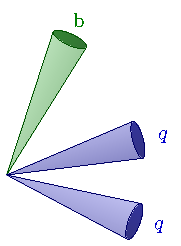
\includegraphics[width=0.28\textwidth]{Feynman/sep.pdf}
    \hfill
    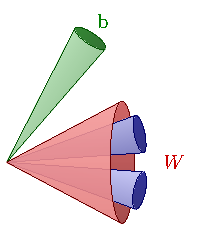
\includegraphics[width=0.28\textwidth]{Feynman/W.pdf}
    \hfill
    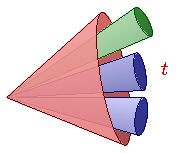
\includegraphics[width=0.28\textwidth]{Feynman/top.pdf}
    \caption{A top quark decay with increasing momentum, showing the transition from three separately resolved jets (left), to a $W$-jet and a $b$-jet (middle), to a single fat jet (right).}
    \label{fig:jet_topologies}
\end{figure}

The number of subjets and the angular separation of these subjets can be used to identify the initiating particle.
One commonly used set of observables to describe jet substructure is its \emph{N-subjettiness}~\cite{Subjet}, denoted by ${\tau_N}$.
N-subjettiness is a measure of how well a jet can be decomposed into $N$ subjets.
For a given $N$ these subjets can be found via some other clustering algorithm, such as the exclusive-$k_t$ algorithm~\cite{ExclusiveKT}, and then the $\tau_N$ observable is defined as,
\begin{equation}
    \tau_N = \frac{1}{\pt R} \sum_{i} \min(\Delta R_{1,i}, \Delta R_{2,i}, \ldots, \Delta R_{N,i}),
\end{equation}
where $k$ runs over the constituents of the jet, and $\Delta R_{i,j}$ is the angular separation between the $i$th constituent and the $j$th subjet.
The discriminating variable for jet tagging is often the ratio of these observables, $\tau_{21} = \sfrac{\tau_2}{\tau_1}$, is commonly used to distinguish vector boson jets from QCD jets, and
$\tau_{32} = \sfrac{\tau_3}{\tau_2}$, is used to identify top quark jets.

Other commonly used observables relate to the jet's energy correlation functions~\cite{ECF} and their ratios.
Analyses at ATLAS make frequent use of the $\Dtwo$ observable~\cite{ATLASD2} to separate 1-prong and 2-prong jets,
\begin{align}
    \Dtwo & = \frac{e_3}{(e_2)^3}, \\
          & = \frac{
        \sum_{1 \leq i < j < k \leq N} z_i z_j z_k \Delta R_{ij} \Delta R_{ik} \Delta R_{jk}
    }{
        (\sum_{1 \leq i < j \leq N} z_i z_j \Delta R_{ij})^3
    },
\end{align}
where $z_i$ is the \pt fraction of the jet carried by the $i$th constituent, and $\Delta R_{ij}$ is the angular separation between the $i$th and $j$th constituents, and $N$ is the number of constituents in the jet.
Additionally, the Energy Flow Polynomials~(EFPs)~\cite{EFP} are a set of basis features which are sensitive to the underlying substructure of different jet types.

\subsection{Heavy-Flavour Tagging}
\label{sec:flavour_tagging}

Heavy-flavour tagging, or simply flavour tagging, is the process of identifying jets that contain the decay products of $b$-quarks ($b$-jets) or  $c$-quaks ($c$-jets).
Jets originating from the decay of $u-$, $d-$, $s-$ quarks and gluons are collectively called light-jets.
Identifying jets from either process is known as $b$-tagging or $c$-tagging, respectively.
In ATLAS, $b$-tagging plays a critical role in many analyses, particularly those measuring properties of the Higgs boson or the top quark.
Nearly all top quarks decay rapidly into a $W$-boson and a $b$-quark, and the dominant decay mode of the Higgs boson is to a pair of $b$-quarks.

Unlike the methods to distinguish large-radius jets, which rely on the jet substructure, the main distinguishing feature used in $b$-tagging is the extended lifetime of hadrons containing $b$-quarks.
As discussed in \Cref{sec:electroweak}, the weak interaction CKM matrix is nearly diagonal, thus favouring transitions within the same generation.
However, the $b$-quark is approximately 40 times lighter than the $t$-quark; it can only decay into lighter generations and is thus CKM suppressed.

The $b$-hadrons are quasi-stable bound states between a $b$-quark and one or two lighter quarks.
They have an average lifetime of around $1.5~\ps$, and if emitted with $\pt=50~\GeV$ would travel around $L_{xy} = 5~\mm$ in the transverse plane before decaying.
This distance can be resolved by the ID vertex fitting algorithms and would result in a vertex with a notable transverse displacement, as shown in \Cref{fig:btagging}.
The presence of a high mass secondary vertex within a jet is the primary feature used in $b$-tagging

\begin{figure}[htb]
    \centering
    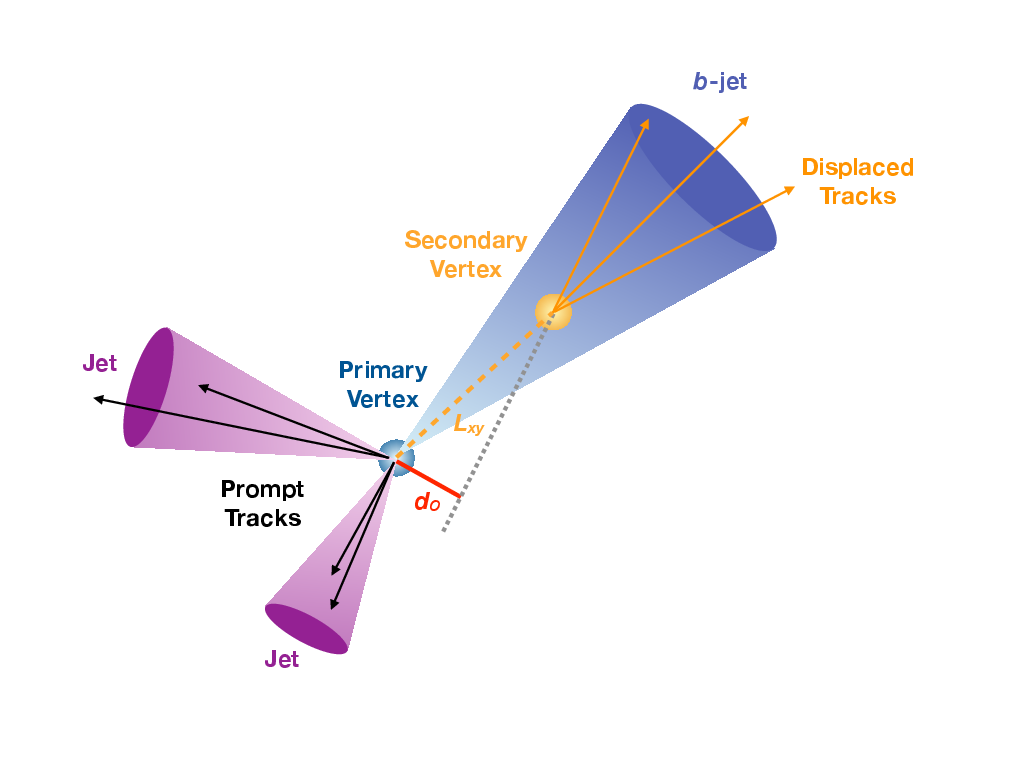
\includegraphics[width=0.75\textwidth]{Figures/cern_atlas/bjet.png}
    \caption{An interaction producing two light-flavour jets and one $b$-jet in the transverse plane. $B$-hadrons have a transverse decay length $L_{xy}$ of a few millimetres, creating displaced tracks and a secondary vertex. The transverse impact parameter (d0) is the closest approach distance of these tracks to the primary vertex, typically large for b-hadrons. Image taken from Ref.~\cite{BJetImage}.}
    \label{fig:btagging}
\end{figure}

Flavour tagging at ATLAS has evolved over many years.
Typically, the tools return the likelihood of a $b$- $c$- or light-jet, given some properties of the associated tracks.
A collection of comparisons between these algorithms used in $b$-tagging is shown in \Cref{fig:btagging_roc}.
Several handcrafted algorithms were designed for flavour tagging before the start of Run 1, such as IPxD~\cite{IPxD}, SV1~\cite{SV1}, and JetFitter~\cite{JetFitter}.
Each tagger used a unique approach to extract different high level features from the jet and associated tracks.
They also yielded different performances depending on the phase space.
It was found that combining the most discriminating features from each in a single neural network resulted in a more versatile tagger known as MV1~\cite{MV1}, which was used at the start of Run 1.
At the start of Run 2, it was replaced by MV2~\cite{MV2}, a boosted decision tree with similar inputs.
In 2017, it was replaced by DL1~\cite{DL1}, a neural network again with much the same approach.
These figures plot the $b$-jet efficiency against light and $c$-jet rejection.

Also introduced at this time was the first tagger based purely on the raw collection of tracks and their parameters, known as RNNIP~\cite{RNNIP}.
This was a recurrent neural network (RNN) that processed all the tracks in the jet sequentially to determine the three class probabilities.
Again, the performance could be improved by combining the outputs of RNNIP with the other IPxD, SV1, JetFitter.
This combination yielded the DL1r tagger~\cite{Run2FTAlgs}.
A second track-based tagger known as DIPS~\cite{DIPS} was developed in 2020.
It used the deep sets architecture~\cite{DeepSets}, and the corresponding combined tagger was labelled DL1d~\cite{AlexThesis}.

The most recent iteration is a departure from the previous approach of combining multiple high level and track based taggers.
In 2022 ATLAS introduced the GN1 tagger~\cite{GN1} which is a graph neural network, \Cref{ch:gnns}, that only uses the track information.
This single network, as shown in \Cref{fig:gn1}, simultaneously performs jet tagging, as well as vertex matching and track classification trained end-to-end.

More details on the GN1 tagger are provided in \Cref{ch:spice}, which also details the development of a new flavour tagging algorithm, GN2, which would supersede it.

\begin{figure}[h]
    \centering
    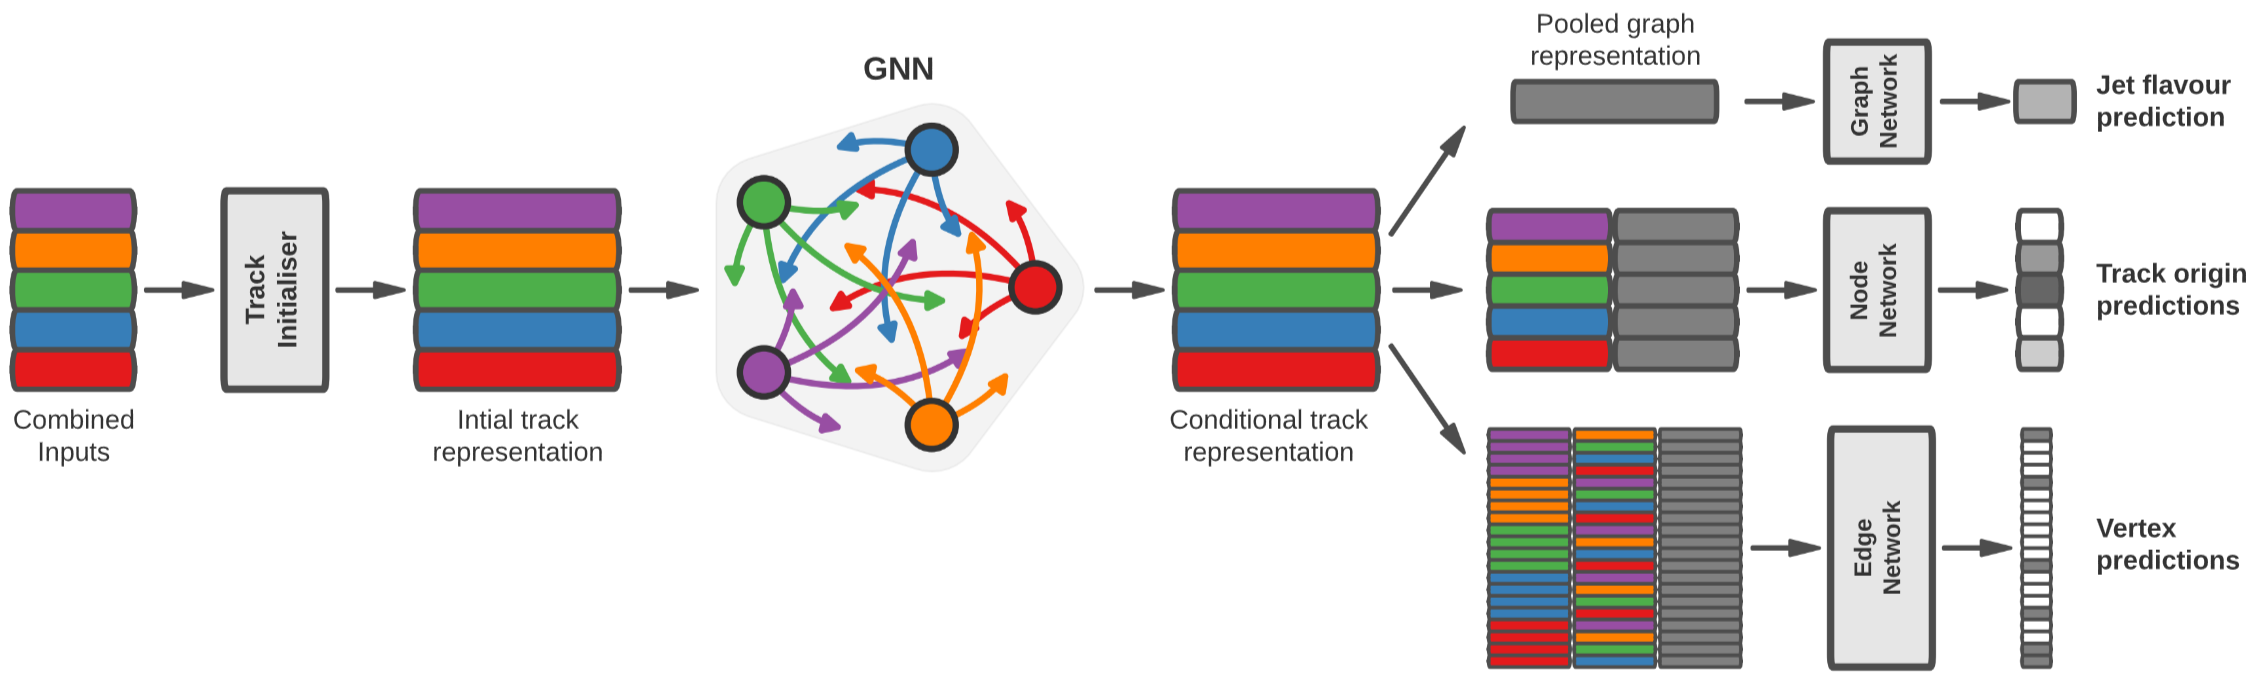
\includegraphics[width=0.99\textwidth]{Figures/cern_atlas/GN1.png}
    \caption{Schematic diagram of the GN1 model from Ref.~\cite{GN1}.}
    \label{fig:gn1}
\end{figure}


\begin{figure}[h]
    \centering
    \begin{subfigure}{0.435\linewidth}
        \centering
        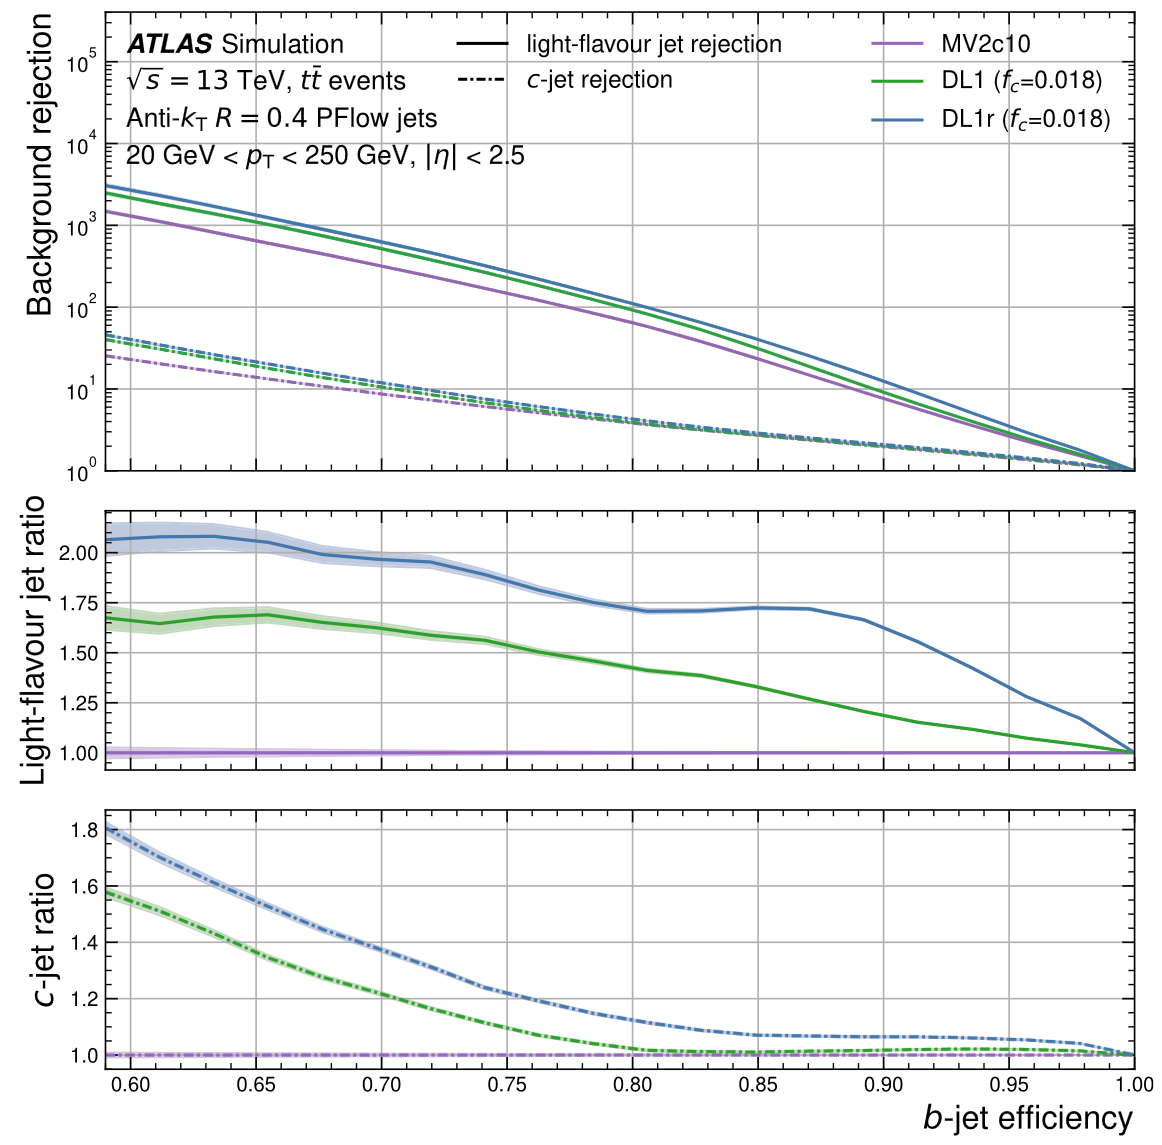
\includegraphics[width=\linewidth]{Figures/cern_atlas/dl1r.png}
        \caption{}
        \label{fig:dl1r}
    \end{subfigure}
    \begin{subfigure}{0.555\linewidth}
        \centering
        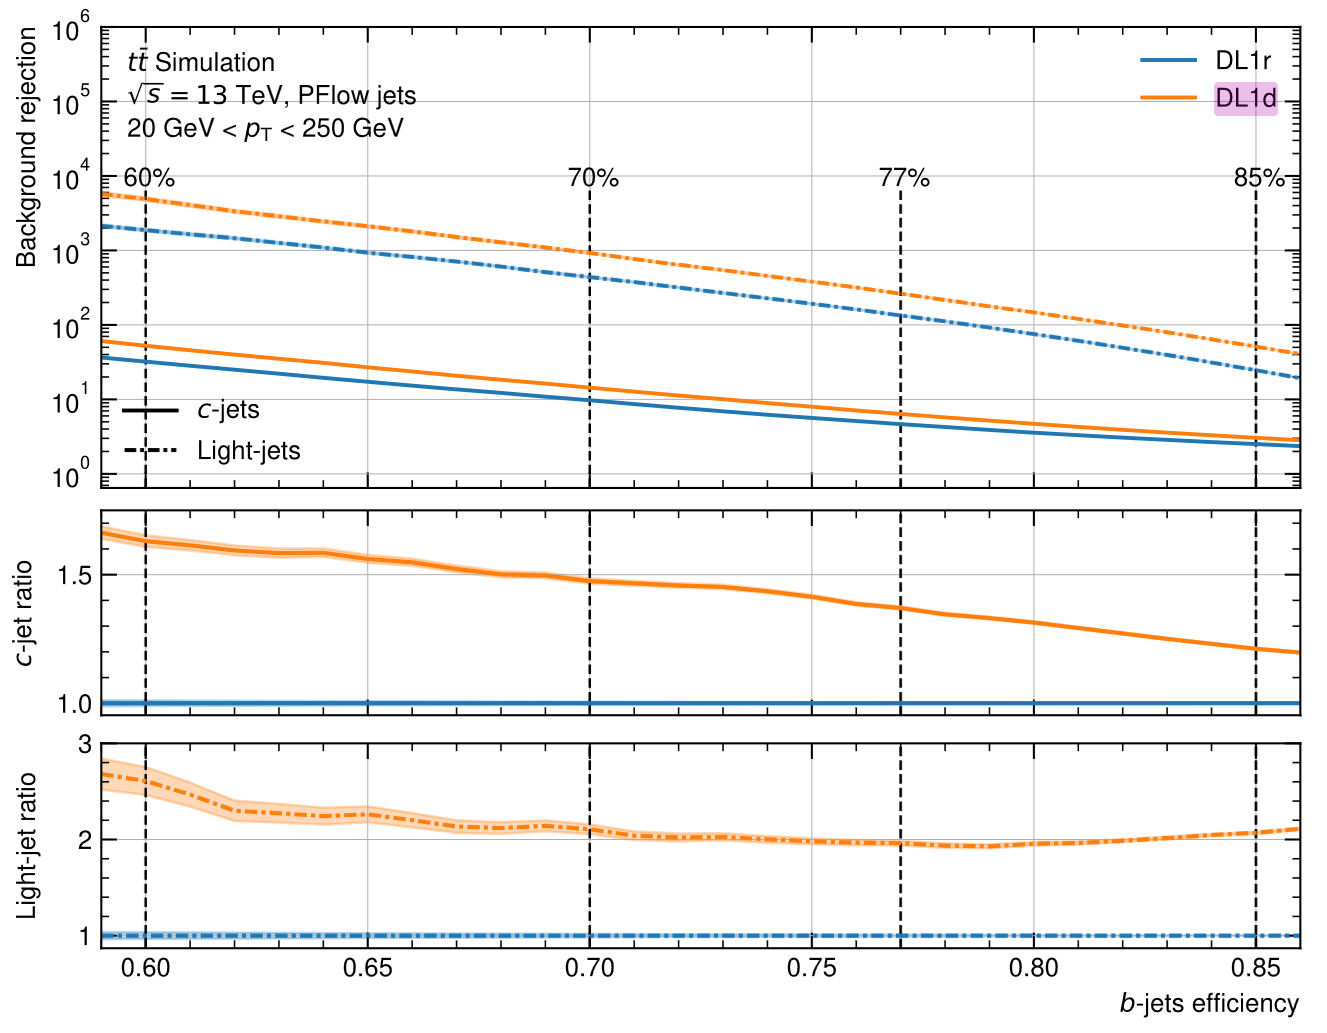
\includegraphics[width=\linewidth]{Figures/cern_atlas/dl1d.png}
        \caption{}
        \label{fig:dl1d}
    \end{subfigure}
    \begin{subfigure}{0.85\linewidth}
        \centering
        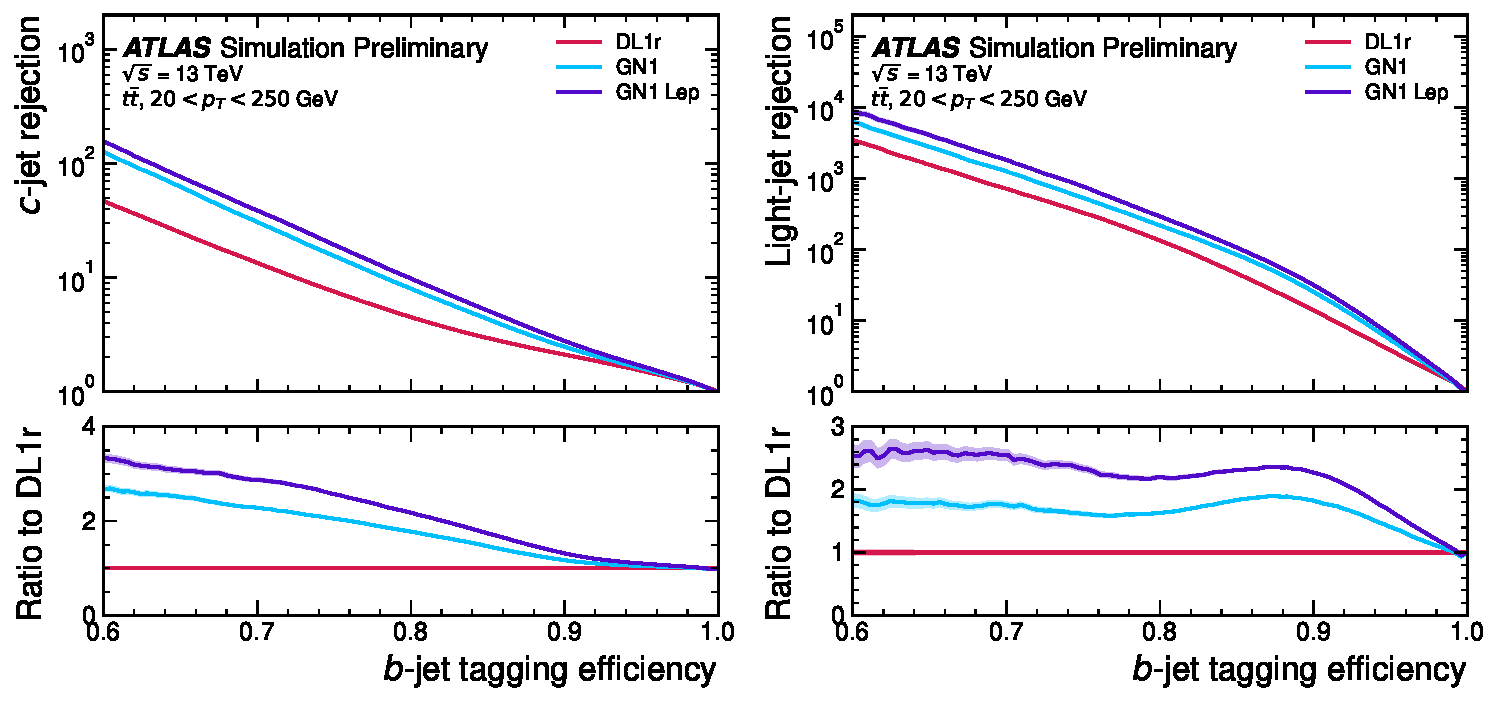
\includegraphics[width=\linewidth]{Figures/cern_atlas/gn1roc.pdf}
        \caption{}
        \label{fig:gn1r}
    \end{subfigure}
    \caption{The rejection factors for light-jets and c-jets as a function of the $b$-tagging efficiency for the different algorithms used by ATLAS over the years as measured on simulated \ttbar datasets. \subref{fig:dl1r} shows the performance of the MV2, DL1, DL1r taggers with the bottom panels showing the performance ratio to MV2. \subref{fig:dl1d} shows the performance of the DL1d and DL1r taggers with the bottom panels showing the performance ratio to DL1r. \subref{fig:gn1r} shows the performance of the GN1 tagger. Images taken from Refs.~\cite{Run2FTAlgs,AlexThesis,GN1} respectively.
    }
    \label{fig:btagging_roc}
\end{figure}

% \chapter{Deep Learning Basics}
\label{ch:deep_learning}

Deep learning has revolutionized the field of collider physics, and the performance gain observed in many algorithms used in the ATLAS experiment has been substantial.
One of the most successful stories has been deep learning based algorithms for flavour tagging, covered in \Cref{sec:flavor_tagging}.
However, despite the enthusiastic integration of ML tools and techniques in HEP, the swift pace of advancements presents a unique challenge.
Researchers often find themselves in a situation where, by the time a newly developed ML tool is implemented and fully integrated into experiments, the technology has already progressed, leading to newer methodologies that render previous tools obsolete.
In addition, experimentalists in HEP favour tools with greater, robustness, and domain adaptation.
The final point is relevant as most models are trained on simulated data.

This chapter provides a brief introduction to deep learning, focusing on the core concepts and techniques that are relevant to the rest of the thesis.

\section{Definition}

Deep learning is the subset of machine learning that focuses on the development and training of artificial neural networks.
These neural networks take the form of a series of composable, parametrized, and differentiable transformations that map input data to output data.
Training or optimization of the networks is done by modifying the parameters of each transformation to minimize some error metric evaluated over a dataset.
The exact form of how the error metric or loss function is calculated differentiates the various types of learning, such as supervised, unsupervised, self-supervised and reinforcement\footnote{There is often overlap between these categories}.

Initially, artificial neural networks were inspired by the structure of the brain, with many layers of interconnected artificial neurons processing information and sending signals to each other.
While individual neurons are simple, the emergent behaviour of the network can be complex.
As the field has evolved, the initial biological inspiration of neural networks has given way to more abstract, mathematical descriptions.
Today, network design is driven by inductive biases, computational efficiency, observations in training dynamics, and (above all) empirical results.
From this more practical perspective, an artificial neural network is long computational graph composed of differentiable operations arranged in layers that transform between collections of real-valued tensors.
The ``depth'' of a deep learning model often refers to the number of layers used in the network.

The primary distinction between deep learning and other parametrized curve fitting methods is simply a matter of scale.
Modern networks now contain billions of parameters, requiring large datasets, specialized hardware, and sophisticated optimization algorithms to train effectively.
As the networks have grown in size and complexity, model interpretability has become a significant challenge and an active area of research.

\section{Supervised Learning}
\label{sec:supervised_learning}

Supervised learning is often introduced first in a pedagogical setting, as it is the simplest and most intuitive form of machine learning. While it is not limited to deep learning, it is introduced here within its context as it is arguably the most common form of training for deep models. Indeed, many other training frameworks, such as reinforcement learning, are reframed as supervised to facilitate training.

In supervised learning, a single data sample is a coupling of two variables $(x, y)$ and is drawn from unknown joint distribution $p_{XY}(X, Y)$.
In this setting, $x$ is the observable information about the sample, and thus the input for a model, and $y$ is some truth label, target, or desired output for a model.
The goal of supervised learning is to produce a discriminative model which approximates the mapping from inputs to outputs, $f: X \rightarrow Y$.
Discriminative models can also be probabilistic, where they model the conditional probability distribution of the target given an observation $f(x, \hat y) \approx p_Y(Y=\hat y|X=x)$.
Probabilistic models which permit sampling from this distribution can also be considered generative models, which are covered in \Cref{ch:generative_models}.

Fitting or training a supervised learning model typically requires a training set $\mathcal{D}$ containing of $N$ observations and their paired targets $\mathcal{D} = \{(x_i, y_i)\}_{i=1}^N$.
These samples are usually assumed to be independent and identically distributed (i.i.d.) from the joint\footnote{Non i.i.d. data can sometimes be used by incorporating the appropriate weights during training}.
A supervised learning algorithm $f$, probabilistic or not, is selected out of some hypothesis space $\mathcal{H}$ to minimize some measure of empirical risk $\mathcal{R}$ over the training set.
\begin{equation}
    f = \argmin_{f \in \mathcal{H}} \frac{1}{N} \sum_{i=1}^N \mathcal{R}(f, (x_i, y_i)).
\end{equation}

For now, no assumptions are made about the structure of the input or output samples, except that they can be represented as tensors, or collections of tensors, of real numbers.
Common types of supervised algorithms $f$ including support vector machines, decision trees, and of course neural networks.
For a neural network $f_{\theta}$, the hypothesis space $\mathcal{H}$ is the set of all possible network architectures and network parameter values $\theta$.

\section{Network Design}

A single network layer is any function parametrized by a set of variables $\theta$ that can takes in a set of input tensors and returns a set of output tensors (both could be sets of size one).
There are very few limits on what exactly this function can be, but there are some core design principles ML engineers have to rely on when designing a network to solve a specific task.
These principles are called inductive biases~\cite{InductiveBiases1, InductiveBiases2}, and they are the assumptions made to allow a learning algorithm to favour one solution over another.
Inductive biases do not have to be explicitly defined.
For example, fitting a linear regression model explicitly assumes that the relationship between the input and output is linear, but doing so using mean squared error implicitly assumes that the relationship is corrupted by Gaussian noise with constant variance.

There exists a vast array of possible network layers, each with their own inductive biases, some as simple as affine transformations, others as complex and composite as multi-headed attention layers~\cite{Attention}.
Much of the art of deep learning is the design and composition of these layers to create a network that can solve a specific task.
One rough philosophy is that individual layers should be simple and easy to implement.
This is because neural networks are compositional, and it is the application of many of these highly parametrized layers in series that gives the network its expressive power.

As it is in physics, exploiting symmetries of the data structure is a good core principle to follow and many layers are designed with equivariance or invariance in mind.
Convolutional layers~\cite{DeepLearning} are well suited for image or otherwise grid-like data with localized features as they are somewhat equivariant to translations.
Message passing networks~\cite{NeuralMessagePassing} work well for graph data as they are equivariant to the permutation of the nodes.
GATr~\cite{GeometricAlgebraTransformer} layers are designed under the principles of Clifford algebra to operate on geometric data and are equivariant to rotations and translations.
LorentzNet~\cite{LorentzNet} operates on particle physics data and is designed to be equivariant to boosts in reference frame.
There exist many more examples of layers designed with specific data and symmetries in mind.

For deep learning, examples of inductive biases include the choice of loss function, regularization, the optimization algorithm, and even the model architecture itself.
Weight decay can be seen as an inductive bias towards simpler models, as it prioritizes solutions with small parameters.
Ideal inductive biases should improve the performance of the model primarily by aiding the optimization process.
However, too restrictive biases can limit model performance by excluding valid solutions.
Inductive biases can also be understood in terms of the bias-variance trade-off, where flexibility is traded for generalization.

\subsection{The Multi-Layer Perceptron}

The Multi-Layer Perceptron (MLP) is arguably the simplest form of a deep neural network.
It is also referred to as a dense network, fully connected network, or sometimes confusingly as a feed-forward neural network (FFN)\footnote{A term which can be used to describe any neural network without loops in the computational graph.}.
In an MLP, there is a single input and single output both of which are rank-1 tensors, but can have differing numbers of features.
A minimal working example of an MLP is a series of affine transformations\footnote{Often called a linear layer, but the operation almost always includes a bias term.}, each parametrized by a weight matrix $\W$ and bias vector $\bias$, followed by a non-linear activation function $\sigma$.
The depth of the MLP is the number of intermediate representations in the computational graph between the input and output.
A minimal MLP with two hidden layers can be written as
\begin{align}
    \ba_0 & = \x,                                        \\
    \ba_1 & = \sigma_0(\W_0 \ba_0 + \bias_0),            \\
    \ba_2 & = \sigma_1(\W_1 \ba_1 + \bias_1),            \\
    \ba_3 & = \sigma_2(\W_2 \ba_2 + \bias_2) = \hat{\y},
\end{align}
where $\x$ is the input, $\hat{\y}$ is the output, and $\ba_i$ are the intermediate representations (or activations) of the network.
The parameters of this network are is the full set of weights and biases from each layer, $\theta = \{W_0, \bias_0, W_1, \bias_1, W_2, \bias_2\}$.
Each layer can arbitrarily resize the input tensor based on the shapes of the weight matrix and bias vector.

Activation functions exist to introduce non-linearities in the computational graph and are applied elementwise to the tensors.
As the composition of affine transformations is itself an affine transformation, without activation functions, the entire MLP could be reparametrized as a single affine transformation, no matter its depth, greatly hindering its expressive power.
With these induced non-linearities, MLPs can approximate any continuous function between real valued tensors~\cite{ApproximationSuperpositionsSigmoidal, ApproximatingContinuousFunctions, UniversalApproximationDeep}, given enough hidden units and the right activation functions.

The activation function in the output layer is typically chosen to match the expected range of the target variable.
Historically, the sigmoid function was used as the primary activation in the hidden layers, due to its analogy with biological activation.
However, it can be shown that even the simplest function that breaks linearity is sufficient, and the ReLU~\cite{ReLU} function $\text{ReLU}(x) = \max(0, x)$ has become the popular choice for hidden layers in modern networks.
Other common choices for hidden layer activations are shown in \Cref{fig:activations}.

\begin{figure}
    \centering
    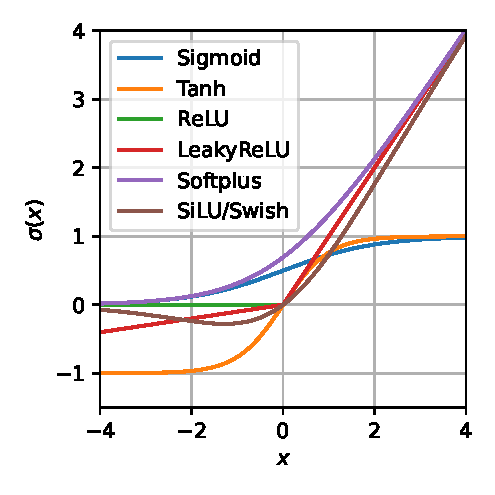
\includegraphics[width=0.4\textwidth]{Figures/deep_learning/activations.pdf}
    \caption{Common activation functions used in deep learning.}
    \label{fig:activations}
\end{figure}

\section{Training with Gradient Descent}

Once a network has been designed, it is typically initialized with random parameter values $\theta$.
Training or fitting a deep neural network is an optimization problem where the best parameters $\theta^*$ are those that minimize the risk, here described as a loss $\mathcal{L}$, over the training set $\mathcal{D}$.
\begin{equation}
    \theta^* = \argmin_{\theta} \frac{1}{N} \sum_{i=1}^N \mathcal{L}(\theta, x_i).
\end{equation}
For generalization, $x_i \in \mathcal{D}$ may also include the target if present.
Due to the size of the parameter space and the non-linearity of the model, the $\theta^*$ cannot be found analytically.
The most common method for training deep neural networks is mini-batch stochastic gradient descent (SGD)~\cite{Perceptron} or one of its many variants.
SGD is an iterative optimization algorithm that attempts to minimize the loss over a dataset by adjusting the parameters of the model in the direction of the negative gradient of the loss calculated over a random subset of the data.
An outline of the basic training algorithm is shown in \Cref{alg:gradient_descent}.
Here $\mathcal{L}(\theta, b)$ is the average loss over a mini-batch of size $B$,
\begin{equation}
    \mathcal{L}(\theta, b) = \frac{1}{B} \sum_{i=1}^B \mathcal{L}(\theta, x_i).
\end{equation}
Both the $B$ and the $\eta$ are hyperparameters of the training algorithm.

\begin{algorithm}
    \caption{Basic training pseudocode for minibatch stochastic gradient descent.}
    \label{alg:gradient_descent}
    \begin{algorithmic}[1]
        \State \textbf{Input:} Training set $\mathcal{D}$, batch size $B$, learning rate $\eta$, stopping criterion
        \State Initialize parameters $\theta$
        \Repeat \Comment{Each loop is an \textit{epoch}}
        \State Shuffle the dataset $\mathcal{D}$
        \State Partition $\mathcal{D}$ into batches of size $B$
        \For{each batch $b$ in $\mathcal{D}$}
        \State Calculate the loss $\mathcal{L}_b(\theta)$ for the batch $b$
        \State Compute the gradient $\nabla_\theta \mathcal{L}(\theta, b)$
        \State Update parameters: $\theta \gets \theta - \eta \nabla_\theta \mathcal{L}(\theta, b)$
        \EndFor
        \Until{stopping criterion is met}
    \end{algorithmic}
\end{algorithm}

Once the entire training set has been processed, this is considered one epoch.
Training continues until some stopping criterion is met, such as a saturation of the loss.
Typically, models are trained for many epochs and the training set is shuffled between each epoch to prevent correlated updates which may hinder convergence.
Ideally we would have $B=N$, this is called batch gradient descent, but this is often infeasible due to memory constraints.
So instead we use a noisy estimate of the gradient, by using a subset of the training set and true SGD uses $B=1$.

The learning rate $\eta$ is a crucial hyperparameter of the training algorithm, however it is common to modify it during training.
Many large networks require a warm-up phase~\cite{SGDRStochasticGradient} where the learning rate is slowly increased from zero to its maximal value.
Without this step, large models like transformers are prone to diverging early in training.
The learning rate is also typically decayed towards the end of training helping the network converge to a local minimum, avoiding oscillation, and improving the learning of complex patterns~\cite{HowDoesLearning}.
Sometimes these phases are repeated, cycling the learning rate up and down again and again~\cite{CyclicalLearningRates}, and sometimes they are performed only once~\cite{SuperConvergenceVeryFast}, ending the training after the first cycle.

There exist many extensions to this basic algorithm that attempt to improve robustness and convergence.
One common method is the accumulation of a moving average of the gradients, analogous to momentum in physics~\cite{Momentum}.
This assists in traversing regions of the parameter space where curvature is higher in one direction than another.
Another common method is the use of adaptive learning rates, where the per parameter learning rate is adjusted based on the fluctuations in the gradient~\cite{Adagrad, RMSProp}.
\Cref{alg:adam} shows the update rule for one of the most common variants, the Adam optimizer~\cite{Adam}, which combines both momentum and adaptive learning rates.
It introduces two hyperparameters $\beta_1$ and $\beta_2$ which control the exponential decay rates of the moving averages.

\begin{algorithm}
    \caption{The Adam optimizer, where $\mathcal{L}(\theta, b)$ is the loss calculated over a mini-batch, $\eta$, $\beta_1$, $\beta_2$ are hyperparameters, $t$ is the current iteration and $\epsilon$ is a small constant to prevent division by zero.}
    \label{alg:adam}
    \begin{algorithmic}[1]
        \State $\mathbf{m} \gets 0$ \Comment{Initialize first moment vector}
        \State $\mathbf{s} \gets 0$ \Comment{Initialize second moment vector}
        \For{each mini-batch $b$}
        \State $\mathbf{g} \gets \nabla_\theta \mathcal{L}(\theta, b)$ \Comment{Compute gradients}
        \State $\mathbf{m} \gets \beta_1 \mathbf{m} + (1 - \beta_1) \mathbf{g}$ \Comment{Update biased first moment estimate}
        \State $\mathbf{s} \gets \beta_2 \mathbf{s} + (1 - \beta_2) \mathbf{g} \otimes \mathbf{g}$ \Comment{Update biased second moment estimate}
        \State $\hat{\mathbf{m}} \gets \frac{\mathbf{m}}{1 - \beta_1^t}$ \Comment{Correct bias in first moment}
        \State $\hat{\mathbf{s}} \gets \frac{\mathbf{s}}{1 - \beta_2^t}$ \Comment{Correct bias in second moment}
        \State $\theta \gets \theta - \eta \frac{\hat{\mathbf{m}}}{\sqrt{\hat{\mathbf{s}} + \epsilon}}$ \Comment{Update parameters}
        \EndFor
    \end{algorithmic}
\end{algorithm}

\subsection{Normalization}

Training via gradient descent requires the gradient with respect to every parameter in the model.
This leads to a balancing problem with the vanishing and exploding gradient problems manifesting as the gradients become too small or too large to be useful for training.
This is especially problematic in deep networks, where the gradients must be propagated through many layers, requiring the repeated application of the chain rule.
As the scale of the gradients are linked to the scale of the activations in each layer, it is good practice to ensure the activations remain within a reasonable range during training.
It is common to target activations with a mean of zero and unit variance through the inclusion of normalization layers.

In addition to stabilizing gradients, normalization layers assist in the expressivity of the networks.
Most activation non-linearities occur near zero, \Cref{fig:activations}.
Oversaturating these functions with large positive or negative values ensure that the layer either becomes linear or constant, depending on the function.
In both cases, the layer can no longer approximate non-linear transformations.

Normalization starts with the input data itself, which can be seen as a preprocessing step or as the first layer of the network.
This is typically performed using the statistics of the training set.
Variables with long tails are also transformed to have a more Gaussian distribution.
This can be done by taking the logarithm of variables with large dynamic ranges, or by using more advanced techniques like a quantile transformation.
Within the network itself, normalization layers $L_{\text{norm}}$ are interleaved between others.
Methods such as batch normalization (BatchNorm)~\cite{BatchNorm} or layer normalization (LayerNorm)~\cite{LayerNorm} are widely used and both have been shown to be greatly effective, with the latter seen as essential for transformer neural networks~\cite{Attention}.

Another feature used to stabilize training is the manual clipping of the gradients before applying the parameter update.
This can be done based on some maximal value, but is more commonly done by scaling the gradient such that their combined norm does not exceed some threshold~\cite{WhyGradientClipping}.

\subsection{Residual Connections}

Residual connections are another simple and effective technique for training deep networks.
Here the learnable transformation of the layer is added to the input, rather than replacing it,
\begin{equation}
    \ba_{i+1} = \ba_i + l(\ba_i),
\end{equation}
where $l$ is the transformation of the layer.
A single operation of this form is called a residual block.
Residual connections have been shown to improve the training of very deep networks, as they allow the gradient to flow directly through the network, bypassing the squashing or exploding effects of the intermediate layers.
Residual connections are a key component of almost all modern architectures from convolutional neural networks~\cite{ResNet} to transformers~\cite{Attention}.
The residual connection is usually additive, but other operations exist, for example UNets~\cite{Unet} use concatenation.
If the input and output of the layer have different dimensions, the residual path can be adjusted by a minimal transformation, in a convolutional network this is typically a $1 \times 1$ convolution.

The addition of two signal paths means that $a_{i+1}$ will have a larger variance than $a_i$.
This can cause a deeper network to become unstable, especially in the early stages of training.
One method to circumvent this is the inclusion of a normalization layer after the residual block, as was done in the original transformer architecture~\cite{Attention}, which is referred to as post-normalization.
However, this was shown to be detrimental in very deep networks and recent methods use pre-normalization (PreNorm)~\cite{PreLN}, where the input to the learnable layer is normalized.
With a PreNorm residual block one can prevent an exploding variance problem by scaling the residual path by a small coefficient, such as $\frac{1}{\sqrt{2}}$~\cite{StyleGAN2}.
Recent methods initialize this coefficient to zero, such that the block behaves like an identity function, but allow it to be learned during training~\cite{ReZero, SkipInit, Fixup}.
This was extended to the LayerScale method~\cite{GoingDeeper}, where a fully learnable tensor $\mathbf{L}_\text{scale}$ matching the output shape of the layer is used to scale the residual path.
Initialized to zero, the network will learn the optimal scaling during training.

A PreNorm residual block with LayerScale follows,
\begin{equation}
    \ba_{i+1} = \ba_i + \mathbf{L}_\text{scale} \otimes f( L_{\text{norm}}(\ba_i) ),
\end{equation}
where $\otimes$ is elementwise multiplication.
Such a layer structure can be applied in many types of networks, from MLPs~\cite{InvertedBottleneck} to transformers~\cite{GoingDeeper}.

\section{Generalization}

Generalization in the context of ML refers to the ability of a model to perform well on new, unseen data.
This is in most cases the primary goal of training such a model.
As neural networks are highly flexible, it is possible that they can ``memorize'' the training set, achieving a very low loss during training, but not matching that performance on new data.
This phenomenon is called overfitting, and it is a common problem in deep learning.

Overfitting may be detected during training through cross-validation.
The most simple case of this is to split the available data into a training set and a validation set.
Gradient descent is performed on the training set, but the loss is also calculated over the validation set at regular intervals.
The difference in performance between the training and validation set is a good indicator of overfitting.
Often the model chosen for future applications is the one that performs best on the validation set.

There are many methods to combat or reduce overfitting.
Regularization methods are techniques that affect the training process.
Weight decay includes extra terms in the loss function that impose a penalty based on the magnitude of the parameters in the network, pushing it towards simpler solutions.
Dropout~\cite{Dropout} is a technique where a random subset of the activations in the network are set to zero during training, effectively training an ensemble of models.
Alternatively, dropout simply injects noise into the network, which can help prevent overfitting.
Drop-path and stochastic depth~\cite{DeepNetworksStochastic} is an extension of dropout where entire residual layers are removed from the network during training.
Data augmentation can also help by artificially expanding the training dataset.
Confusingly, increasing the size of the network can also help prevent overfitting.
This is known as the double descent phenomenon~\cite{UnderstandingDoubleDescent}, whereas the effective model capacity grows, more solutions become accessible, and the model becomes a self ensemble.

Domain shift is a problem which is similar to overfitting, but occurs when the underlying distribution of the training and test datasets differ.
This is a significant issue in HEP, where models are trained on simulated samples, in order to have access to ground truth labels, but must be applied to real data.
Domain adaptation~\cite{UnsupervisedDomainAdaptation} and adversarial training~\cite{EnhancingGeneralizationHigh} are methods to address this.

Finally, unwanted biases in the training set can lead to skewed predictions.
The distribution of the target variable in supervised settings acts as a prior for the model, and if this distribution is not representative of the population, the model will make biased predictions.
Reweighting or resampling the training set can help mitigate this.

% \chapter{Graph Neural Networks}
\label{ch:gnns}

The philosophy behind graph neural networks (GNNs) is rooted in the idea that nature is best understood when broken down into compositional elements.
By understanding these elements and the rules governing their interactions, we can gain insights into the system as a whole.
This reductionist approach is used in many areas of science, and indeed is the basis for all of particle physics.

Graphs serve as a prime example of explicitly structured data, encompassing entities and their pairwise relationships. GNNs are a type of deep learning model designed to handle this structure, allowing information to flow through the network in a manner that mirrors the graph's organization.

This chapter explores the foundational principles of GNNs, how they operate, and their limitations.
It also delves into the most successful GNN variant to date, the transformer model, which is utilized extensively in the subsequent chapters of this thesis.
This chapter follows the notation and formalism of~\textcite{RelationalInductiveBiases}.

\section{Learning Relations}

Relational reasoning~\cite{SimpleNeuralNetwork} is the development of rules that describe how the properties of entities modify the relations between them, and how in turn the relations modify the properties of the entities.
GNNs employ relational reasoning to complete tasks by directly manipulating the rules, entities, and relations of a system.

An example of successful relational reasoning being used in deep learning outside GNNs is in image processing tasks.
An image is typically represented as a rank-3 tensor using the pixel values as the tensor elements.
This tensor of has shape $(H, W, C)$, where $H$ and $W$ describe the image resolution, and $C$ is the number color channels.
If one wanted to process this tensor with an MLP, it must first be flattened to a have of shape $H \times W \times C$.
Within each affine layer every element of the input tensor is connected to every element of the output tensor.
While this leads to a flexible model, it also destroys the spatial structure of the image and no reusable relationships or rules are used.

Alternatively, we could use a network composed of learnable convolutional kernels.
These kernels scan over the input tensor, computing the weighted sum of the elements within the kernel window.
This introduces two key relational inductive biases: locality and translation invariance.
Locality refers to the assumption that the relationship between two elements is stronger if they are close together in the input space.
Translation invariance refers to the assumption that the relationship between two elements is the same regardless of their absolute position in the input space.
Locality is enforced by using a kernel width of limited size and translation invariance is enforced by reusing the same kernel across the whole image.
Each convolutional kernel defines rule for how elements within the structure of the input tensor are related.

This is an example of geometric deep learning, also called a relational inductive bias, whereby the known structure of the data is embedded into the architecture of the model itself, rather than being learned directly from the data.
This reduces the number of parameters required in the model, allowing for more statistically efficient learning.

\section{Defining a Graph}

A graph $\mathcal{G}$ is a data structure that consists of a set of $N$ attributed nodes $\mathcal{N} = \{\x_i\}_{i=1}^{N}$ interconnected by a set of $N^e$ attributed edges $\mathcal{E} = \{(\x_k, r_k, s_k)\}_{k=1}^{N^e}$.
Here $\edge_k$ are the edge attributes, and $s_k$ and $r_k$ are the indices of the sender and receiver nodes in $\mathcal{N}$ respectively.
It is also useful in many contexts to define a global attribute $\u$ which describes the graph as a whole.
A singular-graph can be represented as a tuple $\mathcal{G} = (\mathcal{N}, \mathcal{E}, \u)$.
The structure of the graph is only defined by the interconnections between the nodes, the actual ordering of the nodes in the set is arbitrary.
Therefore, any operation on the graph should not depend on this order.
Note that the adjacency matrix of the graph is not explicitly defined, but can be inferred from the elements of $\mathcal{E}$.

This description of a graph is very general and each of the terms $\mathcal{N}$, $\mathcal{E}$, and $\u$ are optionally included.
We could allow multiple sets of edges to exist between nodes $\{\mathcal{E}^1, \mathcal{E}^2, \ldots\}$, defining a multi-graph.
Each of the edge $\x_i$, node $\edge_{k}$, and global $\u$ attributes can also be encoded as any type of representation, even graphs themselves.
In most use cases dealt with in this thesis, each of $\x_i$, $\edge_k$, and $\u$ are real valued tensors.
It is also common for all the nodes to share the same dimensionality, and the same for the edges, imposing an equivalence between the elements of the set.
This it simplifies the design of the model as it allows operations on the individual elements to be parameterized with standard building blocks, such as affine layers, MLPs, and CNNs.

Representing a graph in code requires tuple or dictionary of real valued tensors $(\x, \edge, \u)$.
Here, $\x \in \mathbb{R}^{N \times d}$, $\edge \in \mathbb{R}^{N \times N \times d_e}$, and $\u \in \mathbb{R}^{1 \times d_u}$, where $d$, $d_e$, and $d_u$ are the dimensionality of the node, edge, and global features respectively.
The edge matrix is typically ordered such that $\edge_{ij}$ is the edge from node $i$ to node $j$.
To represent the existence or absence of an edge between two nodes, a binary adjacency matrix $\mathbf{A} \in \{0, 1\}^{N \times N}$ can be used where $\sum{\mathbf{A}} = N^e$.
Alternatively, one could use a sparse tensor representation, which is more memory efficient but can complicate the implementation of the model.

Almost all GNNs operate by facilitating message passing between the nodes of the graph.
In this framework each node sends messages to their neighbours.
These messages are then aggregated and used to update the node's attributes.
Exact details of how this is done can vary between models, but the core idea is the same.

\begin{figure}
    \centering
    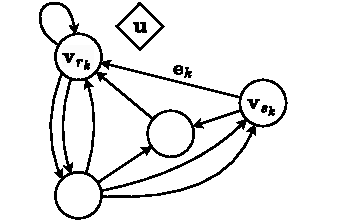
\includegraphics[width=0.5\textwidth]{Figures/graph_networks/graphs.pdf}
    \caption{A directed multi-graph with node, edges a global attribute $\u$. Highlighted is the edge $\edge_{k}$ which connects the sender node $s_k$ to the receiver node $r_k$.}
    \label{fig:graph}
\end{figure}

\section{Graph Type Data}
\label{sec:graph_data}

Graph or set representation is fairly ubiquitous in the real world as it may be used for anything that can be broken down into discrete elements.
For instance, a collection of particles captured by a detector can be expressed as sets, where the stable particles are the nodes and their attributes are the particle kinematics.
This is a natural representation because, for a single collision event, there is no inherent ordering to the outgoing particles.
This is natural representation as for a single collision event, there is no inherent ordering to the outgoing particles.
Some other examples are shown in \Cref{fig:graph_examples}.
Particle interactions and decay chains, such as the all-hadronic $ttH$ production process shown in \Cref{fig:feynman}, can be represented as a graph.
In this situation, it might be more natural to represent the particles in the Feynman diagram as edges rather than the nodes.
Chemical compounds can also be easily represented as graphs, where the atoms are the nodes and the chemical bonds between them are the edges.

Even data which is not inherently graph-like can be broken down into constituent parts and interconnected to form a graph.
Text can be \textit{tokenized} by treating words or subwords as nodes~\cite{Attention} and images may be segmented into patches \Cref{fig:dog}.
Though graphs typically have no natural ordering, text and image patches would not make sense if shuffled, thus order has to be imposed by the model.
This can be done by including the position of the node in its attributes or limiting the edges to only connect the nodes in a predetermined order.
This is covered in more detail in \Cref{sec:edge_biases_sequences}.

In analysing graph data within real-world contexts, there exists three primary types of predictive tasks: graph-level, node-level, and edge-level predictions.
For graph-level tasks, the aim is to predict an attribute or property that encompasses the entire system as a whole.
An example of this in the context of computer vision would be the classification of the entire image.
Node-level tasks predict the properties associated with each individual node.
Finally, there are edge-level tasks which predict properties or even the existence of edges between the nodes.

\begin{figure}
    \centering
    \begin{subfigure}[b]{0.45\textwidth}
        \centering
        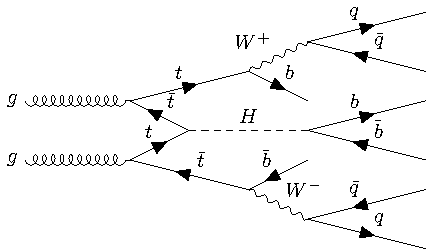
\includegraphics[width=\textwidth]{Feynman/tth.pdf}
        \caption{Particle interactions}
        \label{fig:feynman}
    \end{subfigure}
    \begin{subfigure}[b]{0.45\textwidth}
        \centering
        \includegraphics[width=\textwidth]{Figures/graph_networks/RifampiciN_Structure.pdf}
        \caption{Chemical compounds}
        \label{fig:chemical}
    \end{subfigure}
    \begin{subfigure}[b]{0.45\textwidth}
        \centering
        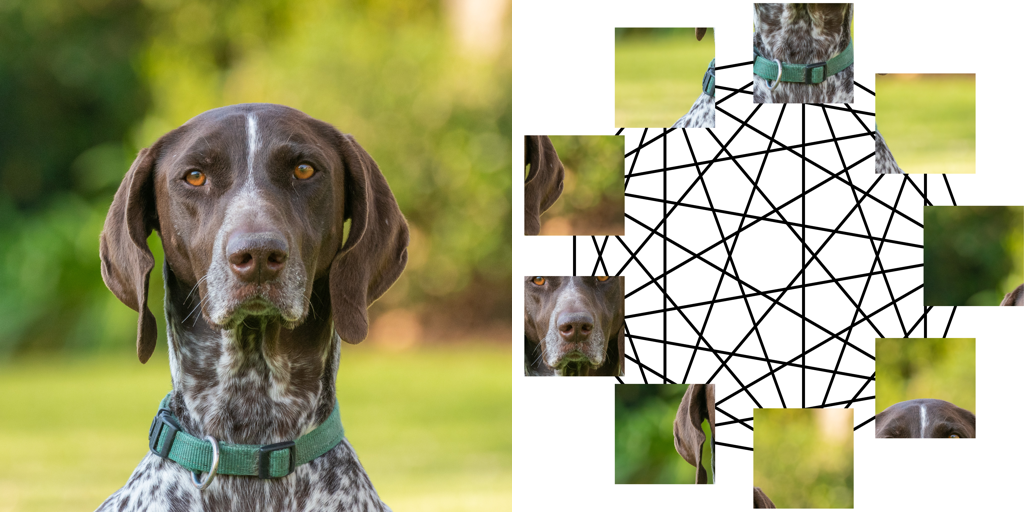
\includegraphics[width=\textwidth]{Figures/graph_networks/patched_image.png}
        \caption{Images (patched)}
        \label{fig:dog}
    \end{subfigure}
    \begin{subfigure}[b]{0.45\textwidth}
        \centering
        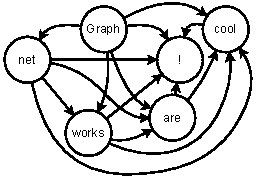
\includegraphics[width=0.8\textwidth]{Figures/graph_networks/text.pdf}
        \caption{Language (tokenized)}
        \label{fig:text}
    \end{subfigure}
    \caption{Examples of data that can be represented as graphs.}
    \label{fig:graph_examples}
\end{figure}

\subsection{Interconnectivity}

When constructing a graph representation it is crucial to consider its interconnectivity; which pairs of nodes have edges between them.
GNNs propagate information along edges, so the structure of the graph can have a significant impact on the model's performance.
Interconnectivity is closely tied to two key issues in GNNs: over-squashing~\cite{OverSquashing} and the over-smoothing~\cite{OverSmoothing}.

The inductive bias of locality can be imposed in a graph by only connecting nodes close to each other in some metric space.
However, limiting the connections of each node to its local neighbourhood can also mean that long term dependencies may get lost.
This is because multiple rounds of message passing are required to propagate information between distant nodes as shown in \Cref{fig:neighbours}.
With each round, exponentially more neighbouring nodes need to project information into a fixed-size vectors leading to an over-squashing of information.
It is exacerbated by bottlenecks in the graph structure as shown in \Cref{fig:bottleneck}, where the information between nodes $\x_i$ and $\x_j$ must pass along a single edge which must also carry information from their respective neighbourhoods.

There are many proposed solutions to the over-squashing problem.
The inclusion of global features in the graph may help model long range dependencies, however the size of the global tensor would need to scale with the cardinality of the set.
Another solution is to simply increase the number of edges in the graph, allowing for more direct paths between nodes.
This is known as graph rewiring and can be focussed around bottlenecks in the graph, identified by regions of low Forman curvature~\cite{UnderstandingOversquashingBottlenecks}.

There are however downsides to graph rewiring.
First, it means loosening the locality inductive bias.
The extreme case of this is a fully connected graph, where edges exist between all pairs of nodes in both directions and locality is completely lost.
Secondly, is that it exacerbates the other issue with GNNs, over-smoothing.
This refers to the phenomenon where all node features across the graph converge towards the same constant value as the number of message passing steps increases.
This one of the reasons that the depth of most GNNs is notably shallower than other deep learning models, as with every round of message passing each node aggregates information from its neighbours, diluting the original information.
There are many proposed solutions to this issue, such as residual connections~\cite{DeepGCNs}, normalization layers~\cite{PairNorm}, and regularization~\cite{DirichletEnergyConstrained}.
Finally, there is a computational cost to increasing the number of edges in the graph.
Many models are looking to find way to minimize the interconnectivity while preserving model quality~\cite{GeneratingLongSequences}.

\subsubsection{When is an Inductive Bias Holding You Back?}

As previously mentioned, one of the key inductive biases leading to the success of CNNs is the locality of the convolutional kernel.
However, the state-of-the-art models in computer vision are GNNs operating on fully connected graphs of image patches~\cite{VisionTransformer}, demonstrating that locality in images is not always useful.
This makes intuitive sense, as the content of an image is not always localized; objects can be spread out across multiple patches, and they may be obscured, only visible in physically separated regions of the image.

This extends to the example of the chemical compound in \Cref{fig:chemical}.
In this model the edges are defined by the chemical bonds between the atoms.
However, long range dependencies do exist in chemistry.
The function of one part of a protein may be altered by the presence of a ligand on the other side of the molecule.
Constraining the message passing graph to match the physical graph may limit the model from learning these relationships.

The GNNs that work well in these cases are equipped with all the tools needed to combat over-smoothing mentioned in the previous section, as well as the attention mechanism~\cite{Attention}.
Attention refers the learnable process of weighting the incoming messages before aggregation.
It allows the GNN to ``pay more attention'' to specific connections within the graph.

This raises the point that if we have enough data and a large enough model, enforcing what relationships are important may not be necessary, and it is better to let the model learn these rules itself.
It also raises whether the message passing graph and the input data graph should be tied together at all.
Models such as the perceiver~\cite{Perceiver} project input information onto a completely different latent graph for message passing and recent work for GNNs in computer vision has shown that they require extra, fully learnable nodes not tied to any image patch~\cite{VisionTransformersNeed}.

\begin{figure}
    \centering
    \begin{subfigure}[b]{0.3\textwidth}
        \centering
        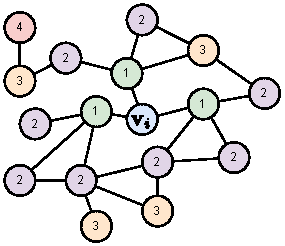
\includegraphics[width=\textwidth]{Figures/graph_networks/neighbours.pdf}
        \caption{}
        \label{fig:neighbours}
    \end{subfigure}
    \begin{subfigure}[b]{0.3\textwidth}
        \centering
        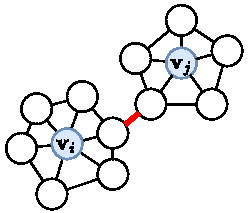
\includegraphics[width=\textwidth]{Figures/graph_networks/bottleneck.pdf}
        \caption{}
        \label{fig:bottleneck}
    \end{subfigure}
    \caption{\subref{fig:neighbours} The locality of information flow in a graph. On each node is the number of message passing steps required to propagate information to the node $\vert_i$.\ \subref{fig:bottleneck} A graph with a bottleneck. Information being passed between nodes $\vert_i$ and $\vert_j$ must pass through a single edge shared by each of the sub-clusters.}
    \label{fig:over_squashing}
\end{figure}

\section{The Graph Network Block}
\label{sec:gn_block}

The Graph Network Block (GN Block)~\cite{RelationalInductiveBiases} is a useful building block for constructing deep learning models that operate on graph-structured data.
It offers a framework that generalizes to many other existing graph-based models, such as graph convolutional networks (GCNs)~\cite{GCN}, graph attention networks (GATs)~\cite{GraphAttentionNetworks}, deep sets~\cite{DeepSets}, and even transformers~\cite{Attention}.
A GN Block is defined as a series of operations that update the node, edge, and global attributes via facilitating the exchange and aggregation of information according to the structure of the graph.
The GN Block does not change the cardinality of the features present, only updating their attributes,
\begin{equation}
    \text{GN}(\mathcal{N}, \mathcal{E}, \u) = (\mathcal{N}', \mathcal{E}', \u').
\end{equation}
The GN block is composed of three sub-blocks involving three update functions, $\phi^x$, $\phi^e$, and $\phi^u$, and three aggregation functions, $\rho^{e \to x}$, $\rho^{e \to u}$, and $\rho^{x \to u}$.
Given an input graph $\mathcal{G} = (\mathcal{N}, \mathcal{E}, \u)$ the GN Block proceeds as follows.

\begin{enumerate}
    \item \textbf{Edge Block:} The edges are updated using the current edge attributes, the attributes of the sender and receiver nodes, and the global attribute.
    \begin{equation}
        \edge_k' = \phi^e(\edge_k, \x_{s_k}, \x_{r_k}, \u).
    \end{equation}
    All edges throughout the graph are updated in this manor and this step can be executed in parallel.
    The updated edges $\edge_k'$ can be thought of as the message being passed from the sender to the receiver.
    \item \textbf{Node Block:} Incoming edge information is aggregated for each node.
    For node with index $i$, this is represented by the set $E_i$.
    \begin{equation}
        \bar\edge_i = \rho^{e \to x}(E_i) = \rho^{e \to x}\left(\{(\edge_k', r_k, s_k) | r_k = i\}\right)
    \end{equation}
    All nodes are then updated using its current attributes, the aggregated edge information, and the global attribute.
    Updating the nodes using incoming information is called message passing.
    \begin{equation}
        \x_i' = \phi^x(\bar\edge_i, \x_i, \u).
    \end{equation}
    \item \textbf{Global Block:} All edge information and node information across the graph is aggregated,
    \begin{alignat}{2}
        \bar\x &= \rho^{x \to u}(\mathcal{N}') &&= \rho^{x \to u}(\{\x_i\}_{i=1}^{N}) \\
        \bar\edge &= \rho^{e \to u}(\mathcal{E}') &&= \rho^{e \to u}(\{\edge_k'\}_{k=1}^{N^e}),
    \end{alignat}
    and used to update the global attribute,
    \begin{equation}
        \u' = \phi^u( \bar\edge, \bar\x, \u).
    \end{equation}
\end{enumerate}

The GN Block describes a basic graph to graph transformation which can be composed to form a deeper model.
To make the block learnable, each of the update or aggregation functions may be parameterized by a separate neural network.
The only requirement for any of the aggregation functions is that they are permutation invariant and may accept a variable number of arguments.
This structure also lends itself to the different types of tasks performed on graph type data.
For example, the final GN Block in the stack may only contain an edge block for an edge-level task.

It is important to investigate exactly what inductive biases are being imposed by the GN Block.
First, it is clear that the updates to the graph do not depend on the order of the nodes.
Formally, the node and edge updates $(\mathcal{N}, \mathcal{E}) \rightarrow (\mathcal{N}', \mathcal{E}')$ are permutation equivariant to the node set, and the global update $U \rightarrow U'$ is permutation invariant.
The GN Block applies the same update and aggregation functions to all nodes and edges in the graph.
This reflects the relational inductive bias which seeks to learn general rules that apply to all entities in the system while also adhering to the equivalence of the elements within the set.
Furthermore, as the GN Block only prescribes the rules for how the features of a graph are updated, it is agnostic to the structure and size of the input graph.
This allows the same model to be applied to input sets with varying cardinality or connectivity.
This is a crucial feature for many applications, such as in collider physics where the number of particles in an event can vary.
Finally, information flow between elements of the set can follow two paths.
Either, the information propagates along the edges of the graph, or it is aggregated into the global attribute, then redistributed to the nodes.
This allows for the model to learn both local and long-range interactions.

Almost all GNNs variants facilitate message passing can be thought of as some specialization of the GN Block depending on the forms of the $\phi$ and $\rho$ functions and the existence of edge, node, and global features.
A full GN Block is shown in \Cref{fig:full_gn_block}.
A basic implementation, where all graph attributes are tensors, can be done using MLPs for each of the update functions, and summation for the aggregation functions.
This creates the update shown in \Cref{alg:gn_block}, where the square brackets denote tensor concatenation.
Even the deep set, which has no pairwise interactions between the nodes can be seen as a reduced form of a GN Block, as shown in \Cref{fig:deep_set}.
Here the operations are simply,
\begin{align}
    \x_i' &= \text{MLP}_v\left(\left[\x_i, \u\right]\right),\\
    \u' &= \text{MLP}_u\left(\left[\sum_{i} \x_i', \u\right]\right).
\end{align}

\begin{algorithm}
    \caption{Basic GN Block using MLPs}
    \label{alg:gn_block}
    \begin{algorithmic}[1]
        \State \textbf{Input:} Graph attributes $\mathcal{G} = (\mathcal{N}, \mathcal{E}, \u)$
        \State \textbf{Output:} Updated graph attributes $\mathcal{G}' = (\mathcal{N}', \mathcal{E}', \u')$
        \For{each edge $\edge_k$ in $\mathcal{E}$}
            \State $\edge_k' \gets \text{MLP}_e([\edge_k, \x_{s_k}, \x_{r_k}, \u])$ \Comment{update edge features}
        \EndFor
        \For{each node $\x_i$ in $\mathcal{N}$}
            \State $\mathbf{\bar\edge}_i \gets \sum_{k: r_k = i} \edge_k'$ \Comment{aggregate incoming information per node}
            \State $\x_i' \gets \text{MLP}_v([\mathbf{\bar\edge}_i, \x_i, \u])$ \Comment{update node features}
        \EndFor
        \State $\mathbf{\bar{x}} \gets \sum_{i} \x_i'$ \Comment{aggregate features across the graph}
        \State $\mathbf{\bar\edge} \gets \sum_{k} \edge_k'$
        \State $\u' \gets \text{MLP}_u([\mathbf{\bar\edge}, \mathbf{\bar{x}}, \u])$ \Comment{update global features}
    \end{algorithmic}
\end{algorithm}

\begin{figure}
    \centering
    \begin{subfigure}[b]{0.49\textwidth}
        \centering
        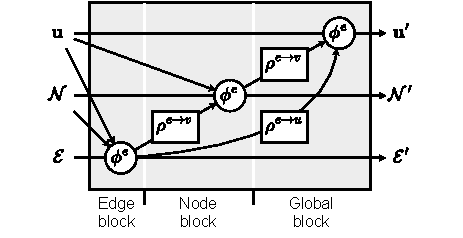
\includegraphics[width=\textwidth]{Figures/graph_networks/full_gn.pdf}
        \caption{Full GN Block}
        \label{fig:full_gn_block}
    \end{subfigure}
    \begin{subfigure}[b]{0.49\textwidth}
        \centering
        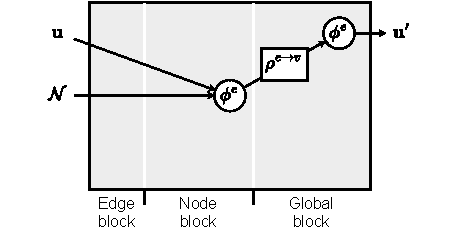
\includegraphics[width=\textwidth]{Figures/graph_networks/deepset.pdf}
        \caption{Deep Set}
        \label{fig:deep_set}
    \end{subfigure}
    \caption{Examples of different GN Block implementations \subref{fig:full_gn_block} A full GN Block has persistent edge and global features. \subref{fig:deep_set} A deep set only applies pooling to the node features to produce a global feature. Adapted from \textcite{RelationalInductiveBiases}.}
\end{figure}

\section{Transformers are Graph Networks}
\label{sec:transformers}

It is hard to overstate the impact of the transformer model~\cite{Attention} on deep learning.
Originally designed for NLP sequence-to-sequence tasks, transformers far surpassed the performance of all previous models, so much so that research in other sequence-based models, such as recursive neural networks, almost ceased entirely.
They also marked a massive leap in commercializing deep learning for NLP.
Starting in 2018, OpenAI began releasing the GPT~\cite{GPT} series of transformer models, arguably triggering a boom around large language models that continues to this day.
In 2019, Google announced that they were using the transformer-based BERT model~\cite{BERT} to power their search engine and transformers for their translation service.
In 2020, transformers were adapted to work on image data~\cite{VisionTransformer}, marking the point where transformers took the crown in computer vision benchmarks from CNNs as shown in \Cref{fig:benchmarks}.
Even image generation tasks that used to be dominated by UNets~\cite{Unet, DiffusionBeatsGANS} are now being performed by transformers~\cite{DIT, SD3}.
Transformers have become so ubiquitous that they are now considered the default choice for many deep learning tasks, regardless of the data type.

There are many variants for the transformer model, but they all share the same basic features.
Contrary to popular belief, these models do not natively run on sequences but on sets, and must be adapted to work on data with an inherent order.
We will focus on two main types of transformers, the transformer encoder and the transformer decoder.
The transformer encoder (TE) is a variant of the GN Block called a non-local neural network (NLNN)~\cite{NonlocalNeuralNetworks} as shown in \Cref{fig:transformer}.
This function operates on a pure set, with no persistent edge or global features.
It involves and message passing step equipped with an attention mechanism, followed by a node update step using an MLP\@.

The jargon of transformers differs slightly from that of GNNs.
Nodes are called tokens in many research papers on transformers.
The term attention is also used more broadly in transformers, not just referring to the means of weighting and aggregation, it is sometimes used to refer to the entire message passing step.
Furthermore, saying that a node attends to another is equivalent to saying that the node receives a message from another.
The adjacency matrix in a graph is also called the attention mask in a transformer.

\begin{figure}[h]
    \centering
    \begin{subfigure}[b]{0.49\textwidth}
        \centering
        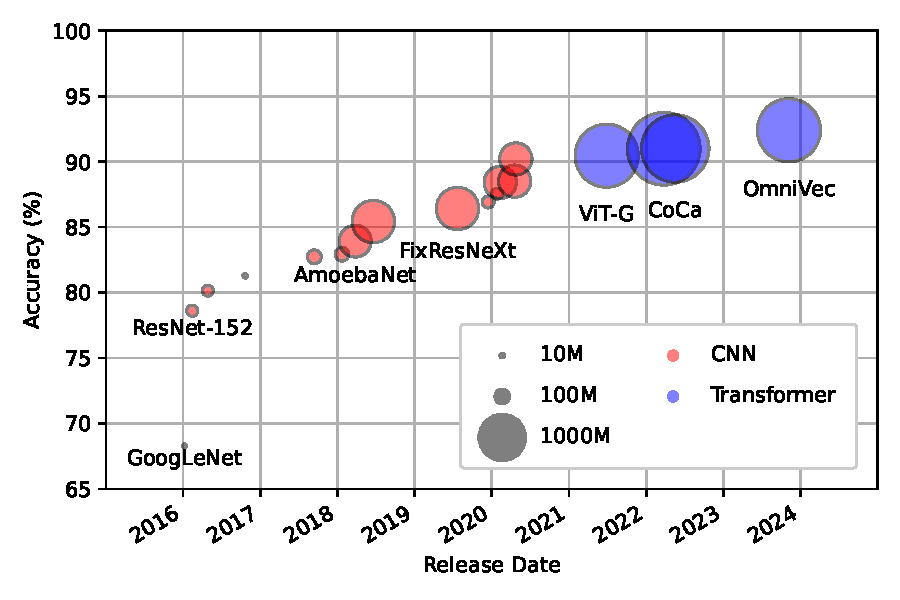
\includegraphics[width=\textwidth]{Figures/graph_networks/imagenet.pdf}
        \caption{}
        \label{fig:imagenet}
    \end{subfigure}
    \hfill
    \begin{subfigure}[b]{0.49\textwidth}
        \centering
        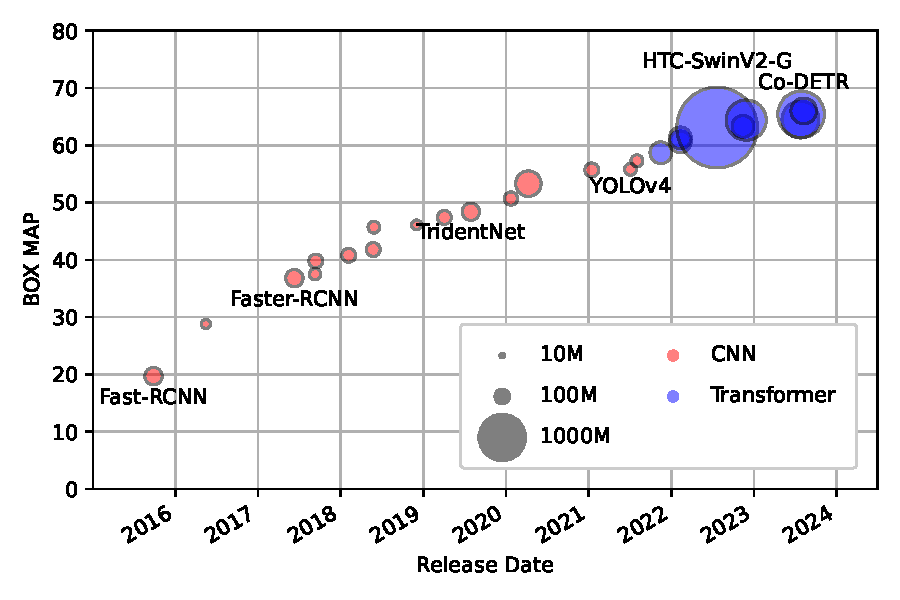
\includegraphics[width=\textwidth]{Figures/graph_networks/coco.pdf}
        \caption{}
        \label{fig:coco}
    \end{subfigure}
    \caption{Evolution of the state-of-the-art models in two common computer vision benchmarks~\cite{paperswithcode}. The size of the markers corresponds to the number of trainable parameters in the model. \subref{fig:imagenet} Accuracy on the ImageNet classification benchmark. \subref{fig:coco} Bounding box mean average precision (BOX MAP) the COCO object detection benchmark.}
    \label{fig:benchmarks}
\end{figure}

\begin{figure}
    \centering
    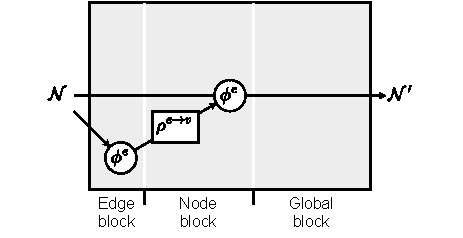
\includegraphics[width=0.49\textwidth]{Figures/graph_networks/nonlocal.pdf}
    \caption{NLNN / Transformer Encoder}
    \label{fig:transformer}
\end{figure}

\subsection{Transformer Attention is Just Message Passing}
\label{sec:attention}

There are many of ways to parameterize the message passing step in a GNN, and the one used in the transformer is the scaled dot-product attention (SDPA).
In SDPA, the message passed between nodes is a linear projection of the sender node attributes.
This means that each node sends out the same message to all of its neighbours called its \textit{value}, $\vert_{i} = \mathbf{W}^v \x_i$.
The message weight is based on a dot product between additional linear projections of the sender node, called they key \textit{key} $\k_{i} = \mathbf{W}^k \x_i$, and the receiver node, called the \textit{query} $\q_{j} = \mathbf{W}^q \x_j$.
Aggregation is simply a weighted mean of the incoming messages, where a softmax operation is applied to the attention logits to ensure that they sum to one.
To prevent the gradients from exploding, the attention logits are scaled by the square root of the dimensionality of the key and value tensors $d_k$.

In the framing of the GN Block, SDPA has the edge update is factorized into a tuple containing a scalar expressing the message weight $\alpha_k'(\x_{s_k}, \x_{r_k})$ and a vector function for calculating the message content $\mathbf{v}_k'(\x_{s_k})$.
Only $\alpha_k'$ depends on the pairwise interaction of both the sender and receiver nodes.
The pooling operation $\rho^{e \to x}$ normalizes over the receiver weights before aggregating the messages.
The block can be written as,
\begin{equation}
    \begin{aligned}
        \edge_k' &= \phi^e(\edge_k, \x_{s_k}, \x_{r_k}, \u)
        = ( a_k', \mathbf{v}_k' ) \\
        &= \left( \exp \left( \frac{1}{d_k} \mathbf{W}^q \x_{s_k} \cdot \mathbf{W}^k \x_{r_k} \right), \mathbf{W}^v \x_{s_k} \right), \\
        \mathbf{\bar\edge}_i &= \rho^{e \to x}(E_i) \\
       &= \frac{\sum_{k: r_k = i} a_k' \mathbf{v}_k'}{\sum_{k: r_k = i} a_k'},
    \end{aligned}
\end{equation}
for learnable weight matrices $\mathbf{W}^k \in \mathbb{R}^{d \times d_k}$, $\mathbf{W}^q \times \mathbb{R}^{d \times d_k}$, and $\mathbf{W}^x \in \mathbb{R}^{d \times d_v}$.

When using real values tensor representations, this operation can be done efficiently for all nodes in parallel using basic matrix operations.
Furthermore, it allows us to extend to two forms, self-attention and cross-attention, both expressible by the following equation,
\begin{equation}
    \label{eq:attention}
    \begin{aligned}
        \text{Attention}(\X_R, \X_S)
        &= \text{softmax}\left(\frac{(\X_S \mathbf{W}^q) (\X_R \mathbf{W}^k)^T}{d_k} + \mathbf{B}\right) \X_S \mathbf{W}^v, \\
        &= \text{softmax}\left(\frac{\mathbf{Q} \mathbf{K}^T}{d_k} + \mathbf{B}\right) \mathbf{V}.
    \end{aligned}
    \end{equation}
In this expression we distinguish between the tensor representing the sender nodes $\X_S \in \mathbb{R}^{N_S \times d}$ and the receiver nodes $\X_R \in \mathbb{R}^{N_R \times d}$.
Self-attention is where the sender and receiver set are the same $\X_S = \X_R$.
This is the standard message passing operation between nodes in a graph.
Cross-attention is where the sender set and receiver set are different $\X_S \neq \X_R$.
This operation is permutation invariant with respect to $\X_S$ and equivariant with respect to $\X_R$.
As shown by \Cref{fig:bipartite}, one can interpret this as the construction of a one-way bipartite graph between two sets, where all nodes in $\X_S$ send messages to all nodes in $\X_R$.
Note that the cardinality of the sender and receiver sets do not need to be the same.
Cross-attention is a powerful tool to condition one set on another and is used in many sequence to sequence tasks, from translation, to image captioning, and text-to-image generation.
Finally, the bias term $\mathbf{B}$ is a matrix of shape $(N_R, N_S)$ which can be used to focus or ignore certain pairs of nodes.

\begin{figure}
    \centering
    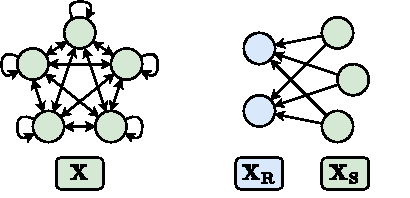
\includegraphics[width=0.5\textwidth]{Figures/graph_networks/bipartite.pdf}
    \caption{(left) Self-attention is standard message passing between all nodes in a graph. (right) Cross-attention creates a one-way bipartite graph between two sets of nodes.}
    \label{fig:bipartite}
\end{figure}

Transformers typically extend this operation to multi-headed attention (MHA), as shown in \Cref{fig:mha}.
This is where SDPA is performed $H$ times in parallel with different matrices $\mathbf{W}^q$, $\mathbf{W}^k$, $\mathbf{W}^v$, and $\mathbf{B}$.
The output of each head is concatenated and then mixed using a final linear layer,
\begin{equation}
    \begin{aligned}
    & \text{Head}_1 = \text{Attention}(\X_R, \X_S), \\
    & \text{Head}_2 = \text{Attention}(\X_R, \X_S), \\
    & \ldots, \\
    & \text{Head}_H = \text{Attention}(\X_R, \X_S), \\
    \vphantom{x} \\
    & \text{MHA}(\X_R, \X_S) = \text{Concat}(\text{Head}_1, \ldots, \text{Head}_H) \mathbf{W}^o.
    \end{aligned}
\end{equation}
In MHA, many types of messages are passed between the nodes and one can think of this as constructing a multi-graph on the set.
Both self- and cross-attention can be multi-headed where multi-headed self-attention (MHSA) is defined as $\text{MHSA}(\X) = \text{MHA}(\X, \X)$.

\begin{figure}
    \centering
    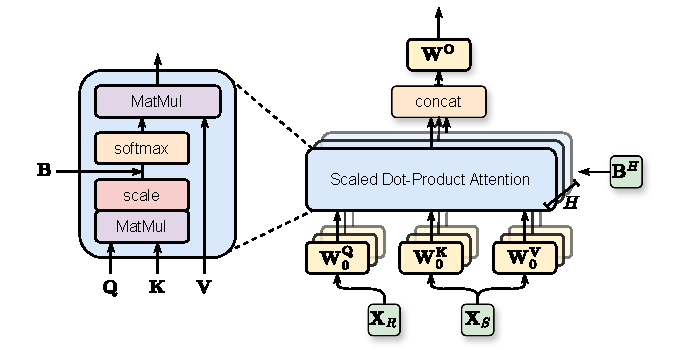
\includegraphics[width=0.8\textwidth]{Figures/graph_networks/mha.pdf}
    \caption{Multi-headed attention can be thought of as constructing a multi-graph with different edge types.}
    \label{fig:mha}
\end{figure}

\subsubsection{Implementing Multi-Headed Attention}

The dot product in the SDPA layer necessitates that the dimensions of key and query tensors are equal.
Additionally, the majority of SDPA implementations do not resize, resulting in $\mathbf{Q}$, $\mathbf{K}$, and $\mathbf{V}$ all having the same shape.
When extending to MHA, it is standard to split the dimensionality equally by the number of heads $H$.
This means that a single MHA function is typically parameterized by four square matrices corresponding to $4d^2$ learnable parameters with the number of heads $H$ being the sole hyperparameter of the block.

To enhance the model's expressivity, one can replace linear projections with affine transformations by including bias terms. However, it is important to note that the bias of the key operation is entirely redundant~\cite{RoleBiasTerms}.

Key to the success of transformers is the ease of implementation.
While many variants of GN Block block variants require custom libraries and are challenging to implement from scratch, MHA can be implemented in PyTorch using standard linear algebra operations, as demonstrated in \Cref{code:attention}.
All heads are computed in parallel using smart reshaping of the tensors.
This significantly simplifies the process of designing, building, testing, and exporting models.

While the message passing operation is considerably simpler than using MLPs for each stage as described in~\Cref{alg:gn_block}, it is possible to enhance the model's expressivity by scaling either the model dimension or the number of heads.
Contrary to popular belief, self-attention with these mechanisms does not require $O(N^2)$ memory complexity. There are algorithms available that achieve this without needing to manifest the full attention matrix~\cite{SelfattentionDoesNot, FlashAttentionFastMemoryEfficient}.

\begin{figure}
    \centering
    \scriptsize
    \begin{minted}{python}
    class Attention(nn.Module):
        def __init__(self, dim: int, num_heads: int):
            super().__init__()
            self.NH = num_heads
            self.HD = dim // num_heads
            self.scale = self.HD**-0.5
            self.wk = nn.Linear(dim, dim)
            self.wq = nn.Linear(dim, dim)
            self.wv = nn.Linear(dim, dim)
            self.wo = nn.Linear(dim, dim)

        def forward(self, xr: T.Tensor, xs: T.Tensor, bias: T.Tensor | int = 0) -> T.Tensor:
            q, k, v = self.wq(xs), self.wk(xr), self.wv(xs)              # project
            shape = (xr.shape[0], -1, self.NH, self.HD)                  # split heads
            q, k, v = (t.view(shape).transpose(1, 2) for t in (q, k, v))
            attn = (q @ k.transpose(-2, -1))                             # attention weight
            attn = (attn * self.scale + bias).softmax(dim=-1)
            x = attn @ v                                                 # aggregate
            x = x.transpose(1, 2).reshape(B, N, D)                       # mix heads
            return self.wo(x)
    \end{minted}
    \caption{A simple implementation of a multi-headed attention block in PyTorch.}
    \label{code:attention}
\end{figure}

% \subsubsection{Efficiency of Scaled Dot-Product Attention}

% SDPA stands out as an exceptionally efficient method for expressive message passing in fully connected graphs.
% To illustrate this, we can start by examining the simplest GNN variant, the GCN~\cite{GCN}, and identify its limitations.

% A single GCN layer, without normalization factors, can be expressed as,
% \begin{equation}
%     \begin{aligned}
%     \edge_k' &= \mathbf{W} \x_{s_k}, \\
%     \x_i' &= \sum_{k:r_k=i} \edge_k',
%     \end{aligned}
% \end{equation}
% for a single learnable weight matrix $\mathbf{W}$.
% Let us consider the shapes of the tensors in this operation.
% Representing the set of nodes as a real-valued tensor $\mathbf{X}$ of shape $(N, d)$, the operation can be performed using a matrix multiplication $\mathbf{W}: (N, d) \rightarrow (N, d)$, followed by a sum.

% In a fully connected graph, after one update step, every node would contain the same information, leading to an extreme case of over-smoothing.

% To avoid this over-smoothing, each message must be unique for each node pair.
% Thus, the challenge becomes finding the most efficient way to parameterize messages such that the output of the message constructing process is a tensor with shape $(N, N, d)$.
% Here we assume that the dimension of the nodes and the edges is the same.
% The first dimension in this tensor represents sender nodes, and the second dimension represents receiver nodes.
% The aggregation operation then acts over the first dimension to produce a tensor of shape $(N, d)$,
% \begin{align}
%     \text{construct method}: (N, d) & \rightarrow (N, N, d) \\
%     \text{aggregate}: (N, N, d) & \rightarrow (N, d).
% \end{align}

% The basic GN Block in \Cref{alg:gn_block} does this by concatenating the sender and receiver node attributes before passing them through an MLP\@.
% The operations and dimensions of the tensors of such a block are,
% \begin{align}
%     \text{concatenate}: (N, d) & \rightarrow (N, N, 2d) \\
%     \text{MLP}: (N, N, 2d) & \rightarrow (N, N, d) \\
%     \text{sum}: (N, N, d) & \rightarrow (N, d)
% \end{align}
% This meets the criteria for a highly expressive message passing operation, but it is not the most efficient, since a large tensor of shape $(N, N, 2d)$ is created and needs to be passed through a learnable operation, here an MLP.
% With very large graphs, we would like to avoid the construction of tensors with $O(N^2)$ elements.
% One way to mitigate this is to factorize the step into two learnable components, one to calculate the message weight (attention) and one to calculate the message content (value).

% Only one of these needs to be unique for each pairing and since the weight is a scalar and the content is a vector, it is much more efficient to allow the content to be degenerate.
% This is exactly the approach of GATs~\cite{GAT}, which perform the update,
% \begin{align}
%     \mathbf{W_1}&: (N, D)  \rightarrow (N, D) \\
%     \text{concatenate}&: (N, D)  \rightarrow (N, N, 2D) \\
%     \mathbf{W_2}&: (N, N, 2D)  \rightarrow (N, N) \\
%     \text{matrix multiply}&: (N, N), (N, D)  \rightarrow (N, D)
% \end{align}
% However, there is still the issue that this input and output of the learnable layers are $O(N^2)$.

% The $(N, N)$ matrix of attention weights needs to be learnable from the original $(N, D)$ node attributes and must be allowed to be unique for each pairing.
% Therefore, there must be a distinction between the sender and receiver nodes, this makes the required map $a: (N, D), (N, D) \rightarrow (N, N)$.
% There are few operations that can achieve this, and none so efficient as a dot product.
% Using linear projections for the initial embeddings means that the K, Q, V tensors can be computed in parallel.
% \begin{align}
%     \mathbf{W}: (N, D) & \rightarrow (N, 3D) \\
%     \text{split}: (N, 3D) & \rightarrow (N, D), (N, D), (N, D) \\
%     \text{scale-dot-softmax}: (N, D), (N, D) & \rightarrow (N, N) \\
%     \text{matrix multiply}: (N, N), (N, D) & \rightarrow (N, D)
% \end{align}
% While the other parts of the update do require $O(N^2)$ operations, crucially the input and output of the learnable layers dependent is only $O(N)$.

% The argument made here is that one will struggle to find a more simple and efficient way to parameterize the message passing step in a GNN that does not lead to over-smoothing when fully connected.
% The philosophy of the transformer is similar to the philosophy of composing MLPs from linear layers, in that the composition of simple, highly parameterized functions, is what provides expressivity.
% By and large the most complex component of the operation is the softmax function, but there exist algorithms to calculate this online without having to express the full attention matrix~\citetemp{FlashAttention}.
% Contrary to popular claims, self-attention with these mechanisms is non $O(N^2)$ in memory complexity~\citetemp{MemoryComplexity}.
% Some more recent models large models have even done away with the softmax, citing better performance beyond a certain model scale~\citetemp{Reformer, LinearAttetnion}.

\subsection{Transformer Variants}
\label{sec:transformer_variants}

There are numerous transformer variants, too many to cover in this thesis.
Common similarities exist among them, though terminology can be ambiguous and overlapping.
A single transformer block generally includes two types of sub-blocks: MHA for message passing and FFN/MLP layers for the node update.
These sub-blocks combine and repeat to form the larger transformer block.
MHA layers can be configured as self-attention or cross-attention, and are typically stacked with FFN layers in series~\cite{Attention}, but sometimes in parallel~\cite{Palm}.
Another distinguishing feature is the use of residual connections and normalization layers with various configuration options to stabilize training and prevent over-smoothing
Due to the wide range of transformer variants, empirical performance is often the guide for best practices.

Most transformer layers use an MLP with a single hidden layer that expands the node attributes' dimensionality by a factor of $M$.
However, modern transformers use Gated Linear Units (GLU)~\cite{GLU}, a network layer involving the element-wise multiplication of two linear projections, one of which is activated~\cite{SwiGLU},
\begin{equation}
    \text{FFN}_\text{SwiGLU}(\x_i) = \mathbf{W}_3(\text{Swish}(\mathbf{W}_1 \x_i + \mathbf{b}_1) \otimes (\mathbf{W}_2 \x_i + \mathbf{b}_2)) + \mathbf{b}_3.
\end{equation}
Many transformers also use the mixture-of-experts approach, where there exist many FFN layers, each with different parameters, and a gating mechanism to direct certain nodes to certain experts~\cite{MOE}.
Notably, while attention mechanisms are key to transformers' success, the majority of parameters are in these node update layers.

Residual connections are typically used to circumvent each sub-block.
The original transformer used a PostNorm configuration, where layer normalizations were applied after each residual connection~\cite{Attention}.
This was found to excessively squash the signal; therefore, contemporary transformers often utilize the PreNorm configuration~\cite{PreLN}.
Extra normalization within the sub-blocks is also common.

\subsubsection{Transformer Encoder}

A single PreNorm TE Block is shown in \Cref{fig:transformer_blocks}.
The update is given by,
\begin{equation}
\begin{aligned}
    \X & \leftarrow \X + \text{MSHA}(L_\text{norm}(\X)), \\
    \X & \leftarrow \X + \text{FFN}(L_\text{norm}(\X)).
\end{aligned}
\end{equation}
A full TE is composed of many TE Blocks stacked in series forming a permutation equivariant set to set transformation.
For many tasks, the TE is the main feature extractor.

\subsubsection{Transformer Decoder}

To condition the update of one set on another, a cross-attention (CA) block, can be utilized.
For a more expressive operation, the layer can include both self-attention and cross-attention, creating a transformer decoder (TD) block, as shown in \Cref{fig:transformer_blocks}.
The update of a TD block is written as,
\begin{equation}
\begin{aligned}
    \X_R & \leftarrow \X_R + \text{MHSA}(L_\text{norm}(\X_R)), \\
    \X_R & \leftarrow \X_R + \text{MHA}(L_\text{norm}(\X_R), \X_S), \\
    \X_R & \leftarrow \X_R + \text{FFN}(L_\text{norm}(\X_R)).
\end{aligned}
\end{equation}
The TE and TD are typically combined to create a set-to-set transformation that first extracts features from the input set, and the conditions the output set on these features.
This set-to-set transformation is the basis of many generative of sequence-to-sequence models.

\begin{figure}
    \centering
    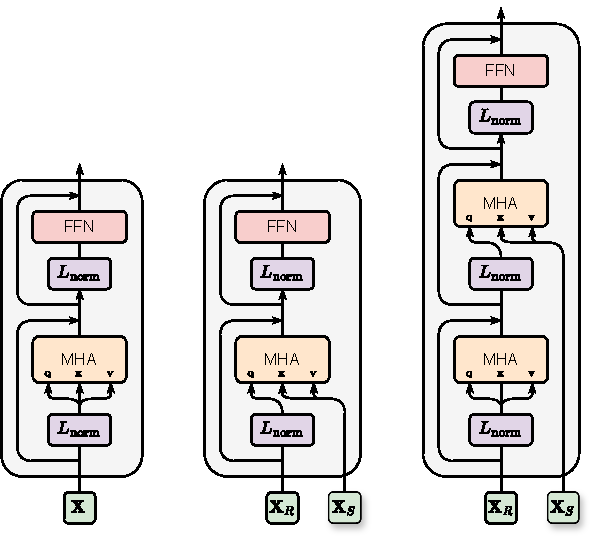
\includegraphics[width=0.7\textwidth]{Figures/graph_networks/transformer_variants.pdf}
    \caption{Some common transformer variants. (left) Transformer Encoder (TE) block. (center) Cross-Attention (CA) block. (right) Transformer Decoder (TD) block.}
    \label{fig:transformer_blocks}
\end{figure}

\subsection{Edge Attributes, Biases, and Sequences}
\label{sec:edge_biases_sequences}

When viewing the transformer as a GNN, the inclusion of edge information becomes intuitive.
For message passing on a single graph, if not represented sparsely, edge information is stored in a tensor $\edge \in \mathbb{R}^{N \times N \times d_e}$.
In the SDPA operation in \cref{eq:attention}, the attention matrix defined by,
\begin{equation}
    \mathbf{A} = \text{softmax}\left( \frac{\mathbf{Q} \mathbf{K}^T}{d_k} + \mathbf{B} \right),
\end{equation}
which has the shape $(N, N)$ for self-attention.
Extending this to MHA it gains an extra dimension $(N, N, H)$ aligning with the required shape of the edge tensor and making it the only valid candidate in the entire operation.
The query and key tensors $\mathbf{Q}$ and $\mathbf{K}$ stem from projections of the input, but $\mathbf{B}$ must have shape which is at least broadcastable to $(N, N, H)$.
Consequently, edge information can be integrated into a transformer through the bias term in the attention operation, a practice used in various scenarios.

The Particle Transformer (ParT)~\cite{ParticleTransformerJet} uses a TE to embed a set of particles, defined by their kinematics.
For each pair of particles, specific edge features are constructed using Lund Plane variables~\cite{LundJetPlane}.
The model uses an MLP to embed these edge features into a tensor of shape $(N, N, H)$, which becomes the attention bias in each of the TE Blocks.

The bias tensor is commonly set to negative infinity for specific node pairs and all heads, forcing the attention weight to zero after the softmax operation and eliminating the message weight. This allows the transformer to function on non-fully connected graphs without changing any of the underlying matrix operations.
It is also one of the main mechanisms for adapting the transformer to work on sequences, where the nodes are presented in a specific order.
By configuring the bias matrix as a lower triangular matrix with above-diagonal entries set to negative infinity, each node receives messages only from preceding nodes.
This technique, known as a causal masking, is used extensively in generative models as it lends itself to autoregressive sampling.
Causal masking allows for highly efficient training, as each stage of the autoregressive generation can be computed in a single forward pass.
Although generation requires sequential model execution, the training speed-up is a substantial benefit.
Many sequence generating models are called ``decoder only'', however in the presented framework, these models are TE models with a causal attention mask.

While a causal mask suffices for a transformer to grasp order~\cite{TransformerLanguageModels}, it is often complemented by \textit{positional encoding}.
Absolute positional encoding (APE) integrates sequence positions into node attributes.
A unique tensor $\mathbf{p}_i \in \mathbb{R}^{d}$ is constructed for each possible observed position $i$ and is added to the node attributes before the first transformer block, $\x_i \leftarrow \x_i + \mathbf{p}_i$.
Originally, fixed sinusoidal functions of varying frequencies encoded these positions, but recent models make $\mathbf{p}_i$ fully learnable~\cite{GPT}.
In images, APE, often termed spatial encoding, involves encoding and adding the 2D coordinates of a patch to its representation~\cite{VisionTransformer}.

APE is limited in capturing relative positions, necessitating the use of relative positional encoding (RPE)~\cite{SelfAttentionRelativePosition}.
RPE biases the attention matrix, serving as edge information, with various implementations.
$B$ can be parameterized as a learnable Toeplitz matrix, ALiBi~\cite{ALIBI} fixes the elements of this matrix to be simply $B_{ij} = m\times(i - j)$, for a fixed per-head scalar $m$, and rotary-positional-encoding rotates the query and key tensors by a fixed amount before the attention operation~\cite{RoFormerEnhancedTransformer}.

\subsection{Global Attributes and Conditioning Graph Updates}
\label{sec:global_attributes}

Global attributes are used to condition updates or can be used as outputs for graph-level tasks.
In \Cref{alg:gn_block}, the global attributes are updated by summing the node attributes which is then passed through an MLP\@.
However, a CA block provides a more expressive pooling operation, even when the cardinality of the receiving set is one.
This is known as class attention~\cite{GoingDeeper}, and is utilized in vision transformers for image classification.
These models typically have several TE layers for feature extraction, followed by a few CA layers to repeatedly pool the features into a single global attribute which is used for classification.

Global information can be redistributed to augment the message passing step by including them as inputs in the FFN layer~\cite{PCJeDiDiffusionParticle}.
More effectively, they can be used to perform adaptive normalization~\cite{FiLMVisualReasoning} and residual gating for each sub-block, a technique used in many state-of-the-art generative models~\cite{SD3, DIT, flux2024github}.
This is shown for a TE block in \Cref{fig:adaptive_gating} and can be written for a single sub-block $f$ as,
\begin{equation}
    \begin{aligned}
    & [\boldsymbol{\alpha}, \boldsymbol{\beta}, \boldsymbol{\gamma}] \leftarrow \text{MLP}(\u) \\
    & \X \leftarrow \X + \boldsymbol{\alpha} \otimes f \left(L_\text{norm}(\X)\boldsymbol{\gamma} \otimes  + \boldsymbol{\beta}\right).
    \end{aligned}
\end{equation}

\begin{figure}
    \centering
    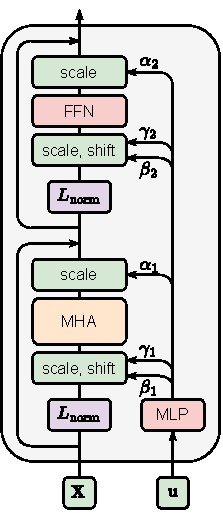
\includegraphics[width=0.25\textwidth]{Figures/graph_networks/adaptivegating.pdf}
    \caption{A TE block with adaptive normalization and gating to incorporate global information.}
    \label{fig:adaptive_gating}
\end{figure}

% 
\chapter{Flavour Tagging with Graph Networks and Transformers}
\label{ch:spice}

This chapter describes the design and implementation of several new GNNs and transformers for flavour tagging.
Jet flavour tagging is a crucial feature in many jet-based analyses at ATLAS, and an overview is provided in \Cref{sec:flavour_tagging}.
ATLAS uses dedicated algorithms to identify a jet's flavour, which corresponds to the flavour of the quark that initiated the jet, by analysing the properties of the associated charged particle tracks.
This task can be framed as a standard multi-class classification problem, making it particularly well-suited for deep learning.

The previous state-of-the-art flavour tagger used by the ATLAS experiment was GN1, a GNN that uses the GATv2 system of message passing~\cite{GATv2}.
In this section, two new models and their variants are introduced.
Each are GNNs with different architectures and mechanisms for message passing.
The first new model is called GN++ and is based on the complete GN Block architecture described in \Cref{sec:gn_block}, complete with persistent edge information and global attributes.
The second new model, Spice, is based on the transformer-encoder architecture described in \Cref{sec:transformer}.
Spice would turn out to be so performant and efficient that it would form the basis of the new GN2 flavour tagger adopted by the ATLAS collaboration~\cite{GN2Plots}.

One observation made during this project is that the field of machine learning moves is significantly faster compared to HEP.
Spice was being developed and presented to the flavour tagging group while GN1 was still undergoing calibration.
To address this rapid progression and prevent obsolescence, a major contribution of this thesis is the development of Salt~\cite{Salt}, a repository for the dedicated research, development, and deployment of deep learning algorithms for flavour tagging.
It ensures that the models used by the ATLAS collaboration remain up-to-date with the state-of-the-art models employed by the broader machine learning community.

\section{Datasets}

Training and evaluating GN++ and Spice requires the use of simulated datasets in order to provide a ground truth for the jet flavour.
This work reuses the same samples as the previous flavour taggers, DIPS and GN1, and further information can be found in \textcite{AlexThesis} and Ref.~\cite{GN1}.
The training datasets are selected to cover a wide range of $\pt$ values.
They are further resampled to ensure that the jet $\pt$ and $\eta$ distributions are nearly identical for the three jet flavours used in the classification, namely $b$-, $c$-, and light-jets.

Two simulated datasets are used.
The first dataset comprises $\ttbar$ events and covers the $20 < \pt < 250~\GeV$ phase space.
The simulation settings for this sample are derived from best fits of jet multiplicity and top quark momentum in data~\cite{ttbar1, ttbar2}.
The second dataset consists of $Z'$ events to enhance the training statistics in the high momentum phase space, $\pt > 250~\GeV$.
The $Z'$ boson is a non-SM particle, and its properties, such as its cross-section, are artificially adapted to produce a flat mass distribution, leading to a relatively uniform distribution of jets with $\pt$ up to $5~\TeV$.
The branching fractions are also adjusted to produce a roughly equal distribution of $b$-, $c$-, and light-jets.
The branching fractions of the $Z'$ boson are shown in \Cref{tab:zprime_branching} and the distributions of the jet $\pt$ and $\eta$ values are shown in \Cref{fig:jet_pt_eta}.

\begin{table}[ht]
    \centering
    \begin{tabular}{lr}
        \toprule
        Decay Mode     & Branching Fraction \\
        \midrule
        $b\bar{b}$     & 0.30               \\
        $c\bar{c}$     & 0.30               \\
        $s\bar{s}$     & 0.10               \\
        $d\bar{d}$     & 0.10               \\
        $u\bar{u}$     & 0.10               \\
        $\tau^-\tau^+$ & 0.05               \\
        $e^-e^+$       & 0.05               \\
        \bottomrule
    \end{tabular}
    \caption{Branching fractions for the $Z'$ boson \cite{Run2FTAlgs}.}
    \label{tab:zprime_branching}
\end{table}

\begin{figure}
    \centering
    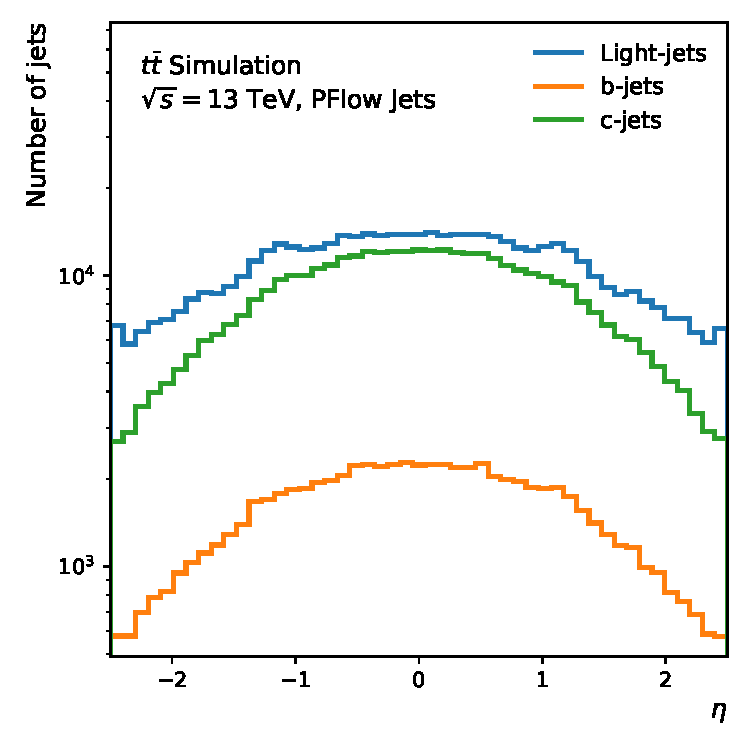
\includegraphics[width=0.45\textwidth]{figures/flavour_tagging/ttbar_0.pdf}
    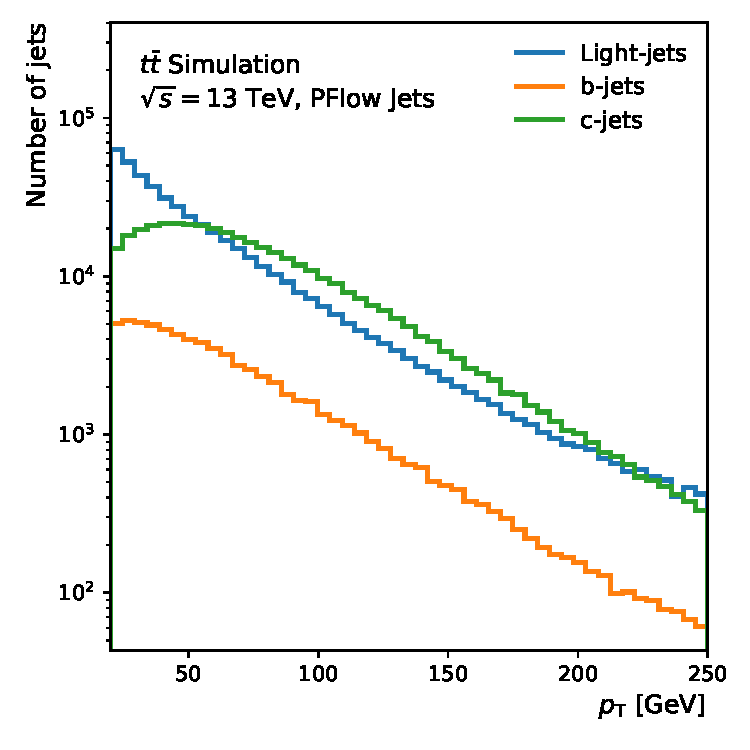
\includegraphics[width=0.45\textwidth]{figures/flavour_tagging/ttbar_1.pdf}
    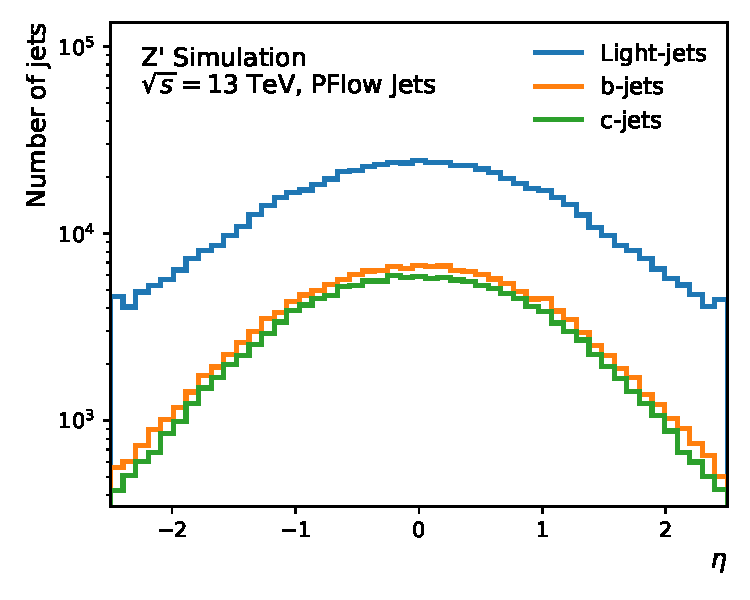
\includegraphics[width=0.45\textwidth]{figures/flavour_tagging/zprime_0.pdf}
    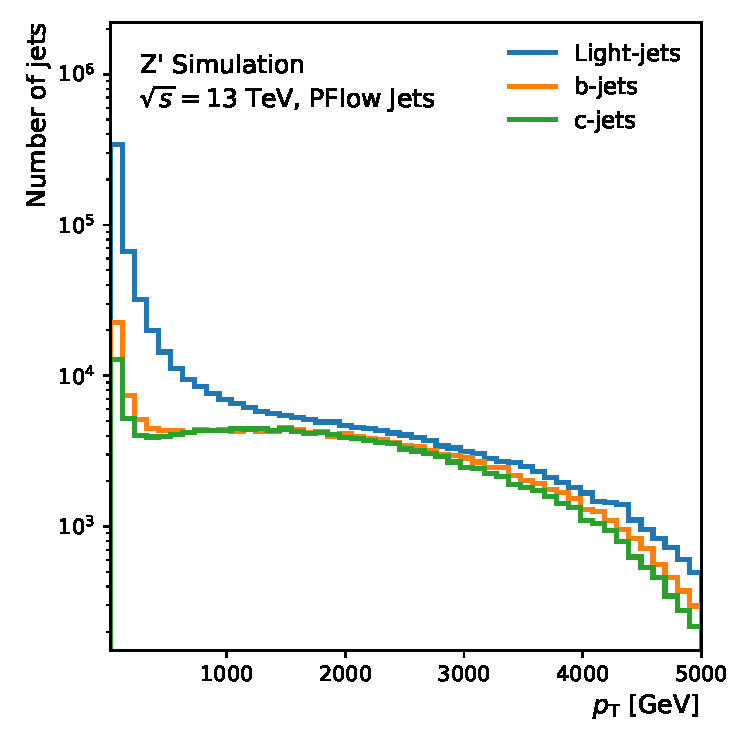
\includegraphics[width=0.45\textwidth]{figures/flavour_tagging/zprime_1.pdf}
    \caption{Original jet $\pt$ (left) and $\eta$ (right) distributions for the $\ttbar$ (top) and $Z'$ (bottom) training datasets. Plots were created using a representative sample.}
    \label{fig:jet_pt_eta}
\end{figure}

\subsection{Monte Carlo Generation}

Simulated proton-proton collisions initiate both datasets at a centre-of-mass energy of $\sqrt{s} = 13~\TeV$.
Hard-scatter events for the $\ttbar$ sample are generated at next-to-leading order using \powheg v2~\cite{Powheg1, Powheg2, Powheg3}.
These events are interfaced with \pythia 8.230~\cite{Pythia8} using the \textsc{A14} tune~\cite{A14} to perform parton showering and hadronization.
For the parton distribution functions, the \textsc{NNPDF3.0NNLO}~\cite{PDF3.0} set is used for matrix element calculations, while the \textsc{NNPDF2.3LO}~\cite{PDF2.3} set is used for showering.
The cut-off scale parameter for the first-gluon-emission $h_{\text{damp}}$ is set to 1.5 times the top quark mass of $m_t = 172.5~\GeV$.
The $Z'$ sample is generated and showered using \pythia 8.212 with the \textsc{A14} tune and the \textsc{NNPDF2.3LO} set of parton distribution functions.
The flat mass distribution of the $Z'$ boson is achieved by applying a per-event weight to broaden the natural decay width of the $Z'$ boson.

Decays of $b$- and $c$-hadrons are simulated using the \textsc{EvtGen v1.6.0} package \cite{EvtGen}.
The detector response is performed using the \geant simulation package~\cite{Geant4} with the ATLAS simulation setup~\cite{ATLASSim}.
Interactions with heavy flavour hadrons and the detector material are not simulated but accounted for in correction factors and systematic uncertainties.
Pileup is modelled by overlaying extra minimum bias events using the \pythia 8.160 generator with the \textsc{A3} tune~\cite{A3} and the \textsc{NNPDF2.3LO} parton distribution functions.
Pileup and hard-scatter signals are combined during the digitization step of the simulation.
In-time pileup is modelled using an average of 40 interactions per bunch crossing, while out-of-time pileup is modelled using bunch crossings before and after the primary interaction.

\subsection{Reconstruction}

The simulation output is reconstructed using the standard ATLAS reconstruction procedure described in \Cref{sec:event_reconstruction}.
For all models described in this chapter, the inputs are the tracks associated with the jet and no calibrated physics objects, such as photons, electrons, or muons, are used.

Charged particle tracks are required to pass the loose selection criteria~\cite{DL1D} as shown in \Cref{tab:track_loose}.
The primary vertex (PV) is the vertex with the highest sum of squared transverse momenta of the associated tracks.
The impact parameters (IPs) for each track is measured with respect to the PV of the event.
Jets are reconstructed from particle-flow objects~\cite{PFlow} using the anti-$k_t$~\cite{AntiKt} algorithm with a radius parameter of $R = 0.4$.
More details can be found in \Cref{sec:jets_reconstruction}.
Tracks are associated to a jet based on the $\Delta R$ separation to the jet axis.
The threshold for association decreases as a function of the jet $\pt$ to account for the increased collimation of the jet cone, from $\Delta R = 0.45$ at $\pt = 20~\GeV$ to $\Delta R = 0.25$ at $\pt \geq 200~\GeV$.
A track is always associated to the jet with the smallest $\Delta R$ separation.

\begin{table}
    \centering
    \begin{tabular}{lr}
        \toprule
        Variable                              & Requirement \\
        \midrule
        $\pt$                                 & $> 1~\GeV$  \\
        $d_0$                                 & $< 3.5~\mm$ \\
        $z_0 \sin \theta$                     & $< 5~\mm$   \\
        Number of hits in the SCT             & $\geq 8$    \\
        Number of hits shared by other tracks & $\leq 2$    \\
        Number of holes in the SCT            & $\leq 3$    \\
        Number of holes in the pixel detector & $\leq 2$    \\
        \bottomrule
    \end{tabular}
    \caption{Loose selection criteria for charged particle tracks~\cite{DL1D}. A hole is defined as a missing hit in a layer where one is expected.}
    \label{tab:track_loose}
\end{table}

\subsection{Truth Labelling}

As with GN1, these networks are trained to perform three complementary tasks.
The primary task is to classify the jet flavour.
The first \textit{auxiliary} task is to predict the origin of each track within the jet.
The second \textit{auxiliary} task is to segment the jet: given any two tracks, determine if they emerged from the same vertex.
Each of these requires defining ground truth labels from the simulation.

For the primary task, the truth labels of the jets stem from the existence of generator level particles within a $\Delta R$ separation of 0.3.
The jet is associated with the particle with the highest priority within this radius.
The considered particles in order of decreasing priority are, $b$-hadrons, $c$-hadrons, and $\tau$ leptons, which result in the jet being labelled as a $b$-jet, $c$-jet, $\tau$-jet respectively.
If no such particles are found, the jet is labelled as a light-jet.
Jets found to be caused by $\tau$ lepton decays are discarded for this study.

The labels for the track origin are derived by matching the reconstructed track hits to the simulated hits a particle made during the \geant simulation.
This matching criterion is performed using the~\textit{truth-matching probability} (TMP)~\cite{PerformanceATLASTrack}.
This is the ratio of number of matched hits to the total number of hits in the track, with added factors to account for the varying efficiencies of the pixel detector, SCT, and TRT\@.
Each track is associated with the truth particle with the highest TMP\@.
If no truth particle results in a TMP greater than 0.75, the track is labelled as ``Fake'' as it is likely to have been reconstructed from signals produced by multiple overlapping particles.
Once the track is associated with a truth particle, it is classified based on the truth particle's origin.
This results in eight possible classes which are shown in \Cref
{tab:track_labels}.

Finally, the truth vertex labels are binary, indicating whether a pair of tracks emerged from the same secondary vertex within the jet.
The label does not depend on the ordering of the pair, and self-pairs are not considered.
Thus, for a jet with $N$ tracks, there are $N(N-1)/2$ vertex labels.
The label is only set to True if the associated truth particles of each track share an origin within $1~\mm$ of each other.
If one of the tracks is labelled as ``Fake'' or from a pileup interaction, the pair is always labelled False.

\begin{table}
    \centering
    \begin{tabular}{rl}
        \toprule
        Class & Description                                                       \\
        \midrule
        1     & From a $b$-hadron decay                                           \\
        2     & From a $c$-hadron decay which itself originated from a $b$-hadron \\
        3     & From a $c$-hadron decay not originating from a $b$-hadron         \\
        4     & From a $\tau$-lepton decay                                        \\
        5     & From other secondary decays such as kaons                         \\
        6     & From the primary vertex                                           \\
        7     & From a pileup $pp$ interaction                                    \\
        8     & A ``Fake'' track from multiple overlapping particles              \\
        \bottomrule
    \end{tabular}
    \caption{The eight possible classes for each track based on the origin of the associated truth particle.}
    \label{tab:track_labels}
\end{table}

\subsection{Selection and Sampling}

Jets are required to have $\pt > 20~\GeV$ and $|\eta| < 2.5$ and may not overlap with a generator-level lepton from a $W$ or $Z$ decay.
For the $Z'$ sample, jets must have $\pt > 250~\GeV$ to avoid simulation artefacts.
All jets with $\pt < 60~\GeV$ and $|\eta| < 2.4$ must also pass the tight working point of the JVT algorithm in order to minimize contributions from pileup~\cite{JVT}.

As shown in \Cref{fig:jet_pt_eta}, there is a significant difference between the jet $\pt$ and $\eta$ distributions for the three jet flavours and the two simulated datasets.
This discrepancy would bias the model's training and lead to issues for its implementation.
To mitigate this, the training dataset is resampled with replacement to ensure that the 2D distribution of jet $\pt$ and $\eta$ is identical for the three jet flavours~\cite{AlexThesis}.
After resampling, the training set contains a total of 120 million jets split equally between the three classes.
The composition of the training set is around 70\% $\ttbar$ and 30\% $Z'$ jets.
The distributions of the jet $\pt$ and $\eta$ for the resampled datasets are shown in \Cref{fig:train_jet_pt_eta}.
During training, 5\% of jets are reserved for hold out cross validation.

Two statistically independent test samples are also produced to evaluate the tagging algorithms.
After applying the same selection criteria, these test sets contain 1 million $\ttbar$ and $Z'$ jets, respectively.
No resampling is applied to the test datasets.

\begin{figure}
    \centering
    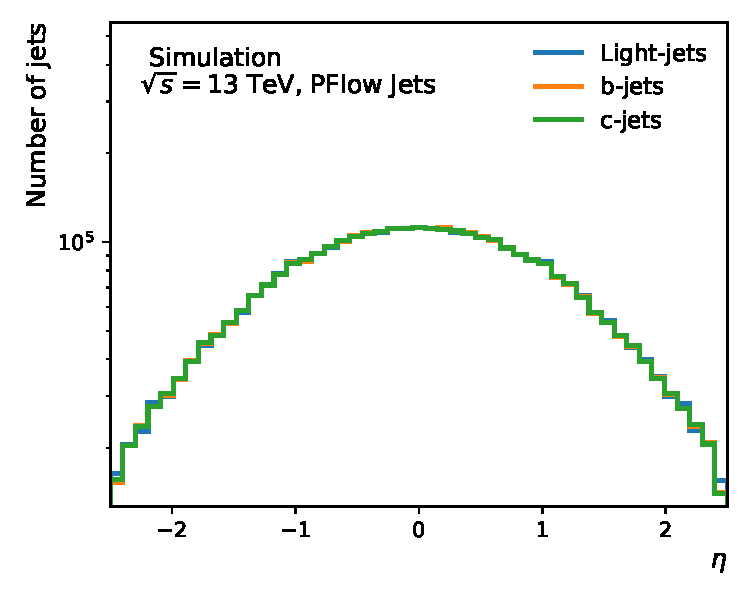
\includegraphics[width=0.45\textwidth]{figures/flavour_tagging/train_0.pdf}
    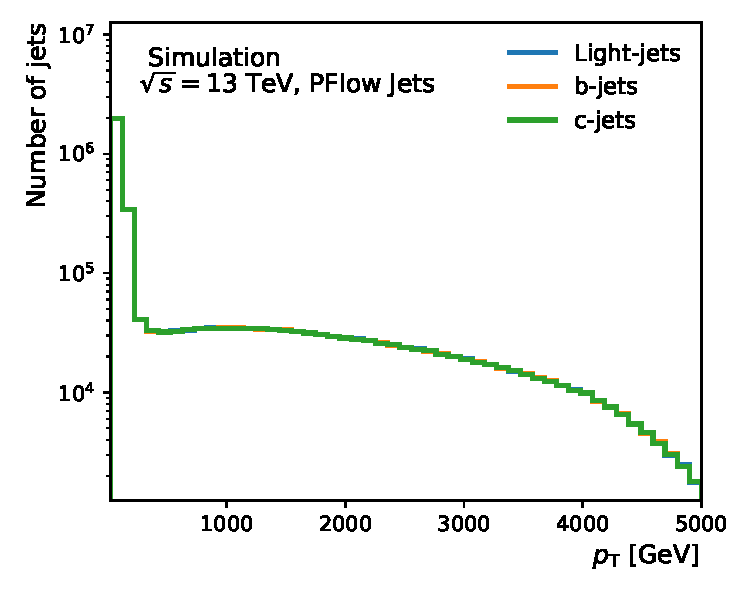
\includegraphics[width=0.45\textwidth]{figures/flavour_tagging/train_1.pdf}
    \caption{Resampled jet $\pt$ (left) and $\eta$ (right) distributions for the training dataset. For these plots only 10M jets were selected as a representative sample.}
    \label{fig:train_jet_pt_eta}
\end{figure}

\subsection{Input Features}

The inputs to all models presented in this chapter are the same as those used in GN1.
They include two kinematic jet variables, $\pt$ and $\eta$, and up to 40 tracks associated with the jet.
Each track is represented by a vector containing 21 features, detailed in \Cref{tab:track_features}.
The impact parameter significances are calculated by dividing the measured value by its estimated uncertainty.
Almost all $\ttbar$ jets contain less than 40 tracks, but a non-negligible fraction of $Z'$ jets contain more, as shown in \Cref{fig:track_multiplicity}.
For these jets, only the 40 tracks with the highest transverse IP significance $s(d_0)$ are retained.
All features are preprocessed via standardization to have zero mean and unit variance based on the training set statistics.

\begin{figure}
    \centering
    \includegraphics[width=0.45\textwidth]{figures/flavour_tagging/ttbar_2.pdf}
    \includegraphics[width=0.45\textwidth]{figures/flavour_tagging/zprime_2.pdf}
    \caption{Original non-resampled number of tracks associated with each jet in the $\ttbar$ (left) and $Z'$ (right) datasets.}
    \label{fig:track_multiplicity}
\end{figure}

\begin{table}[h]
    \centering
    \begin{tabular}{ll}
        \toprule
        \midrule
        \multicolumn{2}{c}{Jet level inputs}                                                    \\
        \midrule
        $\pt$             & Jet transverse momentum                                             \\
        $\eta$            & Signed jet pseudorapidity                                           \\
        \midrule
        \midrule
        \multicolumn{2}{c}{Track level inputs}                                                  \\
        \midrule
        $q/p$             & Track charge divided by momentum                                    \\
        $\Delta\eta$      & Pseudorapidity of the track relative to the jet $\eta$              \\
        $\Delta\phi$      & Azimuthal angle of the track relative to the jet $\phi$             \\
        $d_0$             & Closest distance from the track to the PV in the longitudinal plane \\
        $z_0 \sin \theta$ & Closest distance from the track to the PV in the transverse plane   \\
        $\sigma(q/p)$     & Uncertainty on q/p                                                  \\
        $\sigma(\theta)$  & Uncertainty on track polar angle $\theta$                           \\
        $\sigma(\phi)$    & Uncertainty on track azimuthal angle $\phi$                         \\
        $s(d_0)$          & Lifetime signed transverse IP significance                          \\
        $s(z_0)$          & Lifetime signed longitudinal IP significance                        \\
        nPixHits          & Number of pixel hits                                                \\
        nSCTHits          & Number of SCT hits                                                  \\
        nIBLHits          & Number of IBL hits                                                  \\
        nBLHits           & Number of B-layer hits                                              \\
        nIBLShared        & Number of shared IBL hits                                           \\
        nIBLSplit         & Number of split IBL hits                                            \\
        nPixShared        & Number of shared pixel hits                                         \\
        nPixSplit         & Number of split pixel hits                                          \\
        nSCTShared        & Number of shared SCT hits                                           \\
        nPixHoles         & Number of pixel holes                                               \\
        nSCTHoles         & Number of SCT holes                                                 \\
        \bottomrule
    \end{tabular}
    \caption{Input features for the GNN flavour taggers~\cite{GN1}.}
    \label{tab:track_features}
\end{table}

\section{Model Design}

All proposed models in this chapter can be considered as extensions of GN1.
Both Spice and GN++ adhere to a similar framework as GN1, but incorporate advancements in message passing techniques and contemporary architectural trends.
Following the description of the GN Block, as introduced in~\textcite{RelationalInductiveBiases}, features such as persistent edge information, persistent global information, and dedicated node updates are tested.
The transformer architecture is also explored, which uses scaled dot-product attention (SDPA), covered in \Cref{sec:transformers}, to perform message passing.
Other aspects of modern network design, such as PreNorm and residual additive connections are also incorporated.

GN1 introduced the idea of a monolithic graph neural network which would simultaneously perform jet tagging, track identification, and vertexing matching.
Framing the input data as a graph from \Cref{sec:graph_definition},the set of tracks associated with the jet are the nodes $\mathcal{N}$, and the associated jet kinematics are the global attributes $\u$.
In this context, there is no explicit graph structure (adjacency matrix) or edge features, although one can include them by deriving attributes from pairs of tracks.
The three training objectives are equivalent to performing a graph-level task, a node-level task, and an edge-level task simultaneously.
Thus, one can think of these models as mappings from the graph structure $(\mathcal{N}, \emptyset, \u) \rightarrow (\mathcal{N}', \mathcal{E}', \u')$, and the loss is calculated on each of the three outputs.

While the edges are featureless, all models treat the graph as fully connected, allowing each node to send and receive messages from all others.
Self-loops are also permitted.
This fully connected approach is found to be beneficial for performance while not significantly increasing the computational cost as the maximum cardinality of the graph (40) is relatively low compared to other graph-based tasks in machine learning.

To compare the information flow within the layers of GN1, the GN++ models, and Spice, the flowcharts in \Cref{fig:gn1_graph}, \Cref{fig:gnpp_graph}, \Cref{fig:gna_graph}, and \Cref{fig:spice_graph} are used.
These diagrams share similarities with the illustrations of the GN Block \Cref{fig:gn_block} but explicitly display the tensor operations acting on each attribute.
The key for each operation is shown in \Cref{fig:key}.

\begin{figure}[h!]
    \centering
    \includegraphics[width=0.99\textwidth]{figures/flavour_tagging/key.pdf}
    \caption{Key for the flowcharts of the GNN operations.}
    \label{fig:key}
\end{figure}

\subsection{GN1}
\label{sec:gn1}

The specifics of the GN1 model are described to better highlight the changes introduced in the GN++ and Spice models.
Here, the original GN1 implementation~\cite{GN1} is used, which is distinct from later variants~\cite{SamThesis} that adopted transformer-like features partly as a result of the success of Spice.
A diagram of the GN1 model is shown in \Cref{fig:gn1}.

The model begins with the track initializer, an MLP that individually projects the track features into 64 dimensional node embeddings.
The initializer also takes the jet kinematics as extra context information.
These nodes then passed through a series of GATv2 layers~\cite{GATv2}, each updating the features by aggregating information from all other nodes.
Within each GATv2 layer the there exists a learnable square matrix $\W$, which is used to simultaneously calculate the message sent between each node pair as well as the message weight using,
\begin{align}
    \vert_{ij} & = \W \x_i,                                                                     \\
    e_{ij}     & = \text{softmax}_i\left(\ba \cdot \relu\left([\W \x_i, \W \x_j]\right)\right).
\end{align}
Here, $\vert_{ij}$ is the message sent from node $i$ to node $j$,
$e_{ij}$ is the aggregation weight of that message and $\ba$ is a learnable vector.
A softmax is applied to ensure the total weight of all incoming messages to each node sums to one.
The messages are then summed to update the node information across the graph,
\begin{equation}
    \x_j' = \relu\left(\sum_{i} e_{ij} \vert_{ij}\right).
\end{equation}

GN1 uses three of these GATv2 layers to build its central feature extractor.
The final node features $\{\x_i'\}_{i=1}^{N}$ are then aggregated using a weighted sum to create a pooled graph representation,
\begin{equation}
    \con = \sum_{i} \text{softmax}_i\left(\bias \cdot \x_i'\right) \x_i',
\end{equation}
where $\bias$ is a learnable vector.
The tensor $\con$ is passed through an MLP to produce an output of size 3, which can be used for the graph-level classification task.
For the node-level task, final node features are each concatenated with $\con$ and passed through another MLP with 8 outputs.
For the edge-level task, all possible pairs of nodes are concatenated, not including self-pairs, and passed through a third MLP with a single output.
In total GN1 has 820k trainable parameters with many of them being located in these three output MLPs and the track initializer.
The model was implemented using the PyTorch Geometric library~\cite{PYG}.

A schematic diagram of the GATv2 layers that make up the GN1 tagger is shown in \Cref{fig:gn1_graph} which highlights some possible inefficiencies.
These layers reuse the same projection matrix $\W$ to calculate both the message content and weight, and it is probable that these distinct operations could be better performed with dedicated projections.
Notably missing are any strong node updates after the message passing step.
Framing this in the context of the GN Block means that the node update $\phi^x$ is simply an elementwise ReLU activation function.
Finally, there is little to prevent oversmoothing in the node features, which may indicate why GN1 was limited to three layers and was fairly reliant on the auxiliary tasks to improve performance.

\begin{figure}[h]
    \centering
    \includegraphics[width=0.99\textwidth]{Figures/cern_atlas/GN1.png}
    \caption{Schematic diagram of the GN1 model from Ref.~\cite{GN1}.}
    \label{fig:gn1}
\end{figure}

\begin{figure}
    \centering
    \includegraphics[width=0.99\textwidth]{figures/flavour_tagging/gn1.pdf}
    \caption{Diagram of the operations within a GATv2 layer~\cite{GATv2} used by GN1.}
    \label{fig:gn1_graph}
\end{figure}

\subsection{GN++}
\label{sec:gnp}

The GN++ model is based on the complete GN Block architecture described in \Cref{sec:gn_block}.
The only omission is the lack of a $\rho^{e \to u}$ pooling operation as it was found to be computationally expensive while offering no performance benefit.
This model is designed to be a more expressive graph network than GN1.
While each layer of GN1 essentially operates on a set $\mathcal{N}$, GN++ operates on a graph $(\mathcal{E}, \mathcal{N}, \u)$ with fully defined nodes, edges, and global attributes.
This model is built using a modular custom graph library for PyTorch.
Each of the operations within the GN Block could be easily deactivated allowing rapid design experimentation.
The best-performing model uses persistent edge features, persistent global features, layer normalization applied to the inputs of each learnable sub-layer, residual connections around each update, and multi-headed attention.
A diagram of the information flow in a single of these layers is shown in \Cref{fig:gnpp_graph}, and pseudocode for the update is shown in \Cref{alg:gnpp}.

\begin{figure}[h!]
    \centering
    \includegraphics[width=0.99\textwidth]{figures/flavour_tagging/gnpp.pdf}
    \caption{Diagram of the operations within layer of the GN++ tagger.}
    \label{fig:gnpp_graph}
\end{figure}

\begin{algorithm}[h!]
    \caption{The full GN++ block. All weight calculations are followed by a softmax operation and square brackets denote concatenation.}
    \label{alg:gnpp}
    \begin{algorithmic}[1]
        \State \textbf{Input:} Graph attributes $\mathcal{G} = (\mathcal{N}, \mathcal{E}, \u)$
        \State \textbf{Output:} Updated graph attributes $\mathcal{G}' = (\mathcal{N}', \mathcal{E}', \u')$
        \For{each edge $\edge_k$ in $\mathcal{E}$}
        \State $\edge_k' \gets \text{MLP}_e(\lnorm[\edge_k, \x_{s_k}, \x_{r_k}, \u]) + \edge_k$ \Comment{residual update to edge features}
        \State $\w_k \gets \text{MLP}_{e \to x}(\lnorm[\edge_k, \x_{s_k}, \x_{r_k}, \u])$ \Comment{calculate edge weights}
        \EndFor
        \For{each node $\x_i$ in $\mathcal{N}$}
        \State $\mathbf{\bar\edge}_i \gets \sum_{k: r_k = i} \w_k \edge_k'$ \Comment{attention pool edges}
        \State $\x_i' \gets \text{MLP}_v(\lnorm[\mathbf{\bar\edge}_i, \x_i, \u]) + \x_i$ \Comment{residual update to node features}
        \State $\w_i \gets \text{MLP}_{x \to u}(\lnorm[\mathbf{\bar\edge}_i, \x_i, \u])$ \Comment{calculate node weights}
        \EndFor
        \State $\mathbf{\bar{x}} \gets \sum_{i} \w_i \x_i'$ \Comment{attention pool nodes}
        \State $\u' \gets \text{MLP}_u(\lnorm[\mathbf{\bar{x}}, \u]) + \u_i$ \Comment{residual update to global attributes}
    \end{algorithmic}
\end{algorithm}

In a single layer, there are 5 MLPs: 3 to perform the updates $\phi^x$, $\phi^e$, and $\phi^u$, and two to calculate the attention weights for the $\rho^{e \to x}$ and $\rho^{x \to u}$ steps.
Multi-headed attention is achieved by having multiple outputs for the $\rho^{e \to x}$ and $\rho^{x \to u}$ MLPs, and each is softmaxed separately.
Four attention heads are used for the multi-headed experiments.
All updates are additive residuals, and the weights of the final layer of each update MLP are initialized with zeros to ensure they layer starts as the identity function.
All but the final MLPs in the model are non-resizing, and contain a single hidden layer with double the dimension of the input and a LeakyReLU activation function.

A basic linear projection is used for the track initializer instead of the full MLP used in GN1.
Edges and global information are treated as empty for the first layer, after which they are described with the same dimension as the node features.
The three networks for the graph, node, and edge level tasks are no longer required, as the GN Block already has outputs for each level.
The output dimension of the final update MLPs is set to match the required dimension of each task.
The residual connections in this final GN Block are each passed through a linear resizing layer to match the output dimension.
Five graph layers are used in total, each with half the embedding dimension of GN1, resulting in roughly 780k trainable parameters, slightly less than GN1.

Each of the features of the GN++ model can be deactivated to investigate their impact on performance.
The minimal model, which we call GNA, is shown in \Cref{fig:gna_graph}, and it is close to, but not exactly the same, as GN1.
This provides a good baseline upon which we can iteratively add complexity.

\begin{figure}[h!]
    \centering
    \includegraphics[width=0.99\textwidth]{figures/flavour_tagging/gna.pdf}
    \caption{Diagram of the operations within one layer of the GNA tagger.}
    \label{fig:gna_graph}
\end{figure}

\subsection{Spice}

The Spice model is based on the transformer-encoder architecture described in \Cref{sec:transformer_variants}.
The full model is shown in \Cref{fig:spicefull}.
As a transformer, each layer does not produce or retain edge features, only operating on the set of nodes using multi-headed self-attention to perform message passing.

\begin{figure}[h!]
    \centering
    \includegraphics[width=0.99\textwidth]{figures/flavour_tagging/spice_full.pdf}
    \caption{Diagram of the full Spice tagger.}
    \label{fig:spicefull}
\end{figure}

Comparatively, the layer structure of the TE Block is significantly simpler than the GN Block, only requiring four linear layers and a single MLP\@.
The information flow diagram is shown in \Cref{fig:spice_graph}.
Like GN++, the model is equipped with MLPs for strong node updates, which double the hidden dimension of the nodes.
The best performance was found using four attention heads.

To construct the pooled graph representation $\con$, three CA Blocks with four attention heads to send messages from each track onto a single learnable class token~\cite{GoingDeeper}.
This process allows the model to decide on a jet-by-jet basis what information to request from the tracks to assist with classification.
Like GN1, three separate MLPs perform the graph-, node-, and edge-level tasks.
These three MLPs and the track initializer are much smaller than the ones used in GN1, which reduces the number of parameters in the model.

To ensure a fair comparison, Spice has roughly the same number of trainable parameters as GN1.
Spice's primary hyperparameters are the embedding dimension and the number of TE Blocks which are set to 64 and 7, respectively, resulting in a model with 800k trainable parameters.
The model is implemented using standard PyTorch operations and is thus conceptually easier to work with than both GN++ and GN1.

\begin{figure}[h!]
    \centering
    \includegraphics[width=0.99\textwidth]{figures/flavour_tagging/spice.pdf}
    \caption{Diagram of the operations within one TE layer of the Spice tagger. The multiple attention heads are not shown for clarity.}
    \label{fig:spice_graph}
\end{figure}

\section{Training}

The same training loss as GN1 is used for all models, involving a weighted sum of three loss terms,
\begin{equation}
    \mathcal{L} = \mathcal{L}_{\text{graph}} + \alpha \mathcal{L}_{\text{node}} + \beta \mathcal{L}_{\text{edge}}.
\end{equation}
The graph loss $\mathcal{L}_{\text{graph}}$ is a cross-entropy loss between the predicted jet flavour and the ground truth.
The node loss $\mathcal{L}_{\text{node}}$ is calculated similarly but for the track origin task and averaged over all tracks in the jet.
The edge loss $\mathcal{L}_{\text{edge}}$ is calculated using a binary cross entropy between the predicted vertex label and the ground truth.
These additional loss terms help steer the model to learn jet representations linked to the physics related to the jet's flavour.
By predicting the true origin of each track and the vertex compatibility of each track-pair the model is actively looking for displaced vertices and thus heavy flavour decays.
These auxiliary training objectives are viewed as ``stepping stones''~\cite{GN1} on the way to determining the flavour of the jet.

Before averaging across the batch, the auxiliary loss terms were multiplied by a per sample weight.
The node task is weighted by the inverse frequency of each category in \Cref{tab:track_labels} found in the training set to account for class imbalance.
The weight for each pair of tracks in the edge task is set to two if the track pair is from a $b$- or $c$-hadron decay and one otherwise.
This reweighting forces the model to focus on heavy flavour vertices, which are more significant for flavour tagging.
No balancing is required for $\mathcal{L}_{\text{graph}}$ due to the resampling of the training set.
Averaging over all jets in the batch does mean that jets with more tracks contribute more to the gradients due to more terms in the track and edge loss, but this effect is minimal.

For the main models, the same loss coefficients as GN1, $\alpha = 0.5$ and $\beta = 1.5$.
Ablation studies are also run where $\alpha$ and $\beta$ is set to zero to determine the effect of the auxiliary tasks on the model's flavour tagging performance.

The training configuration for all models is as follows.
The batch size is set to 1024, and the learning rate followed a cyclic schedule, repeating every five epochs.
The minimum learning rate is set to $1.0 \times 10^{-5}$ and the maximum to $5.0 \times 10^{-4}$.
It is observed that the warm-up period is critical to prevent the model from diverging.
The AdamW~\cite{AdamW} optimizer is used with a weight decay of $1.0 \times 10^{-4}$.
The training is performed for a maximum of 50 epochs, and the checkpoint with the lowest validation loss is saved for evaluation.
Gradient clipping is applied with a maximum norm of 10.

\section{Experiments and Results}

The performance of all models is evaluated separately using the two test datasets, $\ttbar$ and $Z'$, which are populated by jets with $20 < \pt < 250~\GeV$ and $\pt \geq 250~\GeV$, respectively.
In addition to the loss metrics, the quality of the models is determined by their $b$- and $c$-tagging capabilities.

Specific signal discriminants are derived using a combination of the three outputs on the graph-level task.
For example, given a jet with three predicted class probabilities $p_1$, $p_2$, and $p_3$, the discriminant $D_1$ is defined as,
\begin{equation}
    D_1 = \log\frac{p_1}{f_2 p_2 + (1-f_2)p_3},
\end{equation}
where $f_2$ is an arbitrary parameter that provides a trade-off between rejection rates of the two background classes.
This process is applied to the models to construct $D_b$ and $D_c$ discriminants, respectively used for $b$-tagging and $c$-tagging.
The free parameters are set to $f_b=0.02$ and $f_c=0.2$ for the new models.

With the discriminants defined, the performance of the models is quantified by the rejection rate $r_B$ measured at targetted signal efficiency $\epsilon_S$ for some for a specific background $B$ and signal $S$.
The background rejection rate is defined as the reciprocal of the background efficiency $r_B = \sfrac{1}{\epsilon_B}$.
The symbols $r_b$, $r_c$, and $r_l$ correspond to the rejection rates for $b$-jets, $c$-jets, and light-jets, respectively.
Specific levels of signal efficiency are labelled as working points (WPs).
The standard WPs for $b$-tagging algorithms in ATLAS are at 60\%, 70\%, 77\%, and 85\%, while the WPs for $c$-tagging are considerably lower, with a WP of 25\% being a common choice.
For brevity, the 70\% WP is labelled as the nominal WP for $b$-tagging $\bnom$ and the 25\% WP as the nominal WP for $c$-tagging $\cnom$.
These nominal values are always measured with respect to the \ttbar test set.
The $Z'$ jets are much harder to classify, for example \bnom corresponds to around 30\% signal efficiency for $Z'$ jets.

In addition to measuring the performance at specific WPs receiver-operator characteristic (ROC) curves are also used for comparison.
These plot $r_B$ as a function of $\epsilon_S$, thus providing a complete picture of the tagging performance at all possible WPs.

The standard GN++ and Spice models are designed to have roughly the same number of trainable parameters as GN1.
However, an interesting property of these models is how well they scale to larger sizes, both in terms of performance and computational cost.
Three additional networks are introduced: GN++large, Spice-large, and Spice-huge.
The two new transformers possess and embedding dimension of 128 and 256, corresponding to 1.4M and 4.2M trainable parameters, respectively.
GN++large also has an embedding dimension of 128 and has 1.6M trainable parameters\footnote{Note that the node update MLPs within each block always doubles the embedding dimension.}.

\subsection{Graph Network Grid Search}

A grid search is performed to test whether each of the proposed additions to the GNN design proposed in \Cref{sec:gnp} are beneficial.
These features are persistent edges, persistent global information, PreNorm, residual connections, and multiple attention heads.
In total, 64 networks are trained in this grid search, covering all combinations.
The two extremes are the minimal model, GNA, which has all features deactivated and is similar in design to GN1, and the maximal model, GN++, which has all features activated.
Training is limited to 5 epochs for this section to reduce the computational cost, and this took approximately 10 hours for each network on a single NVIDIA 3080 GPU\@.

The average $\mathcal{L}_{\text{graph}}$ as measured on the test set is used to capture the overall trends in performance.
Several methods exist to determine the importance of hyperparameters in neural networks and two are used here.
The violin plots in \Cref{fig:violin} illustrate first-order effects on the test loss.
To estimate higher-order effects, a random forest is trained to predict the minimum test $\mathcal{L}_{\text{graph}}$ using the model features.
The change in the forest's performance after permuting each feature column is used to determine the importance of each feature.
These changes are normalized, and the results are shown in \Cref{tab:feature_importance}.

Notably, all features are beneficial, and the best performance is achieved by the maximal model GN++.
The most crucial feature is the use of persistent edge information by a wide margin, followed by the node updates using MLPs.
Interestingly, the residual connections are deemed the least important feature by the random forest, but the violin plots show a clear performance improvement when activated.
On closer inspection, the residual connections are only beneficial when combined with the node MLP updates, otherwise they led to no change in the loss.
Residual connections, along with PreNorm, exist to prevent over-smoothing and stabilize the training of deep models.
However, as these models are limited to only three layers to match GN1, the benefits are less pronounced.
Persistent global information is not significant which also makes sense in this context.
As the data is taken to be fully connected, long-range interactions are already captured by standard message passing.

\begin{figure}[ht]
    \centering
    \includegraphics[width=0.99\textwidth]{figures/flavour_tagging/violin.pdf}
    \caption{Violin plots showing the distribution of $\mathcal{L}_{\text{graph}}$ measured on the validation set. Each group represents the activation of a specific graph network feature.}
    \label{fig:violin}
\end{figure}

\begin{table}
    \centering
    \begin{tabular}{lr}
        \toprule
        Feature                       & Importance \\
        \midrule
        Persistent edge information   & 0.51       \\
        Node MLP updates              & 0.29       \\
        Multi-headed attention        & 0.06       \\
        Persistent global information & 0.05       \\
        PreNorm                       & 0.05       \\
        Residual connections          & 0.03       \\
        \bottomrule
    \end{tabular}
    \caption{Feature importance for the graph network ablation studies. The scores are normalized to sum to 1.}
    \label{tab:feature_importance}
\end{table}

The feature importance is further investigated in $b$-tagging capabilities on the $\ttbar$ test sample.
For each feature, four models are compared: GNA, GNA with the feature activated, GN++, and GN++ with the feature deactivated.
The results for the four most important features are shown in \Cref{fig:ablation}.
The GN++ tagger is the best-performing model for this sample, with around a 25\% increase over GNA in both light and $c$-jet rejection at $\bnom$, though the performance gain is less pronounced at higher signal efficiencies.
Interestingly, the persistent edge information is such a crucial feature that activating only this feature resulted a higher performance gain in $b$-tagging than activating all others.
Node updates using MLPs seemingly require the other features (residual connections, PreNorm) in order to be beneficial.

% The grid search highlights the value of specific features in optimizing the GNN design.
% After many iterations it is believed that the model design in GN++ is well-optimized for the task at hand.

\begin{figure}[ht]
    \centering
    \includegraphics[width=0.49\textwidth]{figures/flavour_tagging/b_roc_ttbar_edge.pdf}
    \includegraphics[width=0.49\textwidth]{figures/flavour_tagging/b_roc_ttbar_node.pdf}
    \includegraphics[width=0.49\textwidth]{figures/flavour_tagging/b_roc_ttbar_mha.pdf}
    \includegraphics[width=0.49\textwidth]{figures/flavour_tagging/b_roc_ttbar_glob.pdf}
    \caption{ROC curves for the $b$-tagging discriminants using select GNNs from the hyperparameter grid search on $\ttbar$ jets with $20 < \pt < 250~\GeV$.
        Starting from the top left and moving clockwise, the tested features are persistent edge information, node MLP updates, multiple attention heads, and persistent global information. The rejection values are calculated separately for light- and $c$-jets. The bottom two panels in each plot show the ratio of these rejection values to the GNA tagger. Error bands are derived from binomial uncertainties.}
    \label{fig:ablation}
\end{figure}

\FloatBarrier

\subsection{Comparison to GN1}

Quantitative comparisons between the new networks and GN1 are conducted using their $b$- and $c$-tagging performance on the test $\ttbar$ and $Z'$ datasets.
The rejection rates at the nominal WPs are summarized in \Cref{tab:comparison} and ROC curves are shown in \Cref{fig:large_rocs}.

\newcommand{\alen}{\hskip 40pt}
\newcommand{\blen}{\hskip 25pt}
\begin{table}[ht]
    \centering
    \begin{tabular}{l@{\alen}cc@{\blen}cc@{\alen}cc@{\blen}cc}
        \toprule
                    & \multicolumn{4}{c@{\alen}}{$\ttbar$} & \multicolumn{4}{c}{$Z'$}                                                                                                \\
                    & \multicolumn{2}{c@{\blen}}{$\bnom$}  & \multicolumn{2}{c@{\alen}}{$\cnom$}
                    & \multicolumn{2}{c@{\blen}}{$\bnom$}  & \multicolumn{2}{c}{$\cnom$}                                                                                             \\
                    & $r_c$                                & $r_l$                               & $r_b$       & $r_l$       & $r_c$       & $r_l$       & $r_b$       & $r_l$       \\
        \midrule
        Spice       & 38                                   & 47                                  & 16          & 27          & 32          & 23          & 18          & 25          \\
        Spice-large & 54                                   & 41                                  & 23          & 38          & 60          & 52          & 34          & 57          \\
        Spice-huge  & \textbf{63}                          & \textbf{73}                         & \textbf{26} & \textbf{50} & \textbf{71} & \textbf{63} & \textbf{39} & \textbf{66} \\
        GN++        & 34                                   & 19                                  & 10          & 22          & 46          & 22          & 26          & 25          \\
        GN++large   & 59                                   & 46                                  & 21          & 42          & 65          & 41          & 37          & 50          \\
        \bottomrule
    \end{tabular}
    \caption{The percentage improvement over GN1 in the background rejection rates at the nominal $b$-tagging and $c$-tagging working points using the $\ttbar$ and $Z'$ test datasets. The rejection rates are measured for the light-jet background $r_l$, the $c$-jet background $r_c$, and the $b$-jet background $r_b$.}
    \label{tab:comparison}
\end{table}

On the $\ttbar$ sample, all new GNNs outperform GN1 at all tasks at all efficiencies.
The only exception to this is for $c$-jet rejection at very high levels of $b$-tagging efficiency, $\epsilon_b > 92\%$, where all methods converge.
The smaller networks, GN++ and Spice, outperform GN1 at $\bnom$ for both $b$- and $c$-tagging.
Spice also matches or exceeds GN++ significantly in separating $b$ and light-jets, which is noteworthy as Spice lacks the feature determined to be the most important in the grid search, namely the persistent edge information.
It also is composed of significantly simpler layers.
Given the extended training period, ten times longer than the grid search, it is plausible that the transformer efficiently acquires the same critical information as the more complex GN++, albeit through a simpler architecture.
The larger models extend this performance gain, with Spice-huge offering a 73\% improvement in $r_l$ and 63\% improvement in $r_c$ over GN1 at $\bnom$.
For $c$-tagging, Spice-huge remains the top performer, achieving a 26\% improvement in $b$-jet rejection and a 50\% improvement in light-jet rejection over GN1 at $\cnom$.

On the $Z'$ sample, all new taggers once again outperform GN1.
Interestingly, for this sample, GN++ outperforms the equivalently sized Spice.
Jets in this dataset have roughly an order of magnitude higher $\pt$ than the previous one and on average many more tracks.
Some features in the GN++ architecture are evidently better suited to this data type.
However, the transformers demonstrate stronger scaling capabilities, with clear improvement with each tier in model size.
Spice-large is on par with GN++large, and Spice-huge is the top performer.
It achieves an improvement over GN1 of 41\% in light-jet rejection and 65\% in $c$-jet rejection at $\bnom$.
In $c$-tagging, Spice-large is able to achieve a 37\% improvement in $b$-jet rejection and 50\% improvement in light-jet rejection at $\cnom$.

\begin{figure}[ht]
    \centering
    \includegraphics[width=0.49\textwidth]{figures/flavour_tagging/b_roc_ttbar_large.pdf}
    \includegraphics[width=0.49\textwidth]{figures/flavour_tagging/c_roc_ttbar_large.pdf}
    \includegraphics[width=0.49\textwidth]{figures/flavour_tagging/b_roc_zprime_large.pdf}
    \includegraphics[width=0.49\textwidth]{figures/flavour_tagging/c_roc_zprime_large.pdf}
    \caption{ROC curves for the $b$-tagging (left) and $c$-tagging discriminants (right) for $\ttbar$ jets with $20 < \pt < 250~\GeV$ (top) and $Z'$ jets with $\pt > 250~\GeV$ (bottom).
        All new models are compared to the benchmark GN1. The rejection values are calculated separately for each background type and the bottom two panels show the ratio to GN1. Error bands are derived from binomial uncertainties.}
    \label{fig:large_rocs}
\end{figure}

\subsection{Auxiliary Task Ablation Studies}

An investigation to determine whether the transformer continues to benefit from the two auxiliary tasks, that proved highly advantageous in GN1, is conducted.
To this end, three variants of the Spice-large model are trained, adjusting $\alpha$, $\beta$, or both to zero.

The results, as depicted in \Cref{fig:auxiliary}, indicate that while the auxiliary tasks are not as critical as in GN1, they do confer a marginal performance boost on average.
This boost is most pronounced for high $\pt$ jets, as evidenced by the $Z'$ sample.
However, there are specific scenarios where the auxiliary tasks negatively impact the tagging performance.
For instance, at high signal efficiencies in $c$-tagging, $\epsilon_c \approx 80\%$, on jets with $20 < \pt < 250~\GeV$, the model without the vertex task performs approximately 2\% better than the model with all tasks.
Nevertheless, this improvement is not significant and occurs in a region not typically utilized in analyses.
In conclusion, the auxiliary tasks remain beneficial to the overall performance.

\begin{figure}[ht]
    \centering
    \includegraphics[width=0.49\textwidth]{figures/flavour_tagging/b_roc_ttbar_aux.pdf}
    \includegraphics[width=0.49\textwidth]{figures/flavour_tagging/c_roc_ttbar_aux.pdf}
    \includegraphics[width=0.49\textwidth]{figures/flavour_tagging/b_roc_zprime_aux.pdf}
    \includegraphics[width=0.49\textwidth]{figures/flavour_tagging/c_roc_zprime_aux.pdf}
    \caption{ROC curves for the $b$-tagging (left) and $c$-tagging discriminants (right) for $\ttbar$ jets with $20 < \pt < 250~\GeV$ (top) and $Z'$ jets with $\pt > 250~\GeV$ (bottom).
        All new models are compared to the benchmark Spice-large. The rejection values are calculated separately for each background type and the bottom two panels show the ratio to Spice-large. Error bands are derived from binomial uncertainties.}
    \label{fig:auxiliary}
\end{figure}

\FloatBarrier

\subsubsection{Computational Cost to Scaling}

A critical factor in evaluating the practicality of these models is the computational cost associated with running inference.
Results from timing studies are shown in \Cref{tab:inference} with the model running on a CPU and GPU\@.
The GPU times are relevant for training the model, highlighting the ease with which these models can be produced.
The CPU times are more relevant for the deployment of the model in an analysis.
All CPU times are measured after the model has been exported to ONNX runtime~\cite{onnxruntime}, which is the tool used by the ATLAS collaboration for running deep learning models in their analysis framework.
Analyses are performed offline, so inference speed is not too critical as long as the tagging does not become a bottleneck in the pipeline.

The GN++ models are the slowest on both CPU and GPU, likely due to the inefficient implementation of the graph layers in the custom graph library.
These models are so slow on the CPU that they become prohibitive for realistic use in physics analyses.
In contrast, transformer-based models show minimal increases in inference time when running on the GPU, benefiting from the highly parallelized nature of the basic matrix multiplications that make up their layer structure.
They are well under the threshold for practical use.

Despite the higher theoretical expressivity of a single GN++ layer compared to a transformer layer, the efficiency of the latter allows it to scale more effectively.
This efficiency underscores the strength of transformer architecture.
While advanced graph network designs may offer stronger inductive biases, the simple scalability of transformer models can match or exceed their performance passed a certain size threshold.

Moreover, it is worth noting the ease with which these models can be exported using ONNX runtime~\cite{onnxruntime}.
For both GN1 and GN++, significant effort is spent creating adaptation functions to convert the PyTorch Geometric layers or the layers from the custom graph library into ONNX-compatible operations.
Each new layer design requires new adaptation functions limiting the speed of development.
In contrast, the transformer model, utilizing standard matrix operations, can be exported directly to ONNX without any additional work.
This is not a minor feature, as it allows for rapid development and deployment, saving weeks of time in the development cycle.

\begin{table}[h!]
    \centering
    \begin{tabular}{lrrr}
        \toprule
        Model       & Parameters & GPU Time (ms) & CPU Time (ms) \\
        \midrule
        GN1         & 820k       & 0.06          & 1.4           \\
        GN++        & 780k       & 0.50          & 23.0          \\
        GN++large   & 1.6M       & 0.90          & 59.0          \\
        Spice       & 800k       & 0.03          & 1.5           \\
        Spice-large & 1.4M       & 0.05          & 4.4           \\
        Spice-huge  & 4.2M       & 0.08          & 7.3           \\
        \bottomrule
    \end{tabular}
    \caption{Inference times for the different models on a CPU (AMD EPYC 7742) and GPU (NVIDIA 3090). The CPU times were measured using ONNX runtime.}
    \label{tab:inference}
\end{table}

\FloatBarrier

\section{The GN2 Tagger}

Developed in the Salt~\cite{Salt} framework, Spice was adapted into the new GN2 model, the new recommended flavour tagger actively used by the ATLAS Collaboration.

Several architectural changes are made transitioning from Spice to GN2.
There the main backbone of the network comprises 8 TE Blocks, each with an embedding dimension of 192 and an MLP hidden dimension of 256, resulting in 1.5M trainable parameters.
Eight attention heads are used instead of four and during training dropout~\cite{Dropout} is applied to the attention matrix with a drop probability of 0.1.
The three class-attention operations are replaced with a single global attention layer for calculating the pooled graph representation.
The model is trained using a single learning rate cycle which lasts for 40 epochs with a maximal learning rate of $5.0 \times 10^{-4}$.
The training set has also been expanded 192M jets.

GN2 marks a significant improvement over the previous flavour tagging methods, as shown in \Cref{fig:ftag_better}, resulting in over four times greater background rejection $70\%$ $b$-tagging efficiency on $\ttbar$ jets compared to DL1~\cite{DL1}, the algorithm used only a few years ago.
Compared to GN1 the improvements are around $50-80\%$.
ROC curves comparing GN1, GN2, and deep sets based DL1d~\cite{DL1D}  are shown in \Cref{fig:gn2}.

\begin{figure}
    \centering
    \includegraphics[width=0.75\textwidth]{figures/flavour_tagging/year_improvement.pdf}
    \caption{The $c$- and light-jet rejection of the different ATLAS flavour tagging algorithms over time in MC simulated $\ttbar$ jets. The rejections are provided at the $\bnom$. The improvement with respect to the DL1 rejection is marked on each bar. Between DL1r and DL1d, a transition from Run 2 to Run 3 reconstruction took place. Plot taken from Ref.~\cite{GN2Plots}.}
    \label{fig:ftag_better}
\end{figure}

\begin{figure}[ht]
    \centering
    \includegraphics[width=0.49\textwidth]{figures/flavour_tagging/fig_06a.pdf}
    \includegraphics[width=0.49\textwidth]{figures/flavour_tagging/fig_07a.pdf}
    \includegraphics[width=0.49\textwidth]{figures/flavour_tagging/fig_06b.pdf}
    \includegraphics[width=0.49\textwidth]{figures/flavour_tagging/fig_07b.pdf}
    \caption{ROC curves for the $b$-tagging (left) and $c$-tagging discriminants (right) for $\ttbar$ jets with $20 < \pt < 250~\GeV$ (top) and $Z'$ jets with $250 < \pt < 6000~\GeV$ (bottom). The GN1 and GN2 are compared to the baseline DL1d tagger with the bottom two panels showing the ratio of the rejection rates. Error bands are derived from binomial uncertainties. Plots are taken from Ref.~\cite{GN2Plots}.}
    \label{fig:gn2}
\end{figure}

\subsection{Further utilization of GN2 and Salt}

The GN2 model, alongside the Salt framework, has been extensively utilized across various analyses and projects within the ATLAS Collaboration.
In addition to its application in flavour tagging, the GN2 tagger was retrained to identify large-radius jets originating from boosted Higgs bosons decaying into $b\bar{b}$ and $c\bar{c}$ pairs~\cite{GN2X}.
In this context, the principal backgrounds are top quark pairs and multi-jet events.
The model, designated as GN2X, demonstrated significant classification performance improvements over established baselines, as illustrated in \Cref{fig:gn2x}.

Moreover, GN2 was adapted for constituent-based $b$-jet calibration, where the model was trained to regress correction factors for the jet kinematics~\cite{GN2Calib}.
The initial results are presented in \Cref{fig:gn2calib}.
The GN2 model and Salt framework have been incorporated into numerous ongoing works within ATLAS, including $\tau$-jet identification, vertex regression, electron/gamma energy calibration, pileup rejection, multi-top analyses, and lepton tagging.

\begin{figure}
    \centering
    \includegraphics[width=0.49\textwidth]{figures/flavour_tagging/gn2x.pdf}
    \caption{ROC curves for $H(b\bar{b})$ tagging against top and multi-jet backgrounds for jets with $\pt>250~\GeV$ and $50<m<200~\GeV$. Performance of the GN2X algorithm is compared to the $D_{Xbb}$ and VR subjet baselines. Error bands are derived from binomial uncertainties. Plot taken from Ref.~\cite{GN2X}.}
    \label{fig:gn2x}
\end{figure}

\begin{figure}
    \centering
    \includegraphics[width=0.49\textwidth]{figures/flavour_tagging/fig_10.pdf}
    \caption{Mass distributions for truth, jets reconstructed using the nominal/conventional calibration as well as the large-R regression model predictions, which use the GN2 model. QCD jets are from multi-jet jet production with the heavy-flavour hadron content determined from quantum chromodynamics. The width of the coloured lines represents the statistical uncertainty. Plot taken from Ref.~\cite{GN2Calib}.}
    \label{fig:gn2calib}
\end{figure}

\subsection{Future Work}

Future work aims to enhance model performance.
Research and development in the latest iteration of the tagger, GN3, is ongoing.
This model includes contributions from neutral and charged PFlow objects and early results show promise.
However, this inclusion balloons the multiplicity of the input set to around 120, meaning significant work is being done behind the scenes to optimize computational performance.

Reframing the auxiliary tasks could also improve the model.
The vertexing task, unchanged from GN1 and based on~\textcite{SecondaryVertexFinding}, currently uses concatenated embeddings and an MLP for vertex prediction.
Leveraging the transformer's attention mechanism may enhance this task, though it would require substantial model restructuring and conflict with existing optimizations.
The vertexing task also resembles semantic segmentation in computer vision, where models like MaskFormer~\cite{MaskFormer} have shown success in vertex fitting for jets~\cite{MaskFormerJets}.

Additionally, transformer-like layers designed to respect input data symmetries~\cite{GeometricAlgebraTransformer} have excelled in physics data classification under Lorentz invariance~\cite{LorentzEquivariantGeometricAlgebra}.
Adapting this approach to flavour tagging, despite the lack of Lorentz invariance in reconstructed track data, remains an intriguing prospect.

% \chapter{Probabilistic Generative Models}
\label{ch:generative_models}

Probabilistic generative models (PGMs) are a class of models that either aim to learn the underlying probability distribution of a dataset or at least facilitate means to generate new samples indistinguishable from the data.
It is worth highlighting that there is conflicting terminology and many overlapping definitions in the field of PGMs~\cite{DiscriminativeVsGenerative, MachineLearningDiscriminative}, so we will attempt to directly define the terms used in this thesis.

We assume the existence of some unknown probability density $p_\X(\x): \mathcal{X} \rightarrow \mathbb{R}$ over some random variable $\X \in \mathcal{X}$ which is used to populate the training set $\mathcal{D} = \{\x_i\}_{i=1}^N$.
A PGM with parameters $\theta$ fit using $\mathcal{D}$ allows for the generation of new samples following a close approximation of $p_\X(\x)$, denoted as $p_{\theta}(\x)$.
There exist many types of PGMs; some models such as Normalizing Flows (NFs)~\cite{VariationalInferenceNormalizing} provide an explicit functional form for the density $p_{\theta}(\x)$, while others like Generative Adversarial Networks (GANs)~\cite{GenerativeAdversarialNetworks} implicitly learn the density and only permit sampling from it.

We are often interested in approximating a conditional distribution $p_{X}(\x|\con)$ where $\con$ is some context variable.
Supervised learning can also be described in the framework of conditional generation where, in contrast to the notation in \Cref{sec:supervised_learning}, $\x$ is the target variable, and $\con$ is the input.

This section covers the theory behind the PGMs used elsewhere in this thesis, namely NFs and diffusion models.
These models are nominally used to generate continuous data, which matches much of the data we are interested in generating in the context of HEP.
Generative models on discrete data, such as the autoregressive models used in text generation~\cite{GPT2}, are omitted.
An overview of the models is given in \Cref{fig:generative_models}.

\begin{figure}[ht]
    \centering
    \includegraphics[width=0.8\textwidth]{Figures/generative_models/pgms.pdf}
    \caption{An overview of the generative models covered in this chapter.}
    \label{fig:generative_models}
\end{figure}


\section{Older PGMs}

Over the course of completing this thesis, the field of generative models has seen rapid development.
At the start of this thesis, applications PGMs in HEP mainly involved Variational Autoencoders~\cite{AutoEncodingVariationalBayes} (VAEs) and GANs~\cite{GenerativeAdversarialNetworks}.
While these older models produced impressive results in select domains, the generation quality and fine control we see today in state-of-the-art text-to-image~\cite{SD3, Dalle, Imagen,flux2024github} and text-to-video~\cite{ImagenVideo} models would have been inconceivable a few years ago.
The current landscape of text-to-image~\cite{Imagen, Dalle, SD3}, and even text-to-video~\cite{ImagenVideo} generation would have been inconceivable just a few years ago.
While it is remarkable how quickly the focus on VAEs and GANs has moved on, it is still important to highlight them here for historical context and to better understand the strengths of the models that have replaced them.

\subsection{Variational Autoencoders}

VAEs were introduced in 2013~\cite{AutoEncodingVariationalBayes} and quickly became a popular model for generative tasks, unsupervised learning, and variational inference.
A VAE is an example of a latent variable model.
Here, one introduces a random latent variable $\Z \in \mathcal{Z}$ which one marginalizes over to obtain the distribution of the data,
\begin{equation}
 p_\X(\x) = \int p_{\X,\Z}(\x, \z)\diff\z = \int p_\X(\x|\z)p_\Z(\z)\diff\z.
\end{equation}
The latent space usually covers all real values, $\mathcal{Z} = \mathbb{R}^d$, and the prior $p_\Z(\z)$ is taken to be a simple distribution, such as a diagonal Gaussian $\normal$.
A simple distribution is one that is easy to sample from and the density is easy to calculate.
Practically, we would like to avoid imposing what information is stored in the latent variable.

The standard choice for modelling the likelihood is to use a parametrized Gaussian with constant variance,
\begin{equation}
 p_\X(\x|\z) \approx p_{\theta}(\x|\z) = \mathcal{N}(\x; G_{\theta}(\z), \sigma^2 I),
\end{equation}
where $G_{\theta}$ is a neural network called the decoder.
VAEs introduce an additional parametrized distribution to approximate the posterior which is also taken to be Gaussian with a diagonal covariance matrix,
\begin{equation}
    p_\Z(\z|\x) \approx q_\phi(\z|\x) = \mathcal{N}(\z; \boldsymbol{\mu}_\phi(\x), \boldsymbol{\Sigma}_\phi(\x)).
\end{equation}
Here the estimation of the mean and variance of the approximate posterior is done by a neural network called the encoder and gradients are backpropagated through the stochastic latent variable using the reparametrization trick~\cite{AutoEncodingVariationalBayes}.

One can not train this model by simply maximizing the likelihood of the data, as this is intractable.
However, this form sets up a mapping between the data space to the latent space and back again, and one can train the model by maximizing the evidence lower bound (ELBO).
Practically, this involves minimizing two terms, the reconstruction loss and the KL-divergence between the approximate posterior and the prior,
\begin{equation}
    \mathcal{L}(\theta, \phi) = \mathbb{E}_{\z \sim q_{\phi}(\z|\x)}[||\x - G_{\theta}(\z)||^2] - \beta D_{KL}(q_{\phi}(\z|\x) || p_\Z(\z)),
\end{equation}
where $\beta$ is a hyperparameter that balances the two terms~\cite{BetaVAE}.

Typically, the dimensionality of the latent space is much lower than that of the data space, so the information bottleneck means the model is forced to learn a compressed representation.
VAEs are simple to train but have several limitations.
The bottleneck means that high-frequency detail is dropped, resulting in low-quality samples.
The model is also sensitive to the tuning of $\beta$, often leading to a collapse into one of two regimes.
Either the prior loss dominates, all samples are encoded to the same Gaussian, and all information is lost, or the reconstruction loss dominates.
In the latter case, the learned posterior $q_\phi(\z)$ is non-Gaussian, and extra steps are required to sample from it, such as fitting a kernel density estimator to the empirical distribution of the latent variables~\cite{KDEVAE}.

Conditional information can be injected into the VAE simply by combining the context variable with both the inputs to the encoder and decoder.
The compression of the latent means that it should only store orthogonal information to the context variable, which is useful for disentanglement~\cite{cVAE}.

VAEs were never particularly good at generating high-quality samples, but attempts were still made in HEP to use them for fast simulation of detector responses~\cite{VariationalAutoencodersJet, GraphVariationalAutoencoder, ParticlebasedFastJet}.
They were also used for anomaly detection~\cite{VariationalAutoencodersAnomalous, DeepSetVAE, MassiveIssueAnomaly}.
These applications produced mixed results, and the field has moved on to more powerful models.

\subsection{Generative Adversarial Networks}

Until recently, GANs were the state-of-the-art generative models for producing high-quality samples, most notably demonstrated in generating high-resolution images~\cite{StyleGAN2, StyleGAN3}.
GANs are based on a two-player min-max game between a generator $G_\theta(\z)$ and a discriminator $D_\phi(\x)$, each a neural network with parameters $\theta$ and $\phi$ respectively.
These networks compete in a zero-sum game in which one network's loss is the other's gain.

The generator takes a random latent sample $\z \sim p_\Z(\z)$ and returns a synthetic sample $\hat{\x} = G_\theta(\z) \in \mathcal{X}$.
The discriminator takes samples from both the training set and the synthetic samples and returns a probability that the sample is from the training set, $D_\phi(\x) \in [0, 1]$.
The generator aims to fool the discriminator into thinking the generated samples are real.
Given powerful enough networks, the unique Nash equilibrium of this game is a generator that reproduces the true data distribution and a uniform discriminator output for all samples.

This game has many variations for defining the specifics and loss terms.
The most widely used is the original non-saturating GAN~\cite{GenerativeAdversarialNetworks}.
This loss requires two passes through each network, one to update the discriminator and one to update the generator.
\begin{align}
    \mathcal{L}_{\text{D}}(\phi) &= -\mathbb{E}_{\x \sim \mathcal{D}}[\log D_{\phi}(\x)] - \mathbb{E}_{\z \sim p_\Z(\z)}\log(1 - D_{\phi}(G_{\theta}(\z))], \\
    \mathcal{L}_{\text{G}}(\theta) &= -\mathbb{E}_{\z \sim p_\Z(\z)}[\log D_{\phi}(G_{\theta}(\z))].
\end{align}
Other variants that use different loss derivations exist, such as the Wasserstein GAN~\cite{WGAN1} and the Geometric GAN~\cite{GeometricGAN}.
There is plenty of literature on which variants are best suited for different tasks and which converge to the desired Nash equilibrium~\cite{WhichTrainingMethods}.

The main drawback of GANs is that they are challenging to train.
Often, mode collapse occurs, where the generator exploits a weakness in the discriminator and produces the same samples repeatedly.
Many tricks are required to stabilize training~\cite{WhichTrainingMethods}, such as minibatch discrimination~\cite{ProGAN} and gradient penalties~\cite{WGAN}.
Another drawback to GANs is that it is challenging to produce a conditional generator $G_\theta(\x|\con)$.
Simply concatenating the context variable to both the generator and discriminator inputs leads to mixed results, and the generator is prone to ignoring the context variable~\cite{cGAN}.

In HEP, GANs have mainly been trialled as a method for fast simulation~\cite{MPGAN, GAPT, CaloGAN, EPICGAN}.
However, the main issue is that GANs tend not to cover the full data distribution.
Most of the generation we are looking for in fast simulation is conditional, as detector response depends on the properties of the incoming particle, making GANs not optimal for this task.

\section{Normalizing Flows}
\label{sec:flows}

NFs are a popular tool for both variational inference~\cite{VariationalInferenceNormalizing, NormalizingFlowsProbabilistic}
and density estimation~\cite{NICENonlinearIndependent}.
Like GANs and VAEs, they prescribe a method to train a transformation from a simple latent distribution into one that matches the data.
However, unlike GANs and VAEs, NFs allow for explicit likelihood evaluation, making them much easier to train and well-suited for density estimation.

At the core of NFs is the change of variables formula.
Given two random variables $\X$ and $\Z$ with equal dimensionality related by a diffeomorphism $f: \mathcal{X} \rightarrow \mathcal{Z}$, the probability densities $p_\X(\x)$ and $p_\Z(\z)$ are related by,
\begin{equation}
    \label{eq:change_of_variables}
    p_\X(\x) = p_\Z(f(\x)) \left|\det D f(\x) \right|.
\end{equation}
Here, $f(\x)$ is a differentiable bijective function with a differentiable inverse, otherwise known as a diffeomorphism, and $D f(\x)$ is the Jacobian of the transformation.
The density $p_\X(\x)$ is called a \textit{pushforward} of the density $p_\Z(\z)$ by the function $f$, $p_\X = f_\# p_\Z$.

NFs constructs explicit approximations of data density by defining it as a pushforward of the latent through a parametrized neural network,
\begin{equation}
    p_{\X}(\x) \approx p_{\theta}(\x) = f_{\theta \#} p_\Z(\z) = p_\Z(f_{\theta}(\x)) \left|\det D f_{\theta}(\x) \right|.
\end{equation}
The neural network $f_{\theta}$ must be a diffeomorphism, placing restrictions on the architecture of the network.

Like all neural networks, NFs are built from the composition of several simple layers $f_\theta = f_{\theta_1} \circ f_{\theta_2} \circ \ldots \circ f_{\theta_L}$.
Unlike other neural networks, each \textit{flow layer} has to be a diffeomorphism, as the composition of two diffeomorphisms is itself a diffeomorphism.
The Jacobian of the full transformation is simply the product of the Jacobians of the individual layers,
\begin{equation}
    f_\theta = f_{\theta_1} \circ f_{\theta_2} \circ \ldots \circ f_{\theta_L} \quad \Rightarrow \quad \det D f_\theta(\x) = \prod_{i=1}^L \det D f_{\theta_i}(\x_i).
\end{equation}
This composition property allows us to construct arbitrarily complex transformations, allowing for the approximation any data distribution~\cite{bogachev2005triangular}, using a finite number of layers.

NFs are typically trained via a maximum log-likelihood approach, or more specifically, they use a negative log-likelihood loss function,
\begin{equation}
    \label{eq:nf_loss}
    \begin{aligned}
        \mathcal{L}(\theta)
        \frach &= \mathbb{E}_{\x \sim \mathcal{D}}[-\log p_{\theta}(\x)] \\
        \frach &= \mathbb{E}_{\x \sim \mathcal{D}}\left[-\log p_{\Z}(f_{\theta}(\x)) - \log \left|\det D f_{\theta}(\x) \right|\right] \\
        \frach &= \mathbb{E}_{\x \sim \mathcal{D}}\left[-\log p_{\Z}(f_{\theta}(\x)) - \sum_{i=1}^L \log \left|\det D f_i(\x_i) \right|\right].
    \end{aligned}
\end{equation}
Note that due to the Jacobian's composition property, the log determinant term is a sum of the log determinants of the individual layers, leading to essentially independent contributions per layer in the final loss.

During training, the flow is said to run in \textit{forward-mode}, transforming samples from the data space to the latent space.
Once the model is trained, it can again be used in forward-mode to yield the density at any measured point, or it could be run in \textit{reverse-mode} $f^{-1}$ to generate samples from the data distribution.

Conditional density estimation is a natural extension of NFs.
The only modification is that the context variable is included in the input of each layer in the flow.
This allows the model to learn the conditional distribution $p_{\X}(\x|\con)$ and yields surprisingly good results and highly calibrated uncertainties that match the aleatoric uncertainty in the data almost exactly~\cite{SolvingInverseProblems, InferenceAstrophysicalParameters, ComposingNormalizingFlows, NormalizingFlowsProbabilistic}.
Standard regression, which operates under the assumption of a Gaussian likelihood, is often overly restrictive.
A more effective approach for almost all regression tasks involves framing them as conditional density estimation, where NFs emerge as one of the most suitable tools.

While NFs allow for the exact calculation of the likelihood, they are not without their drawbacks.
The main issue is that NFs are computationally expensive and do not scale well to high-dimensional data.
Even with the specialized flow layers explained in the next section, the complexity of calculating the Jacobian determinant is prohibitive for data with more than a few hundred dimensions.
As NFs describe continuous morphs of data if the latent distribution is connected, so will any learned density.
This causes issues when attempting to model data with disconnected support.
Discrete data needs to be \textit{dequantized} before being fed into the flow to prevent singularities from occurring during training, a notable feature in image modelling where pixel values tend to be quantized to 8-bit integers~\cite{FlowImprovingFlowBased}.

These types of networks have succesfully applied to collider physics, with notable applications including event generation~\cite{EventGen}, template construction~\cite{ANODE, CATHODE, CURTAINs}, unfolding~\cite{PartonsAndBack}, and detector simulation~\cite{CaloFlow, CaloFlow2}.

\subsection{Flow Layers}

Building an NF requires stacking multiple diffeomorphism flow layers together.
They must operate on real-valued tensors $\x \in \mathbb{R}^d$ and optionally include $\con \in \mathbb{R}^c$.
In addition, for practical applications, each layer needs to be efficient to process, both in the forward- and reverse-modes, and the Jacobian determinant should be easy to compute.
The design of these layers is the core research problem in normalizing flows.

At the time of writing, the most popular flow layers are linear flows, coupling flows autoregressive flows, and residual flows.
We describe the ones most relevant to this thesis.

\subsubsection{Linear Flows}

A straightforward, non-resizing linear transform is an example of a flow layer $f(\x) = \W\x + \bias$.
Here, the inverse is simply $f^{-1}(\z) = \W^{-1}(\z - \bias)$.
Only a small amount of reparametrization is required to ensure that the matrix $\W$ is non-singular and thus invertible.
Linear flows are, however, limited in their expressiveness.
Furthermore, the complexity of calculating $\det D f(\x) = |\det \W|$ is $\bigO(d^3)$, making them computationally expensive for high-dimensional data.

One can restrict the form of the matrix to make it easier to use, as shown in \Cref{tab:linear_flows}.
The most popular choices are the LU-Factorisation and, for images, a $1\times1$-convolution~\cite{GlowGenerativeFlow}.

\begin{table}[h!]
    \centering
    \caption{Complexity of using different forms of linear flows.}
    \label{tab:linear_flows}
    \begin{tabular}{ccc}
    \toprule
    \textbf{Type} & \textbf{Inverse} & \textbf{Determinant} \\
    \midrule
    Full & $\bigO(d^3)$ & $\bigO(d^3)$ \\
    Diagonal & $\bigO(d)$ & $\bigO(d)$ \\
    Triangular & $\bigO(d^2)$ & $\bigO(d)$ \\
    Block (c) Diagonal & $\bigO(c^3d)$ & $\bigO(c^3d)$ \\
    LU Factorized & $\bigO(d^2)$ & $\bigO(d)$ \\
    1x1 Convolution & $\bigO(c^3 + c^2d)$ & $\bigO(c^3)$ \\
    \bottomrule
    \end{tabular}
\end{table}

\subsubsection{Coupling Flows}

Coupling flows~\cite{NICENonlinearIndependent} describe a general approach to constructing highly expressive non-linear flows.
In a coupling flow, the input $\x$ is partitioned into two disjoint components $(\x_A, \x_B)$.
$\x_A$ is used to compute the parameters of a bijective transformation called the coupling function $h(\cdot; \phi)$ which is applied to only $\x_B$.
This can be expressed as,
\begin{equation}
    \label{eq:coupling_flow}
    f(\x) = (\x_A, h(\x_B; \phi(\x_A))).
\end{equation}
As shown in \Cref{fig:coupling_flow}, this layer is entirely reversible so long as the coupling function is invertible, whereas the conditioner $\phi$ does not have this restriction.
Additionally, the Jacobian of the transformation is a block matrix given by,
\begin{equation}
    D f(\x) = \begin{pmatrix}
        \mathbb{I} & 0 \\
        \frac{\partial h(\x_B; \phi(\x_A))}{\partial \x_A} & \frac{\partial h(\x_B; \phi(\x_A))}{\partial \x_B}
    \end{pmatrix}.
\end{equation}
When calculating the determinant, the entire bottom left block can be ignored, making it simply the determinant of the invertible transformation $h$.
Thus, $\phi$ can be arbitrarily complex without impacting the convertibility or the computational complexity of calculating the likelihood contributions of the layer.
It is common, therefore, to use a deep neural network for $\phi$ to maximize the expressivity of the layer.
Conditional information can quickly be injected into the flow by incorporating the context variable to the input of the conditioner $\phi(\x_A, \con)$.

\begin{figure}[ht]
    \centering
    \includegraphics[width=0.8\textwidth]{Figures/generative_models/coupling.pdf}
    \caption{A diagram of a coupling flow.}
    \label{fig:coupling_flow}
\end{figure}

Note that the layer only transforms $\x_B$, leaving $\x_A$ unchanged.
Thus, multiple coupling layers are typically stacked together and interleaved with a fixed random permutation layer or a linear flow to mix the elements of $\x$.
Equivalently, one could also alternate the mask used to partition $\x$ between coupling layers.
Setting $h$ as an elementwise transformation is standard to ensure efficiency.
Early original coupling flows used an affine transformation for $h$~\cite{RealNVP}, which required many layers to fit complex data distributions.
The expressivity of the model can be significantly enhanced using more complex transformations, yet still elementwise bijections, such as rational quadratic splines~\cite{NeuralSplineFlows}.
Splines are especially useful for modelling multimodal data distributions, as single segments within the monotonic splines can become arbitrarily steep, allowing for regions of very low density.
This is demonstrated by \Cref{fig:samples}, which shows the output of a flow with four coupling layers with spline transformations.
The learned densities are shown in \cref{fig:density}.

\begin{figure}[ht]
    \centering
    \includegraphics[width=0.95\textwidth]{Figures/generative_models/samples.pdf}
    \caption{The transformation of gaussian samples into a double-moon distribution (top) and a four-box distribution (bottom) using a flow with 4 coupling layers. Each coupling layer can only transform one dimension of the data.}
    \label{fig:samples}
\end{figure}

\begin{figure}[ht]
    \centering
    \includegraphics[width=0.4\textwidth]{Figures/generative_models/densities.pdf}
    \caption{The learned (left) and real (right)densities of the double-moon distribution (top) and the four-box distribution (bottom) using a NF.}
    \label{fig:density}
\end{figure}

\subsubsection{Autoregressive Flows}

An autoregressive model is a model decomposes the joint probability distribution into a set of conditional probabilities following a fixed order using the chain rule of probability,
\begin{equation}
    p(\x) = \prod_{i=1}^d p(x_i | x_{<i}).
\end{equation}
In a flow this can be used to define a layer that transforms the data sequentially, where the transformation of each element is conditioned on those previous.
This is called an autoregressive flow~\cite{MaskedAutoregressiveFlow}.
Like a coupling layer, there are two distinct types of transformations in an autoregressive flow, the elementwise transformation $h$ and the conditioning transformation $\phi$.
However, in this case there are $d$ different $\phi$ functions, one for each vector with $d$ elements.
The transformation for the $i$th element is given by,
\begin{equation}
    \label{eq:autoregressive_flow}
    f(\x)_i = h(x_i; \phi_i(x_{<i})).
\end{equation}
The elementwise transformation $h$ are typically the same as those used in coupling layers.
The Jacobian of this transformation is clearly triangular, thus the determinant is simply the product of the diagonal elements,
\begin{equation}
    \det D f(x) = \prod_{i=1}^d \frac{\partial h(x_i; \phi_i(x_{<i}))}{\partial x_i}.
\end{equation}
It is possible to efficiently compute the output of all $phi$ functions in parallel using a single network and a masking scheme~\cite{MADEMaskedAutoencoder}.
This means that the using the flow in forward-mode is highly efficient.
The reverse-mode however must be performed sequentially, as the transformation of each element is conditioned on the previous elements, as shown in \Cref{fig:autoregressive_flow}.
This makes autoregressive flows fast for training but slow for sampling.
Alternatively one could parametrize the layer inversely, choosing efficient sampling but slow training~\cite{ImprovingVariationalInference}.

\begin{figure}[ht]
    \centering
    \includegraphics[width=0.8\textwidth]{Figures/generative_models/autoreg.pdf}
    \caption{A diagram of an autoregressive flow. The forward-mode transformation (left) can be computed in parallel, while the reverse-mode transformation (right) must be computed sequentially.}
    \label{fig:autoregressive_flow}
\end{figure}

\subsection{Continuous Normalizing Flows}

Whereas in a standard NF, the transformation is composed of a fixed number of sub-transformations or flow layers, a continuous normalizing flow (CNF)~\cite{NeuralODE} defines a continuous process where each infinitesimal transformation depends on the current state of the data and the time index.
This leads to an ordinary differential equation (ODE) of variable $\x_t \in \mathbb{R}^d$ indexed by $t \in [0, 1]$ defined by a smooth time-varying vector field $u(\x_t, t)$\footnote{We will use $u_t(\x_t)$ and $u(\x_t, t)$ interchangeably.},
\begin{equation}
    \label{eq:cnf}
    \diff \x_t = u_t(\x_t) \diff t.
\end{equation}
Given $\x_0 \sim p_0$, the vector field creates a pushforward $p_t = [\phi_t]_\# p_0$, where $\phi_t$ is the solution of the ODE,
\begin{equation}
    \label{eq:cnf_pushforward}
    \x_t = \phi_t(\x_0) = \x_0 + \int_0^t u_s(\x_s) \diff s.
\end{equation}
The time-dependant density $p_t(\x_t)$ must satisfy the continuity equation,
\begin{equation}
    \label{eq:cnf_continuity}
    \frac{\partial p_t}{\partial t} = -\nabla \cdot (u_t p_t).
\end{equation}
The velocity field $u_t$ is said to be the \textit{probability flow} ODE~\cite{ScoreBasedGenerativeModeling} and $p_t$ is the \textit{probability path} generated by $u_t$.
The induced log-likelihood of the pushforward is given by,
\begin{equation}
    \label{eq:cnf_loglikelihood}
        \log p_t(\x_t)
    = \log p_0(\x_0) - \int_0^t Tr\left(D u_s(\x_s)\right)\diff s
    = \log p_0(\x_0) - \int_0^t (\nabla \cdot u_s)(\x_s) \diff s,
\end{equation}
where $Tr$ is the trace operator.
This relationship was proven in \textcite{NeuralODE}.

To make this model generative, one can set the end-points of the probability path to be the data distribution $p_1 = p_\X$ at $t=1$ and the latent distribution $p_0 = p_\Z$ at $t=0$.
A neural network is then used to learn the velocity field $u_\theta(\x, t): \mathbb{R}^d \times \mathbb{R}_{+} \rightarrow \mathbb{R}^d$ allowing one to interpolate between the two via \Cref{eq:cnf_pushforward}.

Like any flow, the CNF can be trained by maximizing the log-likelihood of the data,
\begin{equation}
    \label{eq:cnf_loss}
    \mathcal{L}(\theta) = \mathbb{E}_{\x \sim \mathcal{D}}\left[\log p_0(\x) - \int_0^1 (\nabla \cdot u_\theta(\x_t, t)) \diff t\right].
\end{equation}
Once the transformation is defined, any numerical ODE solver can transform samples from the data space to the latent space and back again.
This introduces an extra level of complexity when evaluating the model.
A single trained model can have a wide range of behaviour depending on the choice of ODE solver, the number of integration steps, or the use of adaptive step sizes.
With fewer steps, truncation errors during generation can lead to a loss of sample quality, but with more steps, the computational cost of generation increases.

CNFs are highly expressive models but are slow to train.
The loss requires calculating the divergence of the vector field, which is slow to compute in many libraries\footnote{Libraries with advanced automatic differentiation, like JAX\cite{JAX}, can alleviate this issue to a degree}.
Some practical models for low dimensions utilise the Hutchinson trace estimator~\cite{FFJORD},  approximating the trace of the Jacobian with a single Monte Carlo sample.
Even with these optimisations, a single training iteration still requires a full numerical integration of the ODE and subsequent backpropagation through each step, making CNFs impractical for high-dimensional data.


\section{Diffusion Models}

Over the past four years, diffusion models have emerged as the standard for generating high-dimensional data.
Their impact on the landscape of PGMs has been profound.
They have elevated the field from method papers on two-dimensional toy datasets to commercially viable high-resolution text-to-image models which are now ruining the internet.
This significant advancement is primarily due to the exceptionally straightforward training of diffusion models, especially compared to CNFs and GANs.
Their training process is largely stable, with fixed supervised targets.
Furthermore, diffusion models allow for seamless incorporation of contextual generation, enabling fine control over the generated samples.
Finally, the quality of the samples drawn from a diffusion model outperforms all other PGMs.

Diffusion models emerged in 2015~\cite{DeepUnsupervisedLearning}, where the authors were inspired by non-equilibrium statistical physics.
There are three main components to this type of model.
The first is a forward-process that iteratively and systematically destroys structured data by adding noise.
Typically, this is non-learnable and simple to compute.
By the end of the process, any structure is destroyed, and the sample is indistinguishable from pure noise.
A model is trained to learn the reverse-process, which restores the data structure in a similarly iterative scheme.
Generation involves taking a sample of pure noise, typically $\normal$,  and repeatedly applying the reverse-process to modify it into a sample that matches the data distribution.
This defines the final component, the \textit{sampling procedure}, a single trained model can be sampled in many ways, which present trade-offs between speed and quality.
Between 2015 and 2019, the method was largely overlooked, then
In 2020, it was revisited, improved, and applied successfully to images in the form of the Diffusion Probabilistic Models (DDPM)~\cite{DDPM}.
The true research frenzy began in 2021 when diffusion models officially dethroned GANs as the state-of-the-art for conditional image generation~\cite{DiffusionBeatsGANS}.

Many competing, overlapping, and sometimes equivalent frameworks are used to define diffusion models.
They are described through the lens of Markov chains trained via variational inference~\cite{DDPM, DDIM}, score-based models with Langevin Dynamics~\cite{ScoreBasedGenerativeModeling, ElucidatingDesignSpace}, and flow matching with CNFs~\cite{BuildingNormalizingFlows, FlowMatchingGenerative, FlowStraightFast}.
These models share similar training objectives but differ in the mathematical derivations.
Many attempts have been made to unify these models under a framework~\cite{CM2, ElucidatingDesignSpace, UnderstandingDiffusionModels, StochasticInterpolants, FlowStraightFast}.
Since no single framework has emerged as the standard, we will not attempt to unify them here.
However, this chapter uses the term ``diffusion model'' as an umbrella term to describe all of these models, and we chose to focus on two frameworks that are used directly in the projects of this thesis, namely score-based models~\cite{ScoreBasedGenerativeModeling} and flow matching models~\cite{BuildingNormalizingFlows, FlowMatchingGenerative, FlowStraightFast}.

\subsection{Score-Based Generative Models}
\newcommand{\score}{\nabla_{\x_t} \log p(\x_t)}
\newcommand{\cscore}{\nabla_{\x_t} \log p(\x_t|\x_0)}
\newcommand{\unitime}{\mathcal{U}(0, T)}
\newcommand{\timeone}{\mathcal{U}(0, 1)}

Score-based generative modelling~\cite{ScoreMatching, ScoreBasedGenerativeModeling} is a framework that envelops many diffusion models such as DDPM~\cite{DDPM}.
The forward-process involves progressively applying Gaussian perturbations to a data sample in the continuous such that it can be modelled as an SDE,
\begin{equation}
    \label{eq:sde}
    \diff \x_t = \underbrace{f(\x_t, t)}_{\mathclap{\text{drift}}} \diff t + \underbrace{g(t)}_{\mathclap{\text{diffusion}}} \diff \w_t,
\end{equation}
where $\w_t$ is the standard Wiener process (Brownian motion) and $f: \mathbb{R}^d \times \mathbb{R}_{+} \rightarrow \mathbb{R}^d$, $g: \mathbb{R}_{+} \rightarrow \mathbb{R}$ are the drift and diffusion functions respectively, and $t \in [0, T]$ is the time index.
At $t=0$, the sample is uncorrupted\footnote{Note that the time index in diffusion models is typically inverted compared to CNFs}.
Note that if $|g(t)| > 0$ the data signal is progressively corrupted.

While the forward-process is non-learnable, it is not quick to solve without numerical integration.
However, if the drift function is affine with respect to $\x_t$, the transition kernel becomes Gaussian,
\begin{equation}
    \label{eq:gaussian_kernel}
    f(\x_t, t) = f(t)\x_t \quad \Rightarrow \quad p_{0t}(\x_t|\x_0) = \mathcal{N}(\x_t; s(t)\x_0, \sigma(t)^2 \mathbb{I}),
\end{equation}
where $s(t)$ and $\sigma(t)$ are time-dependent scaling factors, referred to as the \textit{signal rate} and \textit{noise rate} respectively, and can be derived for specific forms of $f(t)$ and $g(t)$~\cite{sarkka2019applied}.
Alternatively one can select specific forms for the scaling factors and derive the drift and diffusion functions~\cite{ElucidatingDesignSpace}.
Either way, this choice uniquely defines the \textit{diffusion schedule} for the process, and for generative models one typically constructs it such that,
\begin{equation}
    \label{eq:diffusion_schedule}
    \lim_{t \rightarrow 0} s(t) = 1, \quad \lim_{t \rightarrow 0} \sigma(t) = 0, \quad \lim_{t \rightarrow T} \frac{s(t)}{\sigma(t)} = 0,
\end{equation}
as this ensures that time-dependant marginal of the distribution follows $p_0 = p_\X$ and that $p_\Z \approx p_T = \mathcal{N}(0, \sigma(T) \mathbb{I})$.
Using the transition kernel defined in \Cref{eq:gaussian_kernel}, one is able to sample from the forward-process at any arbitrary time $t$ using the reparametrization trick,
\begin{equation}
    \label{eq:reparametrization}
    \x_t = s(t)\x_0 + \sigma(t) \e \quad \text{where} \quad \e \sim \normal \quad \text{and} \quad \x_0 \sim p_0(\x).
\end{equation}

Remarkably, the SDE in \Cref{eq:sde} has an exact inverse~\cite{ReversetimeDiffusionEquation} which can be used to define the reverse-process,
\begin{equation}
    \label{eq:reverse_sde}
    \diff \x_t = \left[ f(\x_t, t) - g(t)^2 \score \right] \diff t + g(t) \diff \bar\w_t,
\end{equation}
where $\bar\w_t$ is a Wiener process with opposing sign and time flows from $T \rightarrow 0$.
The only unknown term in \Cref{eq:reverse_sde}, $\score$, is referred to as the score function and thus approximating it, called score matching (SM), is the main objective of a score-based generative model.

One naive approach to perform SM is to use direct regression via mean-squared-error which results in the loss function,
\begin{equation}
    \label{eq:naive_loss}
    \mathcal{L}_{SM}(\theta) =
    \mathbb{E}_{t \sim \unitime}
    \mathbb{E}_{\x_t \sim p_t(\x_t)}
    \left|\left|S_\theta(\x_t, t) - \score\right|\right|^2,
\end{equation}
where $S_\theta$ is a neural network with trainable parameters $\theta$.
However, this loss is not practical as it requires the calculation of the very term we are trying to approximate.
One can instead use the denoising score matching (DSM) objective~\cite{ScoreMatching, SlicedScoreMatching} where the conditional score function $\cscore$ is approximated,
\begin{equation}
    \label{eq:denoising_loss}
    \mathcal{L}_{DSM}(\theta) =
    \mathbb{E}_{t \sim \unitime}
    \mathbb{E}_{\x_0 \sim \mathcal{D}}
    \mathbb{E}_{\x_t \sim p_{0t}(\x_t|\x_0)}
    \left|\left|S_\theta(\x_t, t) - \cscore\right|\right|^2.
\end{equation}
This replacement is valid because after taking all expectations, the gradients of the two loss functions are equivalent with respect to the model parameters~\cite{ScoreBasedGenerativeModeling},
\begin{equation}
    \nabla_{\theta} \mathcal{L}_{SM}(\theta) = \nabla_{\theta} \mathcal{L}_{DSM}(\theta).
\end{equation}
This replacement is useful because the conditional score function does have a tractable form due to the transition kernel in \Cref{eq:gaussian_kernel},
\begin{equation}
    \begin{aligned}
        \label{eq:conditional_score}
        \cscore
        &= -\nabla_{\x_t} \log \left( \mathcal{N}(\x_t; s(t)\x_0, \sigma(t)^2 \mathbb{I}) \right) \\
        &= -\nabla_{\x_t} \frac{\left(\x_t - s(t)\x_0\right)^2}{2\sigma(t)^2} \\
        &= \frac{s(t)\x_0 - \x_t}{\sigma(t)^2} \\
        &= \frac{s(t)\x_0 - s(t)\x_0 - \sigma(t)\e}{\sigma(t)^2} \\
        &= - \frac{\e}{\sigma(t)},
    \end{aligned}
\end{equation}
where we have also applied the reparametrization trick from \Cref{eq:reparametrization}.
It is convenient to precondition the network output as,
\begin{equation}
    \label{eq:precondition}
    S_\theta(\x_t, t) = - \frac{\epsilon_\theta(\x_t, t)}{\sigma(t)},
\end{equation}
yielding the final loss function,
\begin{equation}
    \label{eq:noise_loss}
    \mathcal{L}_{DSM}(\theta) =
    \mathbb{E}_{t \sim \unitime}
    \mathbb{E}_{\x_0 \sim \mathcal{D}}
    \mathbb{E}_{\e \sim \normal}
    \frac{\gamma(t)}{\sigma(t)^2}
    \left|\left|\e_\theta(\x_t, t) - \e\right|\right|^2.
\end{equation}
Here, $\gamma(t) > 0$ is introduced as a reweighting factor to balance the loss across the time domain.
Note that by setting $\gamma(t) = \sigma(t)^2$ the loss is uniformly weighted and this often corresponds to good perceptual quality of the generated samples~\cite{VariationalPerspectiveDiffusionBased, VariationalDiffusionModels, ImprovedDenoisingDiffusion}.
Alternatively, one can use specific weighting schemes to allow training on the maximum likelihood objective~\cite{UnderstandingDiffusionModels}.

Once the model is trained, one can define the sampling procedure, which starts from samples drawn from $p_Z=\mathcal{N}(0, \sigma(T) \mathbb{I})$ and numerically integrates the reverse SDE in \Cref{eq:reverse_sde} from $t: T \rightarrow 0$ to obtain samples matching $p_0$.
The integration can be done using the Euler-Maruyama method or stochastic Runge-Kutta methods~\cite{NumericalSolutionStochastic}.
Like CNFs, the generation quality is highly sensitive to the number of integration steps as each step requires another forward pass through the neural network.
The high computational cost of generating a sample with a diffusion model is the main drawback of this approach compared to single-pass methods like NFs and GANs.

As a method to speed up generation, \textcite{ScoreBasedGenerativeModeling} proved the existence of the probability flow ODE whose solutions share the same marginal densities $p_t(\x_t)$ as the SDE.
For the SDE defined in \Cref{eq:sde} it is given by,
\begin{equation}
    \label{eq:probability_flow}
    \diff \x_t = \left[f(\x_t, t) - \frac{1}{2} g(t)^2 \score\right] \diff t.
\end{equation}
Empirically, the probability flow ODE provides a larger tolerance to truncation errors, allowing for fewer integration steps and, thus, faster generation.
In addition, it enables the use of more advanced ODE solvers, provides deterministic encoding, and allows for log-likelihood computation via~\Cref{eq:cnf_loglikelihood}, indicating the strong connection between score-based models and CNFs.
Furthermore, while the probability flow ODE was initially introduced as an alternative method for generation, \textcite{ElucidatingDesignSpace} showed that the entire training objective of a score-based model can be derived purely from an ODE perspective.

\subsection{Conditional Flow Matching}
\label{sec:cfm}

Conditional Flow Matching (CFM)~\cite{BuildingNormalizingFlows, FlowMatchingGenerative, FlowStraightFast} is an alternative framework which arrives at an equivalent training objective to score-based models and can be seen as a method to construct CNFs without the need for numerical integration during training.
The derivation shares many parallels with score-based models, and abundant literature argues their equivalence~\cite{CM2, StochasticInterpolants}.
However, they approach the problem without using SDEs, and like \textcite{ElucidatingDesignSpace}, directly target the probability flow ODE, arguably yielding a more straightforward derivation.

Like CNFs, the goal of CFM is to learn the velocity field $u_t(\x_t)$ that induces the time-dependent density $p_t(\x_t)$ adhering to the boundary conditions $p_1 = p_\X$ and $p_0 = p_\Z$\footnote{Note again that the time index is inverted compared to score-based models.}.
One can express this density as a marginal over a conditional probability path which propagates from a single data sample,
\begin{equation}
    \label{eq:conditional_path}
    p_t(\x_t) = \int p_1(\x_1) p_{t1}(\x_t|\x_1) \diff \x_1.
\end{equation}
The conditional probability path has the endpoints,
\begin{equation}
    \label{eq:conditional_path_endpoints}
    p_{01}(\x_t|\x_1) = p_0(\x_t) \quad \text{and} \quad p_{11}(\x_t|\x_1) = \delta(\x_t - \x_1),
\end{equation}
and is generated by its own conditional vector field $u_t(\x_t | \x_1)$ with the consistency condition,
\begin{equation}
    \label{eq:conditional_consistency}
    \frac{\partial p_{t1}(\x_t | \x_1)}{\partial t} = -\nabla \cdot (u_t(\x_t | \x_1) p_{t1}(\x_t | \x_1)).
\end{equation}

The conditional vector field $u_t(\x_t | \x_1)$ can be used to express the marginal vector field $u_t(\x_t)$ as,
\begin{equation}
    \label{eq:conditional_to_marginal}
    u_t(\x_t) = \int u_t(\x_t | \x_1) \frac{p_{t1}(\x_t | \x_1) p_1(\x_1)}{p_t(\x_t)} \diff \x_1.
\end{equation}
This is proven by,
\begin{equation}
    \begin{aligned}
    \frac{\partial p_t(\x_t)}{\partial t}
    &= \frac{\partial}{\partial t} \int p_{t1}(\x_t | \x_1) p_1(\x_1) \diff \x_1 \\
    &= \int \frac{\partial}{\partial t} p_{t1}(\x_t | \x_1) p_1(\x_1) \diff \x_1 \\
    &= - \int \left(\nabla \cdot (u_t(\x_t | \x_1) p_{t1}(\x_t | \x_1))\right) p_1(\x_1) \diff \x_1 \\
    &= - \nabla \cdot \left(\int u_t(\x_t | \x_1) p_{t1}(\x_t | \x_1) p_1(\x_1) \diff \x_1\right) \\
    &= - \nabla \cdot \left(\int u_t(\x_t | \x_1) \frac{p_{t1}(\x_t | \x_1) p_1(\x_1)}{p_t(\x_t)} p_t(\x_t) \diff \x_1\right) \\
    &= - \nabla \cdot \left(\left(\int u_t(\x_t | \x_1) \frac{p_{t1}(\x_t | \x_1) p_1(\x_1)}{p_t(\x_t)} \diff \x_1\right) p_t(\x_t) \right) \\
    &= - \nabla \cdot \left(u_t(\x_t) p_t(\x_t)\right),
    \end{aligned}
\end{equation}
which is the continuity equation for the marginal density $p_t(\x_t)$.
With this relations we can apply the same trick we did for score-matching, in that the flow matching (FM) loss,
\begin{equation}
    \label{eq:fm_loss}
    \mathcal{L}_{FM}(\theta) =
    \mathbb{E}_{t \sim \timeone}
    \mathbb{E}_{\x_t \sim p_t(\x_t)}
    \left|\left|u_\theta(\x_t) - u_t(\x_t)\right|\right|^2,
\end{equation}
and the CFM loss,
\begin{equation}
    \label{eq:cfm_loss}
    \mathcal{L}_{CFM}(\theta) =
    \mathbb{E}_{t \sim \timeone}
    \mathbb{E}_{\x_1 \sim \mathcal{D}}
    \mathbb{E}_{\x_0 \sim p_0}
    \left|\left|u_\theta(\x_t, t) - u_t(\x_t | \x_1)\right|\right|^2,
\end{equation}
are equivalent with respect to the model parameters $\nabla_{\theta} \mathcal{L}_{FM}(\theta) = \nabla_{\theta} \mathcal{L}_{CFM}(\theta)$~\cite{FlowMatchingGenerative}.

The only remaining feature is to describe the conditional probability path $p_{t1}(\x_t | \x_1)$.
The authors of~\cite{FlowStraightFast} propose a basic Gaussian probability path,
\begin{equation}
    \label{eq:conditional_gaussian}
    p_{t1}(\x_t | \x_1) = \mathcal{N}(\x_t; (1 - t)\x_1, t^2\mathbb{I}),
\end{equation}
which matches the relation in \Cref{eq:gaussian_kernel} by setting $s(t) = 1 - t$ and $\sigma(t) = t$ and allows for the same reparametrization trick for sampling.
This choice is often referred to as the linear interpolation scheme and corresponds to the conditional vector field,
\begin{equation}
    \label{eq:conditional_gaussian_field}
    u_t(\x_t | \x_1) = \frac{\x_t-\x_1}{t}.
\end{equation}
Under the linear interpolation scheme \Cref{eq:cfm_loss} simplifies even further to,
\begin{equation}
    \label{eq:linear_cfm_loss}
    \mathcal{L}_{CFM}(\theta) =
    \mathbb{E}_{t \sim \timeone}
    \mathbb{E}_{\x_1 \sim \mathcal{D}}
    \mathbb{E}_{\x_0 \sim p_0}
    \left|\left|u_\theta(\x_t, t) - (\x_1 - \x_0)\right|\right|^2,
\end{equation}
which is the most common form of the loss used in practice.

Once the network is trained, one can sample from the model by integrating the conditional vector field from noise sample to the data sample as with any CNF.

\subsection{Diffusion Models in Practice}

The training step for most diffusion models is essentially the same.
One samples a time index $t$, a data point $\x \sim p_\X$, and a latent variable $\z \sim p_\Z$.
They are then mixed to get the partially noised sample $\x_t = s(t)\x + \sigma(t)\z$ using predefined scaling factors and passed along with the time index to a neural network.
The network is trained to predict the noise, data point, or velocity field directly.
A trained network defines the ODE or SDE, which can be used to generate samples via numerical integration.
Specifics in this process depend on the choice of framework, the network architecture, and the hyperparameters used.

Over the past four years, some best practices have emerged for training and sampling from diffusion models, such as using slow moving offline networks, targeted time sampling, time encoding, and more advanced ODE solvers.

\subsubsection{Diffusion Frameworks}

Three diffusion frameworks are used in the various projects within this thesis.
The first uses the SM objective by~\textcite{GenerativeModelingEstimating} with trigonometric interpolations~\cite{StochasticInterpolants, ImprovedDenoisingDiffusion}, which we refer to as SM-TI, the second follows the work by~\textcite{ElucidatingDesignSpace} often referred to as EDM diffusion, and the third is the CFM framework by~\textcite{FlowMatchingGenerative, FlowStraightFast, BuildingNormalizingFlows}.
We briefly summarize the main differences in the hyperparameters used in each framework in \Cref{tab:diffusion_frameworks}.

In SM-TI, the diffusion schedule is chosen to be a cosine and sine function such that the total power of $\x_t$, assuming that the training set was standardized, is constant across the schedule.
The network predicts the noise added to the data with the training objective
$\mathbb{E}_{\x, \z, t} \lambda(t) \left|\left| \e_\theta(\x_t, t) - \z\right|\right|^2$.
This is then used to approximate the score function, which is used in either the reverse SDE or the probability flow ODE to generate samples.

In EDM, the diffusion schedule is constructed to simplify the form of the probability flow ODE as much as possible.
Noise is added at a linearly increasing rate to a signal that is kept constant, $\x_t = \x_0 + t\z$.
This results in an ODE with straighter trajectories, which is beneficial for the numerical integration during sampling as it reduces the truncation errors.
The time domain extends to $t_\text{max}$, which also determines the latent distribution's variance and is typically set to be $t_\text{max} = 80$.
The objective is to predict the data itself, with the loss $\mathbb{E}_{\x, \z, t} \lambda(t) \left|\left| f_\theta(\x_t, t) - \x\right|\right|^2$.
The actual network is preconditioned such that
\begin{equation}
    f_\theta = c_\text{skip}(t) \x_t + c_\text{out}(t)F_\theta(c_\text{in}(t)\x_t, c_\text{noise}(t)),
\end{equation}
where $F_\theta$ is the neural network and $(c_\text{skip}, c_\text{in}, c_\text{out}, c_\text{noise})$ are scaling factors.
These factors are manually selected such that the training objective and the network's inputs have unit variance across all values of $t \in [0, t_\text{max}]$.
One can take steps towards the estimated data sample during integration with any ODE.
While this loss was derived without the need for an SDE, the authors of EDM also showed that using a stochastic sampler can improve the quality of the generated samples if enough integration steps are taken.

The CFM framework follows the derivation in \Cref{sec:cfm}, where the diffusion schedule is a basic linear interpolation between the noise and the data and the network target is simply the difference between the two.
CFM has arguably the simplest to implement training loop, which is shown in \Cref{code:cfm}.
This model generated the samples in \Cref{fig:cm_samples}, which includes double-moon and four-box datasets.
One of the main benefits of the CNF framework is that the latent distribution does not have to be Gaussian, and the theory holds for any arbitrary distributions.
The bottom row of \Cref{fig:cm_samples} has the model interpolating from the double-moon distribution to the four-box distribution.

\begin{figure}
    \centering
    \scriptsize
    \begin{minted}{python}
    class CFM(nn.Module):
        def __init__(self, dim, time_dim):
            super().__init__()
            self.mlp = MLP(input_dim=dim, output_dim=dim, context_dim=time_dim)
            self.cos_enc = CosEnc(dim, time_dim)

        def get_loss(self, x0):
            t = T.rand((x0.size(0), 1))                # Sample time
            x1 = T.randn_like(x0)                      # Sample noise
            xt = (1 - t) * x0 + t * x1                 # Linear interpolation
            ut = self.mlp(xt, self.cos_enc(t))         # Predict velocity
            return (ut - (x0 - x1)).square().mean()    # MSE loss
    \end{minted}
    \caption{A simple implementation of the CFM framework in PyTorch. The model is trained to predict the velocity field $u_t(\x_t)$ that interpolates between the noise $\z$ and the data $\x$ at time $t$.}
    \label{code:cfm}
\end{figure}

A natural question arises regarding which of these models performs better.
Research on this topic is ongoing, and the community has yet to reach a consensus.
However, the CFM framework with the linear interpolation diffusion schedule is now used by the majority of commercial diffusion models for text-to-image synthesis.
This includes models such as Stable Diffusion 3~\cite{SD3} and Flux~\cite{flux2024github}, indicating a practical preference for this framework.

{
\renewcommand{\arraystretch}{1.5}
\begin{table}[h!]
    \centering
    \caption{Hyperparameters used in the different diffusion frameworks.}
    \label{tab:diffusion_frameworks}
    \resizebox{\textwidth}{!}{
    \begin{tabular}{cccc}
    \toprule
    & \textbf{SM-TI} & \textbf{EDM} & \textbf{CFM} \\
    \midrule
    time index $t$ & $t \in [0, 1]$ & $t \in [0, t_{max}]$ & $t \in [0, 1]$ \\
    signal rate $s(t)$ & $\cos(\frac{t\pi}{2})$ & $1$ & $1 - t$ \\
    noise rate $\sigma(t)$ & $\sin(\frac{t\pi}{2})$ & $t$ & $t$ \\
    latent distribution & $\normal$ & $\mathcal{N}(0, t_\text{max}^2\mathbb{I})$ & $\normal$ \\
    training target & noise - $\z$ & data - $\x$ & velocity - $(\x - \z)$ \\
    $\frac{\diff \x_t}{\diff t}$ & $- \frac{\pi}{2}\tan(\frac{\pi t}{2})(\x_t - \score)$ & $- t \score$ & $u_t(\x_t)$ \\
    sampling & SDE or ODE & SDE or ODE & ODE \\
    \bottomrule
    \end{tabular}
    }
\end{table}
}

\begin{figure}[ht]
    \centering
    \includegraphics[width=0.99\textwidth]{Figures/generative_models/cm_samples.pdf}
    \caption{The transformation of gaussian samples into a double-moon distribution (top) and a four-box distribution (middle), and the interpolation between the two (bottom). The model was trained using the CNF framework generated with Heun's method~\cite{heun} for 64 steps. Each column shows the samples at a different time index $t$, the black lines trace back to the samples in the previous column. The rightmost column shows the full paths traced by each sample from the base distribution.}
    \label{fig:cm_samples}
\end{figure}


\subsubsection{Conditional Verses Unconditional Paths}

One of the claims of both EDM and CFM is that they lead to straighter trajectories than SM-TI, allowing for faster sampling as fewer steps are needed in the numerical integration.
This is indeed the case, as shown by \Cref{fig:vp_vs_cfm}, where the SM-TI model results in paths with very high curvature, especially at the end of the schedule.
Note that none of the paths are completely straight.
This is because all frameworks were derived using a similar technique to overcome the intractable marginal density (velocity) by using the conditional density (conditional velocity) as a proxy.
This means tension exists between the actual training target and what the model approximates, and this discrepancy is highlighted in \Cref{fig:oned_oned}.
In the latter case, the model was trained to interpolate between samples drawn from the same distribution, meaning that an optimal model would be $u_t(\x_t) = 0$
So, even if the conditional paths are straight, as with EDM and CFM, the marginal paths are not.
This discrepancy results in a few considerations for training.

\begin{figure}[ht]
    \centering
    \includegraphics[width=0.45\textwidth]{Figures/generative_models/fm.png}
    \includegraphics[width=0.45\textwidth]{Figures/generative_models/vp.png}
    \caption{The marginal paths generated interpolating between a Gaussian and a double-moon distribution learned by using the CFM schedule (left) and the SM-TI schedule (right).}
    \label{fig:vp_vs_cfm}
\end{figure}

Using conditional paths as a proxy training target results in unbiased updates with high variance.
While diffusion models are not at risk of collapsing like GANs, gradient updates are highly stochasic, and convergence is slow.
Almost all diffusion models are trained with two copies of the network: an online-network and an offline-network.
The online-network is updated using standard gradient descent, while the offline network is updated using the exponential moving average of the online network.
The offline-network is always used for sampling.
This common trick could be applied to any deep learning task~\cite{Adam}, but it is ubiquitous in diffusion models.

Note that predicting the marginal velocity for CFM is significantly harder in the middle of the schedule than at the endpoints.
This is because the optimal prediction for the marginal velocity at $t=0$ is a vector pointing towards the mean of $p_1$, and the optimal prediction at $t=1$ points towards the mean of $p_0$.
Similarly, at $t=t_0$ in EDM, $f_\theta$ should be the identity function, and at $ t=t_\text{max}$, the ideal denoiser returns the mean of the training set.
Therefore, it is common to use non-uniform sampling for the time index during training to target the time steps where the most information can be gained.
These are typically based on empirical results and are not derived from the theory.
For EDM, $\log(t) \sim \mathcal{N}(-1.2, 1.2)$ was chosen after a hyperparameter search and for CFM it was found that logit-normal sampling,
\begin{equation}
 t \sim \frac{1}{\sqrt{2\pi}}\frac{1}{t(1-t)}\exp\left(-\frac{(\text{logit}(t))^2}{2}\right),
\end{equation}
where $\text{logit}(t) = \log\left(\frac{t}{1-t}\right)$, was the most effective~\cite{SD3}.

\begin{figure}[ht]
    \centering
    \includegraphics[width=0.49\textwidth]{Figures/generative_models/oned2.png}
    \includegraphics[width=0.49\textwidth]{Figures/generative_models/oned.png}
    \includegraphics[width=0.49\textwidth]{Figures/generative_models/oned_target.png}
    \includegraphics[width=0.49\textwidth]{Figures/generative_models/oned2_marginal.png}
    \caption{(left) The conditional paths used to train a CFM, and (right) the marginal paths generated by the model. The top row shows a model interpolating between a two-box distribution and a Gaussian distribution, and the bottom row shows a model interpolating between samples drawn from the same three-box distribution.}
    \label{fig:oned_oned}
\end{figure}

\subsubsection{Straighter Paths and Distillation}

Even with the aforementioned training tricks, the highly variant outputs are still a problem, and much work has been dedicated to learning straighter paths.
Straight paths would be optimal, as they could be solved using a single Euler step.
One approach is to use mini-batch optimal transport couplings between the data and the latent samples before mixing~\cite{ImprovingGeneralizingFlowbased}.
However, this method does not scale well to high-dimensional data, even for mini-batches.
Another approach is to take a trained model and \textit{distil} it by training a second model to learn the same endpoints as the first model but with straighter trajectories.
There are various methods for distillation, such as rectification~\cite{FlowStraightFast}, progressive distillation~\cite{ProgressiveDistillationFast}, and consistency distillation~\cite{ConsistencyModels}.
Each method attempts to reduce the number of inference steps required to generate high-quality samples.

However, there is an argument to be made that the multiple steps make diffusion models so powerful.
Since the process requires removing noise from the data, any additional error terms induced by truncation errors are also removed.
Diffusion models have been described as applying iterative refinements~\cite{ImageSuperResolutionIterative} to the data, and the multiple steps might allow the model to self-correct.

\subsubsection{Time Encoding}

In all models, the network needs to take in time information.
One can do this by simply concatenating the time index to the input, but it is more beneficial to perform positional encoding beforehand.
This is most commonly done using trigonometric functions, such as the positional encoding used in transformers~\cite{Attention}, or random Fourier features~\cite{FourierFeaturesLet}.
However, we have found the most success with a basic cosine-encoding (CosEnc)~\cite{ImplicitQuantileNetworks}.
This layer takes a scalar $t$ and returns an output tensor of length $d$, where each element is the output of a cosine function with exponentially increasing frequency.
The lowest frequency is set such that the layer will not have duplicate outputs.
For parameters $t_\text{min}$, $t_\text{max}$, and $d$ the CosEnc layer is given by,
\begin{equation}
    \label{eq:cosine_encoding}
    \text{CosEnc}(t) =
    \begin{bmatrix}
        \cos\left(e^0 t'\right) \\
        \cos\left(e^1 t'\right) \\
        \vdots \\
        \cos\left(e^{d-1} t'\right)
    \end{bmatrix}, \quad \text{where} \quad t' = \pi \frac{t - t_\text{min}}{t_\text{max} - t_\text{min}}. \\
\end{equation}
This can be seen as a form of continuous binary encoding and can be used in the network layers via adaptive normalization and gating described in~\Cref{sec:global_attributes}.

\subsubsection{Conditional Generation}

Other conditioning information $\con$ can easily be added to the network, such as class labels or other auxiliary information.
This works for all frameworks and requires including the context information with the network inputs, the exact form depending on the model's architecture.
Interestingly enough, one does not even have to train a conditional model to perform conditional generation due to the relation,
\begin{equation}
  \label{eq:conditional_generation}
  \nabla_{\x_t} \cdot \log p(\x_t | \con) = \nabla_{\x_t} \cdot \log p(\x_t) + \nabla_{\x_t} \cdot \log p(\con | \x_t).
\end{equation}
Thus, one only needs a second time-dependent classifier for the conditioning information.
Gradients with respect to this model can be used to modify the update rule for the ODE or the velocity field to perform conditional generation.
This is often referred to as \textit{guidance} in the diffusion literature~\cite{DiffusionBeatsGANS}.

\subsubsection{Sampling}

As previously discussed, various numerical integration techniques can be employed with either the reverse SDE or the probability flow ODE to sample from a diffusion model.
Beyond the conventional numerical integration methods, such as Euler, Heun, and Linear Multi-Step methods~\cite{heun}, a novel domain has emerged, focusing on developing efficient integration methods tailored to specific diffusion schedules.
Notable examples include DDIM~\cite{DDIM}, DPM-Solver~\cite{DPMSolverFastODE}, DPM-Solver++~\cite{DPMSolverFastSolver}, UniPC~\cite{UniPC}, and DPM-Solver-2M~\cite{DPMSolverFastSolver}.
These samplers are adaptable to both stochastic and ordinary differential equations.

Furthermore, the number of integration steps and the step size vary across different methods. In~\cite{ElucidatingDesignSpace}, the integration steps were designed to take larger steps at the beginning of the schedule and smaller steps towards the end, facilitating refinement. This variability complicates the comparison of models, as the same model may yield different results depending on the integration method employed, presenting a significant challenge for benchmarking.


% \chapter{Neutrino Unfolding}
\label{ch:gnns}

Particle physics experiments have finite resolution, limited acceptance, and error-prone reconstruction algorithms.
These limitations mean that the actual physical variable of interest $\x$ and its associated distribution $p_\text{true}(\x)$ are not directly observable.
Data only provides access to some distorted reconstructed proxy variable $\y$ and its distribution $p_\text{data}(\y)$.
MC generators use theoretical assumptions to approximate $p_\text{gen} \approx p_\text{true}$.
Expensive detector simulations allow us to sample from the conditional distribution $p_\text{sim}(\y|\x)$.
This allows an estimation of the data distribution through the marginalization,
\begin{equation}
    \int p_\text{sim}(\y|\x) p_\text{MC}(\x) \diff\x = p_\text{MC}(\y) \approx p_\text{data}(\y).
\end{equation}
If one has access to the reverse process $p_\text{unfold}(\x|\y)$, then one can use it to \textit{unfold} the data by,
\begin{equation}
    \int p_\text{unfold}(\x|\y) p_\text{data}(\y) \diff\y \approx p_\text{true}(\x),
\end{equation}
yielding a direct approximation for the underlying physical distribution.
Unfolding is useful as it allows a comparison between predicted theory and observed data in a way that is independent of the detector response, ensuring that any observed irregularities are due to physics rather than detector artefacts.
Approximating $p_\text{unfold}(\x|\y)$ however is a difficult and ill-possed task: solutions are not unique, and small changes in $p_\text{data}$ can cause large changes in the predicted $p_\text{true}$.

This chapter describes work done to create deep generative models to approximate $f_\theta(\y) \approx p_\text{unfold}(\x|\y)$, specifically the problem of unfolding the momentum of the neutrinos in the final state of the event.
This is a specifically challenging setting as neutrinos are not directly observable in data.
Their experimental signature \ptmiss, described in \Cref{sec:MET}, only captures a noisy approximation of the net neutrino momentum in the transverse plane.
In order to yield $p_\text{unfold}(\x|\y)$ a significant amount of domain knowledge is required.

This chapter summarizes publications \textcite{NuFlows1} and \textcite{Nu2Flows}, which describes the development of models to unfold the neutrino momentum in simulated \ttbar events with one and two neutrinos in the final state, respectively.

\section{Introduction}

Neutrinos couple solely to the weak nuclear force and do not interact with detector material; they escape collider experiments undetected.
Their presence is inferred from the missing transverse momentum $\ptmiss$, calculated from the momentum imbalance of all visible particles in the plane perpendicular to the beam pipe.
It offers an experimental proxy for the net transverse momentum of all undetected particles.
However, no such proxy exists in the longitudinal direction due to the unknown initial momentum of the colliding partons.
Furthermore, this only constrains the total transverse momentum, and for events producing multiple neutrinos, individual kinematics are under-constrained, leading to a continuum of possible solutions given the data.
While these solutions are possible, they are not equally probable, and the goal of this chapter is to determine this probability distribution.

Analyses in collider physics often involve neutrino production and would benefit from determining the individual kinematics of final-state neutrinos.
A notable example is the study of the top quark, which decays almost instantaneously into a $b$-quark and a $W$ boson in 99.9\% of cases.
Approximately one-third of these $W$ bosons decay leptonically, resulting in a final state that includes a neutrino.
As the heaviest particle in the Standard Model, the top quark has the largest coupling to the Higgs boson.
It plays a unique role in the stability of the electroweak vacuum due to its presence in the quadratic term of the Higgs potential.
Its rapid decay offers a unique opportunity to measure the properties of a bare quark.

Reconstructing the \ttbar system, including top quarks decaying leptonically via a $W$ boson, is crucial for many top quark measurements.
However, the unknown momentum of final-state neutrinos makes it impossible to reconstruct the event entirely.

The method presented here utilizes a deep generative model to approximate the set of neutrino momenta $\{\p^{\nu_i}\}_{i=1}^N$, given all observable objects in the event and the number of neutrinos $N$.
It is trained on simulated events with known, truth level, neutrino momenta.
Standard deep learning regression methods collapse the posterior into a point estimate, failing to capture solution diversity or uncertainty.
Therefore, a probabilistic approach that provides the likelihood over a range of viable solutions is necessary.
A normalizing flow (NF), detailed in \Cref{sec:flows}, is used for this task.
This approach requires main underlying assumptions: the physical process being studied, which is ingrained into the flow by the training set's composition, and the assumed number of neutrinos or non-interacting particles, built into the flow's layer structure.
These assumptions are crucial to constraining the solution space.

This method is labelled as \vvflows, and it is composed of two key networks.
The first is an invertible neural network which learns a bijection between truth neutrino momenta and the latent space, each represented as flattened rank-1 tensors, given a context tensor.
The second is a feature extractor, which learns an expressive context tensor given all the reconstructed objects in the event.
Much of the work throughout these projects involves expanding and testing more sophisticated feature extractors.

\section{Single Neutrino Final State}

The simplest case is when there is only one neutrino in the final state which has three dimensions, and the semi-leptonic \ttbar decay is used as a case study\footnote{The code~\cite{SemileptonicTtbarNeutrino} and datasets~\cite{NuFlowsCode} are publicly available.}.
The final-state of this process contains at least four jets, a lepton, and a single neutrino as shown in \Cref{fig:feynman}.

\begin{figure}[ht]
    \center
    \includegraphics[width=0.4\textwidth]{Figures/neutrino_unfolding/feynman.pdf}
    \caption{A representative Feynman diagram illustrating the semi-leptonic decay of a top quark pair produced the gluon-gluon fusion.}
    \label{fig:feynman}
\end{figure}

\subsection{Quadratic Solution}

For this process, the standard approach~\cite{Quad1, Quad2, Quad4, Quad5} to estimate $\p^\nu$ uses a kinematic constraint,
\begin{equation}
    \label{eq:quadratic}
    p_z^\nu = \frac{-b \pm \sqrt{b^2-4ac}}{2a}, \quad \text{where} \quad
    \begin{aligned}
        \alpha & = m_W^2 - m_\ell^2+2(p_x^\ell p_x^\nu+p_y^\ell p_y^\nu) \\
        a      & = (p_z^\ell)^2 - (E^\ell)^2,                            \\
        b      & = \alpha p_z^\ell,                                      \\
        c      & = \frac{\alpha^2}{4}-(E^\ell)^2(\pt^\nu)^2.
    \end{aligned}
\end{equation}
Here $(p_x^\ell, p_y^\ell, p_z^\ell, E^\ell)$ is the lepton's four-momenta with mass $m_\ell$, and $\pt^\nu$ is the transverse momentum of the neutrino, estimated by $|\ptmiss|$.
This approach has several drawbacks.
It assumes an exact $m_W$, introducing bias by ignoring its natural width.
It also assumes $\pt^\nu$ is perfectly captured by $\ptmiss$, overlooking misidentification and resolution effects.
These factors can result in complex solutions where the convention is simply disregard the imaginary component.
Additionally, even with perfect reconstruction, the equation will yield two real solutions, with no reason to favour one over the other, though the smaller magnitude result is typically taken.

\subsection{Data}
\label{sec:nu_data}

The data in this study comprises simulated \ttbar events where exactly one top quark decays into a $b$-jet and a leptonically decaying $W^\pm$ boson, resulting in final states with $(e,\nu_e)$, $(\mu,\nu_\mu)$, or their antiparticles.
Around 600k events are used to train the model and an additional 100k events are used for evaluating performance.

\subsubsection{Monte Carlo Generation}

All events are generated from proton-proton collisions at a center-of-mass energy of $\sqrt{s} = 13~\TeV$.
Hard interactions are simulated using \madgraph 3.1.0~\cite{MadGraph}, with decays of top quarks and $W$~bosons modelled with MadSpin~\cite{MadSpin}.
The mass of the top quark is set to $m_t = 173~\GeV$.
Event generation is interfaced to \pythia 8.243~\cite{Pythia8} to model parton shower and hadronization.
All steps use the \textsc{NNPDF2.3LO} PDF set~\cite{PDF2.3} with $\alpha_S(m_Z) = 0.130$, as provided by the LHAPDF~\cite{LHAPDF6PartonDensity} framework.
The detector response is simulated using \delphes 3.4.2~\cite{Delphes} with a parametrization that mimics the response of the ATLAS detector.
Jets are reconstructed using energy-flow objects and the anti-$k_t$ algorithm~\cite{AntiKt} with a radius parameter of $R = 0.4$ using FastJet~\cite{FastJet}.
Jet $b$-tagging at $\bnom$ is used to identify jets originating from $b$-quarks.

Events require exactly one reconstructed electron or muon with $p_\mathrm{T} > 15~\GeV$ in the range $|\eta|<2.5$ and at least four jets with $\pt > 25~\GeV$ in the range $|\eta|<2.5$.
At least two of the jets are required to pass the $b$-tagging criteria.
For truth labelling, jets are matched to partons within a radius of $\Delta R < 0.4$.
Events containing jets matched to multiple partons are removed from the training and evaluation datasets.

\subsubsection{Input and Target Features}

Variables from event reconstruction are used as conditioning inputs to the feature extractor network.
Up to 10 jets, as ordered by $p_\mathrm{T}$, are selected per event.
The full set of observed features is described in \Cref{tab:inputs}.
The target for the flow is the neutrino three-momentum vector defined by $(p_x^\nu, p_y^\nu, \eta^\nu )$.
The coordinate system used to represent the momentum of each physics object, is optimized as part of a hyperparameter scan.
Using $\eta$ instead of $p_z$ and the logarithm of the energy $\log E^j$ yielded the best performance.
Standard normalization techniques are employed to scale the inputs and targets to zero mean and unit variance.

\begin{table}[ht]
    \caption{The observable inputs used for the event feature extractor.}
    \label{tab:inputs}
    \centering
    \begin{tabular}{r c l}
        \toprule
        Category                & Variables                                              & Description                                 \\
        \midrule
        $\ptmiss$               & $p_x^\text{miss}$, $p_y^\text{miss}$                   & Missing transverse momentum 2-vector        \\ [2ex]
        \multirow{2}{*}{Lepton} & $p_x^{\ell}$, $p_y^{\ell}$, $\eta^\ell$, $\log E^\ell$ & Lepton momentum 4-vector                    \\
                                & $\ell^{flav}$                                          & Whether lepton is an electron or muon       \\ [2ex]
        \multirow{2}{*}{Jets}   & $p_x^{j}$, $p_y^j$, $\eta^j$,  $\log E^j$              & Jet momentum 4-vector                       \\
                                & $isB$                                                  & Whether jet passes $b$-tagging criteria     \\ [2ex]
        Misc                    & $N_{\text{jets}}$, $N_{\text{bjets}}$                  & Jet and $b$-jet multiplicities in the event \\
        \bottomrule
    \end{tabular}
\end{table}

\subsection{Model Architecture}

The \vflows architecture optimized for this process is depicted in \Cref{fig:flow}.
All observed inputs are passed through a feature extractor network to produce a context tensor for the flow.
As there are a variable number of jets in each event, they are first passed through a multi-headed conditional deep set network.
Inside the deep set there are three separate MLPs, one to extract the features, one to calculate the attention weights, and a final network to apply to the aggregated attributes.
The NF is constructed from of seven rational-quadratic spline coupling layers~\cite{NeuralSplineFlows} interleaved with LU-parameterized linear layers.
The latent distribution is chosen to be $\mathcal{N}(0, I)$.

\begin{figure}[ht]
    \centering
    \adjustbox{valign=c}{
        \includegraphics[width=0.49\textwidth]{Figures/neutrino_unfolding/nuflow.pdf}
    }
    \adjustbox{valign=c}{
        \includegraphics[width=0.3\textwidth]{Figures/neutrino_unfolding/deepset.pdf}
    }
    \caption{The architecture of the \vflows model for the single neutrino case (left), and the attention weighted deep set used in the feature extractor (right).}
    \label{fig:flow}
\end{figure}

The model is constructed using the \texttt{nflows} library~\cite{nflows} and trained using the standard negative log-likelihood loss function.
A cosine annealing scheduler adjusts the learning rate from zero to $5\times 10^{-4}$ every two epochs.
Gradient clipping with a max-norm of five ensures stable convergence.
For cross-validation, $10\%$ of the training data is reserved as a holdout set, and early-stopping is applied using a 30-epoch patience parameter.
The Adam optimizer~\cite{Adam} is used with default parameters and a 256 batch size.
The training is done on an NVIDIA 2080-Ti GPU, with the NF taking around 4 hours to converge.

To compare performance with standard regression, a feed-forward network (FF) using only the feature extractor to predict the neutrino three-momentum directly is also trained.
This network is trained using Smooth-L1 loss function~\cite{SmoothL1}.
All other training parameters are kept the same.
This approach is termed \vff.

\subsection{Results}

For unfolding, sampling is done under the flow in reverse-mode, and this method is called \vsample.
As an estimator \vsample has low bias, but high variance.
Alternatively, the approximation of $\argmax_\X{p_X(\x|\con)}$ is made by generating 256 neutrinos per event and selecting the solution with the highest likelihood.
This method is called \vmode.
Both of these methods are compared with the mass constraint solution and \vff.
To gauge performance under optimal conditions, reconstruction using the true neutrino momenta is also included.
Plots labelled \emph{Truth} refer only to the neutrino values, while other properties, such as those of leptons or jets, are from reconstructed objects.

\subsubsection{Per Event Inference}

\Cref{fig:inference} illustrates the benefits of \vflows by comparing the reconstruction methods in $\eta^\nu$ for three samples.
In \Cref{fig:inf_good} the $m_W$ constraint method yields two solutions and there is no indication \textit{a priori} which of these will be closer to the true value.
In contrast, \vflows provides the entire probability distribution across $\eta^\nu$ values, showing two peaks corresponding to the quadratic solutions indicating that it has relearned this kinematic relationship from data.
It also highlights a preference for the solution closer to the actual value.
The \vff yields a point estimate falling between the two peaks, collapsing to the mean of the data distribution due to the symmetrical loss function.
In \Cref{fig:inf_ambig}, \vflows reproduces the multimodal distribution with less preference for either solution.
\Cref{fig:inf_bad} shows an event where no method provides a reasonable estimate for $\eta^\nu$, suggesting poor object reconstruction in the event, particularly for \ptmiss.
The increased uncertainty in the likelihood plot of \vflows highlights its ability to identify poorly reconstructed events for filtering since one can devise a method to reject events matching \Cref{fig:inf_bad} and \Cref{fig:inf_ambig}.

\begin{figure}[ht]
    \centering
    \begin{subfigure}{0.32\textwidth}
        \includegraphics[width=\textwidth]{Figures/neutrino_unfolding/eta_5.pdf}
        \caption{} \label{fig:inf_good}
    \end{subfigure}
    \begin{subfigure}{0.32\textwidth}
        \includegraphics[width=\textwidth]{Figures/neutrino_unfolding/eta_9.pdf}
        \caption{} \label{fig:inf_ambig}
    \end{subfigure}
    \begin{subfigure}{0.32\textwidth}
        \includegraphics[width=\textwidth]{Figures/neutrino_unfolding/eta_12.pdf}
        \caption{} \label{fig:inf_bad}
    \end{subfigure}
    \caption{The $\eta$ of three different neutrinos selected from the evaluation dataset. The true values are shown in black. The two solutions from the $m_W$ constraint method are shown in green. The single point estimate using \vff is shown in blue. The probability density learned by \vflows is shown in orange.}
    \label{fig:inference}
\end{figure}

\subsubsection{Momentum Distributions}

The marginal distributions of $p_z^\nu$ and $E^\nu$ are shown in \Cref{fig:marginal_dists}.
Both the quadratic mass constraint and \vff methods exhibit a bias towards zero in $p_z^\nu$.
This also results in a bias towards lower $E^\nu$ values which is not present in \vsample.
However, these plots could be constructed with non-conditional generative models, and the real power of \vflows is in the joint distributions.
\Cref{fig:dists} shows 2D histograms of reconstructed and true $p_z^\nu$ coordinates, highlighting the zero bias in \vff and $m_W$ constraint methods.
Both \vflows models correlate well with the true values, although \vsample exhibits higher variance.

\begin{figure}[ht]
    \centering
    \begin{subfigure}{0.40\textwidth}
        \includegraphics[width=\textwidth]{Figures/neutrino_unfolding/p_z.pdf}
        \caption{} \label{fig:nu_pz}
    \end{subfigure}
    \begin{subfigure}{0.40\textwidth}
        \includegraphics[width=\textwidth]{Figures/neutrino_unfolding/E.pdf}
        \caption{} \label{fig:nu_E}
    \end{subfigure}
    \caption{Distributions of the reconstructed $p_z^\nu$ \subref{fig:nu_pz} and $E^\nu$ \subref{fig:nu_E} using different neutrino reconstruction methods.}
    \label{fig:marginal_dists}
\end{figure}


\begin{figure}[ht]
    \centering
    \begin{subfigure}{0.40\textwidth}
        \includegraphics[width=\textwidth]{Figures/neutrino_unfolding/p_z_quad.pdf}
        \caption{} \label{fig:px_dist}
    \end{subfigure}
    \begin{subfigure}{0.40\textwidth}
        \includegraphics[width=\textwidth]{Figures/neutrino_unfolding/p_z_ff.pdf}
        \caption{} \label{fig:py_dist}
    \end{subfigure}\\
    \begin{subfigure}{0.40\textwidth}
        \includegraphics[width=\textwidth]{Figures/neutrino_unfolding/p_z_sample.pdf}
        \caption{} \label{fig:pz_dist}
    \end{subfigure}
    \begin{subfigure}{0.40\textwidth}
        \includegraphics[width=\textwidth]{Figures/neutrino_unfolding/p_z_mode.pdf}
        \caption{} \label{fig:E_dist}
    \end{subfigure}
    \caption{Two-dimensional histograms showing the reconstructed versus true $p_z^\nu$ using the $m_W$ constraint \subref{fig:px_dist}, \vff \subref{fig:py_dist}, \vsample \subref{fig:pz_dist}, and \vmode \subref{fig:E_dist} methods.}
    \label{fig:dists}
\end{figure}

\Cref{fig:lv_mass} shows the reconstructed invariant mass of the leptonic $W$, calculated using the reconstructed lepton and each neutrino estimate.
\vsample nearly matches the true neutrino distribution, while \vmode is centred around the mean.
\vff shows a notable offset of the mean by around $6~\GeV$.
The $m_W$ constraint yields $m_{\ell\nu} = 80.38~\GeV$ for nearly all events, with a positive tail due to no real solutions for the quadratic equation.
The reconstructed invariant mass of the leptonic top quark is shown in \Cref{fig:blv_mass} using the correct $b$-jet from the leptonically decaying top quark to highlight the neutrino reconstruction effect.
Each method shows an increase invariance and a negative bias in the reconstructed mass.
The distribution closest to truth is \vsample.

\begin{figure}[htp]
    \centering
    \begin{subfigure}{0.40\textwidth}
        \includegraphics[width=\textwidth]{Figures/neutrino_unfolding/lnu_mass.pdf}
        \caption{} \label{fig:lv_mass}
    \end{subfigure}
    \begin{subfigure}{0.40\textwidth}
        \includegraphics[width=\textwidth]{Figures/neutrino_unfolding/blnu_mass.pdf}
        \caption{} \label{fig:blv_mass}
    \end{subfigure}
    \caption{Distributions of the invariant mass of the $\ell\nu$ \subref{fig:lv_mass} and $b\ell\nu$ \subref{fig:blv_mass} systems using different neutrino reconstruction methods. All methods use reconstructed variables for the lepton and jet kinematics.}
    \label{fig:real_assoc_masses}
\end{figure}

\subsubsection{Jet Association}

The effect of \vflows on the combinatoric assignment of jets to final-state partons is examined.
This task is crucial for top quark physics analyses such as measurements of the top quark mass~\cite{ATLAS:2015pfy,CMS:2018quc,ATLAS:2018fwq,ATLAS:2019guf}, differential cross-sections~\cite{CMS:2016oae,CMS:2018htd,Quad4,CMS:2021vhb}, spin correlation~\cite{CMS:2015cal} and charge asymmetry~\cite{ATLAS:2022waa}.

Semi-leptonic \ttbar events feature four final state partons: $b_{lep}$, $b_{had}$, and the hadronically decaying $W$ boson products, $q_1$ and $q_2$.
These objects may be reconstructed as jets, but so too are signals from initial-state radiation (ISR) and final-state radiation (FSR).
Jet assignment often utilizes a $\chi^2$ fit~\cite{Chi2ATLAS}, which is dependent on the neutrino kinematics, underscoring the value of precise neutrino estimation.
This fitting procedure is just one of many jet combinatoric solving methods.
Other methods include KLFitter~\cite{KLFitter} or any of the new deep learning approaches~\cite{SAJA, SPANet, Spatter, TopoGraphs}.
All of these techniques could also be complemented by \vflows.

In the $\chi^2$ fit method, every possible jet-parton assignment is tested, and the one with the lowest $\chi^2$ value defined by
\begin{equation}
    \chi^2=\frac{(m_W-m_{\ell\nu})^2}{\sigma_{\ell\nu}} +\frac{(m_W-m_{qq})^2}{\sigma_{qq}} +\frac{(m_t-m_{b\ell\nu})^2}{\sigma_{b\ell\nu}} +\frac{(m_t-m_{bqq})^2}{\sigma_{bqq}}
    \label{eq:chi_square}
\end{equation}
is kept.
The $\sigma$ values are defined by the root-mean-square error of the relevant mass distributions using the true jet-assignments and each neutrino reconstruction method separately.

The fit is performed using permutations of leading 9 jets in $\pt$ and record the parton association accuracy for each neutrino reconstruction method.
The results are shown in \Cref{tab:blep_1sig}.
The $b_\text{lep}$ matching efficiency heavily depends on the neutrino in the $\chi^2$ fit.
Estimates from either \vsample or \vmode enhance matching efficiency over standard kinematic methods.
Replacing the $m_W$ constraint with \vmode in the $\chi^2$ fit improved accuracy by factors of 1.03 for four-jet events and 1.41 for nine-jet events.
For events with fewer jets, the limited permutations reduce the impact of the neutrino term in Equation~\ref{eq:chi_square}.
Consequently, the relationship between the performance gains of $\nu$-Flows and the jet count is anticipated.
Enhancing jet-parton matching efficiency benefits \ttbar event measurements, and $\nu$-Flows is expected to improve various measurements, although further studies are required to validate these outcomes.

\begin{table}[h]
    \caption{The fraction of events for which the $\chi^2$ method identified the correct $b_{lep}$ jet using the various neutrino estimation methods. The results are binned by the number of reconstructed jets in the event. Events must first pass a selection requirement where the partons are reconstructed as jets, so a correct permutation is at least possible.
        This selection did not change the ranking of the methods.}
    \label{tab:blep_4sig}
    \centering
    \begin{tabular}{l r r r r r r}
        \toprule
                                       & \multicolumn{6}{c}{Number of Jets In Event}                                                                                                \\
        Neutrino Type                  & 4                                           & 5                & 6                & 7                & 8                & 9                \\
        \midrule
        Truth Neutrino                 & 0.864                                       & 0.753            & 0.686            & 0.641            & 0.611            & 0.587            \\
        \midrule
        $\ptmiss$ and $m_W$ Constraint & 0.790                                       & 0.576            & 0.476            & 0.398            & 0.366            & 0.286            \\
        \vff                           & 0.754                                       & 0.533            & 0.410            & 0.353            & 0.300            & 0.302            \\
        \vsample                       & 0.803                                       & 0.624            & 0.515            & 0.457            & 0.391            & 0.357            \\
        \vmode                         & $\mathbf{0.813}$                            & $\mathbf{0.664}$ & $\mathbf{0.575}$ & $\mathbf{0.508}$ & $\mathbf{0.481}$ & $\mathbf{0.405}$ \\
        \bottomrule
    \end{tabular}
\end{table}

\FloatBarrier

\section{Two Neutrino Final State}

The case of two neutrinos in the final state is more challenging as the problem is under-constrained.
In single-neutrino scenarios, the main challenge is recovering the neutrino's longitudinal momentum.
In multi-neutrino events, the complexity increases due to the need to distribute the total missing transverse momentum among all final-state neutrinos.
For this case study, the dileptonic \ttbar process is used\footnote{The code~\cite{DileptonicTtbarNeutrino} and datasets~\cite{Nu2FlowsCode} are publicly available.}, which is similar to the semi-leptonic dataset but with both top quarks decaying leptonically, resulting in final states with two lepton-neutrino pairs.
In each event, there will be one neutrino and one anti-neutrino, giving us the order to define the combined 6-dimensional tensor for the flow.
The model adapted for this final state is labelled as \vvflows.

\subsection{Reference Methods}

Several analytical techniques have been developed to reconstruct the two neutrinos in dilepton \ttbar events, including \emph{Neutrino weighting}~\cite{NuW} (\vweight), an algebraic solution~\cite{AlgebraicApproachSolve}, and the \emph{Ellipse} method~\cite{EllipseMethod}.
These methods have been successfully applied in numerous measurements at the Tevatron and LHC with \vweight being particularly popular.
This study compares \vvflows with \vweight due to its widespread use and the \ellipse method for its computational efficiency.

\subsubsection{Neutrino Weighting}

In \vweight, individual neutrino kinematics are derived from a grid search over possible neutrino rapidities.
Following the procedure defined in Ref.~\cite{ATLAS:2019zrq}, a grid search of is performed over $\eta^\nu$ and $\eta^{\bar\nu}$ values from -5 to 5 with a step size of 0.2.
For each pair of $\eta$ values, all possible assignments of $b$-tagged jets to the $b$-quarks from the \ttbar decay are considered and the neutrino four-momenta are calculated using the mass constraints,
\begin{gather}
    \label{eq:mass_constraints}
    (\ell_{1, 2} + \nu_{1, 2})^2 = m_w^2 = 80.38~\GeV^2, \\
    (\ell_{1, 2} + \nu_{1, 2} + b_{1, 2})^2 = m_t^2 = 172.5~\GeV^2,
\end{gather}
where $\ell_{1, 2}$, $\nu_{1, 2}$, and $b_{1, 2}$ represent the four-momenta of the charged leptons, neutrinos, and $b$-tagged jets.
This yields two possible neutrino kinematic solutions.
For each solution, the \textit{weight} is calculated by comparing the total neutrino transverse momentum \ptvv to the measured \ptmiss,
\begin{equation}
    \label{eq:neutrino_weight}
    w = \exp \left( - \frac{||\ptmiss - \ptvv||_2^2}{2 \sigma^2} \right),
\end{equation}
where $\sigma$ is a fixed resolution scale related to \ptmiss reconstruction.
The $\eta$ pair and jet assignment that corresponds to the maximum value of $w$ is chosen as the correct solution.
However, any solution which results in a reconstructed $\mttbar < 300~\GeV$ or where either of the two reconstructed top quarks has negative energy automatically rejected.

A notable limitation of this method is that, despite numerous neutrino solutions being tested, constraint systems may still be unsolvable due to measurement errors, incorrect object assignment, or deviations in the masses of the top quarks or
$W$ bosons.
Therefore, the method may fail to find a valid solution for a significant fraction of events.
To increase the success rate, different values of $\mtop$ from 171 to $174~\GeV$ in step sizes of $0.5~\GeV$ are also included in the grid search.
With this addition, approximately 5\% of the time the \vweight method fails to find a valid solution.
This entire process represents a very costly scan that considers only discrete $\eta$ values.

\subsubsection{Ellipse method}

The \ellipse method employs a geometric approach to analytically constrain neutrino kinematics in processes where top quarks decay into leptons and neutrinos~\cite{EllipseMethod}.
For a single neutrino, its momentum is determined using the 4-momenta of the $b$-quark and the charged lepton, the \Wboson mass, and the top quark mass, defining an elliptical surface in the momentum space.
Combining this with observed \ptmiss collapses the solution set to a unique value. For events with two neutrinos, the method is extended to calculate the most probable neutrino pair solutions producing the observed \ptmiss.

The implementation use here is directly copied by the method's authors~\cite{EllipseCode}.
The method's drawbacks include the necessity for precise lepton to $b$-jet matching as well as making hard assumptions on the \Wboson and top quark masses.
Like \vweight, it may yield no solutions.
A simple $\Delta R$ matching is used to make the lepton to $b$-jet association, considering only the two leading jets in passing $b$-tagging criteria.
If this assignment fails to yield a neutrino solution, the opposite association is tested.
The method fails to make an assignment in 22\% of \ttbar dilepton events, more than \vweight, but it requires significantly fewer computational resources.

\subsection{Data}

In this work, \vvflows is applied to simulated \ttbar events where both top quarks decay leptonically, resulting in a final state with exactly two leptons, two neutrinos and two jets initiated by $b$-hadrons ($b$-jets).
Additional jets arise from ISR and FSR.

All events are simulated in proton-proton collisions at a centre-of-mass energy of \mbox{$\sqrt{s}=13~\TeV$}.
Two different samples are generated, each using a different generator for the hard interactions in the matrix element.
In the nominal sample, simulation setting matches exactly the description in \Cref{sec:nu_data}.
In the alternative sample, both the hard interactions and parton shower are simulated with \pythia 8.307 with the Monash tuned set of parameters~\cite{Monash} at leading order accuracy.
The same PDF set is used as for the nominal sample.
Detector response, reconstruction, and jet tagging matches the configurations from the single neutrino case.
Truth association of the lepton to the parent top quark is performed assuming there is no charge misidentification, and the true neutrino momenta are taken directly from simulation.

In total there are 1.02 million events in the nominal sample and 1.4 million events in the alternative sample passing all selection requirements.
940,000 (970,000) events from the nominal (alternative) sample are used to train the network, with 80,000 nominal samples used for evaluation.

The input and target features are nearly the same as in the single neutrino case.
There is the addition of a second lepton and neutrino, and the longitudinal component of all objects is represented with \pz instead of $\eta$.

\subsection{Model Architecture}

The feature extraction network attempts to produce a contextual vector specific to each event to guide the transformations within the normalizing flow.
A significant effort is performed to optimize this network, as the deep set approach used in the single neutrino case proved to be inadequate.
To extend the model to handle multiple input leptons, a permutation invariant architecture is required that can accommodate a variable number of inputs.
This motivates the move to transformers, detailed in \Cref{sec:transformers}.

A schematic of the new \vvflows architecture is shown in \Cref{fig:nunuflows}.
This new model uses object-specific embedding networks to project each input into a common high-dimensional space.
These embeddings are then passed through multiple TE Blocks,
A single global vector is obtained via repeated cross-attention with a learnable class token, following techniques used in vision transformers~\cite{GoingDeeper}.

The specific model used in this section comprises three TE and two CA blocks, each with embedding dimensions of 128 and 4 attention heads.
All embedding MLPs have a single hidden layer of 256 neurons, using LeakyReLU activation and Layer-Normalization.
The NF uses ten rational-quadratic spline coupling layers interspersed with LU-parameterized linear layers.
For this model, switch is made to the \texttt{normflows} library~\cite{Stimper2023}.
The entire \vvflows model has approximately 600,000 trainable parameters.

The model is trained for 100 epochs using the AdamW~\cite{AdamW} optimizer with a weight decay strength of \num{e-4} and a learning rate cycled from \num{e-8} to \num{e-3} every 25 epochs

\begin{figure}[ht]
    \centering
    \includegraphics[width=0.99\textwidth]{Figures/neutrino_unfolding/nu2flow.pdf}
    \caption{The architecture of the \vvflows model for the two-neutrino case.}
    \label{fig:nunuflows}
\end{figure}

\subsection{Results}

The performance of the \vvflows model is compared with the \vweight and \ellipse methods.
Also included are results using \vtruth, which uses the true neutrino momenta to establish the performance upper limit for any neutrino reconstruction method.
Note that for \vtruth, all other measurements, like the combined invariant masses, include reconstructed objects.
Using the \textit{mode} method does not improve performance for \vvflows, so all flow results are from direct sampling under the learned conditional distribution.

A significant drawback of \vweight, leading to the preference for \ellipse despite its reduced performance, is its high computational resource requirement.
Conversely, \vflows requires only a single forward pass per event.
On a CPU, typical inference times for a single event are around 70 ms, decreasing substantially with parallelized execution on a GPU, as summarized in \Cref{tab:inf_times}.

\begin{table}[htbp]
    \centering
    \caption{Required time for single event inference using \vvflows. Times representative of using a single core of an AMD EPYC 7742 2.25GHz CPU and an NVIDIA 3080 graphics card.}
    \label{tab:inf_times}
    \begin{tabular}{c c c}
        \toprule
        Resource             & Batch size & Time/event [ms] \\
        \midrule
        CPU                  & 1          & 71.4            \\
        \multirow{2}{*}{GPU} & 1          & 33.3            \\
                             & 1000       & 0.03            \\
        \bottomrule
    \end{tabular}
\end{table}

\subsubsection{Kinematic Reconstruction}

The individual neutrino kinematics and the angular separation between the two neutrinos are depicted in \Cref{fig:vvbarkinematics, fig:vreco_delta}.
Both \vweight and \ellipse methods overestimate the neutrino transverse momenta and energy.
These methods also tend to predict neutrino pairs which are back-to-back in $\phi$, with opening angles differing significantly from the ground truth.
In contrast, \vvflows accurately reproduces the ground truth in all neutrino kinematic distributions, with only minor discrepancies in the low-statistic tails.

\begin{figure}[htpb]
    \centering
    \includegraphics[width=0.32\textwidth]{Figures/neutrino_unfolding/nu_reco/nuanti_nu_pt.pdf}
    \includegraphics[width=0.32\textwidth]{Figures/neutrino_unfolding/nu_reco/nuanti_nu_eta.pdf}
    \includegraphics[width=0.32\textwidth]{Figures/neutrino_unfolding/nu_reco/nuanti_nu_E.pdf}
    \caption{The kinematics of the reconstructed (anti-)neutrinos for the three reconstruction methods and \vtruth (shaded grey). The shaded areas represent statistical uncertainties.}
    \label{fig:vvbarkinematics}
\end{figure}

\begin{figure}[htpb]
    \centering
    \includegraphics[width=0.32\textwidth]{Figures/neutrino_unfolding/nu_reco/nu_del_eta.pdf}
    \includegraphics[width=0.32\textwidth]{Figures/neutrino_unfolding/nu_reco/nu_del_phi.pdf}
    \includegraphics[width=0.32\textwidth]{Figures/neutrino_unfolding/nu_reco/nu_del_R.pdf}
    \caption{The angular separation in $\eta$ and $\phi$ between the reconstructed neutrino pair per event for the three reconstruction methods and \vtruth (shaded grey). The shaded areas represent statistical uncertainties.}
    \label{fig:vreco_delta}
\end{figure}

From the reconstructed neutrinos, it is possible to also reconstruct the \Wbosons, top quarks, and the full \ttbar system in the event.
\Cref{fig:Wtmasspt} shows the reconstructed invariant mass of the \Wboson and top quark using the perfect association of jets and leptons to the two top quarks.
The \vweight and \ellipse methods exhibit a strong bias towards the top quark and \Wboson masses as defined in \Cref{eq:mass_constraints}.
In contrast, \vvflows aligns with the underlying target distribution for the \Wboson mass and better captures the reconstructed top-quark mass distribution, albeit with a lower resolution than \vtruth.
The reconstructed top quark \pt is accurately reproduced with \vvflows and up to approximately 200~GeV by \vweight, whereas \ellipse tends to reconstruct top quarks with a harder \pt.

\begin{figure}[htbp]
    \centering
    \includegraphics[width=0.32\textwidth]{Figures/neutrino_unfolding/ttbar_reco/W_plusW_minus_m.pdf}
    \includegraphics[width=0.32\textwidth]{Figures/neutrino_unfolding/ttbar_reco/topanti_top_m.pdf}
    \includegraphics[width=0.32\textwidth]{Figures/neutrino_unfolding/ttbar_reco/topanti_top_pt.pdf}
    \caption{The reconstructed invariant mass of \Wbosons (left) and top quarks (middle), as well as the top quark \pt (right) when using the three neutrino reconstruction methods in comparison to \vtruth (shaded grey). The shaded areas represent statistical uncertainties.}
    \label{fig:Wtmasspt}
\end{figure}

In \Cref{fig:ttbar_kin}, the invariant mass, \pt, and rapidity of the reconstructed \ttbar system \ytt are shown.
Although \vvflows closely reproduces the kinematics of the \ttbar system, some discrepancies are observed at low \mttbar values.
The \pttt and \ytt distributions are well reconstructed with \vweight, but there is an overestimate in the tail of the \mttbar distribution.
In contrast, \ellipse shows poor modelling in both the \mttbar and \pttt distributions.

\begin{figure}[tbp]
    \centering
    \includegraphics[width=0.32\textwidth]{Figures/neutrino_unfolding/ttbar_reco/ttbar_m.pdf}
    \includegraphics[width=0.32\textwidth]{Figures/neutrino_unfolding/ttbar_reco/ttbar_pt.pdf}
    \includegraphics[width=0.32\textwidth]{Figures/neutrino_unfolding/ttbar_reco/ttbar_rapidity.pdf}
    \caption{The invariant mass, \pt, and rapidity of the reconstructed \ttbar system when using the three neutrino reconstruction methods in comparison to \vtruth (shaded grey). The shaded areas represent statistical uncertainties.}
    \label{fig:ttbar_kin}
\end{figure}

\subsubsection{Unfolding Analysis}

To evaluate the downstream impact of the improved neutrino reconstruction, the unfolding analysis in Ref.~\cite{ATLAS:2016pbv} is replicated.
In this analysis, normalized differential cross-sections in the fiducial phase space region for specific \ttbar system observables are unfolded to the particle level.
These observables are shown in \Cref{tab:diff_observables}, including extra observables motivated by a similar study~\cite{CMS:2017iqf}, each depending on the neutrino kinematics.
In the reference analysis, the \vweight method is used to reconstruct the neutrinos, which is then used to reconstruct the observables, which are then unfolded using iterative Bayesian unfolding.
The process is repeated using \vvflows, \vweight, \ellipse, and \vtruth to determine the neutrino kinematics.

Double differentiable unfolding is performed by initially binning the data in \mttbar, then in the observable of interest.
The correct jet and lepton associations for both top quarks are used to eliminate matching inefficiencies.
The unfolding is performed using the Singular Value Decomposition (SVD) method~\cite{SVDApproachData} with a regularization factor of 7, using the \texttt{RooUnfold}~\cite{ComparisonUnfoldingMethods} package.
The regularization factor is optimized for the \vtruth distributions for a reduced $\chi^2$ value closest in agreement with one for the four double differential distributions.
This work does not make measurements of the cross-section but instead focus on the statistical uncertainties of the unfolded distributions, which are compared to the optimal performance using \vtruth.

\begin{table}[htbp]
    \centering
    \caption{Kinematic observables of the reconstructed \ttbar system studied for an unfolding analysis in dilepton events and their bin edges.}
    \label{tab:diff_observables}
    \resizebox{\textwidth}{!}{
        \begin{tabular}{clll}
            \toprule
            Observable & Description                                  & Bin edges                               \\
            \midrule
            \mttbar    & Invariant mass of \ttbar system              & [0, 400, 500, 800, inf]     & GeV       \\
            \dphill    & Separation in $\phi$ between the two leptons & [0.0, 0.25, 0.5, 0.75, 1.0] & rad/$\pi$ \\
            \pttop     & Transverse momentum of the top quark         & [0, 75, 125, 175, inf]      & GeV       \\
            \pttt      & Transverse momentum of the \ttbar system     & [0, 70, 140, 200, inf]      & $\GeV$    \\
            \ytt       & Rapidity of the \ttbar system                & [-inf, -1.0, 0.0, 1.0, inf] &           \\
            \bottomrule
        \end{tabular}
    }
\end{table}

The response matrix for each neutrino reconstruction method is depicted in \cref{fig:unfold_dphill} for the two-dimensional binning in \mttbar and \dphill, and in \cref{fig:unfold_pttop} for \mttbar and \pttop.
Ideally, only the main diagonal would have entries, but due to inefficiencies in the reconstruction methods and detector resolution effects, off-diagonal elements are present.
Using \vvflows results in a more diagonal response matrix, as quantified by the trace fraction shown in each plot's top right corner.

While the trace fraction indicates method performance, off-diagonal elements still impact the unfolded distributions.
Response matrices are inverted using SVD, and overall uncertainties for each bin at the parton level are calculated.
\Cref{fig:stat_gain_unfold_all} displays the relative statistical uncertainty for each method compared to \vtruth, also shown in \Cref{tab:all_unfolding}.
Uncertainties in the four double differential distributions are typically 1.5 to 2 times smaller with \vvflows compared to \vweight and up to four times smaller compared to \ellipse.

\begin{figure*}[htp]
    \includegraphics[width=0.32\textwidth]{Figures/neutrino_unfolding/unfolding/unfold_lep_delphi_transformer_encoder.pdf}
    \includegraphics[width=0.32\textwidth]{Figures/neutrino_unfolding/unfolding/unfold_lep_delphi_nu_weighting.pdf}
    \includegraphics[width=0.32\textwidth]{Figures/neutrino_unfolding/unfolding/unfold_lep_delphi_nu_ellipse.pdf}
    \caption{Binned response matrices for the double differential measurement of \mttbar and \dphill when using each of the three methods for neutrino reconstruction. The binning is symmetric for both the parton and detector level observables, however the \mttbar bins are labelled on the $x$-axis with the \dphill bins labelled on the $y$-axis.
        The trace fraction is calculated for each method for a simple quantitative comparison and is 0.73 when using \vtruth.}
    \label{fig:unfold_dphill}
\end{figure*}

\begin{figure*}[htp]
    \includegraphics[width=0.32\textwidth]{Figures/neutrino_unfolding/unfolding/unfold_top_pt_transformer_encoder.pdf}
    \includegraphics[width=0.32\textwidth]{Figures/neutrino_unfolding/unfolding/unfold_top_pt_nu_weighting.pdf}
    \includegraphics[width=0.32\textwidth]{Figures/neutrino_unfolding/unfolding/unfold_top_pt_nu_ellipse.pdf}
    \caption{Binned response matrices for the double differential measurement of \mttbar and \pttop when using each of the three methods for neutrino reconstruction. The binning is symmetric for both the parton and detector level observables, however the \mttbar bins are labelled on the $x$-axis with the \pttop bins labelled on the $y$-axis.
        The trace fraction is calculated for each method for a simple quantitative comparison and is 0.62 when using \vtruth.}
    \label{fig:unfold_pttop}
\end{figure*}

\begin{figure*}[htpb]
    \centering
    \includegraphics[width=0.48\textwidth]{Figures/neutrino_unfolding/unfolding/unfold_error_lep_del_phi_7.pdf}
    \includegraphics[width=0.48\textwidth]{Figures/neutrino_unfolding/unfolding/unfold_error_ttbar_pt_7.pdf} \\
    \includegraphics[width=0.48\textwidth]{Figures/neutrino_unfolding/unfolding/unfold_error_top_pt_7.pdf}
    \includegraphics[width=0.48\textwidth]{Figures/neutrino_unfolding/unfolding/unfold_error_ttbar_rapidity_7.pdf}
    \caption{The relative statistical uncertainty in each unfolded bin of the two-dimensional distributions for \mttbar and \dphill (top left), \pttop (top right), \pttt (bottom left), and \ytt (bottom right).
        Comparing the three reconstruction methods with respect to \vtruth (upper pad), and the relative improvement of \vflows with respect to \vweight and \ellipse (lower pad).}
    \label{fig:stat_gain_unfold_all}
\end{figure*}

\subsubsection{Robustness to Training Sample}

Compared to standard analytical methods, \vflows is trained on MC simulated events.
This may result in the model learning sample-specific effects, and lead to suboptimal or even unusable performance when applied to different samples from other generators.
To evaluate this effect, \vvflows is trained using the alternative \ttbar dilepton sample (\vvflowsPy) and used to reconstruct the neutrinos for the nominal \ttbar sample.
The reconstructed kinematic distributions as well as the unfolding performance are compared.

Negligible differences are observed in the reconstructed neutrino kinematics, though the minor offsets can clearly be seen for the reconstructed \Wboson mass top quark invariant masses.
For the double differential unfolding analysis, there is a slight change in the statistical uncertainty in each bin after unfolding, shown in \Cref{tab:all_unfolding}.
However, most of these changes are minor, and the method still outperforms \vweight and \ellipse.

\begin{figure}[htbp]
    \centering
    \includegraphics[width=0.32\textwidth]{Figures/neutrino_unfolding/pythia8/W_plusW_minus_m.pdf}
    \includegraphics[width=0.32\textwidth]{Figures/neutrino_unfolding/pythia8/topanti_top_m.pdf}
    \includegraphics[width=0.32\textwidth]{Figures/neutrino_unfolding/pythia8/ttbar_m.pdf}
    \caption{
        The invariant masses of the reconstructed \Wboson, top quark, and \ttbar system when using \vvflows trained on the nominal or alternative sample, in comparison to the two baseline approaches and \vtruth (shaded grey).
    }
    \label{fig:pythiattbar}
\end{figure}

\begin{table}[thp]
    \centering
    \caption{Relative uncertainty in each bin of the respective unfolded double differential distributions for each neutrino reconstruction method with respect to the uncertainty when using \vtruth. The bins are ordered first by increasing \mttbar followed by the second variable, with vertical dividers indicating the bin edges in \mttbar. The method with the smallest relative increase in uncertainty in comparison to \vtruth is highlighted in bold.}
    \label{tab:app:rel_unfold_uncerts}
    \resizebox{\textwidth}{!}{
        \begin{tabular}{c c r r r r r | r r r r | r r r r | r r r r}
    \toprule
    \multicolumn{2}{c}{Observables} & Method & \multicolumn{16}{c}{Relative uncertainty to \vtruth (per bin)}\\
    \midrule

    \multirow{16}{*}{\mttbar} & \multirow{4}{*}{\ytt}
    & \vweight & 2.9 & 3.2 & 3.0 & 2.6 & 2.9 & 3.4 & 3.1 & 2.6 & 2.7 & 2.8 & 2.9 & 2.6 & 2.4 & 2.5 & 2.6 & 2.7\\
    & & \ellipse & 3.5 & 3.6 & 3.2 & 2.4 & 2.2 & 3.6 & 3.5 & 3.1 & 3.6 & 3.8 & 4.1 & 3.5 & 3.1 & 3.4 & 3.6 & 3.6\\
    & & \vvflows & \textbf{1.8} & \textbf{1.9} & \textbf{1.9} & \textbf{1.8} & \textbf{1.9} & \textbf{2.1} & \textbf{1.9} & \textbf{1.8} & \textbf{1.8} & \textbf{1.8} & \textbf{1.8} & \textbf{1.7} & \textbf{1.6} & \textbf{1.6} & \textbf{1.6} & \textbf{1.7}\\
    & & \vvflowsPy & 1.9 & \textbf{1.9} & \textbf{1.9} & \textbf{1.8} & \textbf{1.9} & \textbf{2.1} & 2.0 & \textbf{1.8} & \textbf{1.8} & \textbf{1.8} & \textbf{1.8} & \textbf{1.7} & 1.7 & \textbf{1.6} & 1.7 & 1.8\\

    \cmidrule{2-19}
    & \multirow{4}{*}{\pttt}
    & \vweight & 3.5 & 2.6 & 1.6 & 2.1 & 3.4 & 3.0 & 2.4 & 2.3 & 2.5 & 2.7 & 2.5 & 2.2 & 2.1 & 2.2 & 2.2 & 2.3\\
    & & \ellipse & 7.6 & 5.3 & 2.2 & 3.7 & 7.3 & 5.7 & 4.3 & 4.1 & 4.0 & 4.7 & 4.4 & 3.8 & 3.6 & 3.3 & 3.5 & 3.8\\
    & & \vvflows & \textbf{1.9} & \textbf{1.6} & \textbf{1.2} & \textbf{1.4} & \textbf{2.0} & \textbf{1.7} & \textbf{1.5} & \textbf{1.5} & \textbf{1.6} & \textbf{1.6} & \textbf{1.6} & \textbf{1.5} & \textbf{1.5} & \textbf{1.5} & \textbf{1.5} & \textbf{1.5}\\
    & & \vvflowsPy & 2.0 & \textbf{1.6} & \textbf{1.2} & \textbf{1.4} & \textbf{2.0} & \textbf{1.7} & \textbf{1.5} & \textbf{1.5} & 1.7 & \textbf{1.6} & \textbf{1.6} & \textbf{1.5} & \textbf{1.5} & \textbf{1.5} & \textbf{1.5} & \textbf{1.5}\\

    \cmidrule{2-19}
    & \multirow{4}{*}{\pttop}
    & \vweight & 3.1 & 2.3 & \textbf{1.7} & 2.5 & 3.2 & 3.2 & 2.8 & 2.9 & 2.8 & 2.9 & 2.9 & 2.3 & 2.2 & 2.2 & 2.3 & 2.4\\
    & & \ellipse & 4.8 & 3.1 & 2.5 & 3.8 & 4.9 & 4.9 & 3.8 & 4.3 & 4.0 & 4.4 & 4.9 & 3.0 & 3.5 & 3.7 & 3.6 & 3.4\\
    & & \vvflows & \textbf{2.2} & \textbf{1.9} & 1.8 & \textbf{2.1} & \textbf{2.5} & \textbf{2.4} & \textbf{2.0} & \textbf{2.2} & \textbf{2.1} & \textbf{2.0} & \textbf{2.0} & \textbf{1.7} & \textbf{1.9} & \textbf{1.9} & \textbf{1.7} & \textbf{1.6}\\
    & & \vvflowsPy & 2.3 & \textbf{1.9} & 1.9 & 2.2 & \textbf{2.5} & \textbf{2.4} & \textbf{2.0} & 2.3 & 2.2 & 2.1 & \textbf{2.0} & \textbf{1.7} & 2.0 & 2.0 & \textbf{1.7} & \textbf{1.6}\\

    \cmidrule{2-19}
    & \multirow{4}{*}{\dphill}
    & \vweight & 2.0 & 2.0 & 1.5 & 1.4 & 1.9 & 2.1 & 2.0 & 1.9 & 1.9 & 2.0 & 2.2 & 2.0 & 1.5 & 1.6 & 1.9 & 2.0\\
    & & \ellipse & 2.2 & 2.1 & 1.5 & \textbf{1.3} & 1.8 & 2.3 & 2.4 & 2.3 & 2.3 & 2.5 & 2.8 & 2.4 & 1.7 & 1.9 & 2.4 & 2.6\\
    & & \vvflows & \textbf{1.5} & \textbf{1.5} & \textbf{1.4} & 1.4 & \textbf{1.6} & \textbf{1.6} & \textbf{1.5} & \textbf{1.5} & \textbf{1.5} & \textbf{1.5} & \textbf{1.6} & \textbf{1.5} & \textbf{1.3} & \textbf{1.4} & \textbf{1.5} & \textbf{1.5}\\
    & & \vvflowsPy & \textbf{1.5} & \textbf{1.5} & \textbf{1.4} & 1.4 & \textbf{1.6} & \textbf{1.6} & \textbf{1.5} & \textbf{1.5} & \textbf{1.5} & \textbf{1.5} & \textbf{1.6} & 1.5 & \textbf{1.3} & \textbf{1.4} & \textbf{1.5} & \textbf{1.5}\\

    \bottomrule
\end{tabular}

    }
\end{table}

As an additional robustness test, \vvflows is compared to \vweight and \ellipse in reconstructing \ttbar events simulated with extra ISR.
This sample consists of 280,000 events and is identical to the nominal sample, except for notable differences in jet multiplicity distributions and the underlying kinematics of the top-quark and \ttbar pair.
The distribution of \pttt, in particular, is significantly harder due to the recoil from the extra ISR.
\Cref{fig:extraISRttbar} shows the reconstructed distributions for the three approaches.
As before, \vvflows exhibits very good agreement across the majority of the kinematic phase space, despite having been optimised for a different sample.

\begin{figure}[htbp]
    \centering
    \includegraphics[width=0.32\textwidth]{Figures/neutrino_unfolding/extraISR/topanti_top_pt.pdf}
    \includegraphics[width=0.32\textwidth]{Figures/neutrino_unfolding/extraISR/ttbar_m.pdf}
    \includegraphics[width=0.32\textwidth]{Figures/neutrino_unfolding/extraISR/ttbar_pt.pdf}
    \caption{The reconstructed top quark \pt, and the invariant mass and \pt of the reconstructed \ttbar system for an independent sample with additional initial state radiation when using \vvflows trained on the nominal sample in comparison to the two baseline approaches and \vtruth (shaded grey).
    }
    \label{fig:extraISRttbar}
\end{figure}

\subsubsection{Sensitivity to Top Mass}

In contrast to \vweight and \ellipse, which both assume specific values for the top quark mass in the neutrino reconstruction \vvflows only implicitly learns this relation from the training data.
To test whether \vvflows has sensitivity to the underlying top quark mass, the default \vvflows model is used to perform inference on a data sample where the generator top quark mass has been changed to either $171~\GeV$ or $175~\GeV$.
These samples each have 160,000 events and are otherwise the same as the nominal.

The top quark mass is reconstructed using the lepton, $b$-jet, and neutrino.
A mass shift in the generated top quark mass should be reflected in the distributions of both the lepton-$b$ jet mass ($m_{b\ell}$) and the lepton-$b$-jet-neutrino mass ($m_t$).
These two distributions are compared to determine if the mass shift is more pronounced in $m_{b\ell\nu}$, indicating the neutrino's significant contribution to the reconstruction.

The distributions are shown in \cref{fig:top_mass_reco}.
Despite training purely on events with the nominal top quark mass, the reconstructed distribution using \vvflows is sensitive to the difference in truth $m_t$.
The separation between the three templates is similar to using $m_{b\ell}$, however for \vvflows the difference is more prominent in the bulk of the distribution.
This sensitivity could be improved by training \vvflows on samples with a range of values for $m_t$.
Another benefit of \vvflows is also demonstrated, with a smoother template constructed by sampling multiple neutrino solutions for each event.

\begin{figure*}[hbtp]
    \includegraphics[width=0.32\textwidth]{Figures/neutrino_unfolding/mass_shift/both_bl_mass.pdf}
    \includegraphics[width=0.32\textwidth]{Figures/neutrino_unfolding/mass_shift/both_top_mass_1.pdf}
    \includegraphics[width=0.32\textwidth]{Figures/neutrino_unfolding/mass_shift/both_top_mass_256.pdf}
    \caption{The reconstructed top quark mass using just from the lepton and $b$-quark from the top quark decay ($m_{b\ell}$, left), the full invariant mass using \vvflows to reconstruct the neutrinos from the top quarks ($m_t$, middle), and a smoothed template for $m_t$ obtained by sampling 256 solutions for each event with \vvflows (right).}
    \label{fig:top_mass_reco}
\end{figure*}

\section{Discussion and Future Work}

In conclusion, this chapter presents a comprehensive study of applying deep generative models, specifically normalizing flows, to the problem of neutrino unfolding in particle physics.
The proposed \vvflows method demonstrates significant improvements over traditional analytical techniques, such as the $m_W$ constraint for the single-neutrino case and \vweight and \ellipse methods for the two-neutrino case.
\vvflows can reconstruct individual neutrinos without enforcing strong constraints on reconstructed particle masses to find solutions in an under-constrained system, thus avoiding the biases that come with the other analytical methods.

The results show that \vvflows enhances the reconstruction of individual neutrino kinematics and improves the overall event reconstruction, leading to more accurate measurements of key observables in top quark physics.
These improvements can increase the sensitivity of the measurement of top quark spin correlation and entanglement at the LHC.
Furthermore, in contrast to other approaches, \vvflows has solutions for all events and the fast single event inference below 75~ms on a single computing core.

Future work includes extending this approach to final states with more than two neutrinos and training on a wide range of top quark masses for direct top quark mass measurements.

The model can also be investigated as its role as an event filter.
As each sample is associated with a probability from the transformation under the normalizing flow, this could also provide opportunities for separating \ttbar events from background processes, similar to the weight in \vweight.

Finally, while there is no significant evidence of the flow not being sufficiently expressive, a diffusion model could possibly achieve improved results.
Furthermore, a diffusion model could be applied to final states with varying numbers of neutrinos using a denoising transformer as used in \Cref{ch:jet_generation}.

\chapter{Diffusion Models for Surrogate Simulation}

Developing probabilistic generative models for physics data is a demanding yet fruitful task.
A major challenge posed by increasing collider experiment data is the computational resources required for detailed simulations.
Fast surrogate models can reduce the computational cost of event and detector simulation, can be used for template-based anomaly detection, or the inverse problem of unfolding.

One of the early objectives of this thesis was to develop a generative model specifically for collider data.
Unlike the data used in CV, it is inherently point-like, and unlike the data used in NLP, it is unordered and continuous.
These characteristics make physics data well suited to graphical representations, hence the success of GNNs models in jet tagging, as discussed in \Cref{ch:spice}.
Set generation methods, typically benchmarked on the ShapeNet dataset~\cite{ShapeNet}, provided a natural starting point for this work.

Other research groups had explored GNNs trained as GANs~\cite{MPGAN}, achieving some success but also encountered the typical drawbacks of GANs as detailed in \Cref{ch:generative_models}.
Our initial efforts focused on developing a graph-based VAE~\cite{SetVAE}, using a GNN decoder to transform pure noise into a reconstructed point cloud conditioned on the latent space.
While this approach worked on ShapeNet, it failed to generate high-quality samples of particle physics data.
The primary issue was identifying a suitable permutation-invariant loss term for reconstruction. Various attempts were made, including modifications to Sinkhorn~\cite{Sinkhorn}, Chamfer, and optimal transport losses, as well as physically motivated metrics specific to collider data~\cite{MetricSpaceCollider}, all yielding suboptimal results.

As diffusion models started to gain prominence, a realization was made that these models do not require permutation invariant losses as the training objective for diffusion models is denoising rather than generation.
This task is already permutation equivariant and thus could be achieved even using MSE, leading to the development of the first diffusion model for generating particle-type data.

This chapter summarizes a collection of work done to develop models for the conditional generation of set data, including particle physics jets~\cite{PCJedi, EpicJedi, PCDroid} and full events~\cite{PIPPIN}.
It also covers the use of these models for template-based anomaly detection~\cite{Drapes, RadOT}.

\section{\pcjedi}

A practical initial task for developing a generative model for collider data is generating individual particle physics jets.
These collimated showers of hadrons produce electrically charged and neutral particles within a cone originating from the interaction point.
Jet formation involves transitioning from colour-charged partons, explainable via perturbative QCD, to a collection of colour-singlet hadrons, leptons, and photons interacting with the detector material.
While both regimes are well understood, the transition between them is not and continues to be a focal point of ongoing research.

Parton showers are iteratively constructed using a simple Markovian algorithm that stochastically transitions an $n$-parton state to an $(n+1)$-parton state.
Eventually, these are mapped to colour-singlet hadrons in a process called hadronization.
These final state particles are also called the jet constituents or the particle cloud.
This chain of events is simulated using dedicated generators such as \pythia~\cite{Pythia8}, \sherpa~\cite{Sherpa}, and \herwig~\cite{Herwig}.
This is typically followed by interactions with detector material performed using \geant~\cite{Geant4}.
The high multiplicity of particles, the stochastic nature of showers, and the complex detector response make jets computationally expensive to simulate.

Fast parametric simulation tools already exist, such as \delphes~\cite{Delphes}, which replaces the computationally expensive \geant in situations where computational resources are limited and the incurring a loss of detail is acceptable.
Therefore, it is not a stretch to use a deep generative model for specific tasks in the simulation pipeline.
Alternatively, the model could jump straight to simulating the detector response from the initial parton kinematics.

Our first attempt was to develop a model to conditionally generate the particle cloud, bypassing the showering, fragmentation, and hadronization steps.
We developed this model for large-radius jets, which have complex substructure and are used in many analyses at the LHC.
As we were performing a set generation task, we required the model to be based on a GNN.
Our first model for this task was called \pcjedi~\cite{PCJedi} (Particle Cloud Jet Diffusion)\footnote{Code for this project is publicly available~\cite{PCJediCode}}.

\subsection{Diffusion Schedule}

\pcjedi was developed using the score matching diffusion framework from~\textcite{ScoreBasedGenerativeModeling} which is covered in \Cref{sec:score_based}.
We chose to use SM-TI schedule with hyperparameters $\sigma_\text{max}<1$ and $\sigma_\text{min}>0$, giving the following expressions for the signal and noise levels,
\begin{align}
    \lambda_a & = \arccos(\sigma_\text{max}),                           \\
    \lambda_b & = \arccos(\sigma_\text{min}),                           \\
    s(t)      & = \cos\bigl(\lambda_a + t(\lambda_b - \lambda_a)\bigr), \\
    \sigma(t) & = \sin\bigl(\lambda_a + t(\lambda_b - \lambda_a)\bigr).
\end{align}
Following the derivation in \Cref{sec:score_based}, this results in the reverse SDE of the form,
\begin{equation}
    \label{eq:jedi_reverse_vp_sde}
    \diff\x_t = f(t) \left[ \x_t + 2 \score \right] \diff t + \sqrt{2 f(t)} \diff \bar\w_t,
\end{equation}
and the probability flow ODE,
\begin{equation}
    \label{eq:jedi_vp_ode}
    \diff \x_t = f(t) \left[ \x_t + \score \right] \diff t.
\end{equation}
Here $f(t)$ is related to the signal rate via,
\begin{equation}
    s(t) = \exp\left(\int_0^t f(s) \diff s\right),
\end{equation}
and solving this equation yields
\begin{equation}
    f(t) = (\lambda_b - \lambda_a) \tan\bigl(\lambda_a + t(\lambda_b - \lambda_a)\bigr).
\end{equation}

This task was framed using the standard SM objective, where a neural network is trained to predict the noise that was used to corrupt some data sample from \Cref{eq:noise_loss}.
This is extended for conditional generation based on context variable $\con$ and a hybrid loss term to give the training objective,
\begin{equation}
    \label{eq:training_objective}
    \mathcal{L}(\theta) =
    \E_{t\sim \mathcal{U}(0, 1)}
    \E_{\x_0, \con \sim \mathcal{D}},
    \E_{\z \sim \normal}
    \left(1 + \alpha \frac{4f(t)^2}{\sigma(t)^2}\right)
    \| \hat\e_\theta (\x_t, t, \con) - \e \|^2.
\end{equation}
The coefficient $\sfrac{4f(t)^2}{\sigma(t)^2}$ ensures that training corresponds to a maximum likelihood objective.
However, this can lead to unstable training, so many models in CV use the simple objective with no extra coefficient in front of the loss.
We use hyperparameter $\alpha$ to that controls the relative weight of these two tasks~\cite{ImprovedDenoisingDiffusion}.

\subsection{Data}
\label{sec:jetgen_data}

We used the open dataset JetNet30~\cite{MPGAN} in these experiments.
Proton-proton collision events were simulated with a centre of mass energy $13~\TeV$ at leading order using \madgraph~\cite{MadGraph} and the \textsc{NNPDF2.3LO}~\cite{PDF2.3} set of parton distribution functions.
The transverse momenta of the partons and bosons were generated with $\pt \approx 1~\TeV$.
Showering was performed using \pythia 8.212~\cite{Pythia8} with the Monash tune~\cite{Monash}.
Jets were clustered using the anti-$k_T$ algorithm~\cite{AntiKt} with a distance parameter $R=0.8$ using \fastjet~\cite{FastJet} and were required to have reconstructed $0.8 < \pt < 1.6~\TeV$.
No detector simulation was performed.
Five classes of jets were simulated based on the initiating particle: $q$ - light quark; $g$ - gluon; $t$ - top quark; $W$ - $W$ boson; $Z$ - $Z$ bosons.
Around 170k jets were produced for each class, with 50k reserved for evaluation; however, for \pcjedi, we only used the gluon and top quark datasets.

Jets were described in the dataset by their net kinematics, such as \mjet and \ptjet, as well as a list of the leading 30 constituents in \pt.
No constituent identification is provided, and each is effectively massless, thereby described solely by their three momenta.
Limiting the particle cloud to only 30 constituents meant the saved jet kinematics were not the same as net kinematics of the truncated particle cloud, which we identify as \mpc and \ptpc.
This distinction is important when evaluating the model.

\subsubsection{Input and Conditional Features}

The task of the model was to generate the properties of the particle cloud given requested cloud properties, specifically the net transverse momentum $\ptpc$ and invariant mass $\mpc$.
Ideally, we would use the parton kinematics as the context variable, but this information was not available in the dataset.
Using these conditional variables provided a reasonable starting point to test the method.
Unconditional generation could always be performed by marginalizing over the conditional variables.
As this was a low dimensional vector, we were confident that it could be approximated with a simpler model, such as a NF.

Constituents were represented by the three kinematic variables $\left(\Delta\eta, \Delta\phi, \log(\pt + 1)\right)$.
The $\Delta\eta$ and $\Delta\phi$ are the differences in pseudorapidity and azimuthal angle between the constituent and the jet axis, and $\pt$ is the transverse momentum of the constituent.
We found that the log transformation of \pt ensured that the input distribution did not possess long tails, which were difficult to work with, and this helped the generation of low-momentum constituents.
We used standard normalization techniques to scale the inputs and targets to zero mean and unit variance.

\subsection{Model Architecture}

A schematic overview of the \pcjedi model is shown in \Cref{fig:pcjedi}.
The model received three inputs.
First is the set of noise-augmented constituents $\x_t = s(t) \x_0 + \sigma(t) \z$.
Therefore, the number of constituents in the jet, which is built into the input data, is an implicit conditional feature.
To construct these inputs, we sampled a set of noise vectors $\z$ from a standard normal distribution matching the size of the constituent set.
The noise set is added to the constituent kinematics with the signal and noise levels determined by the diffusion time parameter $t$.
During training, the diffusion time parameter is sampled from a uniform distribution $\mathcal{U}(0, 1)$ and passed to the model.
Finally, the jet variables $\con = (\ptjet, \mjet)$ are also provided as conditional inputs.
The training objective was to predict the noise vector added to each constituent, an inherently permutation equivariant task.
Therefore, as long as the model itself is permutation equivariant, we can use a basic loss for training.

Our model comprised four TE Blocks, each utilizing multi-headed self-attention and the residual and normalization configuration described by \textcite{Normformer}.
An initial MLP embedded the three-dimensional noisy particle cloud into a larger space of 128 dimensions to enable expressive self-attention.
Another MLP reshaped the output tokens back to the original dimension.
The diffusion time parameter was encoded using a CosEnc layer, described in \Cref{sec:time_encoding}, after which it was concatenated to the other conditional inputs.
This combined context tensor was concatenated to the input of every MLP in the model, including those within the TE Blocks.
All MLPs had a single hidden layer with 256 units, a SiLU activation function, dropout ($p=0.1$), and layer normalization.

We found that using Huber-loss\cite{SmoothL1} instead of the Frobenius norm for the training objective resulted in faster training and better generation quality.
We trained separate networks to generate the dataset's top quark and gluon jets.
The Adam optimizer was used with default settings and a batch size of 256.
The learning rate ramped linearly from 0 to $5 \times 10^{-4}$ over the first 10k training iterations.
The training ran for 100k iterations.
The network saved for evaluation was an exponential moving average (EMA) of the network with a decay rate of 0.999.
We performed a scan over the diffusion schedule hyperparameters and found the best performance with $\alpha=10^{-3}$, $\sigma_\text{max}=0.999$, and $\sigma_\text{min}=0.02$.

\begin{figure}
    \centering
    \includegraphics[width=0.65\textwidth]{Figures/jet_generation/pcjedi.pdf}
    \caption{The \pcjedi model architecture configured for training.}
    \label{fig:pcjedi}
\end{figure}

\subsubsection{Integration Solvers}

As with all diffusion models, to generate samples with \pcjedi, numerical integration is required to solve the reverse SDE or the probability flow ODE.
This complicates evaluation of the model, as sample quality can vary wildly depending on the solver used, and the number of integration steps taken.
We compared various numerical solvers for this task~\cite{NumericalSolutionStochastic}.
The Euler-Maruyama (EM) method was used to solve the reverse SDE, DDIM sampler~\cite{DDIM} was used for the probability-flow ODE.
We also experimented with the standard Euler solver and fourth-order Runge-Kutta methods but found negligible differences compared to DDIM.
Generating higher-quality jets requires more integration steps, which increases generation time as each step requires at least one forward pass through the model.
We focused on quality rather than speed, allowing 200 integration steps for each jet.
Equal step sizes were used for all solvers.

\subsection{Results}

As a benchmark for performance, we used MPGAN~\cite{MPGAN}, a GAN trained on the same dataset.
MPGAN generates the particle cloud with attributes $(\Delta\eta, \Delta\phi, \pt^\text{rel})$, where $\pt^\text{rel} = \pt / \ptjet$.
Thus, we transformed the outputs of \pcjedi to this format for comparison.
For evaluation, we generated 50k jets per class using MPGAN and \pcjedi using the different solvers.

Qualitative performance was assessed by visual inspection of the distributions of the generated jets compared to the JetNet30 test set.
For the distributions, we used the relative particle cloud kinematics, $\mpcrel$ and $\ptpcrel$, which were calculated using $\pt^\text{rel}$ for each constituent.
These distributions are shown in \Cref{fig:kinematics_gluon, fig:kinematics_top} gluon and top jets.
Total $\ptpcrel$ is not always 1.0 due to the top 30 constituents' selection, though this is the maximum physical value.
All generative models struggle to capture the hard cut-off at 1.0 in but \pcjedi with DDIM solver shows the closest agreement.
Both \pcjedi models outperform MPGAN in reconstructing the top jet $\pt$ distribution, with similar performance in reproducing $\mpcrel$ for both jet types.
The bi-modal structure observed in top jet $\mpcrel$ arises from a phenomenon in boosted top jet reconstruction where the stable particles from the $b$-quark decay are not contained within the radius of the jet.
These top jets are referred to as \emph{uncontained} top jets, and they exhibit a 2-pronged structure and masses close to the mass of the $W$~boson.

\begin{figure}[hbpt]
    \centering
    \includegraphics[width=.75\linewidth]{Figures/jet_generation/jedi/gluon/jet_features_rel.pdf}
    \caption{The relative transverse momentum (left) and invariant mass (right) of gluon jets generated with MPGAN and \pcjedi using the DDIM and EM solvers compared to the Pythia simulation. Calculated from the leading 30 \pt constituents using $\pt^\text{rel}$ instead of $\pt$.}
    \label{fig:kinematics_gluon}
\end{figure}

\begin{figure}[hbpt]
    \centering
    \includegraphics[width=.75\linewidth]{Figures/jet_generation/jedi/top/jet_features_rel.pdf}
    \caption{The relative transverse momentum (left) and invariant mass (right) of top jets generated with MPGAN and \pcjedi using the DDIM and EM solvers compared to the Pythia simulation. Calculated from the leading 30 \pt constituents using $\pt^\text{rel}$ instead of $\pt$.}
    \label{fig:kinematics_top}
\end{figure}

Crucial to the study of large-radius jets are the substructure variables $\tau_{21}$, $\tau_{32}$, and $D_2$ as described in \Cref{sec:jet_substructure}\footnote{These variables are already normalized by the jet's total $\pt$, thus relative versions are unnecessary.}.
The subjettiness ratios $\tau_{21}$, $\tau_{32}$ in particular are essential for distinguishing top jets from gluon or quark jets.
Calculated for the generated particle cloud and compared to Pythia simulations, these variables are illustrated in \Cref{fig:substructure_gluon, fig:substructure_top}.
Both \pcjedi and MPGAN models accurately captured the $\text{D}_2$ distributions.
However, all models struggled with $\tau_{21}$ and $\tau_{32}$ especially for top jets, which exhibits a bi-modal structure due to the uncontained $b$-quark decay.

\begin{figure}[hbpt]
    \centering
    \includegraphics[width=1.\linewidth]{Figures/jet_generation/jedi/gluon/jet_substructure_rel.pdf}
    \caption{Substructure variables of gluon jets generated with MPGAN and \pcjedi using the DDIM and EM solvers compared to the Pythia.}
    \label{fig:substructure_gluon}
\end{figure}

\begin{figure}[hbpt]
    \centering
    \includegraphics[width=1.\linewidth]{Figures/jet_generation/jedi/gluon/jet_substructure_rel.pdf}
    \caption{Substructure variables of top jets generated with MPGAN and \pcjedi using the DDIM and EM solvers compared to the Pythia simulation.}
    \label{fig:substructure_top}
\end{figure}

Quantitative metrics were derived following the methodology used in \textcite{MPGAN} whereby the Wasserstein-1 distance was calculated between the generated and Pythia jets, creating a $\text{W}_1$ score for each observable.
Uncertainties for these scores were derived using bootstrap sampling.
In addition to the distributions shown, we also calculated the $\text{W}_1$ score using the average of the first five Energy Flow Polynomials (EFPs)~\cite{EFP}, as these variables too are sensitive to the jet substructure.
Additionally, we computed the Fréchet ParticleNet distance (FPND), which compares the mean and standard deviation of the penultimate layer of the ParticleNet model for the Pythia and generated jets~\cite{MPGAN, ParticleNet}.
Lower limits for these values were calculated by comparing 50k jets from the training set to the test set, which captures the natrual variation in the data.
This allows us to compare the various methods quantitatively in \Cref{tab:kansal_results}.
Based on these value, no one model is clearly superior.
\pcjedi with the EM sampler obtains the superior FPND score, but suffers greatly in the EFP distributions for top jets.
MPGAN outperforms \pcjedi in the $\Dtwo$ scores for gluon jets but not for top jets.
On average, it seems that the EM sampler is worse than the DDIM sampler, at least for the selected 200 integration steps, but the differences are not significant.
One crucial observation is how poorly all models perform on the subjetiness ratios with the ratio to Pythia for top jets, ranging from around 5 to 10 times higher than the MC-MC comparison.
This clearly indicates that the current methods are not sufficient for modelling the substructure of the large radius jets.

\begin{table}[hbpt]
    \centering
    \caption{Quantative comparison of the \pcjedi and MPGAN models for generating gluon and top jets.}
    \label{tab:combined_results}
    \renewcommand{\arraystretch}{1.5}
    \resizebox{\textwidth}{!}{
        \begin{tabular}{llrrrrrr}
    \toprule
    Jet & Model        & FPND            & $\mathrm{W}_1^\mathrm{EFP}$ $(\times 10^{-6})$ & $\mathrm{W}_1^m$ $(\times 10^{-4})$ & $\mathrm{W}_1^{\tau_{21}}$ $(\times 10^{-3})$ & $\mathrm{W}_1^{\tau_{32}}$ $(\times 10^{-3})$ & $\mathrm{W}_1^{\Dtwo}$ $(\times 10^{-2})$ \\
    \midrule
    \multirow{4}{*}{Top}
        & \pythia      & $0.01$          & $8.07 \pm 3.51$                                & $3.23 \pm 1.07$                     & $2.01 \pm 0.74$                               & $2.90 \pm 1.59$                               & $1.16 \pm 0.29$                           \\ \cline{2-8}
        & \pcjedi-EM   & $\mathbf{0.15}$ & $35.61 \pm 4.92$                               & $13.64 \pm 3.21$                    & $4.55 \pm 1.16$                               & $\mathbf{16.05} \pm 1.31$                     & $\mathbf{2.08} \pm 0.40$                  \\
        & \pcjedi-DDIM & $0.28$          & $41.21 \pm 5.61$                               & $14.82 \pm 3.21$                    & $\mathbf{4.40} \pm 1.03$                      & $32.04 \pm 2.29$                              & $2.59 \pm 0.41$                           \\
        & MPGAN        & $0.36$          & $\mathbf{12.80} \pm 4.89$                      & $\mathbf{6.41} \pm 2.09$            & $6.61 \pm 0.92$                               & $17.41 \pm 2.78$                              & $3.40 \pm 0.63$                           \\
    \midrule
    \multirow{4}{*}{Gluon}
        & \pythia      & $0.01$          & $4.07 \pm 1.27$                                & $4.39 \pm 1.59$                     & $3.79 \pm 1.42$                               & $2.26 \pm 0.51$                               & $3.78 \pm 0.70$                           \\ \cline{2-8}
        & \pcjedi-EM   & $\mathbf{0.10}$ & $5.68 \pm 1.09$                                & $\mathbf{5.66} \pm 1.51$            & $12.48 \pm 0.98$                              & $\mathbf{13.32} \pm 0.96$                     & $10.20 \pm 1.04$                          \\
        & \pcjedi-DDIM & $0.12$          & $\mathbf{5.10} \pm 0.99$                       & $9.04 \pm 1.77$                     & $\mathbf{11.99} \pm 1.12$                     & $20.38 \pm 1.91$                              & $11.39 \pm 1.42$                          \\
        & MPGAN        & $0.13$          & $8.76 \pm 2.44$                                & $8.15 \pm 2.10$                     & $16.83 \pm 2.08$                              & $25.27 \pm 1.29$                              & $\mathbf{5.64} \pm 1.01$                  \\
    \bottomrule
\end{tabular}

    }
\end{table}

\subsection{Discussion}

\pcjedi was the first model to generate particle clouds using a diffusion model, and while the results were promising, they were not state-of-the-art.
However, proving that the method could work was a significant step forward.
Furthermore, the time required to generate samples with diffusion models is another drawback, as it requires multiple forward passes compared to a single pass for a GAN.
The following steps in this research would be to improve the model's performance and speed.

\section{\pcdroid}

This section details the advancements made with \pcdroid, a successor to \pcjedi~\cite{PCDroid}.
The \pcdroid model exhibits marked improvements in speed and generation.
Leveraging an updated framework for diffusion models~\cite{ElucidatingDesignSpace}, enhanced diffusion sampling algorithms, and a novel transformer model, \pcdroid better balances performance and generation time.
Additionally, we explored using consistency distillation~\cite{ConsistencyModels} to even further reduce generation time.
\pcdroid achieves state-of-the-art performance on the benchmarks discussed in the previous section, notably surpassing both \pcjedi and MPGAN.
We also included much more elaborate timing studies to compare the various models against performing the showering using \pythia.
The code repository used in this work is publicly available~\cite{PCDroidCode}.

\subsection{Improved Diffusion Framework}

One of the main advancements in \pcdroid is the revised diffusion paradigm and configuration.
\pcdroid adheres to the EDM noise scheduler and network preconditioning as outlined by \textcite{ElucidatingDesignSpace}, discussed in \Cref{sec:diffusion_frameworks}.
This approach introduces several key modifications.

Firstly, the signal and noise rates are defined as $\gamma(t)=1$ and $\sigma(t)=t$.
This adjustment simplifies the forward SDE to
\begin{equation}
    \diff \x_t = \sqrt{2t} \diff \w_t,
\end{equation}
with the corresponding ordinary differential equation ODE similarly reducing to,
\begin{equation}
    \diff x_t = - t \score \diff t.
\end{equation}
As a result, the ODE solutions exhibit straighter trajectories, reducing truncation errors during generation compared to the previous variance-preserving method.
The primary advantage of this change is the ability to execute the reverse diffusion process in fewer steps.

Secondly, diffusion times are sampled during training specifically to target regions of the diffusion process where the model can gain the most information.
These diffusion times are used to scale the noise added to the input data.
Note that the diffusion time $t$ and noise rate $\sigma(t)$ can be used interchangeably, with $t$ extending beyond the range of 0 to 1, instead falling in the range $t = \sigma(t) \in [0, 80]$.
When $t$ is low, the magnitude of the artificial noise introduced into the samples is indistinguishable from the inherent stochasticity of the data.
Conversely, at high values of $t$, the input sample is almost entirely corrupted by noise, and the model can at most return the mean of the data distribution.
Log-normal sampling of the diffusion times, ${\log(t)\sim\mathcal{N}\left(-1.2, 1.2\right)}$, preferentially targets intermediate values where the model can learn the most.
This specific sampling distribution~\cite{ElucidatingDesignSpace} was observed to be advantageous for our tasks.

Thirdly, sophisticated skip and scaling connections are integrated into the network architecture.
The variables $c_\mathrm{in}(t)$, $c_\mathrm{out}(t)$, and $c_\mathrm{skip}(t)$ are all parameterized by $t$ and are combined for the denoised estimate as follows:
\begin{equation}
    x_\theta(\x, \cond, t) = c_\mathrm{out} f_\theta(c_\mathrm{in}\x, \cond, t) + c_\mathrm{skip}\x,
\end{equation}
where $f_\theta$ represents the raw prediction from the neural network.
Note that unlike \pcjedi, the target for the network is the true data sample $\x_0$ rather than the noise $\z$.
The skip connection permits $\x_t$ to bypass the network at low $t$, as the input is inherently closer to the target.
Due to the variance not being preserved during the diffusion process, these  scaling functions maintain the unit variance of the raw inputs and targets
for $f_\theta$.

We reuse the same dataset, JetNet30, as outlined in \Cref{sec:jetgen_data} for some experiments in this section.
However, most of the studies are performed using the extended JetNet150 dataset, which encompasses the same jets but with up to 150 constituents within the particle cloud.
This expanded dataset poses new challenges for the generative task, necessitating more intricate models and increased computational resources to manage the larger set size effectively.
Furthermore, we used all five jet types in JetNet150, rather than just the gluon and top jets.

\subsection{Model Architecture}

The general \pcdroid architecture and the training process is shown in \cref{fig:droid_arch_train}.

In addition to the preconditioning which comes from the EDM framework, the model has an additional MLP compared to \pcjedi which processes the conditional input before sending it to each sublayer.
This is primarily because the number of context variables increased to also include the jet azimuthal angle ($\phi$), the number of constituents (which was previously only implicitly included in the input set size), and the jet type (PID).
This last feature is significant because, whereas \pcjedi and MPGAN required separate models for each jet type, \pcdroid can generate all five jet types with a single conditional network.
Furthermore, the conditioning features represent the full jet kinematics, rather than just the net kinematics of the particle cloud.
This makes the generation a more challenging task, as it would have to learn the effects of truncating the particle cloud.

\begin{figure}[htpb]
    \centering
    \includegraphics[width=0.6\textwidth]{Figures/jet_generation/pcdroid.pdf}
    \caption{The \pcdroid model architecture configured for training.}
    \label{fig:droid_arch_train}
\end{figure}

In \pcjedi, only TE Blocks with self-attention were studied, which, despite their high expressiveness, are computationally expensive.
The number of operations scales quadratically with the number of constituents $N_{const}$, i.e., $\mathcal{O}(N_{const}^2)$.
Given that diffusion models necessitate multiple network passes during generation, self-attention becomes a suboptimal choice for fast generation.
While this computational demand is manageable for models with 30 constituents, it becomes significantly impactful when scaling to 150 constituents.
Consequently, alongside the TE based model, we introduce the cross-attention encoder (CAE), which serves as a more efficient and memory-conserving permutation-equivariant network.

A schematic overview of the CAE Block is illustrated in \Cref{fig:cae_network}.
In a CAE Block, the input particle cloud updates a set of global tokens via multi-headed cross-attention, with the number of global tokens $N_{global}$ serving as a hyperparameter.
These tokens are then refined through a residual MLP and redistributed back to the point cloud using another cross-attention layer and residual MLP.
The full CAE is constructed by sequentially stacking multiple CAE Blocks, with the initial set of global tokens being fully learnable.
For $N_{global}=1$, the distribution attention operation employs a sigmoid function instead of softmax.
The CAE's attention operations scale with $\mathcal{O}(N_{const} \times N_{global})$.
The first attention operation effectively pools information from the point cloud into the global tokens. The second attention operation is inverted, and information from the updated global token are distributed back to the point cloud.

\begin{figure}[htpb]
    \centering
    \includegraphics[width=0.8\textwidth]{Figures/jet_generation/CAEB.pdf}
    \caption{A single cross-attention encoder block updating both an input point cloud $x$ and global tokens $g$, using layer-norm (LN), multi-headed attention (MHA). Contextual information $c$ is injected into the network by concatenating to the inputs of the MLPs.}
    \label{fig:cae_network}
\end{figure}

To allow direct comparisons with \pcjedi, the optimizer, learning rate, scheduler, and the majority of hyperparameters remain unchanged.
The only notable adjustments, based on a minor hyperparameter scan, include reducing the number of encoder layers from four to three and using MSE loss for training.
For models with 150 constituents, the token dimension and the width of the MLP layers were doubled.
We trained two additional models utilizing CAE Blocks with $N_{global}=1$ and 16, on the 150 constituent dataset, employing the same training configuration, dimensions, and number of layers as the baseline model.

\subsubsection{Integration Solvers}

Another key development has been in the choice of integration solvers used during inference.
Several state-of-the-art algorithms have been studied and \pcdroid was designed to be compatible with the popular \textsc{K-Diffusion} library~\cite{KDiffusion}.
The most promising solvers include a fourth order linear multistep method (LMS)~\cite{ODEBook}, DPM-Solver-2~\cite{DPMSolverFastODE}, DPM-Solver++~\cite{DPMSolverFastSolver}, and DPM-Solver-2M~\cite{DPMSolverFastSolver}, and ancestral variants of these.
Furthermore, we experimented with non-uniform step sizes during generation, and found that systematically taking larger steps at the beginning of the denoising process and smaller steps towards the end improved the quality of the generated samples.

\subsection{Consistency Distillation}

Additionally, this work investigated the process of consistency distillation (CD) \cite{ConsistencyModels}, wherein a teacher network trains a student network to solve the reverse diffusion process in fewer steps, and in some cases enabling \textit{one-shot} generation.

The teacher network is a standard pre-trained diffusion model which together with a sampling method, defines a method to trace paths along the learned probability flow ODE.
During distillation, the weights of the teacher network are frozen, and a student network is trained to map all points sampled along a same ODE trajectory a common target.
To prevent the student model from collapsing into a constant function, a boundary condition is enforced such that the student must become an identity map as the diffusion time approaches zero.
The same skip connections used in the \pcdroid model are employed to enforce this.
This boundary condition ensures the global minimum of the training loss was achieved only when the student network mapped each point of the ODE trajectory to its endpoint.

Initially, the student model is initialized with the same parameter values as the teacher model.
During training, the diffusion time is sampled, the input is corrupted using the same schedule as before, and then the teacher model is used to take a single step along the ODE.
These two adjacent points on the ODE are each passed through the student network, and the student is trained to minimize the mean squared distance between its two outputs.
To stabilize training, the student network was duplicated into an online and target network, a practice common in deep reinforcement learning \cite{PlayingAtariDeep, ContinuousControlDeep, ImplicitQuantileNetworks}.
Gradients propagated only through the online network, which always processed the ODE sample with the larger $t$.
After each iteration, the target network was synced with the student network using an EMA of the parameters.

Although both are distillation methods, CD differs from progressive distillation models (PD) \cite{ProgressiveDistillationFast}.
In progressive distillation, new models are iteratively trained to predict the amount of noise removed in $N$ steps of the previous model.
This iterative process reduces the overall number of steps required with each new model, thereby resulting in faster generation times.
Unlike CD, PD does not require information about the ODE trajectories, only the total amount of noise removed after $N$ steps.

\subsection{Unconditional Generation}

\pcdroid is trained as a conditional generative model, with the jet kinematics $(\pt, \eta, m)$, the number of constituents ($N_{const}$), and the PID used as conditions.
We can marginalize the conditional variables using a second generative model to allow for unconditional generation.
As this is a low-dimensional vector, we trained NFs for this task.
This approach is preferable to explicitly unconditional models as it logically segments the learning process.

Standard use cases would still demand control over the jet type, so
one flow (Flow-$\p$) is trained to learn the probability density $p(\pt, \eta, m, N_{const} |\textrm{PID})$.
A second flow (Flow-$N$) is trained to learn the probability density $ p(N_{const}|\pt, \eta, m, \textrm{PID}) $.
This second flow demonstrates how \pcdroid can be used as a surrogate fast simulator, especially when the parton type and kinematics are known, but the number of particles in the final jet is not.
As the transformer denoises all input tokens, the number of constituents is always required at generation time.
This number is correlated to many jet properties, necessitating a normalizing flow rather than simply sampling from a Poisson distribution.

Both flows are trained with a maximum log-likelihood objective and consist of five transformation layers using rational quadratic splines~\cite{NeuralSplineFlows}.
Coupling layers are used in Flow-$\p$, while none are needed for the one-dimensional transformation Flow-$N$.
For both flows, a dequantization step simplifies the learning of the $N_{const}$ distribution; at inference time, the generated value is rounded to the nearest integer.
The Adam optimizer~\cite{Adam} with default settings and a cosine learning rate is used.
Given the relatively simple nature of these distributions, near-perfect performance is achieved using only four layers and 100k learnable parameters.

\subsection{Results}

\subsubsection{JetNet30}

We compared the \pcdroid, \pcjedi, and MPGAN models on the JetNet30 dataset using the same distributions and metrics as before.
This study utilized \pcdroid samples generated under the fully conditional regime.
Performance comparison revealed minimal differences between jets conditioned on the training set kinematics and those conditioned on the flow outputs.

We test a wide variety of integration solvers in the generation stage for \pcjedi.
We studied the trade-off between the quality of generated jets and the number of neural function evaluations (NFE) to determine the optimal solver and step size.
The comparison focused on the FPND, $\mathrm{W}_1^M$, and $\mathrm{W}1^{\tau{32}}$ metrics, given the latter's difficulty in previous studies.
For \pcjedi we used the results using the Euler-Maruyama sampler at 200 NFE.
From \cref{fig:metrics_vs_steps-30}, we observe most solvers saturating around 100 NFE.
We generated samples with \pcdroid using Heun and HeunSDE methods~\cite{ElucidatingDesignSpace}, DPM2~\cite{DPMSolverFastODE}, DPM2 with ancestral sampling (DPM2A), DPM++2M~\cite{DPMSolverFastSolver}, and LMS~\cite{ODEBook}
Although no method was clearly superior, the LMS solver generally performed best across most metrics, and was thus used at 100 NFE for all \pcdroid results in the following sections.
Additionally, \pcdroid outperformed MPGAN with as few as 20 steps for most solvers.

\begin{figure}[htpb]
    \centering
    \includegraphics[width=0.32\linewidth]{Figures/jet_generation/droid/30/metrics_vs_steps/t/t_fpnd.pdf}
    \includegraphics[width=0.32\linewidth]{Figures/jet_generation/droid/30/metrics_vs_steps/t/t_w1_tau_32.pdf}
    \includegraphics[width=0.32\linewidth]{Figures/jet_generation/droid/30/metrics_vs_steps/t/t_w1m.pdf}
    \caption{Performance as measured by FPND (left), W$_1^{\tau_{32}}$ (middle), and W$_1^\mathrm{M}$ (right) as a function of the NFE used during generation for the \pcdroid model for top jets with up to 30 constituents.}
    \label{fig:metrics_vs_steps-30}
\end{figure}

Effectively modelling the kinematics of individual constituents is essential for jet generation.
\Cref{fig:const-pt_dist-30} illustrates the \pt distributions of the leading, fifth leading, and twentieth leading constituents of the generated top and gluon jets, as represented by \pcdroid and \pcjedi.
\pcdroid shows better alignment with Pythia compared to \pcjedi across all constituents, especially in the distribution tails.

\begin{figure*}[htpb]
    \centering
    \includegraphics[width=0.99\linewidth]{Figures/jet_generation/droid/30/csts/t/100/t_leading_constituents.pdf} \\
    \includegraphics[width=0.99\linewidth]{Figures/jet_generation/droid/30/csts/g/100/g_leading_constituents.pdf}
    \caption{Comparison of \pt distributions of the leading, fifth leading, and twentieth leading constituents of the generated top and gluon jets with up to 30 constituents.}
    \label{fig:const-pt_dist-30}
\end{figure*}

Next, we examine the substructure variable distributions of the generated jets and their correlations, essential for jet tagging.
We focus on top jets due to their complex substructure, which has proven challenging to model.
\Cref{fig:hlvs-30} shows that \pcdroid significantly improves $\tau_{32}$ modelling compared to \pcjedi and aligns excellently with Pythia simulations for all other substructure variables.
\begin{figure*}[htpb]
    \centering
    \includegraphics[width=0.49\linewidth]{Figures/jet_generation/droid/30/hlvs/t/100/hlv_corr_PC-Droid.pdf}
    \includegraphics[width=0.49\linewidth]{Figures/jet_generation/droid/30/hlvs/t/100/hlv_corr_PC-Jedi.pdf}
    \caption{
        Mass and substructure distributions of the generated top jets with up to 30 constituents.
        The diagonal consists of the marginals of the distributions and the off-diagonal elements contain the joint distributions.
    }
    \label{fig:hlvs-30}
\end{figure*}

The generation performance is summarized in~\cref{tab:30_table} for gluon and top jets.
The $\mathrm{W_1^P}$ score describes the average Wasserstein-1 distance between the marginal distributions of the generated and Pythia constituent kinematics.
Particularly in FPND, \pcdroid surpasses all other methods in all metrics, reaching the intra MC-MC comparison limits in the subjettiness ratios for gluons and $\mathrm{W_1^{D_2}}$ for both jet types.

\begin{table*}[tp]
    \centering
    \caption{Comparison of generative models on top and gluons with up to 30 constituents. Lower is better.}
    \label{tab:30_table}
    \resizebox{\textwidth}{!}{%
        \begin{tabular}{llrrrrrrr}
    \toprule
    Jet & Model    & FPND            & $\mathrm{W_1^P}$ $(\times 10^{-4})$ & $\mathrm{W}_1^\mathrm{EFP}$ $(\times 10^{-6})$ & $\mathrm{W}_1^m$ $(\times 10^{-4})$ & $\mathrm{W}_1^{\tau_{21}}$ $(\times 10^{-3})$ & $\mathrm{W}_1^{\tau_{32}}$ $(\times 10^{-3})$ & $\mathrm{W}_1^{\Dtwo}$ $(\times 10^{-2})$ \\
    \midrule
    \multirow{4}{*}{Top}
        & \pythia  & $0.01$          & $3.98 \pm 1.27$                     & $8.07 \pm 3.51$                                & $3.23 \pm 1.07$                     & $2.01 \pm 0.74$                               & $2.90 \pm 1.59$                               & $1.16 \pm 0.29$                           \\ \cline{2-9}
        & \pcdroid & $\mathbf{0.02}$ & $\mathbf{5.02 \pm 1.59}$            & $\mathbf{11.59 \pm 3.29}$                      & $\mathbf{4.27 \pm 1.39}$            & $\mathbf{2.91 \pm 1.09}$                      & $\mathbf{5.14 \pm 1.06}$                      & $\mathbf{1.26 \pm 0.33}$                  \\
        & PC-JeDi  & $0.15$          & $12.07 \pm 2.01$                    & $35.61 \pm 4.92$                               & $13.64 \pm 3.21$                    & $4.55 \pm 1.16$                               & $16.05 \pm 1.31$                              & $2.08 \pm 0.40$                           \\
        & MPGAN    & $0.36$          & $21.73 \pm 2.02$                    & $12.80 \pm 4.89$                               & $6.41 \pm 2.09$                     & $6.61 \pm 0.92$                               & $17.41 \pm 2.78$                              & $3.40 \pm 0.63$                           \\
    \midrule
    \multirow{4}{*}{Gluon}
        & \pythia  & $0.01$          & $3.54 \pm 1.19$                     & $4.07 \pm 1.27$                                & $4.39 \pm 1.59$                     & $3.79 \pm 1.42$                               & $2.26 \pm 0.51$                               & $3.78 \pm 0.70$                           \\ \cline{2-9}
        & \pcdroid & $\mathbf{0.01}$ & $\mathbf{3.66 \pm 1.07}$            & $\mathbf{4.13 \pm 1.61}$                       & $\mathbf{4.48 \pm 1.47}$            & $\mathbf{2.89 \pm 0.80}$                      & $\mathbf{1.99 \pm 0.51}$                      & $\mathbf{3.52 \pm 1.33}$                  \\
        & PC-JeDi  & $0.10$          & $5.83 \pm 1.44$                     & $5.68 \pm 1.09$                                & $5.66 \pm 1.51$                     & $12.48 \pm 0.98$                              & $13.32 \pm 0.96$                              & $10.20 \pm 1.04$                          \\
        & MPGAN    & $0.13$          & $10.26 \pm 1.51$                    & $8.76 \pm 2.44$                                & $8.15 \pm 2.10$                     & $16.83 \pm 2.08$                              & $25.27 \pm 1.29$                              & $5.64 \pm 1.01$                           \\
    \bottomrule
\end{tabular}

    }
\end{table*}




% \chapter{Foundation Models in High Energy Physics}
\label{ch:foundation_models}

One of the main driving forces behind the successes and widespread adoption of machine learning in natural language processing (NLP) and computer vision (CV) is the utilization of large pre-trained models, often referred to as foundation models (FMs)~\cite{OpportunitiesRisksFoundation}.
Especially for language tasks, most modern applications are built on top of publicly available \textit{pre-trained} FMs, such as BERT~\cite{BERT} or GPT~\cite{GPT, GPT2}, which already possess a basic understanding of language.
FMs are large models typically trained on a large corpus of domain-related data to learn expressive, but generic representations of the subject.
Copies of the FM can then be made and trained once more on a specific task.
The initial training stage is known as pre-training.
The second training stage is known as fine-tuning.

Self-supervised pre-training followed by supervised fine-tuning is the standard approach used by the many successful FMs in NLP~\cite{BERT, GPT, GPT2, BART, LanguageModelsAre} and CV~\cite{DINO, Dalle, Flamingo, MAE, BEIT, IJepa}.
Current research in these fields is focused on developing new self-supervised learning (SSL) strategies and improving pre-training efficiency.
Pre-training tasks in NLP typically involve predicting the next token in a sequence, as with GPT, or randomly masked tokens, as with BERT.
Common \textit{downstream} tasks include sentiment analysis and machine translation. The FM in these tasks is also referred to as the \textit{backbone} as it contains most of the trainable parameters, though additional learnable layers may still be required.

As discussed in this thesis, the field of high energy physics (HEP) has increasingly integrated machine learning (ML) methods to tackle diverse challenges, including event reconstruction, anomaly detection, and data generation.
These developments have largely mirrored the trends of the wider ML community: model sizes across all fields have grown exponentially, and transformer-based neural networks have become the dominant architecture for many tasks.
However, HEP has yet to fully embrace the FM paradigm, which could provide a powerful tool for the field, though studies are now emerging that explore this potential~\cite{MPM, MPM2, ReSim, JapanPretrain, Omnijet, Omnilearn, LargeScalePretraining, JetCLR}.

This section describes work done on developing SSL strategies for particles physics jets expressed as sets of constituents, as used in \Cref{ch:spice, ch:jet_generation}.
The initial paper on the topic, \textcite{MPM}, introduced the masked particle modelling (MPM) method and demonstrated that it could be a viable pre-training strategy for jet data.
The follow-up study, \textcite{MPM2}, further refined this method into MPMv2, demonstrating its effectiveness in various downstream tasks.
Code for both studies is publicly available~\cite{MPMCode, MPM2Code} and additional results for this section can be found in \Cref{app:foundation_models}.

\section{Masked Particle Modelling}

Developing a good SSL strategy for HEP data would be particularly advantageous as experimental data is unlabelled.
Many ML models are trained in a supervised manner on simulated datasets, in order to have access to truth labels.
However, running high-quality physics simulations is a time-consuming process, and they don't perfectly model real physics.
This causes a domain shift between the synthetic samples the model was trained on and the real data to which it is then applied.
A good SSL strategy would allow training on the billions of real collision events recorded by the LHC experiments over the past few years.

The most popular SSL strategies can be broadly grouped into invariance-based methods and generative methods~\cite{IJepa}.
Invariance-based methods train an encoder to produce similar embeddings given multiple augmented views of the same sample.
These methods typically require hand-crafted and meaningful augmentations that are specific to the data modality.
In image data, these might correspond to random scaling, cropping, masking, or color jittering; augmentations known \textit{a priori} that do not meaningfully change the content of the sample.
For jet data it is unclear what augmentations would be optimal.
JetCLR~\cite{JetCLR} used approximate, but physically inspired augmentations, such as rotations of the constituents about the jet axis and the smearing of soft constituents to estimate soft gluon radiation.
This works well on simplified datasets, where each jet constituent is expressed as a massless kinematic object, but it is unclear how well it would work on sets of reconstructed tracks as used in \Cref{ch:spice}.
R3SL~\cite{ReSim} is a framework where the multiple views are generated by reusing the same synthetic underlying event duplicated at some point in the simulation pipeline.
The simulation is then completed with different seeds or settings.
While this method results in more physically accurate augmentations, it explicitly requires synthetic data.

Current theory on biological systems suggests that representation learning is driven by the need for an internal model that can predict sensory input changes~\cite{cognitivelearning}.
This has led to the development of many models which fall into the second category of SSL, known as generative methods.
These methods involve corrupting or removing parts of the input sample and training the model to predict the missing content.
Such methods can be framed within the context of denoising autoencoders (DAE)~\cite{DAE}.
In a DAE, a lossy augmentation is first applied to the inputs, which are then projected via an encoder into a latent space.
Subsequently, a decoder maps this latent representation to the original, uncorrupted signal.
Only the encoder is retained post-training for further applications, while the decoder is usually discarded.

For a DAE, one hyperparameter is the level and type of corruption applied to the input.
Masking or simply removing a fraction of elements from the input set is a simple, efficient, and effective corruption technique that underpins several notable models in NLP and CV.
Unlike designing specific augmentations, it requires minimal prior knowledge of the domain and applies to many fields.
This is the approach taken by our method, MPM.

\subsection{Overview of Methods}

The objective of the MPM is to develop a model capable of inferring the attributes of the original particles within the masked set, utilizing information from all other particles in the jet.
The representation of a jet as set of particles, each characterized by continuous features, fits well within the masked training paradigm similar to masked language models such as BERT~\cite{BERT}.
However, the MPM scheme is suited for unordered set-based data rather than the sequential data used in NLP.
Another notable challenge arises from the continuous nature of particle features, which contrasts with the discrete dictionaries in language models.
It is similar to the challenges encountered when masking image patches in computer vision.
It is addressed by developing an additional model to discretize or \textit{tokenize} the data using methods similar to those used in BEiT~\cite{BEIT}.

\subsubsection{Masked Particle Modelling}
\label{subsec:mpm}

Jets with $N$ constituent particles are described as a set $\mathcal{X}=\{\x_i\}_{i=1}^N$, where each $\x_i$ represents the attributes of a single particle.
In MPM, $M$ particles out of the $N$ that constitute the jet are selected using some predefined masking strategy.
All selected particles are replaced with a learnable vector called the mask token $\m$.
This new set of surviving particles and mask tokens $\mathcal{S}=\{x_i\}_{i=1}^M~\cup~\{\m\}_{1}^{N-M}$ is fed into a model to recover the original set.
An encoder is used to map the set $\mathcal{S}$ into a latent space, and a prediction head is used to predict the original attributes of the masked particles.
A per-particle loss is used which is only calculated over the masked elements of the set.
A rough outline of the intended pre-training process is shown in \Cref{fig:mpm1}.

Unlike language models, which operate on a finite and discrete vocabulary, many features describing particles are continuous, such as momentum.
This distinction influences two key aspects of the model.
In terms of model input, continuous features can be used directly, as seen in CV, or they can be discretized by binning each feature dimension and using the bin index as an input token, as seen in \textcite{JetGPT}.
In terms of model targets, missing particle features can be used directly, but if discretised, then the model could simply predict the index of the bin containing the missing feature.
This choice of targets also impacts the pre-training loss function.
Predicting continuous features typically involves a regression-type loss, while predicting discrete indices frames this task as a classification problem, enabling the model to learn a categorical posterior distribution over indices.
Modelling the full posterior distribution can prevent the model from focusing on irrelevant details.
Discrete and continuous representations for both input and output is compared.

Particles forming a jet are permutation invariant, making it natural to use a permutation equivariant backbone model.
However, using the same learnable vector $\m$ for all particles in the masked set makes the model's output identical at every masked position, resulting in degeneracy that can only be eliminated by inducing ordering or adding attributed inter-particle connections.
This redundancy prevents zero-error prediction unless all masked particle values are identical.
Despite this, MPM remains valuable because learning the marginal density over the masked set is challenging.

Two strategies address this degeneracy.
One is to define an ordering of the particles and use absolute positional encoding as defined in \Cref{sec:edge_biases_sequences}.
This would compromise the desired permutation invariance of the backbone.
This ordering can be based on any particle attribute; transverse momentum is a reasonable choice.
However, since the task is to recover the particle's dropped features, including the momentum, the model could achieve this by simply examining the particle's location within the sequence.
This is not an issue in images or text, where the sequence position does not directly define a dropped attribute.

Another strategy is to provide this positional encoding only at the input of the masked prediction head.
This breaks the degeneracy in the loss while preserving the backbone's permutation invariance for downstream tasks.
The masked prediction head is a simple MLP with no interactions between elements in the set.
The following approaches are compared: allowing this degeneracy, adding positional encoding to the backbone, and adding positional encoding to the prediction head.

\begin{figure}
    \centering
    \includegraphics[width=0.99\linewidth]{Figures/foundation_models/mpm1.pdf}
    \caption{
        The proposed model and training scheme for MPM.
        Jets are represented as a set of particles, and some are selected to be replaced by masked tokens and passed through a transformer encoder.
        Training aims to predict the discrete token identity, defined by the output of a pre-trained VQVAE, of the masked particles.
        Positional encoding can be used in the prediction head (A), or in the backbone inputs (B).
    }
    \label{fig:mpm1}
\end{figure}

\subsubsection{Making Tokens From Particles}
\label{subsec:vqvae}

An effective tokenization scheme is essential to evaluating the impact of using discretized representations for either inputs or targets.
The most straightforward approach involves binning each feature using a finite set of ranges~\cite{JetGPT}.
More performant than binning, is discretization via the K-Means algorithm~\cite{KMeans}, whereby each cluster is assigned a unique index.
Both of these methods discretize constituents based on their raw features, but lack contextual information regarding particle features relative to the rest of the jet.

A Vector Quantized Variational Auto-Encoder (VQVAE)~\cite{VQVAE} is used for a context-dependent tokenization scheme.
A VQVAE requires a predefined number of codebook vectors.
An encoder maps inputs to latent vectors, which are individually replaced with the nearest codebook vector, and a decoder reconstructs the original input from these quantized latent vectors.
A transformer is used as both the encoder and decoder.
Even though each embedded particle is quantized independently, the embedding itself, therefore, depends on all particles in the jet.

\subsubsection{Fine-Tuning}
\label{subsec:fine-tune}

Evaluating the utility of a pre-trained backbone requires suitable downstream tasks for benchmarking.
This work focuses on jet classification in various contexts.
This task requires attaching new, randomly initialized, layers to the end of the pre-trained backbone.
As jet classification is a graph-level task, it requires a pooling operation to reduce the set of particles to a single vector.
In the following experiments a learnable weighted pooling operation followed by a linear layer to match the number of jet classes is applied.

Three strategies are examined for training a model for a downstream task:

\begin{itemize}
    \item \textbf{Fixed backbone}: The weights of the pre-trained backbone are frozen during the supervised task and only the linear classification head updated. This tests the linear separability of fixed representations.
    \item \textbf{Fine-tuned}: Both the linear classification head and backbone model are updated. This is the standard fine-tuning procedure and evaluates the utility of pre-training for initializing the model's weights.
    \item \textbf{From scratch}: The backbone model is reinitialized with new, random, weights and fit directly on the downstream task, providing a performance benchmark without pre-training influence.
\end{itemize}

\subsection{Data}
\label{sec:mpm_data}

MPM does not require labels and can be directly applied to experimental data.
However, due to the lack of readily accessible large open datasets of real jets (at the time of writing), MC simulations are used to develop the framework.
All truth labels are ignored during pre-training, but are used to evaluate the model's performance on downstream tasks.

The main dataset in this study is the publicly available JetClass dataset~\cite{JetClass}; with 125 million jets across 10 classes (100M for training, 5M for validation, 20M for testing).
Jets in this dataset are fat jets, \Cref{sec:fat_jets}, comprising multiple quark or gluon jets overlapping due to highly boosted decays.
Each class represents jets captured when simulating specific decay chains, such as $H \rightarrow b\overline{b}$, and $t \rightarrow b \ell \nu$.
Events are generated using \pythia~\cite{Pythia8}, with top, $W$, $Z$, and Higgs decays modelled with \madgraph~\cite{MadGraph}.
Detector simulation is performed using \delphes~\cite{Delphes} and is configured to match the CMS experiment.
Jets are reconstructed using calorimeter energy deposits with the anti-$k_T$ algorithm~\cite{AntiKt} with the radius parameter set to $R=0.8$.
Jets are selected to have roughly the same transverse momentum $\pt$ distribution across all classes, ranging from $500$ to $1000~\GeV$.
On average, each jet contains 50 particles, with a maximum of 120.

Each particle is virtually massless and described by its transverse momentum $\pt$, pseudo-rapidity to jet axis $\Delta\eta$, and azimuthal angle to jet axis $\Delta\phi$.

\subsection{Model Architecture}

The same transformer encoder architecture is used as the backbone in all experiments.
Eight TE Blocks based on the Normformer architecture~\cite{Normformer} are used with a model dimension 1024, comprising a total of 40 million parameters.
Input particles are linearly embedded into the model dimension.

After passing through the backbone, the output nodes are used in dedicated layers called \textit{heads}.
The pre-training head consists of a single MLP applied per node, followed by a softmax for classification or a linear layer for regression.
The fine-tuning classification head is a weighted average over all output dimensions, followed by another linear layer and softmax.

All models are trained with the AdamW~\cite{AdamW} optimizer with a weight decay of $0.01$.
Pre-training is performed over five epochs on the full JetClass dataset.
For supervised fine-tuning, all models are trained for up to 50 epochs with early-stopping enabled.
In both settings the learning rate is ramped up linearly from zero to $10^{-4}$ over 1k steps and the norm of the gradients is clipped to 1.0.

A codebook of size 512 is used for the VQVAE and 512 centroids are used for the K-Means.
For the masking strategy, the mask rate $D_f=\sfrac{M}{N}$ is fixed to 0.3, meaning 30\% randomly selected particles in the jet were masked.
Each particle has equal probability of being masked.

\subsubsection{VQVAE Training}

A VQVAE consists of an encoder $F$ and decoder $G$, a quantization layer $h$, and a codebook ${C}=\{c_i\}_{i=1}^m$ for vectors $c_i \in \mathbb{R}^n$ where $n$ is the latent space dimension.

The quantization layer $h: \mathbb{R}^n \times {C} \rightarrow c \in {C}$ acts on a latent vector by assigning it to the closest codebook element based on the Euclidean norm as the distance measure.
The codebook $C$ will always be omitted from the arguments of the function $h$ in the following.
The output of a VQVAE is defined as,
\begin{align}
    \hat{x} & = G(h(F(\x))) \\
            & = G(h(\z_e))  \\
            & = G(\z_q),
\end{align}
for a given input $\x$.
The objective of a VQVAE is typically to minimize the reconstruction measure in the input space.
Gradients for this loss can not be backpropagated to the encoder, as the operation $h$ is not differentiable, and have to be estimated using the straight-through estimator~\cite{StraightThrough}.
An extra commitment loss term is included to create an attractive force between the encodings $(z_e=F(x))$ and their corresponding codebook vectors $(z_q = h(z_e))$,
\begin{equation}
    \mathcal{L}_{cmt} = (1-\beta)d(z_e,\mathrm{sg}(z_q)) + \beta d(\mathrm{sg}(z_e),z_q),
\end{equation}
where $\mathrm{sg}$ is the stop gradient operator and $d$ is the Euclidean distance.
The commitment loss is weighted by added to the reconstruction loss with a relative weight of 10 and $\beta=0.9$.

Training a VQVAE~\cite{VQVAE} can be challenging.
One of the main issues is the collapse of the codebook, where all latent vectors are assigned to a single codebook element.
Several best practices are employed to mitigate this issue~\cite{bettervqvae} via the library \texttt{vqtorch}~\cite{VQTorch}.
A shared parameterization is used for all codebook elements with a latent dimension of $n=16$ and the commitment loss only applied every four steps.
The codebook elements are initialized using the K-Means clustering algorithm on the latent space at the start of training.
Specific codebook elements which have not been used for 100 consecutive steps are reinitialised.
Post-training, the codebook achieves approximately 80\% utilization.

The input nodes are each quantized and decoded separately.
A jet with $N$ constituent particles is assigned to $N$ codebook elements which are then decoded to $N$ vectors.
The encoder and decoder follow a similar structure to the backbone with the following modifications.
Only four layers are used in each, and the model dimension is reduced to 256.

\subsection{Experiments}

The first set of experiments are conducted to test the model design.
These experiments aim to understand the impact of tokenization on the input and target features, examine the quality of tokens learned by the VQVAE, and test the effect of the positional encoding.
These are followed by experiments to evaluate the performance of the models on downstream classification tasks.
The tasks include:
\begin{itemize}
    \item In-distribution prediction, where predictions are made using the same classes seen in pre-training
    \item Out-of-distribution (OOD) prediction, where predictions are made using the classes not seen in pre-training
    \item Weakly supervised prediction, where a CWoLa style classifier is trained using noisy labels as described in \Cref{sec:drapes}
\end{itemize}
All experiments are repeated five times with different seeds, and the mean and standard deviation of the results are reported.

\subsubsection{Token Creation with a VQVAE}

To ensure that latent space codes sufficiently capture essential information about particles in a jet, the quality of decoded jet properties after encoding and quantization in the VQVAE is examined.
\Cref{fig:vq_vae} shows that the distributions of decoded jet transverse momentum and mass align well with the input distributions.

\begin{figure}[htp!]
    \centering
    \includegraphics[width=0.8\textwidth]{Figures/foundation_models/mpm1/jet_high_img.pdf}
    \caption{
        \label{fig:vq_vae}
        The reconstruction of the jet mass and transverse momentum using the VQVAE.
    }
\end{figure}

\subsubsection{Discretization and Positional Encoding}

This section examines the pre-training configuration, focusing on the impact of positional encoding, input tokenization, and target tokenization.

Sequence order is defined by decreasing particle transverse momentum, and is expressed using absolute positional encoding (APE).
When a tokenized representation is used for the target, the model is trained using cross-entropy over the codebook indices.
Otherwise, the mean squared error is used as a regression loss.

After pre-training, the backbone is fixed and a linear classifier is trained using the same dataset.
The accuracies are quoted in \Cref{tab:pretraining_compare}.
Applying APE in the model head demonstrates a clear advantage over providing it to the backbone inputs or not ordering at all.
Input quantization negatively impacts model performance due to the information loss.
Using tokens from either the VQVAE or K-Means as classification targets is substantially better than regressing particle features as a prediction task.
Regression offers only a point prediction of average particle properties under the posterior, which has limited predictive power for multi-modal posteriors.
Classification loss is more flexible, allowing for the prediction of the full distribution over tokens.
VQVAE tokens outperform K-Means tokens for classification, likely due to the VQVAE's richer latent space.
However, K-Means tokens perform reasonably well and may be a useful avenue for additional tests, especially due to the ease of implementation compared to the VQVAE.

Following these results, all subsequent tests use a backbone with original continuous inputs, and perform pre-training with APE in the prediction head and use VQVAE tokens as targets.

\begin{table}[htp!]
    \centering
    \caption{Linear probe accuracy on the ten classes of JetClass using backbones with different pre-training strategies. The accuracy is averaged over five different runs with errors on the order of $0.01\%$.
    }
    \label{tab:pretraining_compare}
    \begin{tabular}{lllc}
        \toprule
        Inputs            & Targets        & APE           & Accuracy          \\
        \midrule
        \textbf{original} & \textbf{VQVAE} & \textbf{head} & $\mathbf{56.8\%}$ \\
        original          & K-Means        & head          & $56.2\%$          \\
        original          & VQVAE          & none          & $54.1\%$          \\
        original          & VQVAE          & backbone      & $53.4\%$          \\
        VQVAE             & VQVAE          & head          & $51.1\%$          \\
        VQVAE             & K-Means        & head          & $49.3\%$          \\
        original          & original       & head          & $48.9\%$          \\
        original          & original       & backbone      & $46.3\%$          \\
        \bottomrule
    \end{tabular}
\end{table}

\subsubsection{In-Distribution Classification}

The utility of the backbone model for downstream tasks is first tested on in-distribution data, where fine-tuning is performed on the same dataset as pre-training
The accuracy of the linear classifier is measured on a holdout test set.
Given enough labelled data and sufficient training time, it is expected that any supervised model will converge to a similar as one that is pre-trained.
Therefore, to assess how pre-training makes the model more data-efficient, the number of labelled samples used for fine-tuning is varied.

\Cref{fig:fine_tune_jetclass} shows that with labelled dataset sizes under 10k jets, pre-training offers a significant performance advantage.
This demonstrates the utility of the representation learned during pre-training for downstream tasks.
With a sufficiently large labelled dataset, the supervised model surpasses the fixed backbone model and matches the performance of the fine-tuned backbone model as expected.
Overall, pre-training provides a strong set of initial weights for fine-tuning on downstream tasks.

\begin{figure}[tp!]
    \centering
    \includegraphics[width=0.5\textwidth]{Figures/foundation_models/mpm1/jc_corrected_pt_40_accuracy.pdf}
    \caption{
        Accuracy of training strategies as a function of the number of labelled samples. Uncertainty bands depict variability in five runs with different seeds.
        ``Fixed'' denotes models with frozen pre-trained weights; ``Fine-tuned'' denotes models with updated weights; ``From scratch'' denotes models with randomly initialized weights.
    }
    \label{fig:fine_tune_jetclass}
\end{figure}

\subsubsection{Out-of-Distribution Classification}

To test whether the pre-trained model learns features useful for tasks on data beyond those seen during pre-training a test on OOD data is performed.
Pre-training is performed on six of the ten classes in the dataset, those pertaining to Higgs, light quarks, and gluons.
Fine-tuning is then performed on the four remaining classes, containing top, $W$, and $Z$ decays.

The results in \Cref{fig:fine_tune_jetclass_ood} show that both pre-trained models, fixed and fine-tuned, outperform training from scratch.
With sufficient labelled data, the fully supervised model surpasses both pre-trained models.

\begin{figure}[tp!]
    \centering
    \includegraphics[width=0.5\columnwidth]{Figures/foundation_models/mpm1/jetclass_nc_two_40_accuracy.pdf}
    \caption{Accuracy of training strategies as a function of the number of labelled samples as measured on classes not seen during pre-training.
        Uncertainty bands depict variability in five runs with different seeds.
        ``Fixed'' denotes models with frozen pre-trained weights; ``Fine-tuned'' denotes models with updated weights; ``From scratch'' denotes models with randomly initialized weights.}
    \label{fig:fine_tune_jetclass_ood}
\end{figure}

\subsubsection{Weakly supervised classification}

Fine-tuning tasks are typically supervised and require labels.
Real collider data offers no ground truth labels, but physics knowledge can enrich data from certain decays and final states, providing training data with noisy labels.
These noisy labels can replace or complement fine-tuning with simulated data, leveraging pure labels in simulation and noisy labels in data.
This approach is useful for data-driven weakly supervised search strategies which use these noisy labels to construct a CWoLa classifier as described in \Cref{sec:drapes}.
However, as detailed in that section, the CWoLa classifier struggles with high-dimensional data when using large models like transformers.
Being able to improve their sensitivity via pre-training will make these methods viable for new physics searches.

To emulate the CWoLa setting two datasets are created each containing one million QCD jets.
Next, $N$ samples of another class, top-quark initiated jets, are added to one dataset.
A supervised classifier is trained to discriminate between these datasets and then evaluated on separating QCD jets from top jets.
In \Cref{fig:lp_ws}, significance improvement (SIC) is shown as the ratio of significance before and after applying a 0.5 threshold on the classifier output.
Significance is defined as the number of top jets divided by the square root of the number of QCD jets.
The pre-trained backbone significantly improves the model's performance, even when only the linear head is fine-tuned.

\begin{figure}[htp!]
    \centering
    \includegraphics[width=0.5\columnwidth]{Figures/foundation_models/mpm1/cwola_40M_0.pdf}
    \caption{
        Models trained with weak supervision to classify datasets of different label proportions.
        A dataset of one million QCD jets is compared to a dataset with one million QCD jets plus $N$ top jets. Uncertainty bands depict variability in five runs with different seeds.
        ``Fixed'' denotes models with frozen pre-trained weights; ``Fine-tuned'' denotes models with updated weights; ``From scratch'' denotes models with randomly initialized weights.}
    \label{fig:lp_ws}
\end{figure}

\subsection{Conclusion}

The masked particle modelling strategy is proposed for pre-training on unordered sets of inputs and its utility for constructing jet classifiers is demonstrated.
This approach adapts masking strategies from NLP and CV to continuous, unordered particle features.
Pre-training with MPM allows fine-tuned models to perform well on downstream tasks, even with small datasets.
Initial results are promising, indicating that larger pre-training datasets and models could address domain adaptation challenges.
However, models trained from scratch can surpass pre-trained models with sufficient labelled data, highlighting an inefficiency in the fine-tuning process.

\section{Improved Masked Particle Modelling}

In the previous section it was found that a VQVAE leads to a more performant FM than direct regression.
This is argued to be primarily due to two reasons:
\begin{itemize}
    \item The VQVAE latent space is semantically rich, containing high-level abstractions; giving the MPM encoder a more informative target to learn from.
          This is also the justification for using the VQVAE in BEiT~\cite{BEIT}.
    \item By changing from a regression to a classification task, the backbone is taught the full conditional posterior distribution rather than just seeking the mean.
\end{itemize}

However, producing the VQVAE requires an additional training step in the pipeline.
VQVAEs are also notoriously unstable and hard to train.
Furthermore, the quantization leads to a loss of information.

In this follow-up study the following advancements are made:
\begin{itemize}
    \item An improved MPM training paradigm, named MPMv2, is introduced by enhancing model architecture and addressing existing inefficiencies.
    \item The particle attributes are expanded to provide a more detailed representation.
    \item A detailed study of additional reconstruction tasks for MPMv2 pre-training is performed beyond the regression, K-Means, and VQVAE derived tasks from the previous study.
    \item A new test bed is provided that includes a wider set of downstream tasks commonly encountered in jet physics.
\end{itemize}
From henceforth, the original MPM method is referred to as MPMv1.

\subsection{Data}

In addition to JetClass~\cite{JetClass}, a new dataset is introduced, which is labelled as BTag~\cite{btag}.
The BTag~\cite{btag} dataset contains 3 million jets differentiated by their flavour: light, charm, or bottom.

Events are generated using \pythia~\cite{Pythia8}, which also models parton showering and hadronization, and detector response is simulated using \delphes~\cite{Delphes}.
The BTag dataset is different from JetClass in several ways.
They are not large-radius jets, but are reconstructed using the anti-$k_T$ algorithm with a radius parameter of $R=0.4$.
The jets are only required to have $\pt \geq 20~\GeV$, and detector simulation is configured to match the ATLAS experiment instead of CMS.
The final significant difference is that BTag only stores charged particles; thus, they have a much lower cardinality, with a maximum of 15 constituents per jet.

JetClass is utilized exclusively for model pre-training, but both datasets are used for fine-tuning and evaluation.
The discrepancies between these datasets reflect the realistic variations in particle physics jet definitions across different experimental settings.
Targeted kinematic ranges, reconstruction parameters (e.g., anti-$k_T$ radius), and object selection vary significantly based on specific physics analyses and are meticulously tuned by experts.
These differences provide an opportunity to assess the backbone's generalizability to new downstream tasks and an OOD dataset that is further removed than the class separation seen in MPMv1.

The input feature list is expanded to encapsulate all reconstructed attributes that can be found in both datasets.
Charged constituents leave tracks in the detector, so the lifetime signed longitudinal and transverse impact parameters ($d_0$, $z_0$) as well as their reconstruction uncertainties ($\sigma(d_0)$, $\sigma(z_0)$), are included.
Neutral particles do not leave tracks, so these features are zero-padded.
The impact parameters and the three-momentum combine to form the continuous features of the particle, \xc.
Also included is the particle identity (ID) \xid, a one-hot encoded vector that categorizes both the particle type and charge into 8 independent classes.
Each particle is therefore represented by a vector of 8 features, 7 continuous and one categorical, $\mathcal{X} = \{\x_i=(\xc_i, \xid_i)\}_{i=1}^N$, as shown in \Cref{tab:mpm2_inputs}.
The distributions for these features in the two datasets are shown in \Cref{fig:mpm2_features}.

\begin{table}[ht]
    \centering
    \caption{The features used to describe each jet constituent.}
    \label{tab:mpm2_inputs}
    \begin{tabular}[t]{lr}
        \toprule
        \multicolumn{2}{c}{Continuous features \xc}   \\
        transverse momentum           & $\pt$         \\
        pseudorapidity to jet axis    & $\Delta \eta$ \\
        azimuthal angle to jet axis   & $\Delta \phi$ \\
        transverse impact parameter   & $d_0$         \\
        longitudinal impact parameter & $z_0$         \\
        uncertainty on $d_0$          & $\sigma(d_0)$ \\
        uncertainty on $z_0$          & $\sigma(Z_0)$ \\
        \midrule
        \multicolumn{2}{c}{Particle type \xid}        \\
        photon                        & 0             \\
        negative hadron               & 1             \\
        neutral hadron                & 2             \\
        positive hadron               & 3             \\
        electron                      & 4             \\
        positron                      & 5             \\
        muon                          & 6             \\
        antimuon                      & 7             \\
        \bottomrule
    \end{tabular}
\end{table}

\begin{figure}[h]
    \centering
    \includegraphics[width=0.32\linewidth]{Figures/foundation_models/mpm2/data/pt.pdf}
    \includegraphics[width=0.32\linewidth]{Figures/foundation_models/mpm2/data/deta.pdf}
    \includegraphics[width=0.32\linewidth]{Figures/foundation_models/mpm2/data/dphi.pdf}
    \includegraphics[width=0.32\linewidth]{Figures/foundation_models/mpm2/data/d0val.pdf}
    \includegraphics[width=0.32\linewidth]{Figures/foundation_models/mpm2/data/d0err.pdf}
    \includegraphics[width=0.32\linewidth]{Figures/foundation_models/mpm2/data/dzval.pdf}
    \includegraphics[width=0.32\linewidth]{Figures/foundation_models/mpm2/data/dzerr.pdf}
    \includegraphics[width=0.64\linewidth]{Figures/foundation_models/mpm2/data/csts_id.pdf}
    \caption{The distributions of the particle features for the two datasets. The final plot shows the distributions of the particle types \xid for the two datasets.}
    \label{fig:mpm2_features}
\end{figure}

\subsection{Overview of Methods}

The various models used in this section are shown in \Cref{fig:models}.
In framing MPMv1 as a DAE, the input jet $\mathcal{X}$, its latent projection $\mathcal{Z}$, and the decoder output $\mathcal{D}$ are all sets; thus, all mappings between them must be permutation equivariant.
A transformer acts as the encoder, and a multi-layer perceptron (MLP) acts as the decoder, applied separately per set element.
APE is applied to $\mathcal{Z}$ to break the degeneracy of the masked tokens while keeping the encoder permutation equivariant.
Each element in $\mathcal{D}$ is used in a tokenized reconstruction task, where it is compared to the corresponding element of the same jet passed through the encoder of a VQVAE.

In MPMv1, the masked tokens are identical in each sublayer of the encoder, effectively adding nothing to the message-passing operations.
For MPMv2, the masked tokens are removed completely from the input set.
They are only reintroduced during decoding, resulting in $\mathcal{Z}$ having a lower cardinality than both $\mathcal{X}$ and $\mathcal{D}$.
This shifts from a model akin to BERT~\cite{BERT} to one similar to MAE~\cite{MAE}.

The decoder is also expanded to a transformer.
With a message-passing decoder, APE in the latent space provides too much information, trivializing the reconstruction task.
Therefore, APE is provided only between the masked elements, not the full jet.
This can be parameterized by a unique mask token based on the \pt~order of the dropped constituents with respect to each other only.

The loss function is derived by comparing $\mathcal{X}$ and $\mathcal{D}$ across various \textit{reconstruction tasks}.
The key differences between MPMv2 and a direct MAE re-implementation include using multiple reconstruction tasks for different feature groups and positional encoding only for the dropped set.

\begin{figure}[t!]
    \centering
    \includegraphics[width=\textwidth]{Figures/foundation_models/mpm2/FlowBert.drawio.pdf}
    \caption{(left) The original MPMv1 encoder-decoder setup compared to the new MPMv2 model (middle). The new model includes multiple reconstruction tasks, swaps the MLP decoder for a transformer, and only encodes the reduced set. (right) The Set-to-set Flow-Matching which jointly generates the dropped elements of the set using the surviving elements.
        \label{fig:models}
    }
\end{figure}

\subsection{Reconstruction Tasks}
\label{sec:recovery}

MPMv1 only uses a single VQVAE-derived reconstruction task, whereas MPMv2 combines multiple tasks to recover the continuous and categorical features separately.
Each task adds extra learnable layers (task head) and contributes to the total pre-training loss.
Each of these losses is applied per particle and only calculated for those which were masked/dropped.
One task is used specifically for the categorical feature (\xid) and five options for the continuous features (\xc) are explored.

\begin{itemize}
    \item Particle Identification: This is to recover the particle type \xid of the dropped constituent.
          It is framed as a standard classification problem, only requiring a linear layer for the task head and the cross-entropy loss function.
    \item Direct Regression: This was found insufficient for pre-training in MPMv1, but consider it worth revisiting owing to the much more powerful decoder in MPMv2.
          A linear layer is used for the task head and best results were found using the L1-loss with \xc as the target.
    \item VQVAE Tokenized Classification: This was the optimal method for MPMv1.
          A frozen VQVAE is used to construct the target indices based on \xc.
          A single linear layer is used for the task head and the cross-entropy loss function is applied.
          A new VQVAE is trained for the expanded feature list in MPMv2.
    \item K-Means Tokenized Classification: In MPMv1, similar results were observed using K-Means centroids as targets compared to VQVAE tokens.
          This is further optimized in MPMv2 by increasing the number of centroids fit on \xc to 16384.
          Like the other tasks, a single linear layer to map to this space and cross-entropy loss function are utilized.
    \item Conditional Normalizing Flow (CNF): If the strength of the tokenized form of reconstruction over regression is in learning the full posterior distribution $p(\xc_i|d_i)$ as opposed to a point estimate, then this can be achieved without the need to reframe the task as classification.
          The head is constructed using a 7-dimensional conditional normalizing flow trained on the negative log-likelihood of the continuous features given the decoder output.
    \item Conditional Flow Matching (CFM): Continuing with the idea of using generative model to conditionally generate the dropped continuous features given the surviving ones, a diffusion model is used instead of the normalizing flow.
          The head consists of an MLP conditioned on the decoder output, and trained to denoise a corrupted version of \xc via the CFM framework described in \Cref{sec:cfm}.
          The loss used is given by \Cref{eq:linear_cfm_loss}.
\end{itemize}

\subsection{Set-to-Set Flow Matching}

In addition to MPMv2, another new model is introduced which is labelled as Set-to-Set Flow-Matching (SSFM) is shown in \Cref{fig:models}
This uses a time-dependent transformer decoder to generate constituents from latent nodes.
The approach is similar to the diffusion-masked autoencoder from CV~\cite{diffmae}.
During the masking the input set $\mathcal{X}$ is split into a reduced set $\mathcal{S}$ of size $M$ and its complement $\mathcal{T}$.
The reduced set passes through the encoder to obtain the latent set $\mathcal{Z}$, which is then used in the decoder's cross-attention layers.
The decoder is trained as a set-CFM model to generate $\mathcal{T}$.

The training task of denoising prevents any degeneracy, eliminating the need for APE or mask tokens.
Furthermore, adjusting the masking rate $D_f$ controls fraction of the jet which is sent to the encoder, and which is sent to the decoder.
When $D_f=1.0$, the decoder functions as a full generative model.
Thus, this pre-training setup facilitates the creation of a backbone for conventional downstream tasks, as well as a decoder which could be used as a generative model, similar to those described in \Cref{ch:jet_generation}.
During training, sampling $D_f \sim \mathcal{U}(0.2, 1.0)$ balances these objectives.

\subsection{Model Architecture}

Several changes to the original MPMv1 model are made.
The Normformer architecture is replaced with a more standard pre-norm encoder with 8 layers, each with a 512-embedding dimension.
Eight heads are used for the self-attention layers.
Inside the transformer the MLPs have a hidden dimension of 1024 and used the SwiGLU activation function~\cite{SwiGLU}.
LayerScale~\cite{GoingDeeper} is used for all residual updates.
The decoder used in the MPMv2 models uses the same layer types as the backbone, but is considerably smaller, with only four layers and a model dimension of 256.
Some of the experiments include eight register tokens~\cite{VisionTransformersNeed} to store global information in the encoder.

Models are trained with the AdamW optimizer with a weight decay of $1 \times 10^{-5}$.
The learning rate increases linearly for the first 50k steps up to $1 \times 10^{-3}$ and then decays exponentially with a 100k half-life.
Pre-training is conducted on the full JetClass training set with a batch size of 1000.

Each task head introduces new layers.
Most of these are simple affine layers to map the latent space to the target space.
The exceptions to this are the CNF and CFM tasks.
For the flow, six coupling layers with rational quadratic spline transformations are used.
Each coupling layer contains a two-layer MLP with 128 hidden units as the conditioner.
The transformation is conditioned on the decoder outputs by concatenating them to the input of each MLP.
The CFM head uses a three-layer MLP with a hidden dimension of 256.
The inputs to this model are the partially noised targets ${\xc_i}(1 - t) + \z t$, the decoder outputs for the particle $d_i$, and the diffusion time $t$.

For the SSFM model, a transformer decoder is used with four layers, eight heads, and a model dimension of 256.
The SSFM decoder has more parameters than the MPMv2 decoder due to the additional cross-attention layers.
A linear layer maps the latent space to the 256 for these cross-attention operations.
The method described in \textcite{DIT} is used for time injection.

\subsection{Experiments}
\label{sec:mpm2_experiments}

The initial experiments in this section investigate the impact of the new model design compared to the original MPMv1.
This is followed by a full comparison of reconstruction strategies using the performance of the backbone on the new downstream task test bed.

Several MPMv2 backbones are pre-trained using the using one of the \xc reconstruction tasks (which it is labelled by) and the classification task for \xid.
A SSFM model is also trained.
Pre-training is run for 1M steps, after which specific downstream task layers are appended to the backbone, and the model is fine-tuned.
All fine-tuning is run for 200k steps with a batch size of 500, allowing for early-stopping using a validation set.
A randomly initialized network, trained ``From Scratch'' is used as a baseline to highlight the performance provided by pre-training.
Each experiment is repeated 5 times to estimate the run-to-run variance.

Fine-tuning performance is greatly enhanced over MPMv1 using a specific scheduler for the backbone learning rate.
This scheduler is defined by two parameters: the number of frozen-steps and the number of warmup-steps.
At the start of training, the backbone is frozen, which allows the new head to adapt.
Then, the backbone learning rate catches up to the head learning rate linearly over the warmup-steps.
After this the backbone and head learn together.

\subsubsection{Ablation Studies}

To evaluate the proposed changes to the model, a simple metric is required.
This is chosen to be the accuracy of an in-distribution classifier on the test on the JetClass dataset.
For these studies only, pre-training is limited to 200k steps.
Pre-training is performed using the regression or K-Means tasks for \xc.
After this, the backbone is frozen and a classifier-head made from two class-attention layers~\cite{GoingDeeper}, is appended.
These new layers are trained for 200k steps using cross-entropy loss.
The results of this ablation study are shown in~\Cref{tab:construction}.

Initially, the original training setup of MPMv1, which used a masking rate of $D_f=0.3$, is replicated.
The first modification is the updated transformer layers.
This is followed by the addition of the impact features to the particle attributes.
Next the particle ID feature is added, and the ID reconstruction task is combined with the continuous tasks.
All of these changes improves the accuracy of the backbone, from $56.2\%$ to $74.0\%$ when using K-Means for the reconstruction task.

The subsequent change is the replacement of the MLP decoder with a transformer.
This change significantly improves the performance of the backbone, narrowing the gap between the K-Means and regression pre-training methods.
To verify the impact of the decoder change, the experiment is rerun using the regression and the new transformer layers, but without the impact parameters, particle ID inputs, or particle ID task.
This model achieves an accuracy of 65.0\%, an increase of 9.5\%.
An additional advantage of adopting the MAE setup is achieving a 40\% reduction in GPU memory usage due to the reduced point cloud size passed to the encoder and the use of non-padded representations of the batch~\cite{FlashAttentionFastMemoryEfficient}.
The total inference time also improves by approximately 15\%.

The following change is the addition of registers to the encoder~\cite{VisionTransformersNeed}.
Registers prevent the transformer from overwriting nodes with global information, increasing performance with minimal computational cost.
This improves the accuracy of the backbone marginally.

At this stage, the mask rate $D_f$ and decoder depth is optimized, and the results are shown in \Cref{fig:sweep}.
They both use the K-Means + ID setup.
They are optimized separately, with the decoder depth sweep using $D_f=30\%$ and the $D_F$ sweep using a depth of 2.
The model is observed to be relatively robust to the mask rate, with values as high as $D_f=90\%$ still resulting in a classification accuracy of over 80\%.
The optimal mask rate is determined to be $D_f=40\%$.
Increasing the decoder depth improves performance, but only four layers are tested due to computational constraints.
It is expected that further improvements could be made with a deeper decoder.
These optimal values are used for the final model, which is trained for 1M steps.

\begin{table}[t]
    \centering
    \caption{The effects of the model redesign on the accuracy of a classifier head trained using the encoder outputs. All models except the final iteration are pre-trained using 200k steps, a 2-layer decoder, and $D_f=30\%$.
    }
    \label{tab:construction}
    \begin{tabular}[t]{lrlrl}
        \toprule
                                                                & \multicolumn{2}{l}{Regression} & \multicolumn{2}{l}{K-Means}                   \\
        \midrule
        MPMv1 using $(\pt, \eta, \phi)$                         & 48.9                           &                             & 56.2 &          \\
        + updated transformer layers                            & 55.5                           & \im{6.6}                    & 62.2 & \im{6.0} \\
        + impact parameter features                             & 62.2                           & \im{6.7}                    & 70.2 & \im{8.0} \\
        + constituent ID feature and ID reconstruction task     & 63.5                           & \im{1.3}                    & 74.0 & \im{3.8} \\
        + transformer as decoder (MAE)                          & 79.2                           & \im{15.7}                   & 81.4 & \im{7.4} \\
        + registers                                             & 80.4                           & \im{1.2}                    & 83.0 & \im{1.6} \\
        + longer train (1M steps) + deeper decoder + $D_f=40\%$ & 83.3                           & \im{2.0}                    & 84.0 & \im{1.0} \\
        \bottomrule
    \end{tabular}
\end{table}

\begin{figure}[htp!]
    \centering
    \includegraphics[width=0.7\linewidth]{Figures/foundation_models/mpm2/sweep.pdf}
    \caption{The effect of the decoder depth (top) and the mask rate (bottom) on the classification accuracy using the outputs produced by an MPMv2 backbone trained with the K-Means and ID tasks.}
    \label{fig:sweep}
\end{figure}

\subsubsection{In-Distribution Classification}

Classification is performed on the JetClass dataset using the same classifier head as described in the above ablation studies.
Data efficiency of the backbone is assessed by varying the number of jets used for supervised training from 1k to 100M, as shown in \Cref{fig:jetclass}.
For the 100M sample, all jets in the JetClass training set are used, but 200k steps limits the training to one epoch.
At each training set size, pre-trained backbones outperform the randomly initialized network, although the performance boost decreases with the number of jets.
At 100M jets, accuracy ranges between $85.0\%$ (regression) and $85.3\%$ (K-Means), compared to $84.3\%$ for random initialization.
The K-Means backbone excels with more data, while CNF and Regression backbones are more data-efficient.
The CNF backbone fine-tuned on 10k jets matches the performance of a network trained from scratch with 1M jets.

For this task on the JetClass dataset, the state-of-the-art model is ParT~\cite{ParticleTransformerJet}.
It employs a similar transformer-based architecture, but also utilizes additional edge features.
Training also proceeds for 1M batches, which is over 470 times longer than the combined pre-training and fine-tuning of the MPMv2 models.
The final accuracy is $86.1\%$, which is only slightly higher than the best MPMv2 backbone.

\subsubsection{Weakly Supervised Classification}

The CWoLa setting is emulated using the same methodology as in MPMv1 and use the same classifier head as the previous experiments.
In \Cref{fig:cwola}, the SIC is shown at a background rejection rate of $r_b=99\%$ for classifiers on a test set containing pure samples of QCD background and top signal.
The pre-trained backbones considerably outperform the benchmark.
The Regression backbone requires only 500 top jets present in the training set to achieve an SIC of 8.18.

\begin{figure}[h!]
    \centering
    \begin{subfigure}{0.4\linewidth}
        \centering
        \includegraphics[width=\linewidth]{Figures/foundation_models/mpm2/final/jetclass_finetune.pdf}
        \caption{}
        \label{fig:jetclass}
    \end{subfigure}
    \begin{subfigure}[b]{0.4\textwidth}
        \centering
        \includegraphics[width=\linewidth]{Figures/foundation_models/mpm2/final/cwola_finetune.pdf}
        \caption{}
        \label{fig:cwola}
    \end{subfigure}
    \caption{The in-distribution performance of the fine-tuned models on the JetClass dataset. \subref{fig:jetclass} shows the accuracy using standard supervised classification as a function of the dataset size. \subref{fig:cwola} shows the significance-improvement of the models trained in a CWoLa setting as a function of the number of signal samples in the dataset.}
    \label{fig:plot_A}
\end{figure}

\subsubsection{Out-of-Distribution Classification}

The performance of backbones in classifying the BTag dataset, which comprises lower-energy, narrower jets with a few charged particles, is tested.
As shown in \Cref{fig:btag}, the accuracy of the three-class classifier is presented as a function of the number of jets used for training.
All pre-trained backbones surpass the benchmark initialization, demonstrating the generalizability of the learned mappings beyond JetClass or fat jets.
The CNF backbone achieves the highest performance in this task, but all pre-trained backbones converge at approximately 70\% accuracy with the maximum number of jets.

\subsubsection{Secondary Vertex Finding}

A track vertex denotes a common point from which reconstructed particle tracks originate, indicating the location of an interaction or decay.
Bottom and charm hadrons produced in the collision travel several millimetres beyond the interaction point before decaying, resulting in multiple vertices within the same jet.
These vertices are crucial for identifying heavy-flavour jets, as discussed in \Cref{ch:spice}.
Kaon decays also contribute additional vertices.
This task is recast as an edge classification problem, where pairs of tracks are classified as positive or negative.
This task is similar to instance segmentation in CV, where the goal is to segment the image into unique instances of different objects.
There are $N(N-1)/2$ unique pairs to evaluate for a jet with N tracks.

The additional layers for this task follow a twin-network approach~\cite{siamese}, where the probability that two tracks $x_i$ and $x_j$ originate from the same vertex is defined by $\sigma\left(G\left[|F\left(z_i\right)-F\left(z_j\right)|\right]\right)$, with $G$ and $F$ being MLPs, $z_i$ and $z_j$ as backbone outputs, and $\sigma$ as the sigmoid function.
The adjusted Rand index (ARI)~\cite{ari}, as used by \textcite{SecondaryVertexFinding}, is the designated performance metric.
The ARI is plotted against the number of secondary vertices in \Cref{fig:vtx}.
The backbone trained with the CNF task performs best, although all backbones surpass the benchmark.

\subsubsection{Heavy Track Identification}

The final task involves identifying the vertex type associated with each track.
It resembles the track origin auxiliary task in \Cref{ch:spice} and also draws parallels with the semantic segmentation task in CV.
Tracks in the BTag dataset can be linked to a displaced $b$-quark decay, $c$-quark decay, the primary vertex, or some other source (kaon decay, etc.).
The task head is a straightforward three-layer MLP appended to the backbone, acting on each constituent independently.
Due to the heavily imbalanced class distributions, balanced accuracy is the preferred metric for distinguishing between pre-training methods.
As shown in \Cref{fig:trk}, balanced accuracy is plotted as a function of the number of tracks in each jet, with pre-trained backbones consistently outperforming the baselines.

\begin{figure}[h!]
    \centering
    \begin{subfigure}{0.32\linewidth}
        \centering
        \includegraphics[width=\linewidth]{Figures/foundation_models/mpm2/final/btag_finetune.pdf}
        \caption{}
        \label{fig:btag}
    \end{subfigure}
    \begin{subfigure}[b]{0.32\textwidth}
        \centering
        \includegraphics[width=\linewidth]{Figures/foundation_models/mpm2/final/vtx_finetune_ari.pdf}
        \caption{}
        \label{fig:vtx}
    \end{subfigure}
    \begin{subfigure}[b]{0.32\textwidth}
        \centering
        \includegraphics[width=\linewidth]{Figures/foundation_models/mpm2/final/trk_finetune.pdf}
        \caption{}
        \label{fig:trk}
    \end{subfigure}
    \caption{The performance of the fine-tuned models on the BTag dataset. \subref{fig:btag} shows the supervised jet classifier accuracy versus the number of samples used in fine-tuning.
        \subref{fig:vtx} shows the ARI score for the segmentation task versus the number of secondary vertices within each jet. \subref{fig:trk} shows the balanced accuracy for the track identification task as a function of the number of tracks in each jet.}
    \label{fig:plot_B}
\end{figure}

\section{Conclusion}
\label{sec:conclusion}

This study aims to build upon MPMv1's findings, in part by assessing the necessity of the costly tokenization step in pre-training.
Alternative reconstruction methods are explored, such as simpler tokenization through the K-Means algorithm and conditional generative models.
Additionally, a novel pre-training method using set-to-set generation is introduced, proving to be competitive with MPMv2.
The new models significantly outperform an untrained backbone and the original MPMv1 in various tasks, including those involving out-of-distribution data.
However, the differences between these pre-training strategies were minimal.
A key improvement is the implementation of a more powerful decoder.
These findings suggest tokenization is not essential, which may have implications for other SSL models using VQVAE, such as \textcite{Omnijet}.

Despite the promising results, the self-supervised training strategies for particle physics jets face several limitations.
All experiments are conducted using the parametric \delphes fast simulation package, which does not fully replicate the complexity of real-world data.
The next significant step would be transitioning to real data and full simulations.
The approach is confined to jets and a few relevant downstream tasks, but another extension would be to move to full event-level data.
This would increase the expected set size from $O(100)$ to $O(1000)$, necessitating substantially more computation due to the transformer architecture and addressing these challenges is a key area for future work.

% \chapter{Conclusion}
\label{ch:conclusion}

This thesis introduced novel methods that utilized deep learning techniques to address various challenges in high-energy physics.
The work has demonstrated the benefits of using state-of-the-art machine learning techniques, such as diffusion models, transformers, and normalizing flows.

\Cref{ch:spice} presented several architecture modifications to the existing flavour tagging model used by the ATLAS collaboration, GN1.
Specifically, the Spice model utilized the transformer and demonstrated significant improvements over GN1 in terms of $b$- and $c$-tagging performance.
It has since been integrated into the ATLAS software framework, forming the new GN2 tagger, which is being actively used in the ATLAS experiment.
The code repository for continuously updating GN2, known as \texttt{Salt}, is available for the broader community to contribute to and use.
Many working groups within ATLAS now use either \texttt{Salt} or GN2 including those that operate outside the flavour tagging domain.
Ongoing work is focused on further improving the model's performance by adopting the latest trends in transformer design in the wider machine-learning community.
Recent additions include reducing the model's memory and time complexity by adding support for highly compressed representations of the input data and efficient attention mechanisms~\cite{FlashAttentionFastMemoryEfficient}.
GN3, the next tagger undergoing development, incorporates particle flow information.
This increasing the cardinality of the input set from an average of 10 to around 100, making the support for efficient training and inference even more critical.

\Cref{ch:neutrino_unfolding} presented a novel method for neutrino unfolding using normalizing flows.
The \vvflows method significantly improved the reconstruction of neutrino kinematics and overall event reconstruction, offering a promising alternative to traditional analytical techniques.
This thesis considered final states with one or two neutrinos.
There is ongoing work to not only extend it to final states with more neutrinos but to also produce a model which can generalize to any number of neutrinos.
This requires swapping out the normalizing flow for a set diffusion model like those presented in \Cref{ch:jet_generation,ch:foundation_models}.

\Cref{ch:jet_generation} presented novel methods for the conditional generation of the particle cloud representation of high-energy physics jets.
These methods were based on the diffusion framework.
\pcdroid performed the showering and hadronization steps typically done by tools such as \pythia and \herwig and saturated many of the metrics used by the community to evaluate generative models on jets.
The model was then extended to full-event generation, showing it could replicate the response and reconstruction steps typically handled by \delphes.
Datasets produced with \delphes tend to be overly idealized and do not model the many intricacies of a full detector simulation.
Future work focuses on moving towards a high-quality simulated dataset using \geant.
The generative models developed in this chapter were applied to a template-based anomaly detection task.
While they proved effective for template generation, the high dimensionality of the point clouds made anomaly detection, which required training a CWoLa model, infeasible at low signal strengths.
This seems to be a limitation of the CWoLa method, so one avenue is to explore other anomaly detection methods that make use of the template generator that does not require training on noisy labels.

\Cref{ch:foundation_models} detailed the development of a foundation model for physics data, introducing self-supervised learning regimes capable of generalizable and meaningful representations of particle physics jets without labelled data.
The proposed methods, MPM and SSFM, demonstrated promising results and are still being developed.
While the field and theory of foundation models remain relatively nascent, significant progress is being made, particularly in optimal fine-tuning strategies such as low-rank adaption~\cite{LoRALowRankAdaptation} and specialized tokens~\cite{ParameterEfficientTuningSpecial}.
Efforts are also directed towards extending the model's applicability to full events with more involved topologies, rather than individual jets.
Work is also being done to integrate the pre-training step into the GN2 pipeline.
This pre-training will be done on actual data, and it is hypothesized that it will mitigate modelling errors in the training set that adversely affect the model's performance.

Moreover, the pre-trained models provide an interesting opportunity for a comprehensive data-driven search for new physics operating on low-level data.
While the tests in \Cref{ch:jet_generation} failed to detect small amounts of signal injected into the data, the results from \Cref{ch:foundation_models} showed that pre-training greatly improved the model's sensitivity to even the lowest levels of signal.
One can envision an anomaly detection pipeline in which the SSFM model is trained on a real data sample, producing both the pre-trained CWoLa classifier and a pre-trained generator for the template generation.

A potential shortcoming of the research presented in this thesis is that, aside from the findings in \Cref{ch:spice}, there is an overreliance on parametrized simulation tools like \delphes to generate training data.
The use of \delphes was necessary because there were very few high-quality datasets at the start of this research.
Several datasets had to be made explicitly for the research presented in this thesis, such as the ones used in \Cref{ch:neutrino_unfolding}.
Many of the other datasets, such as the JetNet and LHCO datasets used in \Cref{ch:jet_generation}, and the JetClass dataset used in \Cref{ch:foundation_models}, are frequently used in the machine-learning/HEP community, but are not based on full detector simulations.
This is more of a critique of the current state of the field.
However, this trend is changing, and efforts are being made to release full-simulation datasets from the CMS and ATLAS experiments publicly.
Future work will undoubtedly benefit from the use of higher-quality data.


\printbibliography{}

\appendix

% \include{Appendices/neutrino}
% \chapter{Additional Material For Diffusion Models for Surrogate Simulation}
\label{app:jet_generation}

The four integration sampler algorithms used in the \pcjedi experiments for solving variance preserving (VP) stochastic differential equation (SDE) and ordinary differential equation (ODE) systems are presented in \Cref{alg:euler_maruyama,alg:DDIM,alg:euler,alg:runge_kutta}
Each algorithm utilizes a parametrized noise estimator $\z_\theta$ based on the perturbed input $\x$, the diffusion time $t$, and other conditional variables $\cond$.
It is noteworthy that the time update $t \gets t - \Delta t$ for DDIM uniquely occurs before the $\x$ update.
The fourth order Runge-Kutta solver is slightly more involved than the other methods since it requires four network evaluations.

\begin{figure}[H]
    \centering
    \begin{minipage}{0.48\textwidth}
        \begin{algorithm}[H]
            \caption{\\Euler-Maruyama solver for VP SDE}
            \label{alg:euler_maruyama}
            \footnotesize
            \begin{algorithmic}[1]
                \vspace{2pt}
                \Require{$N$, $f(t)$, $\sigma(t)$, $\cond$}
                \State $\Delta t \gets \frac{1}{N}$, $t \gets 1$, $\x \sim \normal$
                \While{$t > 0$}
                \State{$\x \gets \x - f(t) \left[\x - 2 \frac{z_\theta (\x,t,\cond)}{\sigma(t)}\right] \Delta t$}
                \State{$\z \sim \normal$}
                \State{$\x \gets \x + \sqrt{2 |f(t)| \Delta t} \, \z$}
                \State $t \gets t - \Delta t$
                \EndWhile \\
                \Return{$\x$}
                \vspace{2pt}
            \end{algorithmic}
        \end{algorithm}
    \end{minipage}%
    \hspace{0.04\textwidth}%
    \begin{minipage}{0.48\textwidth}
        \begin{algorithm}[H]
            \caption{\\DDIM solver for reverse diffusion\vphantom{y}}
            \label{alg:DDIM}
            \footnotesize
            \begin{algorithmic}[1]
                \vspace{2pt}
                \Require{$N$, $\beta(t)$, $\sigma(t)$, $s(t)$, $\cond$}
                \State $\Delta t \gets \frac{1}{N}$, $t \gets 1$, $\x \sim \normal$
                \While{$t > 0$}
                \State $\z \gets z_\theta(\x, t, \cond)$
                \State $\hat\x_0 \gets \frac{\x - \sigma(t)\z}{s(t)}$
                \State $t \gets t - \Delta t$
                \State $\x \gets s(t)\hat\x_0 + \sigma(t) \z$
                \EndWhile \\
                \Return{$\hat\x$}
                \vspace{2pt}
            \end{algorithmic}
        \end{algorithm}
    \end{minipage}
\end{figure}

\begin{figure}[H]
    \centering
    \begin{minipage}[t]{0.48\textwidth}
        \begin{algorithm}[H]
            \caption{\\Euler solver for VP ODE\vphantom{$4^\text{th}$g}}
            \label{alg:euler}
            \footnotesize
            \begin{algorithmic}[1]
                \vspace{2pt}
                \Require{$N$, $f(t)$, $\sigma(t)$, $\cond$}
                \State $\Delta t \gets \frac{1}{N}$, $t \gets 1$, $\x \sim \normal$
                \While{$t > 0$}
                \State{$\x \gets \x - f(t) \left[\x - \frac{z_\theta(\x, t, \cond)}{\sigma(t)}\right] \Delta t$} \label{line:euler}
                \State $t \gets t - \Delta t$
                \EndWhile \\
                \Return{$\x$}
                \vspace{2pt}
            \end{algorithmic}
        \end{algorithm}
    \end{minipage}%
    \hspace{0.04\textwidth}%
    \begin{minipage}[t]{0.48\textwidth}
        \begin{algorithm}[H]
            \caption{\\Runge-Kutta $4^\text{th}$ order solver for VP ODE}
            \label{alg:runge_kutta}
            \footnotesize
            \begin{algorithmic}[1]
                \vspace{2pt}
                \Require{$N$, $f(t)$, $\sigma(t)$, $\cond$}
                \State $t \gets 1$, $\Delta t \gets \frac{1}{N}$, $\x \sim \normal$
                \While{$t > 0$}
                \State{$k_1 \gets f(t) \left[\frac{z_\theta(\x, t, \cond)}{\sigma(t)} - \x\right] \Delta t$} \label{line:rk_start}
                \State{$k_2 \gets f(t-\frac{\Delta t}{2}) \left[\frac{z_\theta(\x + \frac{ k_1}{2}, t-\frac{\Delta t}{2}, \cond)}{\sigma(t-\frac{\Delta t}{2})} - \x\right] \Delta t$}
                \State{$k_3 \gets f(t-\frac{\Delta t}{2}) \left[\frac{z_\theta(\x + \frac{ k_2}{2}, t-\frac{\Delta t}{2}, \cond)}{\sigma(t-\frac{\Delta t}{2})} - \x\right] \Delta t$}
                \State{$k_4 \gets f(t-\Delta t) \left[\frac{\vphantom{\frac{ k_1}{2}}z_\theta(\x +  k_3, t-\Delta t, \cond)}{\vphantom{\frac{ k_1}{2}}\sigma(t-\Delta t)} - \x\right] \Delta t$}
                \State $\x \gets \x + \frac{k_1 + 2  k_2 + 2  k_3 +  k_4}{6}$ \label{line:rk_end}
                \State $t \gets t - \Delta t$
                \EndWhile \\
                \Return{$\x$}
                \vspace{2pt}
            \end{algorithmic}
        \end{algorithm}
    \end{minipage}
\end{figure}

\begin{figure}[H]
    \centering
    \includegraphics[width=0.49\linewidth]{Figures/jet_generation/jedi/top/subspread_em_200_rel.pdf}
    \includegraphics[width=0.49\linewidth]{Figures/jet_generation/jedi/top/subspread_ddim_200_rel.pdf}
    \includegraphics[width=0.49\linewidth]{Figures/jet_generation/jedi/top/subspread_euler_200_rel.pdf}
    \includegraphics[width=0.49\linewidth]{Figures/jet_generation/jedi/top/subspread_rk_50_rel.pdf}
    \caption{Relative mass and substructure distributions of the generated top jets using the various solvers. From top to bottom: Euler-Maruyama, DDIM, Euler, and Runge-Kutta. The diagonal consists of the marginals of the distributions. The off-diagonal elements are the joint distributions of the variables.}
    \label{fig:em_correlations}
\end{figure}

% \chapter{Additional Material For Foundation Models in High-Energy Physics}
\label{app:foundation_models}

In addition to fine-tuning, the performance of frozen pre-trained encoders in the same downstream tasks is investigated.
The results, presented in \Cref{fig:indist_fixed} and \Cref{fig:outdist_fixed}, demonstrate that these backbones provide a feature-rich latent space.

\begin{figure}[h!]
    \centering
    \begin{subfigure}{0.32\linewidth}
        \centering
        \includegraphics[width=\linewidth]{Figures/foundation_models/mpm2/final/jetclass_frozen.pdf}
        \caption{}
        \label{fig:jetclass_fixed}
    \end{subfigure}
    \begin{subfigure}[b]{0.32\textwidth}
        \centering
        \includegraphics[width=\linewidth]{Figures/foundation_models/mpm2/final/cwola_frozen.pdf}
        \caption{}
        \label{fig:cwola_fixed}
    \end{subfigure}
    \caption{The in-distribution performance of the fixed-backbone models on the JetClass dataset. \subref{fig:jetclass_fixed} shows the accuracy using standard supervised classification as a function of the dataset size.  \subref{fig:cwola_fixed} shows the significance-improvement of the models trained in a CWoLa setting as a function of the number of signal samples in the dataset.}
    \label{fig:indist_fixed}
\end{figure}

\begin{figure}[h!]
    \centering
    \begin{subfigure}{0.32\linewidth}
        \centering
        \includegraphics[width=\linewidth]{Figures/foundation_models/mpm2/final/btag_frozen.pdf}
        \caption{}
        \label{fig:btag_frozen}
    \end{subfigure}
    \begin{subfigure}[b]{0.32\textwidth}
        \centering
        \includegraphics[width=\linewidth]{Figures/foundation_models/mpm2/final/vtx_frozen_ari.pdf}
        \caption{}
        \label{fig:vtx_frozen_ari}
    \end{subfigure}
    \begin{subfigure}[b]{0.32\textwidth}
        \centering
        \includegraphics[width=\linewidth]{Figures/foundation_models/mpm2/final/trk_frozen.pdf}
        \caption{}
        \label{fig:trk_frozen}
    \end{subfigure}
    \caption{The performance of the fixed backbone models on the BTag dataset. \subref{fig:btag_frozen} shows the supervised jet classifier accuracy versus the number of samples used in fine-tuning.
        \subref{fig:vtx_frozen_ari} shows the ARI score for the segmentation task versus the number of secondary vertices within each jet.  \subref{fig:trk_frozen} shows the balanced accuracy for the track identification task as a function of the number of tracks in each jet.}
    \label{fig:outdist_fixed}
\end{figure}

Qualitative results of various continuous reconstructions used by MPMv2 tasks are shown in \Cref{fig:reconstruction}.
Three jets are randomly selected from the JetClass dataset, 40\% masking is applied, and each backbone is tasked with reconstructing the dropped constituent features.
Zero-padded impact parameters for neutral particles are not plotted.
For the regression backbone, direct feature predictions are needed.
Reconstruction with the K-Means backbone involves sampling under the discrete distribution of centroid probabilities.
The CNF and CFM backbone allow sampling under the normalizing flow, but the CFM does require numerical integration.
The Regression predictions frequently collapse towards the centre of the distribution.
This is most apparent in the $\Delta \eta$ distribution of Jet-1, which exhibits a bi-modal distribution indicative of a dual-prong jet.
While other methods successfully reconstruct this bi-modality, the Regression backbone merely predicts the mean.
This lack of diversity might explain why the Regression backbone requires a large decoder to perform well.
There is little per-particle information in the space right before the linear layer.

\begin{figure}[h]
    \centering
    \includegraphics[width=0.32\linewidth]{Figures/foundation_models/mpm2/reconstruction_plots/jet_0_0.pdf}
    \includegraphics[width=0.32\linewidth]{Figures/foundation_models/mpm2/reconstruction_plots/jet_0_1.pdf}
    \includegraphics[width=0.32\linewidth]{Figures/foundation_models/mpm2/reconstruction_plots/jet_0_2.pdf}
    \includegraphics[width=0.32\linewidth]{Figures/foundation_models/mpm2/reconstruction_plots/jet_1_0.pdf}
    \includegraphics[width=0.32\linewidth]{Figures/foundation_models/mpm2/reconstruction_plots/jet_1_1.pdf}
    \includegraphics[width=0.32\linewidth]{Figures/foundation_models/mpm2/reconstruction_plots/jet_1_2.pdf}
    \includegraphics[width=0.32\linewidth]{Figures/foundation_models/mpm2/reconstruction_plots/jet_2_0.pdf}
    \includegraphics[width=0.32\linewidth]{Figures/foundation_models/mpm2/reconstruction_plots/jet_2_1.pdf}
    \includegraphics[width=0.32\linewidth]{Figures/foundation_models/mpm2/reconstruction_plots/jet_2_2.pdf}
    \caption{The figure displays three randomly selected jets (rows) from the JetClass dataset, with their $(\pt, \Delta \eta, \Delta \phi)$ distributions plotted (columns). Grey shading indicates the original jet distributions, while blue shading represents the distributions after 40\% of the constituents were dropped. Coloured lines illustrate the reconstructed jets using various methods. The optimal reconstruction would ideally align with the original grey distribution.}
    \label{fig:reconstruction}
\end{figure}



\end{document}
